\documentclass[twoside]{book}

% Packages required by doxygen
\usepackage{fixltx2e}
\usepackage{calc}
\usepackage{doxygen}
\usepackage[export]{adjustbox} % also loads graphicx
\usepackage{graphicx}
\usepackage[utf8]{inputenc}
\usepackage{makeidx}
\usepackage{multicol}
\usepackage{multirow}
\PassOptionsToPackage{warn}{textcomp}
\usepackage{textcomp}
\usepackage[nointegrals]{wasysym}
\usepackage[table]{xcolor}

% Font selection
\usepackage[T1]{fontenc}
\usepackage[scaled=.90]{helvet}
\usepackage{courier}
\usepackage{amssymb}
\usepackage{sectsty}
\renewcommand{\familydefault}{\sfdefault}
\allsectionsfont{%
  \fontseries{bc}\selectfont%
  \color{darkgray}%
}
\renewcommand{\DoxyLabelFont}{%
  \fontseries{bc}\selectfont%
  \color{darkgray}%
}
\newcommand{\+}{\discretionary{\mbox{\scriptsize$\hookleftarrow$}}{}{}}

% Page & text layout
\usepackage{geometry}
\geometry{%
  a4paper,%
  top=2.5cm,%
  bottom=2.5cm,%
  left=2.5cm,%
  right=2.5cm%
}
\tolerance=750
\hfuzz=15pt
\hbadness=750
\setlength{\emergencystretch}{15pt}
\setlength{\parindent}{0cm}
\setlength{\parskip}{3ex plus 2ex minus 2ex}
\makeatletter
\renewcommand{\paragraph}{%
  \@startsection{paragraph}{4}{0ex}{-1.0ex}{1.0ex}{%
    \normalfont\normalsize\bfseries\SS@parafont%
  }%
}
\renewcommand{\subparagraph}{%
  \@startsection{subparagraph}{5}{0ex}{-1.0ex}{1.0ex}{%
    \normalfont\normalsize\bfseries\SS@subparafont%
  }%
}
\makeatother

% Headers & footers
\usepackage{fancyhdr}
\pagestyle{fancyplain}
\fancyhead[LE]{\fancyplain{}{\bfseries\thepage}}
\fancyhead[CE]{\fancyplain{}{}}
\fancyhead[RE]{\fancyplain{}{\bfseries\leftmark}}
\fancyhead[LO]{\fancyplain{}{\bfseries\rightmark}}
\fancyhead[CO]{\fancyplain{}{}}
\fancyhead[RO]{\fancyplain{}{\bfseries\thepage}}
\fancyfoot[LE]{\fancyplain{}{}}
\fancyfoot[CE]{\fancyplain{}{}}
\fancyfoot[RE]{\fancyplain{}{\bfseries\scriptsize Generated by Doxygen }}
\fancyfoot[LO]{\fancyplain{}{\bfseries\scriptsize Generated by Doxygen }}
\fancyfoot[CO]{\fancyplain{}{}}
\fancyfoot[RO]{\fancyplain{}{}}
\renewcommand{\footrulewidth}{0.4pt}
\renewcommand{\chaptermark}[1]{%
  \markboth{#1}{}%
}
\renewcommand{\sectionmark}[1]{%
  \markright{\thesection\ #1}%
}

% Indices & bibliography
\usepackage{natbib}
\usepackage[titles]{tocloft}
\setcounter{tocdepth}{3}
\setcounter{secnumdepth}{5}
\makeindex

% Hyperlinks (required, but should be loaded last)
\usepackage{ifpdf}
\ifpdf
  \usepackage[pdftex,pagebackref=true]{hyperref}
\else
  \usepackage[ps2pdf,pagebackref=true]{hyperref}
\fi
\hypersetup{%
  colorlinks=true,%
  linkcolor=blue,%
  citecolor=blue,%
  unicode%
}

% Custom commands
\newcommand{\clearemptydoublepage}{%
  \newpage{\pagestyle{empty}\cleardoublepage}%
}

\usepackage{caption}
\captionsetup{labelsep=space,justification=centering,font={bf},singlelinecheck=off,skip=4pt,position=top}

%===== C O N T E N T S =====

\begin{document}

% Titlepage & ToC
\hypersetup{pageanchor=false,
             bookmarksnumbered=true,
             pdfencoding=unicode
            }
\pagenumbering{roman}
\begin{titlepage}
\vspace*{7cm}
\begin{center}%
{\Large Hull Abstraction }\\
\vspace*{1cm}
{\large Generated by Doxygen 1.8.11}\\
\end{center}
\end{titlepage}
\clearemptydoublepage
\tableofcontents
\clearemptydoublepage
\pagenumbering{arabic}
\hypersetup{pageanchor=true}

%--- Begin generated contents ---
\chapter{Efficient Abstraction of 3D Point Clouds by Hull Generation}
\label{index}\hypertarget{index}{}

This repository is part of the Center of Advanced Robotics by the I\+G\+MR -\/ Aachen University. The main purpose is to define folder structures, coding rules and documentation habbits as a template package. 



\section*{1. Installation}

A summary of install instructions necessary for the template package

\subsection*{1.\+1 Init Submodule}

The \href{https://igm-git.igm.rwth-aachen.de/COAR/igmr_packages/igmr_robotics_system_toolbox}{\tt I\+G\+MR Robotics System Toolbox} is required to compile the ros template nodes. If you haven\textquotesingle{}t already cloned and build the toolbox, you can init and update the submodule\+: 
\begin{DoxyCode}
1 cd perfect\_ros\_repository/ros/modules/igmr\_robotics\_system\_toolbox/
2 git submodule init
3 git submodule update
\end{DoxyCode}
 



$\sim$$\sim$\#\# 1.\+1 Gtest$\sim$$\sim$

$\sim$$\sim$\+N\+O\+T\+ES\+:$\sim$$\sim$ $\sim$$\sim$$\ast$ Simply using {\ttfamily catkin\+\_\+add\+\_\+gtest} in a C\+Make\+Lists.\+txt file (no need for find\+\_\+package(\+G\+Test)) works with G\+Test out of the box. $\sim$$\sim$ $\sim$$\sim$$\ast$ The {\ttfamily libgtest-\/dev} package is already installed by R\+OS.$\sim$$\sim$ $\sim$$\sim$$\ast$ Also note that installing pre-\/compiled G\+Test libraries is discouraged \href{https://github.com/google/googletest/blob/master/googletest/docs/FAQ.md#why-is-it-not-recommended-to-install-a-pre-compiled-copy-of-google-test-for-example-into-usrlocal}{\tt by Google}.$\sim$$\sim$

$\sim$$\sim$\+Gtest is required for building the test cases. Install Gtest as decribed \href{http://ysonggit.github.io/coding/2014/12/19/use-gtest-in-ros-program.html}{\tt here}$\sim$$\sim$

$\sim$$\sim$cd /usr/src/gtest$\sim$$\sim$ $\sim$$\sim$sudo apt-\/get install libgtest-\/dev$\sim$$\sim$ $\sim$$\sim$sudo cmake C\+Make\+Lists.\+txt$\sim$$\sim$ $\sim$$\sim$sudo make$\sim$$\sim$ $\sim$$\sim$\#copy or symlink libgtest.\+a and ligtest\+\_\+main.\+a to /usr/lib folder$\sim$$\sim$ $\sim$$\sim$sudo cp $\ast$.a /usr/lib$\sim$$\sim$ 



\subsection*{1.\+2 Google Benchmark}

Google Benchmark is required for building and running the benchmarks. Install Google Benchmark as described \href{https://github.com/google/benchmark}{\tt here}

In the desired install folder (usually /opt), run the following commands, or paste this into a shell script\+:


\begin{DoxyCode}
1 git clone https://github.com/google/benchmark.git
2 cd benchmark
3 mkdir build
4 cd build
5 cmake .. -DCMAKE\_BUILD\_TYPE=RELEASE
6 make
7 sudo make install
\end{DoxyCode}


\subsection*{1.\+3 Set up G\+CC version alternatives}

To be able to use the latest improvements in the most commonly used C and C++ compiler G\+C\+C/\+G++, such as C++ 14/17 features, install the newest reslease version (e.\+g. currently 7.\+2)\+:


\begin{DoxyCode}
1 sudo add-apt-repository ppa:ubuntu-toolchain-r/test
2 sudo apt-get update
3 sudo apt-get install gcc-7 g++-7
\end{DoxyCode}


{\bfseries Do not delete older versions, unless you know what you are doing!} If you have older versions installed and you want to keep them, set up all possible versions using update-\/alternatives. This will create symbolic links to your installations, so that you can easily switch between them. To see which versions of G\+C\+C/\+G++ are installed on your system, use


\begin{DoxyCode}
1 ls /usr/bin/ | grep ^gcc\(\backslash\)-[0-9]
\end{DoxyCode}


To set up the symbolic links, first remove all previously created links using


\begin{DoxyCode}
1 sudo update-alternatives --remove-all gcc
2 sudo update-alternatives --remove-all g++
\end{DoxyCode}


Then, create new links for all desired versions. You also have to specify a priority for each version. Choose priorities between 0 and 100 depending on your preferences, such that in auto mode, Ubuntu will choose whatever version you desire. As an example, we will assume we installed G\+C\+C/\+G++ 4.\+9 and 7 and want to set 7.\+x as the default version. In this case we can use the following commandos\+:


\begin{DoxyCode}
1 sudo update-alternatives --install /usr/bin/g++ g++ /usr/bin/g++-7 60 --slave /usr/bin/gcc gcc /usr/bin/gcc
      -7
2 sudo update-alternatives --install /usr/bin/g++ g++ /usr/bin/g++-4.9 40 --slave /usr/bin/gcc gcc /usr/bin/
      gcc-4.9
\end{DoxyCode}


By using the \char`\"{}master/slave\char`\"{} setup, we can make sure that whenever a G++ version is chosen, the corresponding G\+CC version is chosen as well. If you want to keep G++ and G\+CC separate, install both update alternatives independently (recommended only for advanced users). The priority is specified following the (master) install, here we chose a priority of 60 for version 7.\+x and 40 for version 4.\+9.

We can now easily switch between versions using


\begin{DoxyCode}
1 sudo update-alternatives --config g++
\end{DoxyCode}


and choosing one of the displayed alternatives. 



\section*{2. Demo}

\subsection*{2.\+1 Run minimal\+\_\+publisher\+\_\+node}

{\bfseries Launch\+:}


\begin{DoxyCode}
1 roslaunch minimal\_publisher\_pkg minimal\_publisher.launch
\end{DoxyCode}
 



\section*{3. Tests}

{\bfseries Build\+:}


\begin{DoxyCode}
1 catkin\_make tests
\end{DoxyCode}


{\bfseries Launch\+:}

To start all available tests, use


\begin{DoxyCode}
1 roslaunch template\_nodes run\_unit\_tests.launch
\end{DoxyCode}


{\bfseries Run\+:}

To start a specific test, use the common syntax used to start a rosnode (using one of the template tests)\+:


\begin{DoxyCode}
1 rosrun template\_nodes conduct\_heavy\_computation\_test
\end{DoxyCode}
 



\section*{4. Benchmarks}

\subsection*{4.\+1 General use}

The basic use-\/pattern for benchmarks is\+:


\begin{DoxyCode}
1 rosrun template\_nodes benchmarks <arguments>
\end{DoxyCode}
 



\subsection*{4.\+2 Running a subset of benchmarks}

Per default, all benchmarks specified in the benchmarks.\+cpp will be run. To run a subset of benchmarks, use\+:


\begin{DoxyCode}
1 rosrun template\_nodes benchmarks --benchmark\_filter= <regex>
\end{DoxyCode}


where \+\_\+\+\_\+$<$regex$>$\+\_\+\+\_\+ defines a regular expression

\subsubsection*{4.\+2.\+1 Regex examples}

Useful examples using regular expressions\+:

\tabulinesep=1mm
\begin{longtabu} spread 0pt [c]{*2{|X[-1]}|}
\hline
\rowcolor{\tableheadbgcolor}{\bf Regular Expression }&{\bf Explanation  }\\\cline{1-2}
\endfirsthead
\hline
\endfoot
\hline
\rowcolor{\tableheadbgcolor}{\bf Regular Expression }&{\bf Explanation  }\\\cline{1-2}
\endhead
\+\_\+\+\_\+\textbackslash{}$^\wedge$$<$name$>$\+\_\+\+\_\+ &Matches benchmarks starting with \+\_\+\+\_\+$<$name$>$\+\_\+\+\_\+ \\\cline{1-2}
\+\_\+\+\_\+$<$name$>$\$\+\_\+\+\_\+ &Matches benchmarks ending with \+\_\+\+\_\+$<$name$>$\+\_\+\+\_\+ \\\cline{1-2}
\+\_\+\+\_\+\textbackslash{}$^\wedge$$<$name$>$\$\+\_\+\+\_\+ &Matches benchmark \+\_\+\+\_\+$<$name$>$\+\_\+\+\_\+ exactly \\\cline{1-2}
\+\_\+\+\_\+$<$name$>$\mbox{[}0-\/9\mbox{]}\{1,{\itshape n}\}\+\_\+\+\_\+ &Matches benchmarks containing \+\_\+\+\_\+$<$name$>$\+\_\+\+\_\+ followed by a number with a length of \+\_\+\+\_\+$\ast$n$\ast$\+\_\+\+\_\+ or less (e.\+g. 0-\/999 for \+\_\+\+\_\+$\ast$n$\ast$\+\_\+\+\_\+ = 3) \\\cline{1-2}
\end{longtabu}




\subsubsection*{4.\+2.\+2 Other useful arguments}

A list of commonly used flags to pass to a benchmarks file\+:

\tabulinesep=1mm
\begin{longtabu} spread 0pt [c]{*2{|X[-1]}|}
\hline
\rowcolor{\tableheadbgcolor}{\bf Benchmark Argument }&{\bf Explanation  }\\\cline{1-2}
\endfirsthead
\hline
\endfoot
\hline
\rowcolor{\tableheadbgcolor}{\bf Benchmark Argument }&{\bf Explanation  }\\\cline{1-2}
\endhead
\+\_\+\+\_\+--benchmark\+\_\+repetitions=$\ast$n$\ast$\+\_\+\+\_\+ &The specified benchmarks are run {\itshape n} times. Reports the individual times, mean, median and standard deviation of the runs \\\cline{1-2}
\+\_\+\+\_\+--benchmark\+\_\+report\+\_\+aggregates\+\_\+only=$\ast$\mbox{[}true/false\mbox{]}$\ast$\+\_\+\+\_\+ &For use with the argument above. When set to true, only mean, median and standard deviation are reported \\\cline{1-2}
\+\_\+\+\_\+--benchmark\+\_\+out\+\_\+format=$\ast$\mbox{[}console/json/csv\mbox{]}$\ast$\+\_\+\+\_\+ &Sets the output format. Per default format is set to console. \\\cline{1-2}
\+\_\+\+\_\+--benchmark\+\_\+out={\itshape filename}\+\_\+\+\_\+ &Save the output in the specified file. Does not supress console output. \\\cline{1-2}
\end{longtabu}




\subsection*{4.\+3 C\+PU scaling warning}

If you see the following warning, when running benchmarks\+:


\begin{DoxyCode}
1 ***WARNING*** CPU scaling is enabled, the benchmark real time measurements may be noisy and will incur
       extra overhead.
\end{DoxyCode}


your machine scales down your C\+P\+U-\/frequency to reduce energy-\/consumption. To disable scaling, use\+:


\begin{DoxyCode}
1 sudo cpupower frequency-set --governor performance
\end{DoxyCode}


The scaling mode is reset on each startup, so you will do no permanent damage

You might need to install linux-\/tools-\/common\+:


\begin{DoxyCode}
1 sudo apt-get install linux-tools-common
\end{DoxyCode}
 

 
\chapter{Notes Perfect R\+OS Repository}
\label{md__home_jc_hull_abstraction_NOTES}
\hypertarget{md__home_jc_hull_abstraction_NOTES}{}
\subsection*{Definitions}


\begin{DoxyEnumerate}
\item Dokuportal
\begin{DoxyEnumerate}
\item Tutorial
\begin{DoxyEnumerate}
\item Dokuportal
\end{DoxyEnumerate}
\begin{DoxyEnumerate}
\item Linux
\end{DoxyEnumerate}
\begin{DoxyEnumerate}
\item Setup your Account
\end{DoxyEnumerate}
\begin{DoxyEnumerate}
\item Qt Creator
\end{DoxyEnumerate}
\begin{DoxyEnumerate}
\item C++
\begin{DoxyEnumerate}
\item node handle basiertes threading
\end{DoxyEnumerate}
\begin{DoxyEnumerate}
\item c++ threading
\end{DoxyEnumerate}
\begin{DoxyEnumerate}
\item shared pointer/pointer etc.
\end{DoxyEnumerate}
\end{DoxyEnumerate}
\begin{DoxyEnumerate}
\item Template\+Package
\end{DoxyEnumerate}
\begin{DoxyEnumerate}
\item R\+OS Essentials -\/$>$ Link zum R\+OS Tutorial -\/$>$ Danach Verweis auf unser Template Repository
\begin{DoxyEnumerate}
\item parameter
\begin{DoxyEnumerate}
\item config
\end{DoxyEnumerate}
\begin{DoxyEnumerate}
\item load from parameter server
\end{DoxyEnumerate}
\begin{DoxyEnumerate}
\item dynamic reconfigure
\end{DoxyEnumerate}
\end{DoxyEnumerate}
\begin{DoxyEnumerate}
\item launch
\end{DoxyEnumerate}
\begin{DoxyEnumerate}
\item Publisher
\end{DoxyEnumerate}
\begin{DoxyEnumerate}
\item Subscriber
\end{DoxyEnumerate}
\begin{DoxyEnumerate}
\item Service Client
\end{DoxyEnumerate}
\begin{DoxyEnumerate}
\item Service Server
\end{DoxyEnumerate}
\begin{DoxyEnumerate}
\item Action Server
\end{DoxyEnumerate}
\begin{DoxyEnumerate}
\item Action Client
\end{DoxyEnumerate}
\begin{DoxyEnumerate}
\item msg, srv, actions generation
\end{DoxyEnumerate}
\begin{DoxyEnumerate}
\item gtests
\end{DoxyEnumerate}
\begin{DoxyEnumerate}
\item capabilities and applications
\end{DoxyEnumerate}
\end{DoxyEnumerate}
\begin{DoxyEnumerate}
\item R\+OS Packages
\begin{DoxyEnumerate}
\item TF\+: Listener and Subscriber
\end{DoxyEnumerate}
\begin{DoxyEnumerate}
\item U\+R\+DF, S\+DF
\end{DoxyEnumerate}
\begin{DoxyEnumerate}
\item Move It
\end{DoxyEnumerate}
\begin{DoxyEnumerate}
\item Move Base
\end{DoxyEnumerate}
\begin{DoxyEnumerate}
\item Localization (amcl)
\end{DoxyEnumerate}
\begin{DoxyEnumerate}
\item etc.
\end{DoxyEnumerate}
\end{DoxyEnumerate}
\begin{DoxyEnumerate}
\item Doxygen
\end{DoxyEnumerate}
\begin{DoxyEnumerate}
\item Summary
\end{DoxyEnumerate}
\end{DoxyEnumerate}
\begin{DoxyEnumerate}
\item Unit Documentation (e.\+g. U\+R5, i\+G\+PS, S\+L\+AM etc.)
\begin{DoxyItemize}
\item I\+GM Specialist
\item Source Code Link
\item Doxygen Link
\item External Links
\item Technical Documentation\+: Logins, Components, Turn on, Turn off
\end{DoxyItemize}
\end{DoxyEnumerate}
\end{DoxyEnumerate}
\begin{DoxyEnumerate}
\item Git\+Lab Repository
\begin{DoxyEnumerate}
\item arduino \mbox{[}optional\mbox{]}
\begin{DoxyItemize}
\item folder for arduino sketch files
\end{DoxyItemize}
\end{DoxyEnumerate}
\begin{DoxyEnumerate}
\item matlab \mbox{[}optional\mbox{]}
\begin{DoxyItemize}
\item folder for matlab m files
\end{DoxyItemize}
\end{DoxyEnumerate}
\begin{DoxyEnumerate}
\item ros
\begin{DoxyEnumerate}
\item action
\begin{DoxyEnumerate}
\item Custom\+Example.\+action
\end{DoxyEnumerate}
\end{DoxyEnumerate}
\begin{DoxyEnumerate}
\item cfg
\begin{DoxyEnumerate}
\item Simple\+Template\+Node.\+cfg
\end{DoxyEnumerate}
\end{DoxyEnumerate}
\begin{DoxyEnumerate}
\item config
\begin{DoxyEnumerate}
\item publisher\+\_\+node.\+yaml
\end{DoxyEnumerate}
\end{DoxyEnumerate}
\begin{DoxyEnumerate}
\item include
\begin{DoxyEnumerate}
\item template\+\_\+package
\begin{DoxyEnumerate}
\item libsimple\+\_\+example\+\_\+class
\end{DoxyEnumerate}
\begin{DoxyEnumerate}
\item simple\+\_\+template\+\_\+node
\end{DoxyEnumerate}
\end{DoxyEnumerate}
\end{DoxyEnumerate}
\begin{DoxyEnumerate}
\item launch
\begin{DoxyEnumerate}
\item publisher\+\_\+node.\+launch
\end{DoxyEnumerate}
\end{DoxyEnumerate}
\begin{DoxyEnumerate}
\item msg
\begin{DoxyEnumerate}
\item Custom\+Example.\+msg
\end{DoxyEnumerate}
\end{DoxyEnumerate}
\begin{DoxyEnumerate}
\item src
\begin{DoxyEnumerate}
\item libsimple\+\_\+example\+\_\+class
\end{DoxyEnumerate}
\begin{DoxyEnumerate}
\item simple\+\_\+template\+\_\+node
\begin{DoxyEnumerate}
\item simple\+\_\+template.\+cpp
\end{DoxyEnumerate}
\end{DoxyEnumerate}
\begin{DoxyEnumerate}
\item tools simple\+\_\+template\+\_\+node.\+cpp
\end{DoxyEnumerate}
\end{DoxyEnumerate}
\begin{DoxyEnumerate}
\item srv
\begin{DoxyEnumerate}
\item Custom\+Example.\+srv
\end{DoxyEnumerate}
\end{DoxyEnumerate}
\begin{DoxyEnumerate}
\item test
\begin{DoxyEnumerate}
\item libsimple\+\_\+example
\begin{DoxyEnumerate}
\item conduct\+\_\+heavy\+\_\+computation\+\_\+test.\+cpp
\end{DoxyEnumerate}
\end{DoxyEnumerate}
\end{DoxyEnumerate}
\begin{DoxyEnumerate}
\item C\+Make\+Lists.\+txt
\begin{DoxyItemize}
\item C++ 11
\end{DoxyItemize}
\end{DoxyEnumerate}
\begin{DoxyEnumerate}
\item package.\+xml
\begin{DoxyItemize}
\item Format 2
\end{DoxyItemize}
\end{DoxyEnumerate}
\end{DoxyEnumerate}
\begin{DoxyEnumerate}
\item .gitignore
\begin{DoxyItemize}
\item html/
\item .html
\item $\sim$
\item .log
\item .bin
\end{DoxyItemize}
\end{DoxyEnumerate}
\begin{DoxyEnumerate}
\item .gitlab-\/ci.\+yml
\begin{DoxyItemize}
\item automatic doxygen creation for development branch
\item Generation of U\+ML class diagrams
\end{DoxyItemize}
\end{DoxyEnumerate}
\begin{DoxyEnumerate}
\item doc
\begin{DoxyEnumerate}
\item Doxyfile
\begin{DoxyItemize}
\item Correct the include path of header files that it can be used directly in R\+OS (add the package name es prefix) (idea by Henrik)
\item Add todo and bug list to the start
\end{DoxyItemize}
\end{DoxyEnumerate}
\end{DoxyEnumerate}
\end{DoxyEnumerate}
\begin{DoxyEnumerate}
\item Doxygen\+:
\begin{DoxyItemize}
\item The CI will automatically run for the {\bfseries development} branch
\item The following lists are created for our documentation
\begin{DoxyItemize}
\item todo
\item bug
\item test
\end{DoxyItemize}
\end{DoxyItemize}
\end{DoxyEnumerate}
\begin{DoxyEnumerate}
\item R\+OS\+:
\begin{DoxyEnumerate}
\item Always use Package X\+ML format 2
\end{DoxyEnumerate}
\begin{DoxyEnumerate}
\item Always use c++11
\end{DoxyEnumerate}
\begin{DoxyEnumerate}
\item Namespaces for securing wrong includation (Henrik) -\/$>$ Result\+: A\+L\+W\+A\+YS use namespaces of package
\end{DoxyEnumerate}
\begin{DoxyEnumerate}
\item Include handling and folder structures -\/$>$ package\+\_\+name/include/package\+\_\+name -\/$>$ necessary and important for including headers of other packages -\/$>$ \char`\"{}global\char`\"{} headers (inlclude) and \char`\"{}local\char`\"{} headers (src) -\/$>$ put all libraries into include -\/$>$ keep node header file in src
\end{DoxyEnumerate}
\begin{DoxyEnumerate}
\item Order of public, private and protected in header file -\/$>$ public -\/$>$ protected -\/$>$ private
\end{DoxyEnumerate}
\begin{DoxyEnumerate}
\item Cpp template classes in header or cpp (Sascha) Conclusion\+: -\/$>$ Standard without template -\/$>$ Header, Cpp -\/$>$ Template Class -\/$>$ Only header
\begin{DoxyItemize}
\item Normal Class with template functions -\/$>$ header (with template functions) + Cpp
\end{DoxyItemize}
\end{DoxyEnumerate}
\begin{DoxyEnumerate}
\item Rules for Cpp splitting for node class
\begin{DoxyItemize}
\item Use only one cpp files and do everything in it (Small Nodes)
\begin{DoxyItemize}
\item For the simple\+\_\+template\+\_\+node we have the following cpp\+:
\begin{DoxyItemize}
\item simple\+\_\+template.\+cpp
\end{DoxyItemize}
\end{DoxyItemize}
\item Split into multiple cpps (Big Nodes)
\begin{DoxyItemize}
\item The following cpps are allowed in addition to the node cpp\+:
\begin{DoxyItemize}
\item dynamic\+\_\+reconfigure.\+cpp
\item publications.\+cpp
\item services.\+cpp
\item subscriptions.\+cpp
\item actions.\+cpp 


\end{DoxyItemize}
\end{DoxyItemize}
\end{DoxyItemize}
\end{DoxyEnumerate}
\end{DoxyEnumerate}

\subsection*{To\+Do}


\begin{DoxyEnumerate}
\item Dokuportal\+: Read access for all users that have the link for the repository (still need to ask for getting access to the repo) (Florian)
\begin{DoxyItemize}
\item Source Code linked in Doxygen automatically (Tobi)
\item Example\+: Doxygen of Perfect R\+OS Repository -\/$>$ Source Code of \href{http://coar.pages.igm.rwth-aachen.de/perfect_ros_repository/do__something__action__node_8cpp_source.html}{\tt do\+\_\+something\+\_\+action\+\_\+node}
\end{DoxyItemize}
\end{DoxyEnumerate}
\begin{DoxyEnumerate}
\item Doxygen\+:
\begin{DoxyEnumerate}
\item header files with correct include paths -\/$>$ add package path before header name (Tobi)
\begin{DoxyItemize}
\item Solved! Needs to be done for every repo itself
\end{DoxyItemize}
\end{DoxyEnumerate}
\begin{DoxyEnumerate}
\item Create complete class diagram (Tobi)
\begin{DoxyItemize}
\item Solved! Each class should have its complete class diagram now
\end{DoxyItemize}
\end{DoxyEnumerate}
\begin{DoxyEnumerate}
\item Simplification of doxygen possible? -\/$>$ Tests for best practice (Tobi)
\begin{DoxyItemize}
\item Pending!
\end{DoxyItemize}
\end{DoxyEnumerate}
\begin{DoxyEnumerate}
\item How to make filter for msg/srv/action executable when cloning? (Henrik)
\end{DoxyEnumerate}
\end{DoxyEnumerate}
\begin{DoxyEnumerate}
\item summit\+\_\+bringup
\begin{DoxyItemize}
\item global launch files Doxygen? -\/$>$ Try to find solution (Tobi)
\item Pending!
\end{DoxyItemize}
\end{DoxyEnumerate}
\begin{DoxyEnumerate}
\item Make template package compilable and runable (Henrik)
\begin{DoxyItemize}
\item Done? Done!
\end{DoxyItemize}
\end{DoxyEnumerate}
\begin{DoxyEnumerate}
\item Put Threads into same structure as defined during last meeting (Johanna)
\begin{DoxyItemize}
\item Done?
\end{DoxyItemize}
\end{DoxyEnumerate}
\begin{DoxyEnumerate}
\item Find solution for action clients and action services within our template (Henrik)
\begin{DoxyItemize}
\item Done? Done (80\%)
\end{DoxyItemize}
\end{DoxyEnumerate}
\begin{DoxyEnumerate}
\item Package X\+ML Package format 2 (Marius)
\begin{DoxyItemize}
\item Issues? No!
\item Whats new in version 2? \char`\"{}run\+\_\+depend\char`\"{} and \char`\"{}build\+\_\+depend\char`\"{} tags can now be replaced by a simple \char`\"{}depend\char`\"{} tag
\item Should we use format 2? Yes, the R\+OS tutorials are already using only format 2
\item In Indigoo catkin\+\_\+create\+\_\+pkg always creates format 1?
\item Follow the migration guide from format 1 to 2\+: \href{http://docs.ros.org/jade/api/catkin/html/howto/format2/migrating_from_format_1.html#migrating-from-format1-to-format2}{\tt http\+://docs.\+ros.\+org/jade/api/catkin/html/howto/format2/migrating\+\_\+from\+\_\+format\+\_\+1.\+html\#migrating-\/from-\/format1-\/to-\/format2}
\item Henrik \& Marius will do a final evaluation (most likely format 2)
\end{DoxyItemize}
\end{DoxyEnumerate}
\begin{DoxyEnumerate}
\item R\+O\+S\+T\+E\+S\+TS\+: still available or deprecated? -\/$>$ Henrik
\begin{DoxyItemize}
\item Deprecated? --$>$ nice for testing overall nodes, or for example publishing rate
\item particularly selftest is promising
\item at the end it\textquotesingle{}s a launch file
\item to be examined by A\+LL (particularly for integration purposes with multiple nodes)
\end{DoxyItemize}
\end{DoxyEnumerate}
\begin{DoxyEnumerate}
\item C\+Make\+Lists\+: If clause for tests -\/$>$ Henrik
\begin{DoxyItemize}
\item Possible? --$>$ For release build might save some time -\/$>$ recommended by Henrik
\end{DoxyItemize}
\end{DoxyEnumerate}
\begin{DoxyEnumerate}
\item C\+Make\+Lists
\begin{DoxyItemize}
\item What is the correct way to link the self-\/written library? (Henrik)
\begin{DoxyItemize}
\item coar\+\_\+libs repository
\item put to R\+O\+S\+\_\+\+P\+A\+C\+K\+A\+GE for easier integration
\end{DoxyItemize}
\item Want to get rid of the whole cpp-\/classes inside of the executable definition (Sascha)
\begin{DoxyItemize}
\item for now, sufficient to write cpp-\/classes seperately
\item might change in future
\item simple way to implement, but requires cmake to run when new file is added (is this even a problem?)
\end{DoxyItemize}

$\sim$$\sim$$\sim$ file(G\+L\+O\+B\+\_\+\+R\+E\+C\+U\+R\+SE do\+\_\+something\+\_\+big\+\_\+sources \char`\"{}src/do\+\_\+something\+\_\+big/$\ast$.\+cpp\char`\"{}) add\+\_\+executable(\$\{P\+R\+O\+J\+E\+C\+T\+\_\+\+N\+A\+ME\}\+\_\+do\+\_\+something\+\_\+big\+\_\+node src/do\+\_\+something\+\_\+big\+\_\+node.\+cpp \$\{do\+\_\+something\+\_\+big\+\_\+sources\} ) $\sim$$\sim$$\sim$ 


\end{DoxyItemize}
\end{DoxyEnumerate}

\subsection*{Next Discussion Points\+:}


\begin{DoxyEnumerate}
\item Metapackages as a container for all the releated packages of e.\+g a robot (Henrik)
\begin{DoxyEnumerate}
\item default metapackages for robots? mobile robots and manipulators?
\end{DoxyEnumerate}
\begin{DoxyEnumerate}
\item Naming of packages that are related to a special unit\+: Name of robot always as prefix (Tobi)
\begin{DoxyItemize}
\item summit\+\_\+description -\/$>$ U\+R\+DF
\item summit\+\_\+navigation -\/$>$ Move\+Base
\item summit\+\_\+teleoperation -\/$>$ P\+S3 Controller
\item summit\+\_\+bringup -\/$>$ global launch files
\item ...
\end{DoxyItemize}
\end{DoxyEnumerate}
\begin{DoxyEnumerate}
\item Henrik\+: if necessary, useful (summit already done in this way)
\end{DoxyEnumerate}
\end{DoxyEnumerate}
\begin{DoxyEnumerate}
\item Shall we make a rule for our repo that we do not use {\ttfamily ros} as a folder anymore? We can just create a meta-\/package on the first level with a good name -\/$>$ The difference between {\ttfamily real} R\+OS repos and our ones is very very close with this strategy!
\begin{DoxyEnumerate}
\item only add other folders like {\ttfamily matlab} and {\ttfamily arduino} if they exist -\/$>$ they are not an issue when they exist within a R\+OS workspace
\end{DoxyEnumerate}
\begin{DoxyEnumerate}
\item This would mean that we also can define a metapackage for the whole repository (C\+Make\+Lists.\+txt and package.\+xml files on first level)
\end{DoxyEnumerate}

--$>$ we keep the ros folder (majority\textquotesingle{}s wish)
\end{DoxyEnumerate}
\begin{DoxyEnumerate}
\item Used Version of C++
\begin{DoxyEnumerate}
\item We need to define a C++ version for our whole development group -\/$>$ Otherwise we will have many different compiler versions and perhaps some features (in higher C++ versions) that are not considered in older versions
\begin{DoxyEnumerate}
\item Options\+: C++ 98, C++ 03, C++ 11, C++ 14, C++ 17
\end{DoxyEnumerate}
\begin{DoxyEnumerate}
\item Open questions\+:
\begin{DoxyItemize}
\item Who is using which version?
\item Is it clever to always go for the latest?

C++ 11 definitely -\/$>$ Standard C++14? (auto, lambda(?) expressions are useful features) C++17? (I\+SO certified at the end of 2017 -\/$>$ wait?)
\end{DoxyItemize}
\end{DoxyEnumerate}
\end{DoxyEnumerate}
\end{DoxyEnumerate}

\begin{DoxyVerb}1. Is it enough to use this compile option within the CMakeLists.txt file or is there more to have in mind:

    ~~~
    add_compile_options(-std=c++11)
    ~~~

    * c++14 works with gcc6 
    * keep in mind warnings for ROS compapility
    * QtCreator 5.9 requires gcc4.9
\end{DoxyVerb}



\begin{DoxyEnumerate}
\item To reduce compile time, we should move \#include tags from the .h files to the respective .cpp files (if possible)
\begin{DoxyItemize}
\item accepted
\end{DoxyItemize}
\end{DoxyEnumerate}
\begin{DoxyEnumerate}
\item Extend the gitlab tutorial section with the correct use of master, development, feature\+\_\+xyz branchs?
\begin{DoxyItemize}
\item definitely (Henrik\+: Tobi)
\end{DoxyItemize}
\end{DoxyEnumerate}
\begin{DoxyEnumerate}
\item Reopen discussion about template classes (Henrik und Sascha)
\begin{DoxyItemize}
\item There are other habbits in the online community? (Henrik)
\item No, but\+: Aufteilen in zwei Files wäre möglich, beispielsweise durch eine .tpp datei
\end{DoxyItemize}

$\sim$$\sim$$\sim$ // x.\+h file

template $<$typename t$>$=\char`\"{}\char`\"{}$>$ class X \{ void add(\+T a, T b); \};

\#include \char`\"{}x.\+tpp\char`\"{}
\end{DoxyEnumerate}

\begin{DoxyVerb}// x.tpp file

tempate <typename T>
void X<T>::add(T a, Tb) {}
~~~


* which file ending to chose: hpp (->pcl) oder tpp

* to discuss: problem: h should be hpp --> TBD

* .tpp seems to be common
\end{DoxyVerb}



\begin{DoxyEnumerate}
\item We need a small example for understanding the basics of shared pointer! Who is doing this? \+:) --$>$ Sascha
\end{DoxyEnumerate}
\begin{DoxyEnumerate}
\item Outlook for the future (Tobi)\+: All of our rules will be implemented in a Style Checking Test Suite that will run for every push onto the Git\+Lab via CI. This means that all of our repos will converge towards this example repository slowly but surely!
\end{DoxyEnumerate}
\begin{DoxyEnumerate}
\item Shall we integrate clang formatting to our repos? (Tobi)
\end{DoxyEnumerate}
\begin{DoxyEnumerate}
\item Shall we get rid of the following doxygen commands as they are automatically created by Git\+Lab
\begin{DoxyItemize}
\item \begin{DoxyAuthor}{Author}

\end{DoxyAuthor}

\item \begin{DoxyVersion}{Version}

\end{DoxyVersion}

\item \begin{DoxyDate}{Date}

\end{DoxyDate}
-\/$>$ Only \begin{DoxyAuthor}{Author}
in the future
\end{DoxyAuthor}

\end{DoxyItemize}
\end{DoxyEnumerate}
\begin{DoxyEnumerate}
\item Shall define standard prefixes for the main ros data types?
\begin{DoxyItemize}
\item Publisher\+: pub\+\_\+$\ast$name$\ast$
\item Subscriber\+: sub\+\_\+$\ast$name$\ast$
\item Service Client\+: client\+\_\+$\ast$name$\ast$
\item Service Server\+: server\+\_\+$\ast$name$\ast$
\item Action Client\+: aclient\+\_\+$\ast$name$\ast$
\item Action Server\+: aserver\+\_\+$\ast$name$\ast$
\item Messages\+: msg\+\_\+$\ast$name$\ast$
\item Services\+: srv\+\_\+$\ast$name$\ast$
\item Actions\+: action\+\_\+$\ast$name$\ast$
\item Transformations\+: tf\+\_\+$\ast$name$\ast$
\end{DoxyItemize}

-\/$>$ Contributing Guide and documentation in Tutorial but not strict rule
\end{DoxyEnumerate}
\begin{DoxyEnumerate}
\item Shall we use the \char`\"{}lib\char`\"{} prefix also for our folders within the /src folder? Or shall we only put it in front of the .so files? -\/$>$ When you use \char`\"{}add\+\_\+library\char`\"{} within the C\+Make\+Lists the prefix \char`\"{}lib\char`\"{} is created automatically
\end{DoxyEnumerate}
\begin{DoxyEnumerate}
\item Is someone capable of creating a shell script or even G\+UI to ease the process of creating a package from the template (Automatically parsing placeholders, ...)
\end{DoxyEnumerate}
\begin{DoxyEnumerate}
\item Merge all the folders into our big meta package \mbox{[}Henrik\mbox{]}
\end{DoxyEnumerate}
\begin{DoxyEnumerate}
\item Fill content for description package \mbox{[}Tobi\mbox{]}
\end{DoxyEnumerate}
\begin{DoxyEnumerate}
\item Member and global variables Idea Henrik\+:
\begin{DoxyItemize}
\item Member\+: m\+\_\+variable (R\+OS\+: variable\+\_\+)
\item Global\+: g\+\_\+variable
\end{DoxyItemize}
\end{DoxyEnumerate}

m\+\_\+pub\+\_\+example\+\_\+publisher = nh.\+advertise...

m\+\_\+energie = m\+\_\+masse $\ast$ m\+\_\+gravitation $\ast$ m\+\_\+hoehe energie\+\_\+ = masse\+\_\+ $\ast$ graviation\+\_\+ $\ast$ hoehe\+\_\+ energie = masse $\ast$ graviation $\ast$ hoehe

energie = masse\+\_\+ $\ast$ gravitation $\ast$ hoehe\+\_\+ energie = m\+\_\+masse $\ast$ graviation $\ast$ m\+\_\+hoehe

-\/$>$ U\+N\+D\+E\+R\+S\+C\+O\+RE


\begin{DoxyItemize}
\item Ask Johanna if her version is done within the solution of Henrik of if anything is missing about threading? 


\end{DoxyItemize}

\subsection*{Notes during Meeting}


\begin{DoxyEnumerate}
\item Alternative \char`\"{}\+Meeting\char`\"{} on Thursday, 14
\begin{DoxyEnumerate}
\item All Summits for testing --$>$ More AP for Wi\+Fi
\end{DoxyEnumerate}
\begin{DoxyEnumerate}
\item Tobi and Marius prepare the novel Kinect Mounting until Monday
\end{DoxyEnumerate}
\end{DoxyEnumerate}
\begin{DoxyEnumerate}
\item We do not need \char`\"{}initialize\char`\"{} and \char`\"{}shutdown\char`\"{} anymore -\/$>$ The \char`\"{}run\char`\"{} method is enough for every node -\/$>$ everything else is done within the constructor or deconstructor -\/$>$ When we always use smart pointer we do not need to change the default deconstructor

-\/$>$ Perhaps we need some information about data management and memory management (Henrik, Sascha) -\/$>$ Going to be a new Repository as it is not R\+OS related -\/$>$ New year\+: Move discussion about perfect R\+OS repository to S\+K\+I\+LL S\+H\+A\+R\+I\+NG discussion -\/$>$ Qt Debugger -\/$>$ Cpp Data Management -\/$>$ Modern c++ features\+: Smart pointers Move semantics Lambdas Templates Initializer lists -\/$>$ Data oriented design (dod) Dod in general Overgeneralization Last minute decision making Efficient data structures -\/$>$ Compilers Compiler options (gcc, clang, …) Compiler flags -\/$>$ Tools Compiler explorer Perf Google benchmark library
\end{DoxyEnumerate}
\begin{DoxyEnumerate}
\item Next level for development -\/$>$ We can create bash scripts for creating template-\/based new elements as nodes -\/$>$ G\+UI possible (Marius) 


\end{DoxyEnumerate}

\subsection*{Best Practices}


\begin{DoxyEnumerate}
\item When you use a service and you do not know how long it takes for computation -\/$>$ put it into a thread (Johanna)
\end{DoxyEnumerate}
\begin{DoxyEnumerate}
\item Always use single package for custom message generation! -\/$>$ Integrate it in the corresponding metapackage 


\end{DoxyEnumerate}

\subsection*{Explanations for documentation}


\begin{DoxyItemize}
\item Package.\+xml -\/$>$ Necessary for rosdep install etc. for finding dependent packages 
\end{DoxyItemize}
\chapter{R\+OS Nodes}
\label{ros_node}
\hypertarget{ros_node}{}

\begin{DoxyRefList}
\item[\label{ros_node__ros_node000001}%
\hypertarget{ros_node__ros_node000001}{}%
File \hyperlink{bspline__surface__fitting_8h}{bspline\+\_\+surface\+\_\+fitting.h} ]bspline\+\_\+surface\+\_\+fitting 
\item[\label{ros_node__ros_node000002}%
\hypertarget{ros_node__ros_node000002}{}%
File \hyperlink{greedy__triangulation_8h}{greedy\+\_\+triangulation.h} ]\hyperlink{namespacegreedy__triangulation}{greedy\+\_\+triangulation} 
\item[\label{ros_node__ros_node000003}%
\hypertarget{ros_node__ros_node000003}{}%
File \hyperlink{moving__least__squares_8h}{moving\+\_\+least\+\_\+squares.h} ]moving\+\_\+least\+\_\+squares 
\item[\label{ros_node__ros_node000004}%
\hypertarget{ros_node__ros_node000004}{}%
File \hyperlink{poisson__reconstruction_8h}{poisson\+\_\+reconstruction.h} ]\hyperlink{namespacepoisson__reconstruction}{poisson\+\_\+reconstruction}
\end{DoxyRefList}
\chapter{Namespace Index}
\section{Namespace List}
Here is a list of all namespaces with brief descriptions\+:\begin{DoxyCompactList}
\item\contentsline{section}{\hyperlink{namespace__setup__util}{\+\_\+setup\+\_\+util} }{\pageref{namespace__setup__util}}{}
\item\contentsline{section}{\hyperlink{namespacebenchmark}{benchmark} }{\pageref{namespacebenchmark}}{}
\item\contentsline{section}{\hyperlink{namespacebspline__surface__fitting__node}{bspline\+\_\+surface\+\_\+fitting\+\_\+node} }{\pageref{namespacebspline__surface__fitting__node}}{}
\item\contentsline{section}{\hyperlink{namespacedisplay__mesh}{display\+\_\+mesh} }{\pageref{namespacedisplay__mesh}}{}
\item\contentsline{section}{\hyperlink{namespacegenerate__cached__setup}{generate\+\_\+cached\+\_\+setup} }{\pageref{namespacegenerate__cached__setup}}{}
\item\contentsline{section}{\hyperlink{namespacegreedy__triangulation}{greedy\+\_\+triangulation} }{\pageref{namespacegreedy__triangulation}}{}
\item\contentsline{section}{\hyperlink{namespacehull__abstraction}{hull\+\_\+abstraction} }{\pageref{namespacehull__abstraction}}{}
\item\contentsline{section}{\hyperlink{namespaceload__pcd}{load\+\_\+pcd} }{\pageref{namespaceload__pcd}}{}
\item\contentsline{section}{\hyperlink{namespacemarching__cubes}{marching\+\_\+cubes} }{\pageref{namespacemarching__cubes}}{}
\item\contentsline{section}{\hyperlink{namespacemoving__least__squares__node}{moving\+\_\+least\+\_\+squares\+\_\+node} }{\pageref{namespacemoving__least__squares__node}}{}
\item\contentsline{section}{\hyperlink{namespaceorder__packages}{order\+\_\+packages} }{\pageref{namespaceorder__packages}}{}
\item\contentsline{section}{\hyperlink{namespacepcl__utilization}{pcl\+\_\+utilization} }{\pageref{namespacepcl__utilization}}{}
\item\contentsline{section}{\hyperlink{namespacepkg}{pkg} }{\pageref{namespacepkg}}{}
\item\contentsline{section}{\hyperlink{namespacepoisson__reconstruction}{poisson\+\_\+reconstruction} }{\pageref{namespacepoisson__reconstruction}}{}
\end{DoxyCompactList}

\chapter{Class Index}
\section{Class List}
Here are the classes, structs, unions and interfaces with brief descriptions\+:\begin{DoxyCompactList}
\item\contentsline{section}{\hyperlink{classbspline__surface__fitting__node_1_1_bspline_surface_fitting}{bspline\+\_\+surface\+\_\+fitting\+\_\+node\+::\+Bspline\+Surface\+Fitting} \\*Class utilizing B-\/spline surface fitting method }{\pageref{classbspline__surface__fitting__node_1_1_bspline_surface_fitting}}{}
\item\contentsline{section}{\hyperlink{classdisplay__mesh_1_1_display_mesh}{display\+\_\+mesh\+::\+Display\+Mesh} \\*Class for displaying mesh in R\+V\+IZ }{\pageref{classdisplay__mesh_1_1_display_mesh}}{}
\item\contentsline{section}{\hyperlink{classgreedy__triangulation_1_1_greedy_triangulation}{greedy\+\_\+triangulation\+::\+Greedy\+Triangulation} \\*Class utilizing greedy triangulation method }{\pageref{classgreedy__triangulation_1_1_greedy_triangulation}}{}
\item\contentsline{section}{\hyperlink{classload__pcd_1_1_load_p_c_d}{load\+\_\+pcd\+::\+Load\+P\+CD} \\*Class for loading pcd files }{\pageref{classload__pcd_1_1_load_p_c_d}}{}
\item\contentsline{section}{\hyperlink{classmoving__least__squares__node_1_1_moving_least_squares}{moving\+\_\+least\+\_\+squares\+\_\+node\+::\+Moving\+Least\+Squares} \\*Class utilizing moving least squares method }{\pageref{classmoving__least__squares__node_1_1_moving_least_squares}}{}
\item\contentsline{section}{\hyperlink{classpoisson__reconstruction_1_1_poisson_reconstruction}{poisson\+\_\+reconstruction\+::\+Poisson\+Reconstruction} \\*Class utilizing Poisson reconstruction method }{\pageref{classpoisson__reconstruction_1_1_poisson_reconstruction}}{}
\item\contentsline{section}{\hyperlink{classhull__abstraction_1_1_preprocessor}{hull\+\_\+abstraction\+::\+Preprocessor} \\*The \hyperlink{classhull__abstraction_1_1_preprocessor}{Preprocessor} class }{\pageref{classhull__abstraction_1_1_preprocessor}}{}
\item\contentsline{section}{\hyperlink{classhull__abstraction_1_1_reconstructor}{hull\+\_\+abstraction\+::\+Reconstructor} \\*The \hyperlink{classhull__abstraction_1_1_reconstructor}{Reconstructor} class }{\pageref{classhull__abstraction_1_1_reconstructor}}{}
\end{DoxyCompactList}

\chapter{File Index}
\section{File List}
Here is a list of all files with brief descriptions\+:\begin{DoxyCompactList}
\item\contentsline{section}{/home/jc/hull\+\_\+abstraction/benchmark/build/\+C\+Make\+Files/\hyperlink{benchmark_2build_2_c_make_files_2feature__tests_8c}{feature\+\_\+tests.\+c} }{\pageref{benchmark_2build_2_c_make_files_2feature__tests_8c}}{}
\item\contentsline{section}{/home/jc/hull\+\_\+abstraction/benchmark/build/\+C\+Make\+Files/\hyperlink{benchmark_2build_2_c_make_files_2feature__tests_8cxx}{feature\+\_\+tests.\+cxx} }{\pageref{benchmark_2build_2_c_make_files_2feature__tests_8cxx}}{}
\item\contentsline{section}{/home/jc/hull\+\_\+abstraction/benchmark/build/\+C\+Make\+Files/3.\+5.\+1/\+Compiler\+Id\+C/\hyperlink{benchmark_2build_2_c_make_files_23_85_81_2_compiler_id_c_2_c_make_c_compiler_id_8c}{C\+Make\+C\+Compiler\+Id.\+c} }{\pageref{benchmark_2build_2_c_make_files_23_85_81_2_compiler_id_c_2_c_make_c_compiler_id_8c}}{}
\item\contentsline{section}{/home/jc/hull\+\_\+abstraction/benchmark/build/\+C\+Make\+Files/3.\+5.\+1/\+Compiler\+Id\+C\+X\+X/\hyperlink{benchmark_2build_2_c_make_files_23_85_81_2_compiler_id_c_x_x_2_c_make_c_x_x_compiler_id_8cpp}{C\+Make\+C\+X\+X\+Compiler\+Id.\+cpp} }{\pageref{benchmark_2build_2_c_make_files_23_85_81_2_compiler_id_c_x_x_2_c_make_c_x_x_compiler_id_8cpp}}{}
\item\contentsline{section}{/home/jc/hull\+\_\+abstraction/benchmark/include/benchmark/\hyperlink{benchmark_8h}{benchmark.\+h} \\*This file contains the declaration of the Benchmark class }{\pageref{benchmark_8h}}{}
\item\contentsline{section}{/home/jc/hull\+\_\+abstraction/benchmark/include/hull\+\_\+abstraction/\hyperlink{benchmark_2include_2hull__abstraction_2preprocessor_8h}{preprocessor.\+h} \\*This file contains the declaration of the Preprocessor class }{\pageref{benchmark_2include_2hull__abstraction_2preprocessor_8h}}{}
\item\contentsline{section}{/home/jc/hull\+\_\+abstraction/benchmark/include/hull\+\_\+abstraction/\hyperlink{benchmark_2include_2hull__abstraction_2reconstructor_8h}{reconstructor.\+h} \\*This file contains the declaration of the Reconstructor class }{\pageref{benchmark_2include_2hull__abstraction_2reconstructor_8h}}{}
\item\contentsline{section}{/home/jc/hull\+\_\+abstraction/benchmark/include/pcl\+\_\+utilization/\hyperlink{benchmark_2include_2pcl__utilization_2pcl__utilization_8h}{pcl\+\_\+utilization.\+h} }{\pageref{benchmark_2include_2pcl__utilization_2pcl__utilization_8h}}{}
\item\contentsline{section}{/home/jc/hull\+\_\+abstraction/benchmark/src/\hyperlink{main_8cpp}{main.\+cpp} }{\pageref{main_8cpp}}{}
\item\contentsline{section}{/home/jc/hull\+\_\+abstraction/benchmark/src/benchmark/\hyperlink{benchmark_8cpp}{benchmark.\+cpp} }{\pageref{benchmark_8cpp}}{}
\item\contentsline{section}{/home/jc/hull\+\_\+abstraction/benchmark/src/hull\+\_\+abstraction/\hyperlink{benchmark_2src_2hull__abstraction_2preprocessor_8cpp}{preprocessor.\+cpp} }{\pageref{benchmark_2src_2hull__abstraction_2preprocessor_8cpp}}{}
\item\contentsline{section}{/home/jc/hull\+\_\+abstraction/benchmark/src/hull\+\_\+abstraction/\hyperlink{benchmark_2src_2hull__abstraction_2reconstructor_8cpp}{reconstructor.\+cpp} }{\pageref{benchmark_2src_2hull__abstraction_2reconstructor_8cpp}}{}
\item\contentsline{section}{/home/jc/hull\+\_\+abstraction/benchmark/src/pcl\+\_\+utilization/\hyperlink{benchmark_2src_2pcl__utilization_2pcl__utilization_8cpp}{pcl\+\_\+utilization.\+cpp} }{\pageref{benchmark_2src_2pcl__utilization_2pcl__utilization_8cpp}}{}
\item\contentsline{section}{/home/jc/hull\+\_\+abstraction/ros/build/atomic\+\_\+configure/\hyperlink{build_2atomic__configure_2__setup__util_8py}{\+\_\+setup\+\_\+util.\+py} }{\pageref{build_2atomic__configure_2__setup__util_8py}}{}
\item\contentsline{section}{/home/jc/hull\+\_\+abstraction/ros/build/catkin\+\_\+generated/\hyperlink{generate__cached__setup_8py}{generate\+\_\+cached\+\_\+setup.\+py} }{\pageref{generate__cached__setup_8py}}{}
\item\contentsline{section}{/home/jc/hull\+\_\+abstraction/ros/build/catkin\+\_\+generated/\hyperlink{order__packages_8py}{order\+\_\+packages.\+py} }{\pageref{order__packages_8py}}{}
\item\contentsline{section}{/home/jc/hull\+\_\+abstraction/ros/build/catkin\+\_\+generated/installspace/\hyperlink{build_2catkin__generated_2installspace_2__setup__util_8py}{\+\_\+setup\+\_\+util.\+py} }{\pageref{build_2catkin__generated_2installspace_2__setup__util_8py}}{}
\item\contentsline{section}{/home/jc/hull\+\_\+abstraction/ros/build/\+C\+Make\+Files/\hyperlink{ros_2build_2_c_make_files_2feature__tests_8c}{feature\+\_\+tests.\+c} }{\pageref{ros_2build_2_c_make_files_2feature__tests_8c}}{}
\item\contentsline{section}{/home/jc/hull\+\_\+abstraction/ros/build/\+C\+Make\+Files/\hyperlink{ros_2build_2_c_make_files_2feature__tests_8cxx}{feature\+\_\+tests.\+cxx} }{\pageref{ros_2build_2_c_make_files_2feature__tests_8cxx}}{}
\item\contentsline{section}{/home/jc/hull\+\_\+abstraction/ros/build/\+C\+Make\+Files/3.\+5.\+1/\+Compiler\+Id\+C/\hyperlink{ros_2build_2_c_make_files_23_85_81_2_compiler_id_c_2_c_make_c_compiler_id_8c}{C\+Make\+C\+Compiler\+Id.\+c} }{\pageref{ros_2build_2_c_make_files_23_85_81_2_compiler_id_c_2_c_make_c_compiler_id_8c}}{}
\item\contentsline{section}{/home/jc/hull\+\_\+abstraction/ros/build/\+C\+Make\+Files/3.\+5.\+1/\+Compiler\+Id\+C\+X\+X/\hyperlink{ros_2build_2_c_make_files_23_85_81_2_compiler_id_c_x_x_2_c_make_c_x_x_compiler_id_8cpp}{C\+Make\+C\+X\+X\+Compiler\+Id.\+cpp} }{\pageref{ros_2build_2_c_make_files_23_85_81_2_compiler_id_c_x_x_2_c_make_c_x_x_compiler_id_8cpp}}{}
\item\contentsline{section}{/home/jc/hull\+\_\+abstraction/ros/build/hull\+\_\+abstraction/catkin\+\_\+generated/\hyperlink{pkg_8develspace_8context_8pc_8py}{pkg.\+develspace.\+context.\+pc.\+py} }{\pageref{pkg_8develspace_8context_8pc_8py}}{}
\item\contentsline{section}{/home/jc/hull\+\_\+abstraction/ros/build/hull\+\_\+abstraction/catkin\+\_\+generated/\hyperlink{pkg_8installspace_8context_8pc_8py}{pkg.\+installspace.\+context.\+pc.\+py} }{\pageref{pkg_8installspace_8context_8pc_8py}}{}
\item\contentsline{section}{/home/jc/hull\+\_\+abstraction/ros/devel/\hyperlink{devel_2__setup__util_8py}{\+\_\+setup\+\_\+util.\+py} }{\pageref{devel_2__setup__util_8py}}{}
\item\contentsline{section}{/home/jc/hull\+\_\+abstraction/ros/src/hull\+\_\+abstraction/include/hull\+\_\+abstraction/\hyperlink{ros_2src_2hull__abstraction_2include_2hull__abstraction_2preprocessor_8h}{preprocessor.\+h} \\*This file contains the declaration of the Preprocessor class }{\pageref{ros_2src_2hull__abstraction_2include_2hull__abstraction_2preprocessor_8h}}{}
\item\contentsline{section}{/home/jc/hull\+\_\+abstraction/ros/src/hull\+\_\+abstraction/include/hull\+\_\+abstraction/\hyperlink{ros_2src_2hull__abstraction_2include_2hull__abstraction_2reconstructor_8h}{reconstructor.\+h} \\*This file contains the declaration of the Reconstructor class }{\pageref{ros_2src_2hull__abstraction_2include_2hull__abstraction_2reconstructor_8h}}{}
\item\contentsline{section}{/home/jc/hull\+\_\+abstraction/ros/src/hull\+\_\+abstraction/include/pcl\+\_\+utilization/\hyperlink{ros_2src_2hull__abstraction_2include_2pcl__utilization_2pcl__utilization_8h}{pcl\+\_\+utilization.\+h} \\*This file contains the declaration of P\+CL utilization methods }{\pageref{ros_2src_2hull__abstraction_2include_2pcl__utilization_2pcl__utilization_8h}}{}
\item\contentsline{section}{/home/jc/hull\+\_\+abstraction/ros/src/hull\+\_\+abstraction/src/\hyperlink{bspline__surface__fitting__node_8cpp}{bspline\+\_\+surface\+\_\+fitting\+\_\+node.\+cpp} }{\pageref{bspline__surface__fitting__node_8cpp}}{}
\item\contentsline{section}{/home/jc/hull\+\_\+abstraction/ros/src/hull\+\_\+abstraction/src/\hyperlink{display__mesh__node_8cpp}{display\+\_\+mesh\+\_\+node.\+cpp} }{\pageref{display__mesh__node_8cpp}}{}
\item\contentsline{section}{/home/jc/hull\+\_\+abstraction/ros/src/hull\+\_\+abstraction/src/\hyperlink{greedy__triangulation__node_8cpp}{greedy\+\_\+triangulation\+\_\+node.\+cpp} }{\pageref{greedy__triangulation__node_8cpp}}{}
\item\contentsline{section}{/home/jc/hull\+\_\+abstraction/ros/src/hull\+\_\+abstraction/src/\hyperlink{load__pcd__node_8cpp}{load\+\_\+pcd\+\_\+node.\+cpp} }{\pageref{load__pcd__node_8cpp}}{}
\item\contentsline{section}{/home/jc/hull\+\_\+abstraction/ros/src/hull\+\_\+abstraction/src/\hyperlink{marching__cubes__node_8cpp}{marching\+\_\+cubes\+\_\+node.\+cpp} }{\pageref{marching__cubes__node_8cpp}}{}
\item\contentsline{section}{/home/jc/hull\+\_\+abstraction/ros/src/hull\+\_\+abstraction/src/\hyperlink{moving__least__squares__node_8cpp}{moving\+\_\+least\+\_\+squares\+\_\+node.\+cpp} }{\pageref{moving__least__squares__node_8cpp}}{}
\item\contentsline{section}{/home/jc/hull\+\_\+abstraction/ros/src/hull\+\_\+abstraction/src/\hyperlink{poisson__reconstruction__node_8cpp}{poisson\+\_\+reconstruction\+\_\+node.\+cpp} }{\pageref{poisson__reconstruction__node_8cpp}}{}
\item\contentsline{section}{/home/jc/hull\+\_\+abstraction/ros/src/hull\+\_\+abstraction/src/bspline\+\_\+surface\+\_\+fitting\+\_\+node/\hyperlink{bspline__surface__fitting_8cpp}{bspline\+\_\+surface\+\_\+fitting.\+cpp} }{\pageref{bspline__surface__fitting_8cpp}}{}
\item\contentsline{section}{/home/jc/hull\+\_\+abstraction/ros/src/hull\+\_\+abstraction/src/bspline\+\_\+surface\+\_\+fitting\+\_\+node/\hyperlink{bspline__surface__fitting_8h}{bspline\+\_\+surface\+\_\+fitting.\+h} \\*Framework of b-\/spline surface fitting node }{\pageref{bspline__surface__fitting_8h}}{}
\item\contentsline{section}{/home/jc/hull\+\_\+abstraction/ros/src/hull\+\_\+abstraction/src/display\+\_\+mesh\+\_\+node/\hyperlink{display__mesh_8cpp}{display\+\_\+mesh.\+cpp} }{\pageref{display__mesh_8cpp}}{}
\item\contentsline{section}{/home/jc/hull\+\_\+abstraction/ros/src/hull\+\_\+abstraction/src/display\+\_\+mesh\+\_\+node/\hyperlink{display__mesh_8h}{display\+\_\+mesh.\+h} \\*Framework of node for displaying polygon meshes }{\pageref{display__mesh_8h}}{}
\item\contentsline{section}{/home/jc/hull\+\_\+abstraction/ros/src/hull\+\_\+abstraction/src/greedy\+\_\+triangulation\+\_\+node/\hyperlink{greedy__triangulation_8cpp}{greedy\+\_\+triangulation.\+cpp} }{\pageref{greedy__triangulation_8cpp}}{}
\item\contentsline{section}{/home/jc/hull\+\_\+abstraction/ros/src/hull\+\_\+abstraction/src/greedy\+\_\+triangulation\+\_\+node/\hyperlink{greedy__triangulation_8h}{greedy\+\_\+triangulation.\+h} \\*Framework of greedy triangulation node }{\pageref{greedy__triangulation_8h}}{}
\item\contentsline{section}{/home/jc/hull\+\_\+abstraction/ros/src/hull\+\_\+abstraction/src/hull\+\_\+abstraction/\hyperlink{ros_2src_2hull__abstraction_2src_2hull__abstraction_2preprocessor_8cpp}{preprocessor.\+cpp} }{\pageref{ros_2src_2hull__abstraction_2src_2hull__abstraction_2preprocessor_8cpp}}{}
\item\contentsline{section}{/home/jc/hull\+\_\+abstraction/ros/src/hull\+\_\+abstraction/src/hull\+\_\+abstraction/\hyperlink{ros_2src_2hull__abstraction_2src_2hull__abstraction_2reconstructor_8cpp}{reconstructor.\+cpp} }{\pageref{ros_2src_2hull__abstraction_2src_2hull__abstraction_2reconstructor_8cpp}}{}
\item\contentsline{section}{/home/jc/hull\+\_\+abstraction/ros/src/hull\+\_\+abstraction/src/load\+\_\+pcd\+\_\+node/\hyperlink{load__pcd_8cpp}{load\+\_\+pcd.\+cpp} }{\pageref{load__pcd_8cpp}}{}
\item\contentsline{section}{/home/jc/hull\+\_\+abstraction/ros/src/hull\+\_\+abstraction/src/load\+\_\+pcd\+\_\+node/\hyperlink{load__pcd_8h}{load\+\_\+pcd.\+h} \\*Framework of node for loading pcd files }{\pageref{load__pcd_8h}}{}
\item\contentsline{section}{/home/jc/hull\+\_\+abstraction/ros/src/hull\+\_\+abstraction/src/marching\+\_\+cubes\+\_\+node/\hyperlink{marching__cubes_8cpp}{marching\+\_\+cubes.\+cpp} }{\pageref{marching__cubes_8cpp}}{}
\item\contentsline{section}{/home/jc/hull\+\_\+abstraction/ros/src/hull\+\_\+abstraction/src/marching\+\_\+cubes\+\_\+node/\hyperlink{marching__cubes_8h}{marching\+\_\+cubes.\+h} \\*Framework of marching cubes node }{\pageref{marching__cubes_8h}}{}
\item\contentsline{section}{/home/jc/hull\+\_\+abstraction/ros/src/hull\+\_\+abstraction/src/moving\+\_\+least\+\_\+squares\+\_\+node/\hyperlink{moving__least__squares_8cpp}{moving\+\_\+least\+\_\+squares.\+cpp} }{\pageref{moving__least__squares_8cpp}}{}
\item\contentsline{section}{/home/jc/hull\+\_\+abstraction/ros/src/hull\+\_\+abstraction/src/moving\+\_\+least\+\_\+squares\+\_\+node/\hyperlink{moving__least__squares_8h}{moving\+\_\+least\+\_\+squares.\+h} \\*Framework of moving least squares node }{\pageref{moving__least__squares_8h}}{}
\item\contentsline{section}{/home/jc/hull\+\_\+abstraction/ros/src/hull\+\_\+abstraction/src/pcl\+\_\+utilization/\hyperlink{ros_2src_2hull__abstraction_2src_2pcl__utilization_2pcl__utilization_8cpp}{pcl\+\_\+utilization.\+cpp} }{\pageref{ros_2src_2hull__abstraction_2src_2pcl__utilization_2pcl__utilization_8cpp}}{}
\item\contentsline{section}{/home/jc/hull\+\_\+abstraction/ros/src/hull\+\_\+abstraction/src/poisson\+\_\+reconstruction\+\_\+node/\hyperlink{poisson__reconstruction_8cpp}{poisson\+\_\+reconstruction.\+cpp} }{\pageref{poisson__reconstruction_8cpp}}{}
\item\contentsline{section}{/home/jc/hull\+\_\+abstraction/ros/src/hull\+\_\+abstraction/src/poisson\+\_\+reconstruction\+\_\+node/\hyperlink{poisson__reconstruction_8h}{poisson\+\_\+reconstruction.\+h} \\*Framework of Poisson reconstruction node }{\pageref{poisson__reconstruction_8h}}{}
\end{DoxyCompactList}

\chapter{Namespace Documentation}
\hypertarget{namespace__setup__util}{}\section{\+\_\+setup\+\_\+util Namespace Reference}
\label{namespace__setup__util}\index{\+\_\+setup\+\_\+util@{\+\_\+setup\+\_\+util}}
\subsection*{Functions}
\begin{DoxyCompactItemize}
\item 
def \hyperlink{namespace__setup__util_af3030db6102b5aa35cd354a2fb6cca03}{rollback\+\_\+env\+\_\+variables} (\hyperlink{namespace__setup__util_a9a935bdd9ee1aa0327161025bb18c136}{environ}, env\+\_\+var\+\_\+subfolders)
\item 
def \hyperlink{namespace__setup__util_af05661e87b3270e8bfd0fbc18a5eeec4}{\+\_\+rollback\+\_\+env\+\_\+variable} (\hyperlink{namespace__setup__util_a9a935bdd9ee1aa0327161025bb18c136}{environ}, name, subfolders)
\item 
def \hyperlink{namespace__setup__util_ab2be07aa31918f1e1e34d6b7c4d66fcb}{\+\_\+get\+\_\+workspaces} (\hyperlink{namespace__setup__util_a9a935bdd9ee1aa0327161025bb18c136}{environ}, include\+\_\+fuerte=False, include\+\_\+non\+\_\+existing=False)
\item 
def \hyperlink{namespace__setup__util_a832417d18b85bd1d276a87547e86f860}{prepend\+\_\+env\+\_\+variables} (\hyperlink{namespace__setup__util_a9a935bdd9ee1aa0327161025bb18c136}{environ}, env\+\_\+var\+\_\+subfolders, workspaces)
\item 
def \hyperlink{namespace__setup__util_a74a1f8575ed82282d03f7795c9ba6e45}{\+\_\+prefix\+\_\+env\+\_\+variable} (\hyperlink{namespace__setup__util_a9a935bdd9ee1aa0327161025bb18c136}{environ}, name, paths, subfolders)
\item 
def \hyperlink{namespace__setup__util_ad56c24837fa4eddc63c03fbc7035628f}{assignment} (key, value)
\item 
def \hyperlink{namespace__setup__util_abe8c95c4cfe8b1374dacd5f91d984353}{comment} (msg)
\item 
def \hyperlink{namespace__setup__util_ae78d86b2c4279f5b8b1acaa146c35802}{prepend} (\hyperlink{namespace__setup__util_a9a935bdd9ee1aa0327161025bb18c136}{environ}, key, prefix)
\item 
def \hyperlink{namespace__setup__util_a73de35ca77f260af6691470342ab49ce}{find\+\_\+env\+\_\+hooks} (\hyperlink{namespace__setup__util_a9a935bdd9ee1aa0327161025bb18c136}{environ}, cmake\+\_\+prefix\+\_\+path)
\item 
def \hyperlink{namespace__setup__util_a57d9ecb280810c9a5409d44aeb9d0a25}{\+\_\+parse\+\_\+arguments} (\hyperlink{namespace__setup__util_a547963d07c6371df1c51b1384a2dec28}{args}=None)
\end{DoxyCompactItemize}
\subsection*{Variables}
\begin{DoxyCompactItemize}
\item 
string \hyperlink{namespace__setup__util_a3fa0ca5a460a71a43cbc3d4954ab1f10}{C\+A\+T\+K\+I\+N\+\_\+\+M\+A\+R\+K\+E\+R\+\_\+\+F\+I\+LE} = \textquotesingle{}.catkin\textquotesingle{}
\item 
\hyperlink{namespace__setup__util_ae9fca6a80a6923f4580be72f68fee325}{system} = platform.\+system()
\item 
tuple \hyperlink{namespace__setup__util_aecbb100ce6f94bb3c7e16d58fde05f96}{I\+S\+\_\+\+D\+A\+R\+W\+IN} = (\hyperlink{namespace__setup__util_ae9fca6a80a6923f4580be72f68fee325}{system} == \textquotesingle{}Darwin\textquotesingle{})
\item 
tuple \hyperlink{namespace__setup__util_a6fe69c2dbd92959b6651a28cbb846e6e}{I\+S\+\_\+\+W\+I\+N\+D\+O\+WS} = (\hyperlink{namespace__setup__util_ae9fca6a80a6923f4580be72f68fee325}{system} == \textquotesingle{}Windows\textquotesingle{})
\item 
list \hyperlink{namespace__setup__util_a7de27b8c021c888c6288a885f1e9afa9}{P\+A\+T\+H\+\_\+\+T\+O\+\_\+\+A\+D\+D\+\_\+\+S\+U\+F\+F\+IX} = \mbox{[}\textquotesingle{}bin\textquotesingle{}\mbox{]}
\item 
dictionary \hyperlink{namespace__setup__util_aa31804f1be8660156ce9394b33c68dc4}{E\+N\+V\+\_\+\+V\+A\+R\+\_\+\+S\+U\+B\+F\+O\+L\+D\+E\+RS}
\item 
\hyperlink{namespace__setup__util_a547963d07c6371df1c51b1384a2dec28}{args} = \hyperlink{namespace__setup__util_a57d9ecb280810c9a5409d44aeb9d0a25}{\+\_\+parse\+\_\+arguments}()
\item 
\hyperlink{namespace__setup__util_acdce690b925de33d6249bbbfa1109d61}{e}
\item 
\hyperlink{namespace__setup__util_aea63a1b32cc79bc3d872ab7cb30dd07e}{file}
\item 
string \hyperlink{namespace__setup__util_a2a6756158bb4094ed7d259eb564d0578}{C\+M\+A\+K\+E\+\_\+\+P\+R\+E\+F\+I\+X\+\_\+\+P\+A\+TH} = \textquotesingle{}/home/jc/hull\+\_\+abstraction/ros/devel;/opt/ros/kinetic\textquotesingle{}
\item 
\hyperlink{namespace__setup__util_a83d25140acd7788bbcb95843fe38e639}{base\+\_\+path} = os.\+path.\+dirname(\+\_\+\+\_\+file\+\_\+\+\_\+)
\item 
\hyperlink{namespace__setup__util_a9a935bdd9ee1aa0327161025bb18c136}{environ} = dict(os.\+environ)
\item 
list \hyperlink{namespace__setup__util_a8618d8be5f729d4c9696daa5e083a001}{lines} = \mbox{[}$\,$\mbox{]}
\end{DoxyCompactItemize}


\subsection{Function Documentation}
\index{\+\_\+setup\+\_\+util@{\+\_\+setup\+\_\+util}!\+\_\+get\+\_\+workspaces@{\+\_\+get\+\_\+workspaces}}
\index{\+\_\+get\+\_\+workspaces@{\+\_\+get\+\_\+workspaces}!\+\_\+setup\+\_\+util@{\+\_\+setup\+\_\+util}}
\subsubsection[{\texorpdfstring{\+\_\+get\+\_\+workspaces(environ, include\+\_\+fuerte=\+False, include\+\_\+non\+\_\+existing=\+False)}{_get_workspaces(environ, include_fuerte=False, include_non_existing=False)}}]{\setlength{\rightskip}{0pt plus 5cm}def \+\_\+setup\+\_\+util.\+\_\+get\+\_\+workspaces (
\begin{DoxyParamCaption}
\item[{}]{environ, }
\item[{}]{include\+\_\+fuerte = {\ttfamily False}, }
\item[{}]{include\+\_\+non\+\_\+existing = {\ttfamily False}}
\end{DoxyParamCaption}
)\hspace{0.3cm}{\ttfamily [private]}}\hypertarget{namespace__setup__util_ab2be07aa31918f1e1e34d6b7c4d66fcb}{}\label{namespace__setup__util_ab2be07aa31918f1e1e34d6b7c4d66fcb}
\begin{DoxyVerb}Based on CMAKE_PREFIX_PATH return all catkin workspaces.

:param include_fuerte: The flag if paths starting with '/opt/ros/fuerte' should be considered workspaces, ``bool``
\end{DoxyVerb}
 \index{\+\_\+setup\+\_\+util@{\+\_\+setup\+\_\+util}!\+\_\+parse\+\_\+arguments@{\+\_\+parse\+\_\+arguments}}
\index{\+\_\+parse\+\_\+arguments@{\+\_\+parse\+\_\+arguments}!\+\_\+setup\+\_\+util@{\+\_\+setup\+\_\+util}}
\subsubsection[{\texorpdfstring{\+\_\+parse\+\_\+arguments(args=\+None)}{_parse_arguments(args=None)}}]{\setlength{\rightskip}{0pt plus 5cm}def \+\_\+setup\+\_\+util.\+\_\+parse\+\_\+arguments (
\begin{DoxyParamCaption}
\item[{}]{args = {\ttfamily None}}
\end{DoxyParamCaption}
)\hspace{0.3cm}{\ttfamily [private]}}\hypertarget{namespace__setup__util_a57d9ecb280810c9a5409d44aeb9d0a25}{}\label{namespace__setup__util_a57d9ecb280810c9a5409d44aeb9d0a25}
\index{\+\_\+setup\+\_\+util@{\+\_\+setup\+\_\+util}!\+\_\+prefix\+\_\+env\+\_\+variable@{\+\_\+prefix\+\_\+env\+\_\+variable}}
\index{\+\_\+prefix\+\_\+env\+\_\+variable@{\+\_\+prefix\+\_\+env\+\_\+variable}!\+\_\+setup\+\_\+util@{\+\_\+setup\+\_\+util}}
\subsubsection[{\texorpdfstring{\+\_\+prefix\+\_\+env\+\_\+variable(environ, name, paths, subfolders)}{_prefix_env_variable(environ, name, paths, subfolders)}}]{\setlength{\rightskip}{0pt plus 5cm}def \+\_\+setup\+\_\+util.\+\_\+prefix\+\_\+env\+\_\+variable (
\begin{DoxyParamCaption}
\item[{}]{environ, }
\item[{}]{name, }
\item[{}]{paths, }
\item[{}]{subfolders}
\end{DoxyParamCaption}
)\hspace{0.3cm}{\ttfamily [private]}}\hypertarget{namespace__setup__util_a74a1f8575ed82282d03f7795c9ba6e45}{}\label{namespace__setup__util_a74a1f8575ed82282d03f7795c9ba6e45}
\begin{DoxyVerb}Return the prefix to prepend to the environment variable NAME, adding any path in NEW_PATHS_STR without creating duplicate or empty items.
\end{DoxyVerb}
 \index{\+\_\+setup\+\_\+util@{\+\_\+setup\+\_\+util}!\+\_\+rollback\+\_\+env\+\_\+variable@{\+\_\+rollback\+\_\+env\+\_\+variable}}
\index{\+\_\+rollback\+\_\+env\+\_\+variable@{\+\_\+rollback\+\_\+env\+\_\+variable}!\+\_\+setup\+\_\+util@{\+\_\+setup\+\_\+util}}
\subsubsection[{\texorpdfstring{\+\_\+rollback\+\_\+env\+\_\+variable(environ, name, subfolders)}{_rollback_env_variable(environ, name, subfolders)}}]{\setlength{\rightskip}{0pt plus 5cm}def \+\_\+setup\+\_\+util.\+\_\+rollback\+\_\+env\+\_\+variable (
\begin{DoxyParamCaption}
\item[{}]{environ, }
\item[{}]{name, }
\item[{}]{subfolders}
\end{DoxyParamCaption}
)\hspace{0.3cm}{\ttfamily [private]}}\hypertarget{namespace__setup__util_af05661e87b3270e8bfd0fbc18a5eeec4}{}\label{namespace__setup__util_af05661e87b3270e8bfd0fbc18a5eeec4}
\begin{DoxyVerb}For each catkin workspace in CMAKE_PREFIX_PATH remove the first entry from env[NAME] matching workspace + subfolder.

:param subfolders: list of str '' or subfoldername that may start with '/'
:returns: the updated value of the environment variable.
\end{DoxyVerb}
 \index{\+\_\+setup\+\_\+util@{\+\_\+setup\+\_\+util}!assignment@{assignment}}
\index{assignment@{assignment}!\+\_\+setup\+\_\+util@{\+\_\+setup\+\_\+util}}
\subsubsection[{\texorpdfstring{assignment(key, value)}{assignment(key, value)}}]{\setlength{\rightskip}{0pt plus 5cm}def \+\_\+setup\+\_\+util.\+assignment (
\begin{DoxyParamCaption}
\item[{}]{key, }
\item[{}]{value}
\end{DoxyParamCaption}
)}\hypertarget{namespace__setup__util_ad56c24837fa4eddc63c03fbc7035628f}{}\label{namespace__setup__util_ad56c24837fa4eddc63c03fbc7035628f}
\index{\+\_\+setup\+\_\+util@{\+\_\+setup\+\_\+util}!comment@{comment}}
\index{comment@{comment}!\+\_\+setup\+\_\+util@{\+\_\+setup\+\_\+util}}
\subsubsection[{\texorpdfstring{comment(msg)}{comment(msg)}}]{\setlength{\rightskip}{0pt plus 5cm}def \+\_\+setup\+\_\+util.\+comment (
\begin{DoxyParamCaption}
\item[{}]{msg}
\end{DoxyParamCaption}
)}\hypertarget{namespace__setup__util_abe8c95c4cfe8b1374dacd5f91d984353}{}\label{namespace__setup__util_abe8c95c4cfe8b1374dacd5f91d984353}
\index{\+\_\+setup\+\_\+util@{\+\_\+setup\+\_\+util}!find\+\_\+env\+\_\+hooks@{find\+\_\+env\+\_\+hooks}}
\index{find\+\_\+env\+\_\+hooks@{find\+\_\+env\+\_\+hooks}!\+\_\+setup\+\_\+util@{\+\_\+setup\+\_\+util}}
\subsubsection[{\texorpdfstring{find\+\_\+env\+\_\+hooks(environ, cmake\+\_\+prefix\+\_\+path)}{find_env_hooks(environ, cmake_prefix_path)}}]{\setlength{\rightskip}{0pt plus 5cm}def \+\_\+setup\+\_\+util.\+find\+\_\+env\+\_\+hooks (
\begin{DoxyParamCaption}
\item[{}]{environ, }
\item[{}]{cmake\+\_\+prefix\+\_\+path}
\end{DoxyParamCaption}
)}\hypertarget{namespace__setup__util_a73de35ca77f260af6691470342ab49ce}{}\label{namespace__setup__util_a73de35ca77f260af6691470342ab49ce}
\begin{DoxyVerb}Generate shell code with found environment hooks
for the all workspaces.
\end{DoxyVerb}
 \index{\+\_\+setup\+\_\+util@{\+\_\+setup\+\_\+util}!prepend@{prepend}}
\index{prepend@{prepend}!\+\_\+setup\+\_\+util@{\+\_\+setup\+\_\+util}}
\subsubsection[{\texorpdfstring{prepend(environ, key, prefix)}{prepend(environ, key, prefix)}}]{\setlength{\rightskip}{0pt plus 5cm}def \+\_\+setup\+\_\+util.\+prepend (
\begin{DoxyParamCaption}
\item[{}]{environ, }
\item[{}]{key, }
\item[{}]{prefix}
\end{DoxyParamCaption}
)}\hypertarget{namespace__setup__util_ae78d86b2c4279f5b8b1acaa146c35802}{}\label{namespace__setup__util_ae78d86b2c4279f5b8b1acaa146c35802}
\index{\+\_\+setup\+\_\+util@{\+\_\+setup\+\_\+util}!prepend\+\_\+env\+\_\+variables@{prepend\+\_\+env\+\_\+variables}}
\index{prepend\+\_\+env\+\_\+variables@{prepend\+\_\+env\+\_\+variables}!\+\_\+setup\+\_\+util@{\+\_\+setup\+\_\+util}}
\subsubsection[{\texorpdfstring{prepend\+\_\+env\+\_\+variables(environ, env\+\_\+var\+\_\+subfolders, workspaces)}{prepend_env_variables(environ, env_var_subfolders, workspaces)}}]{\setlength{\rightskip}{0pt plus 5cm}def \+\_\+setup\+\_\+util.\+prepend\+\_\+env\+\_\+variables (
\begin{DoxyParamCaption}
\item[{}]{environ, }
\item[{}]{env\+\_\+var\+\_\+subfolders, }
\item[{}]{workspaces}
\end{DoxyParamCaption}
)}\hypertarget{namespace__setup__util_a832417d18b85bd1d276a87547e86f860}{}\label{namespace__setup__util_a832417d18b85bd1d276a87547e86f860}
\begin{DoxyVerb}Generate shell code to prepend environment variables
for the all workspaces.
\end{DoxyVerb}
 \index{\+\_\+setup\+\_\+util@{\+\_\+setup\+\_\+util}!rollback\+\_\+env\+\_\+variables@{rollback\+\_\+env\+\_\+variables}}
\index{rollback\+\_\+env\+\_\+variables@{rollback\+\_\+env\+\_\+variables}!\+\_\+setup\+\_\+util@{\+\_\+setup\+\_\+util}}
\subsubsection[{\texorpdfstring{rollback\+\_\+env\+\_\+variables(environ, env\+\_\+var\+\_\+subfolders)}{rollback_env_variables(environ, env_var_subfolders)}}]{\setlength{\rightskip}{0pt plus 5cm}def \+\_\+setup\+\_\+util.\+rollback\+\_\+env\+\_\+variables (
\begin{DoxyParamCaption}
\item[{}]{environ, }
\item[{}]{env\+\_\+var\+\_\+subfolders}
\end{DoxyParamCaption}
)}\hypertarget{namespace__setup__util_af3030db6102b5aa35cd354a2fb6cca03}{}\label{namespace__setup__util_af3030db6102b5aa35cd354a2fb6cca03}
\begin{DoxyVerb}Generate shell code to reset environment variables
by unrolling modifications based on all workspaces in CMAKE_PREFIX_PATH.
This does not cover modifications performed by environment hooks.
\end{DoxyVerb}
 

\subsection{Variable Documentation}
\index{\+\_\+setup\+\_\+util@{\+\_\+setup\+\_\+util}!args@{args}}
\index{args@{args}!\+\_\+setup\+\_\+util@{\+\_\+setup\+\_\+util}}
\subsubsection[{\texorpdfstring{args}{args}}]{\setlength{\rightskip}{0pt plus 5cm}\+\_\+setup\+\_\+util.\+args = {\bf \+\_\+parse\+\_\+arguments}()}\hypertarget{namespace__setup__util_a547963d07c6371df1c51b1384a2dec28}{}\label{namespace__setup__util_a547963d07c6371df1c51b1384a2dec28}
\index{\+\_\+setup\+\_\+util@{\+\_\+setup\+\_\+util}!base\+\_\+path@{base\+\_\+path}}
\index{base\+\_\+path@{base\+\_\+path}!\+\_\+setup\+\_\+util@{\+\_\+setup\+\_\+util}}
\subsubsection[{\texorpdfstring{base\+\_\+path}{base_path}}]{\setlength{\rightskip}{0pt plus 5cm}\+\_\+setup\+\_\+util.\+base\+\_\+path = os.\+path.\+dirname(\+\_\+\+\_\+file\+\_\+\+\_\+)}\hypertarget{namespace__setup__util_a83d25140acd7788bbcb95843fe38e639}{}\label{namespace__setup__util_a83d25140acd7788bbcb95843fe38e639}
\index{\+\_\+setup\+\_\+util@{\+\_\+setup\+\_\+util}!C\+A\+T\+K\+I\+N\+\_\+\+M\+A\+R\+K\+E\+R\+\_\+\+F\+I\+LE@{C\+A\+T\+K\+I\+N\+\_\+\+M\+A\+R\+K\+E\+R\+\_\+\+F\+I\+LE}}
\index{C\+A\+T\+K\+I\+N\+\_\+\+M\+A\+R\+K\+E\+R\+\_\+\+F\+I\+LE@{C\+A\+T\+K\+I\+N\+\_\+\+M\+A\+R\+K\+E\+R\+\_\+\+F\+I\+LE}!\+\_\+setup\+\_\+util@{\+\_\+setup\+\_\+util}}
\subsubsection[{\texorpdfstring{C\+A\+T\+K\+I\+N\+\_\+\+M\+A\+R\+K\+E\+R\+\_\+\+F\+I\+LE}{CATKIN_MARKER_FILE}}]{\setlength{\rightskip}{0pt plus 5cm}string \+\_\+setup\+\_\+util.\+C\+A\+T\+K\+I\+N\+\_\+\+M\+A\+R\+K\+E\+R\+\_\+\+F\+I\+LE = \textquotesingle{}.catkin\textquotesingle{}}\hypertarget{namespace__setup__util_a3fa0ca5a460a71a43cbc3d4954ab1f10}{}\label{namespace__setup__util_a3fa0ca5a460a71a43cbc3d4954ab1f10}
\index{\+\_\+setup\+\_\+util@{\+\_\+setup\+\_\+util}!C\+M\+A\+K\+E\+\_\+\+P\+R\+E\+F\+I\+X\+\_\+\+P\+A\+TH@{C\+M\+A\+K\+E\+\_\+\+P\+R\+E\+F\+I\+X\+\_\+\+P\+A\+TH}}
\index{C\+M\+A\+K\+E\+\_\+\+P\+R\+E\+F\+I\+X\+\_\+\+P\+A\+TH@{C\+M\+A\+K\+E\+\_\+\+P\+R\+E\+F\+I\+X\+\_\+\+P\+A\+TH}!\+\_\+setup\+\_\+util@{\+\_\+setup\+\_\+util}}
\subsubsection[{\texorpdfstring{C\+M\+A\+K\+E\+\_\+\+P\+R\+E\+F\+I\+X\+\_\+\+P\+A\+TH}{CMAKE_PREFIX_PATH}}]{\setlength{\rightskip}{0pt plus 5cm}list \+\_\+setup\+\_\+util.\+C\+M\+A\+K\+E\+\_\+\+P\+R\+E\+F\+I\+X\+\_\+\+P\+A\+TH = \textquotesingle{}/home/jc/hull\+\_\+abstraction/ros/devel;/opt/ros/kinetic\textquotesingle{}}\hypertarget{namespace__setup__util_a2a6756158bb4094ed7d259eb564d0578}{}\label{namespace__setup__util_a2a6756158bb4094ed7d259eb564d0578}
\index{\+\_\+setup\+\_\+util@{\+\_\+setup\+\_\+util}!e@{e}}
\index{e@{e}!\+\_\+setup\+\_\+util@{\+\_\+setup\+\_\+util}}
\subsubsection[{\texorpdfstring{e}{e}}]{\setlength{\rightskip}{0pt plus 5cm}\+\_\+setup\+\_\+util.\+e}\hypertarget{namespace__setup__util_acdce690b925de33d6249bbbfa1109d61}{}\label{namespace__setup__util_acdce690b925de33d6249bbbfa1109d61}
\index{\+\_\+setup\+\_\+util@{\+\_\+setup\+\_\+util}!E\+N\+V\+\_\+\+V\+A\+R\+\_\+\+S\+U\+B\+F\+O\+L\+D\+E\+RS@{E\+N\+V\+\_\+\+V\+A\+R\+\_\+\+S\+U\+B\+F\+O\+L\+D\+E\+RS}}
\index{E\+N\+V\+\_\+\+V\+A\+R\+\_\+\+S\+U\+B\+F\+O\+L\+D\+E\+RS@{E\+N\+V\+\_\+\+V\+A\+R\+\_\+\+S\+U\+B\+F\+O\+L\+D\+E\+RS}!\+\_\+setup\+\_\+util@{\+\_\+setup\+\_\+util}}
\subsubsection[{\texorpdfstring{E\+N\+V\+\_\+\+V\+A\+R\+\_\+\+S\+U\+B\+F\+O\+L\+D\+E\+RS}{ENV_VAR_SUBFOLDERS}}]{\setlength{\rightskip}{0pt plus 5cm}dictionary \+\_\+setup\+\_\+util.\+E\+N\+V\+\_\+\+V\+A\+R\+\_\+\+S\+U\+B\+F\+O\+L\+D\+E\+RS}\hypertarget{namespace__setup__util_aa31804f1be8660156ce9394b33c68dc4}{}\label{namespace__setup__util_aa31804f1be8660156ce9394b33c68dc4}
{\bfseries Initial value\+:}
\begin{DoxyCode}
1 = \{
2     \textcolor{stringliteral}{'CMAKE\_PREFIX\_PATH'}: \textcolor{stringliteral}{''},
3     \textcolor{stringliteral}{'LD\_LIBRARY\_PATH'} \textcolor{keywordflow}{if} \textcolor{keywordflow}{not} IS\_DARWIN \textcolor{keywordflow}{else} \textcolor{stringliteral}{'DYLD\_LIBRARY\_PATH'}: [\textcolor{stringliteral}{'lib'}, os.path.join(\textcolor{stringliteral}{'lib'}, \textcolor{stringliteral}{'
      x86\_64-linux-gnu'})],
4     \textcolor{stringliteral}{'PATH'}: PATH\_TO\_ADD\_SUFFIX,
5     \textcolor{stringliteral}{'PKG\_CONFIG\_PATH'}: [os.path.join(\textcolor{stringliteral}{'lib'}, \textcolor{stringliteral}{'pkgconfig'}), os.path.join(\textcolor{stringliteral}{'lib'}, \textcolor{stringliteral}{'x86\_64-linux-gnu'}, \textcolor{stringliteral}{'
      pkgconfig'})],
6     \textcolor{stringliteral}{'PYTHONPATH'}: \textcolor{stringliteral}{'lib/python2.7/dist-packages'},
7 \}
\end{DoxyCode}
\index{\+\_\+setup\+\_\+util@{\+\_\+setup\+\_\+util}!environ@{environ}}
\index{environ@{environ}!\+\_\+setup\+\_\+util@{\+\_\+setup\+\_\+util}}
\subsubsection[{\texorpdfstring{environ}{environ}}]{\setlength{\rightskip}{0pt plus 5cm}\+\_\+setup\+\_\+util.\+environ = dict(os.\+environ)}\hypertarget{namespace__setup__util_a9a935bdd9ee1aa0327161025bb18c136}{}\label{namespace__setup__util_a9a935bdd9ee1aa0327161025bb18c136}
\index{\+\_\+setup\+\_\+util@{\+\_\+setup\+\_\+util}!file@{file}}
\index{file@{file}!\+\_\+setup\+\_\+util@{\+\_\+setup\+\_\+util}}
\subsubsection[{\texorpdfstring{file}{file}}]{\setlength{\rightskip}{0pt plus 5cm}\+\_\+setup\+\_\+util.\+file}\hypertarget{namespace__setup__util_aea63a1b32cc79bc3d872ab7cb30dd07e}{}\label{namespace__setup__util_aea63a1b32cc79bc3d872ab7cb30dd07e}
\index{\+\_\+setup\+\_\+util@{\+\_\+setup\+\_\+util}!I\+S\+\_\+\+D\+A\+R\+W\+IN@{I\+S\+\_\+\+D\+A\+R\+W\+IN}}
\index{I\+S\+\_\+\+D\+A\+R\+W\+IN@{I\+S\+\_\+\+D\+A\+R\+W\+IN}!\+\_\+setup\+\_\+util@{\+\_\+setup\+\_\+util}}
\subsubsection[{\texorpdfstring{I\+S\+\_\+\+D\+A\+R\+W\+IN}{IS_DARWIN}}]{\setlength{\rightskip}{0pt plus 5cm}tuple \+\_\+setup\+\_\+util.\+I\+S\+\_\+\+D\+A\+R\+W\+IN = ({\bf system} == \textquotesingle{}Darwin\textquotesingle{})}\hypertarget{namespace__setup__util_aecbb100ce6f94bb3c7e16d58fde05f96}{}\label{namespace__setup__util_aecbb100ce6f94bb3c7e16d58fde05f96}
\index{\+\_\+setup\+\_\+util@{\+\_\+setup\+\_\+util}!I\+S\+\_\+\+W\+I\+N\+D\+O\+WS@{I\+S\+\_\+\+W\+I\+N\+D\+O\+WS}}
\index{I\+S\+\_\+\+W\+I\+N\+D\+O\+WS@{I\+S\+\_\+\+W\+I\+N\+D\+O\+WS}!\+\_\+setup\+\_\+util@{\+\_\+setup\+\_\+util}}
\subsubsection[{\texorpdfstring{I\+S\+\_\+\+W\+I\+N\+D\+O\+WS}{IS_WINDOWS}}]{\setlength{\rightskip}{0pt plus 5cm}tuple \+\_\+setup\+\_\+util.\+I\+S\+\_\+\+W\+I\+N\+D\+O\+WS = ({\bf system} == \textquotesingle{}Windows\textquotesingle{})}\hypertarget{namespace__setup__util_a6fe69c2dbd92959b6651a28cbb846e6e}{}\label{namespace__setup__util_a6fe69c2dbd92959b6651a28cbb846e6e}
\index{\+\_\+setup\+\_\+util@{\+\_\+setup\+\_\+util}!lines@{lines}}
\index{lines@{lines}!\+\_\+setup\+\_\+util@{\+\_\+setup\+\_\+util}}
\subsubsection[{\texorpdfstring{lines}{lines}}]{\setlength{\rightskip}{0pt plus 5cm}list \+\_\+setup\+\_\+util.\+lines = \mbox{[}$\,$\mbox{]}}\hypertarget{namespace__setup__util_a8618d8be5f729d4c9696daa5e083a001}{}\label{namespace__setup__util_a8618d8be5f729d4c9696daa5e083a001}
\index{\+\_\+setup\+\_\+util@{\+\_\+setup\+\_\+util}!P\+A\+T\+H\+\_\+\+T\+O\+\_\+\+A\+D\+D\+\_\+\+S\+U\+F\+F\+IX@{P\+A\+T\+H\+\_\+\+T\+O\+\_\+\+A\+D\+D\+\_\+\+S\+U\+F\+F\+IX}}
\index{P\+A\+T\+H\+\_\+\+T\+O\+\_\+\+A\+D\+D\+\_\+\+S\+U\+F\+F\+IX@{P\+A\+T\+H\+\_\+\+T\+O\+\_\+\+A\+D\+D\+\_\+\+S\+U\+F\+F\+IX}!\+\_\+setup\+\_\+util@{\+\_\+setup\+\_\+util}}
\subsubsection[{\texorpdfstring{P\+A\+T\+H\+\_\+\+T\+O\+\_\+\+A\+D\+D\+\_\+\+S\+U\+F\+F\+IX}{PATH_TO_ADD_SUFFIX}}]{\setlength{\rightskip}{0pt plus 5cm}list \+\_\+setup\+\_\+util.\+P\+A\+T\+H\+\_\+\+T\+O\+\_\+\+A\+D\+D\+\_\+\+S\+U\+F\+F\+IX = \mbox{[}\textquotesingle{}bin\textquotesingle{}\mbox{]}}\hypertarget{namespace__setup__util_a7de27b8c021c888c6288a885f1e9afa9}{}\label{namespace__setup__util_a7de27b8c021c888c6288a885f1e9afa9}
\index{\+\_\+setup\+\_\+util@{\+\_\+setup\+\_\+util}!system@{system}}
\index{system@{system}!\+\_\+setup\+\_\+util@{\+\_\+setup\+\_\+util}}
\subsubsection[{\texorpdfstring{system}{system}}]{\setlength{\rightskip}{0pt plus 5cm}\+\_\+setup\+\_\+util.\+system = platform.\+system()}\hypertarget{namespace__setup__util_ae9fca6a80a6923f4580be72f68fee325}{}\label{namespace__setup__util_ae9fca6a80a6923f4580be72f68fee325}

\hypertarget{namespacebspline__surface__fitting__node}{}\section{bspline\+\_\+surface\+\_\+fitting\+\_\+node Namespace Reference}
\label{namespacebspline__surface__fitting__node}\index{bspline\+\_\+surface\+\_\+fitting\+\_\+node@{bspline\+\_\+surface\+\_\+fitting\+\_\+node}}
\subsection*{Classes}
\begin{DoxyCompactItemize}
\item 
class \hyperlink{classbspline__surface__fitting__node_1_1_bspline_surface_fitting}{Bspline\+Surface\+Fitting}
\begin{DoxyCompactList}\small\item\em Class utilizing B-\/spline surface fitting method. \end{DoxyCompactList}\end{DoxyCompactItemize}

\hypertarget{namespacedisplay__mesh}{}\section{display\+\_\+mesh Namespace Reference}
\label{namespacedisplay__mesh}\index{display\+\_\+mesh@{display\+\_\+mesh}}
\subsection*{Classes}
\begin{DoxyCompactItemize}
\item 
class \hyperlink{classdisplay__mesh_1_1_display_mesh}{Display\+Mesh}
\begin{DoxyCompactList}\small\item\em Class for displaying mesh in R\+V\+IZ. \end{DoxyCompactList}\end{DoxyCompactItemize}

\hypertarget{namespacegenerate__cached__setup}{}\section{generate\+\_\+cached\+\_\+setup Namespace Reference}
\label{namespacegenerate__cached__setup}\index{generate\+\_\+cached\+\_\+setup@{generate\+\_\+cached\+\_\+setup}}
\subsection*{Variables}
\begin{DoxyCompactItemize}
\item 
\hyperlink{namespacegenerate__cached__setup_a72579fd01529a79bab20d99291889d3f}{python\+\_\+path} = os.\+path.\+join(workspace, \textquotesingle{}lib/python2.\+7/dist-\/packages\textquotesingle{})
\item 
\hyperlink{namespacegenerate__cached__setup_a52601295006f2366a311c4453d8f2f2e}{code} = generate\+\_\+environment\+\_\+script(\textquotesingle{}/home/jc/hull\+\_\+abstraction/ros/devel/env.\+sh\textquotesingle{})
\item 
string \hyperlink{namespacegenerate__cached__setup_a0265aee5075ee1eb701ff69c98ad6793}{output\+\_\+filename} = \textquotesingle{}/home/jc/hull\+\_\+abstraction/ros/build/catkin\+\_\+generated/setup\+\_\+cached.\+sh\textquotesingle{}
\item 
\hyperlink{namespacegenerate__cached__setup_a10081e5abedae9bd46dd91202096e789}{mode} = os.\+stat(\hyperlink{namespacegenerate__cached__setup_a0265aee5075ee1eb701ff69c98ad6793}{output\+\_\+filename}).st\+\_\+mode
\end{DoxyCompactItemize}


\subsection{Variable Documentation}
\index{generate\+\_\+cached\+\_\+setup@{generate\+\_\+cached\+\_\+setup}!code@{code}}
\index{code@{code}!generate\+\_\+cached\+\_\+setup@{generate\+\_\+cached\+\_\+setup}}
\subsubsection[{\texorpdfstring{code}{code}}]{\setlength{\rightskip}{0pt plus 5cm}generate\+\_\+cached\+\_\+setup.\+code = generate\+\_\+environment\+\_\+script(\textquotesingle{}/home/jc/hull\+\_\+abstraction/ros/devel/env.\+sh\textquotesingle{})}\hypertarget{namespacegenerate__cached__setup_a52601295006f2366a311c4453d8f2f2e}{}\label{namespacegenerate__cached__setup_a52601295006f2366a311c4453d8f2f2e}
\index{generate\+\_\+cached\+\_\+setup@{generate\+\_\+cached\+\_\+setup}!mode@{mode}}
\index{mode@{mode}!generate\+\_\+cached\+\_\+setup@{generate\+\_\+cached\+\_\+setup}}
\subsubsection[{\texorpdfstring{mode}{mode}}]{\setlength{\rightskip}{0pt plus 5cm}generate\+\_\+cached\+\_\+setup.\+mode = os.\+stat({\bf output\+\_\+filename}).st\+\_\+mode}\hypertarget{namespacegenerate__cached__setup_a10081e5abedae9bd46dd91202096e789}{}\label{namespacegenerate__cached__setup_a10081e5abedae9bd46dd91202096e789}
\index{generate\+\_\+cached\+\_\+setup@{generate\+\_\+cached\+\_\+setup}!output\+\_\+filename@{output\+\_\+filename}}
\index{output\+\_\+filename@{output\+\_\+filename}!generate\+\_\+cached\+\_\+setup@{generate\+\_\+cached\+\_\+setup}}
\subsubsection[{\texorpdfstring{output\+\_\+filename}{output_filename}}]{\setlength{\rightskip}{0pt plus 5cm}string generate\+\_\+cached\+\_\+setup.\+output\+\_\+filename = \textquotesingle{}/home/jc/hull\+\_\+abstraction/ros/build/catkin\+\_\+generated/setup\+\_\+cached.\+sh\textquotesingle{}}\hypertarget{namespacegenerate__cached__setup_a0265aee5075ee1eb701ff69c98ad6793}{}\label{namespacegenerate__cached__setup_a0265aee5075ee1eb701ff69c98ad6793}
\index{generate\+\_\+cached\+\_\+setup@{generate\+\_\+cached\+\_\+setup}!python\+\_\+path@{python\+\_\+path}}
\index{python\+\_\+path@{python\+\_\+path}!generate\+\_\+cached\+\_\+setup@{generate\+\_\+cached\+\_\+setup}}
\subsubsection[{\texorpdfstring{python\+\_\+path}{python_path}}]{\setlength{\rightskip}{0pt plus 5cm}generate\+\_\+cached\+\_\+setup.\+python\+\_\+path = os.\+path.\+join(workspace, \textquotesingle{}lib/python2.\+7/dist-\/packages\textquotesingle{})}\hypertarget{namespacegenerate__cached__setup_a72579fd01529a79bab20d99291889d3f}{}\label{namespacegenerate__cached__setup_a72579fd01529a79bab20d99291889d3f}

\hypertarget{namespacegreedy__triangulation}{}\section{greedy\+\_\+triangulation Namespace Reference}
\label{namespacegreedy__triangulation}\index{greedy\+\_\+triangulation@{greedy\+\_\+triangulation}}
\subsection*{Classes}
\begin{DoxyCompactItemize}
\item 
class \hyperlink{classgreedy__triangulation_1_1_greedy_triangulation}{Greedy\+Triangulation}
\begin{DoxyCompactList}\small\item\em Class utilizing greedy triangulation method. \end{DoxyCompactList}\end{DoxyCompactItemize}

\hypertarget{namespacehull__abstraction}{}\section{hull\+\_\+abstraction Namespace Reference}
\label{namespacehull__abstraction}\index{hull\+\_\+abstraction@{hull\+\_\+abstraction}}
\subsection*{Classes}
\begin{DoxyCompactItemize}
\item 
class \hyperlink{classhull__abstraction_1_1_preprocessor}{Preprocessor}
\begin{DoxyCompactList}\small\item\em The \hyperlink{classhull__abstraction_1_1_preprocessor}{Preprocessor} class. \end{DoxyCompactList}\item 
class \hyperlink{classhull__abstraction_1_1_reconstructor}{Reconstructor}
\begin{DoxyCompactList}\small\item\em The \hyperlink{classhull__abstraction_1_1_reconstructor}{Reconstructor} class. \end{DoxyCompactList}\end{DoxyCompactItemize}
\subsection*{Functions}
\begin{DoxyCompactItemize}
\item 
double \hyperlink{namespacehull__abstraction_aee513dfed72060d83ec57c5909c9640e}{compute\+Cloud\+Resolution} (pcl\+::\+Point\+Cloud$<$ pcl\+::\+Point\+X\+YZ $>$\+::Ptr cloud)
\item 
double \hyperlink{namespacehull__abstraction_af42d720ef8e6155d54b04ad4c7982ad5}{compute\+Cloud\+ResolutionN} (pcl\+::\+Point\+Cloud$<$ pcl\+::\+Point\+Normal $>$\+::Ptr cloud\+With\+Normals)
\end{DoxyCompactItemize}


\subsection{Function Documentation}
\index{hull\+\_\+abstraction@{hull\+\_\+abstraction}!compute\+Cloud\+Resolution@{compute\+Cloud\+Resolution}}
\index{compute\+Cloud\+Resolution@{compute\+Cloud\+Resolution}!hull\+\_\+abstraction@{hull\+\_\+abstraction}}
\subsubsection[{\texorpdfstring{compute\+Cloud\+Resolution(pcl\+::\+Point\+Cloud$<$ pcl\+::\+Point\+X\+Y\+Z $>$\+::\+Ptr cloud)}{computeCloudResolution(pcl::PointCloud< pcl::PointXYZ >::Ptr cloud)}}]{\setlength{\rightskip}{0pt plus 5cm}double hull\+\_\+abstraction\+::compute\+Cloud\+Resolution (
\begin{DoxyParamCaption}
\item[{pcl\+::\+Point\+Cloud$<$ pcl\+::\+Point\+X\+YZ $>$\+::Ptr}]{cloud}
\end{DoxyParamCaption}
)}\hypertarget{namespacehull__abstraction_aee513dfed72060d83ec57c5909c9640e}{}\label{namespacehull__abstraction_aee513dfed72060d83ec57c5909c9640e}
\index{hull\+\_\+abstraction@{hull\+\_\+abstraction}!compute\+Cloud\+ResolutionN@{compute\+Cloud\+ResolutionN}}
\index{compute\+Cloud\+ResolutionN@{compute\+Cloud\+ResolutionN}!hull\+\_\+abstraction@{hull\+\_\+abstraction}}
\subsubsection[{\texorpdfstring{compute\+Cloud\+Resolution\+N(pcl\+::\+Point\+Cloud$<$ pcl\+::\+Point\+Normal $>$\+::\+Ptr cloud\+With\+Normals)}{computeCloudResolutionN(pcl::PointCloud< pcl::PointNormal >::Ptr cloudWithNormals)}}]{\setlength{\rightskip}{0pt plus 5cm}double hull\+\_\+abstraction\+::compute\+Cloud\+ResolutionN (
\begin{DoxyParamCaption}
\item[{pcl\+::\+Point\+Cloud$<$ pcl\+::\+Point\+Normal $>$\+::Ptr}]{cloud\+With\+Normals}
\end{DoxyParamCaption}
)}\hypertarget{namespacehull__abstraction_af42d720ef8e6155d54b04ad4c7982ad5}{}\label{namespacehull__abstraction_af42d720ef8e6155d54b04ad4c7982ad5}

\hypertarget{namespaceload__pcd}{}\section{load\+\_\+pcd Namespace Reference}
\label{namespaceload__pcd}\index{load\+\_\+pcd@{load\+\_\+pcd}}
\subsection*{Classes}
\begin{DoxyCompactItemize}
\item 
class \hyperlink{classload__pcd_1_1_load_p_c_d}{Load\+P\+CD}
\begin{DoxyCompactList}\small\item\em Class for loading pcd files. \end{DoxyCompactList}\end{DoxyCompactItemize}

\hypertarget{namespacemarching__cubes}{}\section{marching\+\_\+cubes Namespace Reference}
\label{namespacemarching__cubes}\index{marching\+\_\+cubes@{marching\+\_\+cubes}}
\subsection*{Classes}
\begin{DoxyCompactItemize}
\item 
class \hyperlink{classmarching__cubes_1_1_marching_cubes}{Marching\+Cubes}
\begin{DoxyCompactList}\small\item\em Class utilizing marching cubes method. \end{DoxyCompactList}\end{DoxyCompactItemize}

\hypertarget{namespacemoving__least__squares__node}{}\section{moving\+\_\+least\+\_\+squares\+\_\+node Namespace Reference}
\label{namespacemoving__least__squares__node}\index{moving\+\_\+least\+\_\+squares\+\_\+node@{moving\+\_\+least\+\_\+squares\+\_\+node}}
\subsection*{Classes}
\begin{DoxyCompactItemize}
\item 
class \hyperlink{classmoving__least__squares__node_1_1_moving_least_squares}{Moving\+Least\+Squares}
\begin{DoxyCompactList}\small\item\em Class utilizing moving least squares method. \end{DoxyCompactList}\end{DoxyCompactItemize}

\hypertarget{namespaceorder__packages}{}\section{order\+\_\+packages Namespace Reference}
\label{namespaceorder__packages}\index{order\+\_\+packages@{order\+\_\+packages}}
\subsection*{Variables}
\begin{DoxyCompactItemize}
\item 
string \hyperlink{namespaceorder__packages_aff4fd297841de7fbddc2c0c33a6bab21}{source\+\_\+root\+\_\+dir} = \char`\"{}/home/jc/hull\+\_\+abstraction/ros/src\char`\"{}
\item 
string \hyperlink{namespaceorder__packages_a84450a73e77dbf3689293b97dcb697a4}{whitelisted\+\_\+packages} = \char`\"{}\char`\"{}
\item 
string \hyperlink{namespaceorder__packages_a29ea913f00c5a0e81d3c7688e7375507}{blacklisted\+\_\+packages} = \char`\"{}\char`\"{}
\item 
string \hyperlink{namespaceorder__packages_a11d102ff09fd2977b9075c4c722015d2}{underlay\+\_\+workspaces} = \char`\"{}/home/jc/hull\+\_\+abstraction/ros/devel;/opt/ros/kinetic\char`\"{}
\end{DoxyCompactItemize}


\subsection{Variable Documentation}
\index{order\+\_\+packages@{order\+\_\+packages}!blacklisted\+\_\+packages@{blacklisted\+\_\+packages}}
\index{blacklisted\+\_\+packages@{blacklisted\+\_\+packages}!order\+\_\+packages@{order\+\_\+packages}}
\subsubsection[{\texorpdfstring{blacklisted\+\_\+packages}{blacklisted_packages}}]{\setlength{\rightskip}{0pt plus 5cm}string order\+\_\+packages.\+blacklisted\+\_\+packages = \char`\"{}\char`\"{}}\hypertarget{namespaceorder__packages_a29ea913f00c5a0e81d3c7688e7375507}{}\label{namespaceorder__packages_a29ea913f00c5a0e81d3c7688e7375507}
\index{order\+\_\+packages@{order\+\_\+packages}!source\+\_\+root\+\_\+dir@{source\+\_\+root\+\_\+dir}}
\index{source\+\_\+root\+\_\+dir@{source\+\_\+root\+\_\+dir}!order\+\_\+packages@{order\+\_\+packages}}
\subsubsection[{\texorpdfstring{source\+\_\+root\+\_\+dir}{source_root_dir}}]{\setlength{\rightskip}{0pt plus 5cm}string order\+\_\+packages.\+source\+\_\+root\+\_\+dir = \char`\"{}/home/jc/hull\+\_\+abstraction/ros/src\char`\"{}}\hypertarget{namespaceorder__packages_aff4fd297841de7fbddc2c0c33a6bab21}{}\label{namespaceorder__packages_aff4fd297841de7fbddc2c0c33a6bab21}
\index{order\+\_\+packages@{order\+\_\+packages}!underlay\+\_\+workspaces@{underlay\+\_\+workspaces}}
\index{underlay\+\_\+workspaces@{underlay\+\_\+workspaces}!order\+\_\+packages@{order\+\_\+packages}}
\subsubsection[{\texorpdfstring{underlay\+\_\+workspaces}{underlay_workspaces}}]{\setlength{\rightskip}{0pt plus 5cm}string order\+\_\+packages.\+underlay\+\_\+workspaces = \char`\"{}/home/jc/hull\+\_\+abstraction/ros/devel;/opt/ros/kinetic\char`\"{}}\hypertarget{namespaceorder__packages_a11d102ff09fd2977b9075c4c722015d2}{}\label{namespaceorder__packages_a11d102ff09fd2977b9075c4c722015d2}
\index{order\+\_\+packages@{order\+\_\+packages}!whitelisted\+\_\+packages@{whitelisted\+\_\+packages}}
\index{whitelisted\+\_\+packages@{whitelisted\+\_\+packages}!order\+\_\+packages@{order\+\_\+packages}}
\subsubsection[{\texorpdfstring{whitelisted\+\_\+packages}{whitelisted_packages}}]{\setlength{\rightskip}{0pt plus 5cm}string order\+\_\+packages.\+whitelisted\+\_\+packages = \char`\"{}\char`\"{}}\hypertarget{namespaceorder__packages_a84450a73e77dbf3689293b97dcb697a4}{}\label{namespaceorder__packages_a84450a73e77dbf3689293b97dcb697a4}

\hypertarget{namespacepcl__utilization}{}\section{pcl\+\_\+utilization Namespace Reference}
\label{namespacepcl__utilization}\index{pcl\+\_\+utilization@{pcl\+\_\+utilization}}
\subsection*{Functions}
\begin{DoxyCompactItemize}
\item 
double \hyperlink{namespacepcl__utilization_ac199fc2120c5dce78fd87c2c1e0445d0}{compute\+Cloud\+Resolution} (pcl\+::\+Point\+Cloud$<$ pcl\+::\+Point\+X\+YZ $>$\+::Ptr cloud)
\begin{DoxyCompactList}\small\item\em Computing the resolution of a point cloud. \end{DoxyCompactList}\item 
double \hyperlink{namespacepcl__utilization_a406bb7467e9ca4e3835c7c34076427e8}{compute\+Cloud\+Resolution} (pcl\+::\+Point\+Cloud$<$ pcl\+::\+Point\+Normal $>$\+::Ptr cloud\+With\+Normals)
\begin{DoxyCompactList}\small\item\em Computing the resolution of a point cloud with normals. \end{DoxyCompactList}\item 
std\+::vector$<$ std\+::vector$<$ double $>$ $>$ \hyperlink{namespacepcl__utilization_a21484054fe6624a5c1b6fad0c033ad95}{compute\+A\+A\+BB} (pcl\+::\+Point\+Cloud$<$ pcl\+::\+Point\+X\+YZ $>$\+::Ptr cloud)
\begin{DoxyCompactList}\small\item\em Compute the A\+A\+BB for the input point cloud. \end{DoxyCompactList}\item 
std\+::vector$<$ std\+::vector$<$ double $>$ $>$ \hyperlink{namespacepcl__utilization_af40198164242e7837f20357bd802b8c9}{compute\+A\+A\+BB} (pcl\+::\+Point\+Cloud$<$ pcl\+::\+Point\+Normal $>$\+::Ptr cloud\+With\+Normals)
\begin{DoxyCompactList}\small\item\em Compute the A\+A\+BB for the input point cloud. \end{DoxyCompactList}\item 
visualization\+\_\+msgs\+::\+Marker \hyperlink{namespacepcl__utilization_a051f0954371074c7331ba054d185950f}{to\+Triangle\+List} (pcl\+::\+Polygon\+Mesh mesh)
\begin{DoxyCompactList}\small\item\em Convert a polygon mesh to a marker message with a triangle list. \end{DoxyCompactList}\item 
visualization\+\_\+msgs\+::\+Marker \hyperlink{namespacepcl__utilization_a1a3ffc60b638c2a551b02ba9a755d3f1}{to\+Line\+List} (pcl\+::\+Polygon\+Mesh mesh)
\begin{DoxyCompactList}\small\item\em Convert a polygon mesh to a marker message with a line list. \end{DoxyCompactList}\item 
std\+::vector$<$ double $>$ \hyperlink{namespacepcl__utilization_a217b6e0e27678d9f9bb1a7a4a39a20ea}{compute\+Centroid} (pcl\+::\+Point\+Cloud$<$ pcl\+::\+Point\+X\+YZ $>$\+::Ptr cloud)
\begin{DoxyCompactList}\small\item\em Calculate the centroid of a point cloud. \end{DoxyCompactList}\item 
std\+::vector$<$ double $>$ \hyperlink{namespacepcl__utilization_a0fa69a5e73bdd8db793db5b515bf86e7}{compute\+Centroid} (pcl\+::\+Polygon\+Mesh mesh)
\begin{DoxyCompactList}\small\item\em Calculate the centroid of a mesh. \end{DoxyCompactList}\end{DoxyCompactItemize}


\subsection{Function Documentation}
\index{pcl\+\_\+utilization@{pcl\+\_\+utilization}!compute\+A\+A\+BB@{compute\+A\+A\+BB}}
\index{compute\+A\+A\+BB@{compute\+A\+A\+BB}!pcl\+\_\+utilization@{pcl\+\_\+utilization}}
\subsubsection[{\texorpdfstring{compute\+A\+A\+B\+B(pcl\+::\+Point\+Cloud$<$ pcl\+::\+Point\+X\+Y\+Z $>$\+::\+Ptr cloud)}{computeAABB(pcl::PointCloud< pcl::PointXYZ >::Ptr cloud)}}]{\setlength{\rightskip}{0pt plus 5cm}std\+::vector$<$ std\+::vector$<$ double $>$ $>$ pcl\+\_\+utilization\+::compute\+A\+A\+BB (
\begin{DoxyParamCaption}
\item[{pcl\+::\+Point\+Cloud$<$ pcl\+::\+Point\+X\+YZ $>$\+::Ptr}]{cloud}
\end{DoxyParamCaption}
)}\hypertarget{namespacepcl__utilization_a21484054fe6624a5c1b6fad0c033ad95}{}\label{namespacepcl__utilization_a21484054fe6624a5c1b6fad0c033ad95}


Compute the A\+A\+BB for the input point cloud. 


\begin{DoxyParams}{Parameters}
{\em cloud} & Cloud of Point\+X\+YZ \\
\hline
\end{DoxyParams}
\begin{DoxyReturn}{Returns}
A list of the maximal as well as the minimal x-\/, y-\/ and z-\/coordinates 
\end{DoxyReturn}
\index{pcl\+\_\+utilization@{pcl\+\_\+utilization}!compute\+A\+A\+BB@{compute\+A\+A\+BB}}
\index{compute\+A\+A\+BB@{compute\+A\+A\+BB}!pcl\+\_\+utilization@{pcl\+\_\+utilization}}
\subsubsection[{\texorpdfstring{compute\+A\+A\+B\+B(pcl\+::\+Point\+Cloud$<$ pcl\+::\+Point\+Normal $>$\+::\+Ptr cloud\+With\+Normals)}{computeAABB(pcl::PointCloud< pcl::PointNormal >::Ptr cloudWithNormals)}}]{\setlength{\rightskip}{0pt plus 5cm}std\+::vector$<$ std\+::vector$<$ double $>$ $>$ pcl\+\_\+utilization\+::compute\+A\+A\+BB (
\begin{DoxyParamCaption}
\item[{pcl\+::\+Point\+Cloud$<$ pcl\+::\+Point\+Normal $>$\+::Ptr}]{cloud\+\_\+with\+\_\+normals}
\end{DoxyParamCaption}
)}\hypertarget{namespacepcl__utilization_af40198164242e7837f20357bd802b8c9}{}\label{namespacepcl__utilization_af40198164242e7837f20357bd802b8c9}


Compute the A\+A\+BB for the input point cloud. 


\begin{DoxyParams}{Parameters}
{\em cloud\+\_\+with\+\_\+normals} & Cloud of Point\+Normal \\
\hline
\end{DoxyParams}
\begin{DoxyReturn}{Returns}
A list of the maximal as well as the minimal x-\/, y-\/ and z-\/coordinates 
\end{DoxyReturn}
\index{pcl\+\_\+utilization@{pcl\+\_\+utilization}!compute\+Centroid@{compute\+Centroid}}
\index{compute\+Centroid@{compute\+Centroid}!pcl\+\_\+utilization@{pcl\+\_\+utilization}}
\subsubsection[{\texorpdfstring{compute\+Centroid(pcl\+::\+Point\+Cloud$<$ pcl\+::\+Point\+X\+Y\+Z $>$\+::\+Ptr cloud)}{computeCentroid(pcl::PointCloud< pcl::PointXYZ >::Ptr cloud)}}]{\setlength{\rightskip}{0pt plus 5cm}std\+::vector$<$ double $>$ pcl\+\_\+utilization\+::compute\+Centroid (
\begin{DoxyParamCaption}
\item[{pcl\+::\+Point\+Cloud$<$ pcl\+::\+Point\+X\+YZ $>$\+::Ptr}]{cloud}
\end{DoxyParamCaption}
)}\hypertarget{namespacepcl__utilization_a217b6e0e27678d9f9bb1a7a4a39a20ea}{}\label{namespacepcl__utilization_a217b6e0e27678d9f9bb1a7a4a39a20ea}


Calculate the centroid of a point cloud. 


\begin{DoxyParams}{Parameters}
{\em cloud} & Cloud of Point\+X\+YZ \\
\hline
\end{DoxyParams}
\begin{DoxyReturn}{Returns}
Coordinates of the centroid 
\end{DoxyReturn}
\index{pcl\+\_\+utilization@{pcl\+\_\+utilization}!compute\+Centroid@{compute\+Centroid}}
\index{compute\+Centroid@{compute\+Centroid}!pcl\+\_\+utilization@{pcl\+\_\+utilization}}
\subsubsection[{\texorpdfstring{compute\+Centroid(pcl\+::\+Polygon\+Mesh mesh)}{computeCentroid(pcl::PolygonMesh mesh)}}]{\setlength{\rightskip}{0pt plus 5cm}std\+::vector$<$ double $>$ pcl\+\_\+utilization\+::compute\+Centroid (
\begin{DoxyParamCaption}
\item[{pcl\+::\+Polygon\+Mesh}]{mesh}
\end{DoxyParamCaption}
)}\hypertarget{namespacepcl__utilization_a0fa69a5e73bdd8db793db5b515bf86e7}{}\label{namespacepcl__utilization_a0fa69a5e73bdd8db793db5b515bf86e7}


Calculate the centroid of a mesh. 


\begin{DoxyParams}{Parameters}
{\em mesh} & Polygon mesh \\
\hline
\end{DoxyParams}
\begin{DoxyReturn}{Returns}
The coordinates of the centroid 
\end{DoxyReturn}
\index{pcl\+\_\+utilization@{pcl\+\_\+utilization}!compute\+Cloud\+Resolution@{compute\+Cloud\+Resolution}}
\index{compute\+Cloud\+Resolution@{compute\+Cloud\+Resolution}!pcl\+\_\+utilization@{pcl\+\_\+utilization}}
\subsubsection[{\texorpdfstring{compute\+Cloud\+Resolution(pcl\+::\+Point\+Cloud$<$ pcl\+::\+Point\+X\+Y\+Z $>$\+::\+Ptr cloud)}{computeCloudResolution(pcl::PointCloud< pcl::PointXYZ >::Ptr cloud)}}]{\setlength{\rightskip}{0pt plus 5cm}double pcl\+\_\+utilization\+::compute\+Cloud\+Resolution (
\begin{DoxyParamCaption}
\item[{pcl\+::\+Point\+Cloud$<$ pcl\+::\+Point\+X\+YZ $>$\+::Ptr}]{cloud}
\end{DoxyParamCaption}
)}\hypertarget{namespacepcl__utilization_ac199fc2120c5dce78fd87c2c1e0445d0}{}\label{namespacepcl__utilization_ac199fc2120c5dce78fd87c2c1e0445d0}


Computing the resolution of a point cloud. 


\begin{DoxyParams}{Parameters}
{\em cloud} & Cloud of Point\+X\+YZ \\
\hline
\end{DoxyParams}
\begin{DoxyReturn}{Returns}
Resolution of the input cloud 
\end{DoxyReturn}
\index{pcl\+\_\+utilization@{pcl\+\_\+utilization}!compute\+Cloud\+Resolution@{compute\+Cloud\+Resolution}}
\index{compute\+Cloud\+Resolution@{compute\+Cloud\+Resolution}!pcl\+\_\+utilization@{pcl\+\_\+utilization}}
\subsubsection[{\texorpdfstring{compute\+Cloud\+Resolution(pcl\+::\+Point\+Cloud$<$ pcl\+::\+Point\+Normal $>$\+::\+Ptr cloud\+With\+Normals)}{computeCloudResolution(pcl::PointCloud< pcl::PointNormal >::Ptr cloudWithNormals)}}]{\setlength{\rightskip}{0pt plus 5cm}double pcl\+\_\+utilization\+::compute\+Cloud\+Resolution (
\begin{DoxyParamCaption}
\item[{pcl\+::\+Point\+Cloud$<$ pcl\+::\+Point\+Normal $>$\+::Ptr}]{cloud\+\_\+with\+\_\+normals}
\end{DoxyParamCaption}
)}\hypertarget{namespacepcl__utilization_a406bb7467e9ca4e3835c7c34076427e8}{}\label{namespacepcl__utilization_a406bb7467e9ca4e3835c7c34076427e8}


Computing the resolution of a point cloud with normals. 


\begin{DoxyParams}{Parameters}
{\em cloud\+\_\+with\+\_\+normals} & Cloud of Point\+Normal \\
\hline
\end{DoxyParams}
\begin{DoxyReturn}{Returns}
Resolution of the input cloud 
\end{DoxyReturn}
\index{pcl\+\_\+utilization@{pcl\+\_\+utilization}!to\+Line\+List@{to\+Line\+List}}
\index{to\+Line\+List@{to\+Line\+List}!pcl\+\_\+utilization@{pcl\+\_\+utilization}}
\subsubsection[{\texorpdfstring{to\+Line\+List(pcl\+::\+Polygon\+Mesh mesh)}{toLineList(pcl::PolygonMesh mesh)}}]{\setlength{\rightskip}{0pt plus 5cm}visualization\+\_\+msgs\+::\+Marker pcl\+\_\+utilization\+::to\+Line\+List (
\begin{DoxyParamCaption}
\item[{pcl\+::\+Polygon\+Mesh}]{mesh}
\end{DoxyParamCaption}
)}\hypertarget{namespacepcl__utilization_a1a3ffc60b638c2a551b02ba9a755d3f1}{}\label{namespacepcl__utilization_a1a3ffc60b638c2a551b02ba9a755d3f1}


Convert a polygon mesh to a marker message with a line list. 


\begin{DoxyParams}{Parameters}
{\em mesh} & Polygon mesh \\
\hline
\end{DoxyParams}
\begin{DoxyReturn}{Returns}
Marker message as a line list 
\end{DoxyReturn}
\index{pcl\+\_\+utilization@{pcl\+\_\+utilization}!to\+Triangle\+List@{to\+Triangle\+List}}
\index{to\+Triangle\+List@{to\+Triangle\+List}!pcl\+\_\+utilization@{pcl\+\_\+utilization}}
\subsubsection[{\texorpdfstring{to\+Triangle\+List(pcl\+::\+Polygon\+Mesh mesh)}{toTriangleList(pcl::PolygonMesh mesh)}}]{\setlength{\rightskip}{0pt plus 5cm}visualization\+\_\+msgs\+::\+Marker pcl\+\_\+utilization\+::to\+Triangle\+List (
\begin{DoxyParamCaption}
\item[{pcl\+::\+Polygon\+Mesh}]{mesh}
\end{DoxyParamCaption}
)}\hypertarget{namespacepcl__utilization_a051f0954371074c7331ba054d185950f}{}\label{namespacepcl__utilization_a051f0954371074c7331ba054d185950f}


Convert a polygon mesh to a marker message with a triangle list. 


\begin{DoxyParams}{Parameters}
{\em mesh} & Triangle mesh \\
\hline
\end{DoxyParams}
\begin{DoxyReturn}{Returns}
Marker message as a triangle list 
\end{DoxyReturn}

\hypertarget{namespacepkg}{}\section{pkg Namespace Reference}
\label{namespacepkg}\index{pkg@{pkg}}
\subsection*{Variables}
\begin{DoxyCompactItemize}
\item 
string \hyperlink{namespacepkg_ae26c7a5a06b7d738f4d210ca449e6bee}{C\+A\+T\+K\+I\+N\+\_\+\+P\+A\+C\+K\+A\+G\+E\+\_\+\+P\+R\+E\+F\+IX} = \char`\"{}\char`\"{}
\item 
string \hyperlink{namespacepkg_a2760bf8266ff58da440f65ee91b203ab}{P\+R\+O\+J\+E\+C\+T\+\_\+\+P\+K\+G\+\_\+\+C\+O\+N\+F\+I\+G\+\_\+\+I\+N\+C\+L\+U\+D\+E\+\_\+\+D\+I\+RS} = \char`\"{}\char`\"{}
\item 
string \hyperlink{namespacepkg_a17c18447fad253ee1c0d76deec88028c}{P\+R\+O\+J\+E\+C\+T\+\_\+\+C\+A\+T\+K\+I\+N\+\_\+\+D\+E\+P\+E\+N\+DS} = \char`\"{}\char`\"{}
\item 
string \hyperlink{namespacepkg_a433e30cecb4a0123a7c4b384d168e336}{P\+K\+G\+\_\+\+C\+O\+N\+F\+I\+G\+\_\+\+L\+I\+B\+R\+A\+R\+I\+E\+S\+\_\+\+W\+I\+T\+H\+\_\+\+P\+R\+E\+F\+IX} = \char`\"{}\char`\"{}
\item 
string \hyperlink{namespacepkg_a7dfbe99257c26f5e4a3a5483995d9ddc}{P\+R\+O\+J\+E\+C\+T\+\_\+\+N\+A\+ME} = \char`\"{}hull\+\_\+abstraction\char`\"{}
\item 
string \hyperlink{namespacepkg_a3f0f1b4bc03c596525e025539ca4332f}{P\+R\+O\+J\+E\+C\+T\+\_\+\+S\+P\+A\+C\+E\+\_\+\+D\+IR} = \char`\"{}/home/jc/T\+H\+E\+S\+IS/hull\+\_\+abstraction/ros/devel\char`\"{}
\item 
string \hyperlink{namespacepkg_ab1037914b9286bb61855131c06149648}{P\+R\+O\+J\+E\+C\+T\+\_\+\+V\+E\+R\+S\+I\+ON} = \char`\"{}0.\+0.\+0\char`\"{}
\end{DoxyCompactItemize}


\subsection{Variable Documentation}
\index{pkg@{pkg}!C\+A\+T\+K\+I\+N\+\_\+\+P\+A\+C\+K\+A\+G\+E\+\_\+\+P\+R\+E\+F\+IX@{C\+A\+T\+K\+I\+N\+\_\+\+P\+A\+C\+K\+A\+G\+E\+\_\+\+P\+R\+E\+F\+IX}}
\index{C\+A\+T\+K\+I\+N\+\_\+\+P\+A\+C\+K\+A\+G\+E\+\_\+\+P\+R\+E\+F\+IX@{C\+A\+T\+K\+I\+N\+\_\+\+P\+A\+C\+K\+A\+G\+E\+\_\+\+P\+R\+E\+F\+IX}!pkg@{pkg}}
\subsubsection[{\texorpdfstring{C\+A\+T\+K\+I\+N\+\_\+\+P\+A\+C\+K\+A\+G\+E\+\_\+\+P\+R\+E\+F\+IX}{CATKIN_PACKAGE_PREFIX}}]{\setlength{\rightskip}{0pt plus 5cm}string pkg.\+C\+A\+T\+K\+I\+N\+\_\+\+P\+A\+C\+K\+A\+G\+E\+\_\+\+P\+R\+E\+F\+IX = \char`\"{}\char`\"{}}\hypertarget{namespacepkg_ae26c7a5a06b7d738f4d210ca449e6bee}{}\label{namespacepkg_ae26c7a5a06b7d738f4d210ca449e6bee}
\index{pkg@{pkg}!P\+K\+G\+\_\+\+C\+O\+N\+F\+I\+G\+\_\+\+L\+I\+B\+R\+A\+R\+I\+E\+S\+\_\+\+W\+I\+T\+H\+\_\+\+P\+R\+E\+F\+IX@{P\+K\+G\+\_\+\+C\+O\+N\+F\+I\+G\+\_\+\+L\+I\+B\+R\+A\+R\+I\+E\+S\+\_\+\+W\+I\+T\+H\+\_\+\+P\+R\+E\+F\+IX}}
\index{P\+K\+G\+\_\+\+C\+O\+N\+F\+I\+G\+\_\+\+L\+I\+B\+R\+A\+R\+I\+E\+S\+\_\+\+W\+I\+T\+H\+\_\+\+P\+R\+E\+F\+IX@{P\+K\+G\+\_\+\+C\+O\+N\+F\+I\+G\+\_\+\+L\+I\+B\+R\+A\+R\+I\+E\+S\+\_\+\+W\+I\+T\+H\+\_\+\+P\+R\+E\+F\+IX}!pkg@{pkg}}
\subsubsection[{\texorpdfstring{P\+K\+G\+\_\+\+C\+O\+N\+F\+I\+G\+\_\+\+L\+I\+B\+R\+A\+R\+I\+E\+S\+\_\+\+W\+I\+T\+H\+\_\+\+P\+R\+E\+F\+IX}{PKG_CONFIG_LIBRARIES_WITH_PREFIX}}]{\setlength{\rightskip}{0pt plus 5cm}string pkg.\+P\+K\+G\+\_\+\+C\+O\+N\+F\+I\+G\+\_\+\+L\+I\+B\+R\+A\+R\+I\+E\+S\+\_\+\+W\+I\+T\+H\+\_\+\+P\+R\+E\+F\+IX = \char`\"{}\char`\"{}}\hypertarget{namespacepkg_a433e30cecb4a0123a7c4b384d168e336}{}\label{namespacepkg_a433e30cecb4a0123a7c4b384d168e336}
\index{pkg@{pkg}!P\+R\+O\+J\+E\+C\+T\+\_\+\+C\+A\+T\+K\+I\+N\+\_\+\+D\+E\+P\+E\+N\+DS@{P\+R\+O\+J\+E\+C\+T\+\_\+\+C\+A\+T\+K\+I\+N\+\_\+\+D\+E\+P\+E\+N\+DS}}
\index{P\+R\+O\+J\+E\+C\+T\+\_\+\+C\+A\+T\+K\+I\+N\+\_\+\+D\+E\+P\+E\+N\+DS@{P\+R\+O\+J\+E\+C\+T\+\_\+\+C\+A\+T\+K\+I\+N\+\_\+\+D\+E\+P\+E\+N\+DS}!pkg@{pkg}}
\subsubsection[{\texorpdfstring{P\+R\+O\+J\+E\+C\+T\+\_\+\+C\+A\+T\+K\+I\+N\+\_\+\+D\+E\+P\+E\+N\+DS}{PROJECT_CATKIN_DEPENDS}}]{\setlength{\rightskip}{0pt plus 5cm}string pkg.\+P\+R\+O\+J\+E\+C\+T\+\_\+\+C\+A\+T\+K\+I\+N\+\_\+\+D\+E\+P\+E\+N\+DS = \char`\"{}\char`\"{}}\hypertarget{namespacepkg_a17c18447fad253ee1c0d76deec88028c}{}\label{namespacepkg_a17c18447fad253ee1c0d76deec88028c}
\index{pkg@{pkg}!P\+R\+O\+J\+E\+C\+T\+\_\+\+N\+A\+ME@{P\+R\+O\+J\+E\+C\+T\+\_\+\+N\+A\+ME}}
\index{P\+R\+O\+J\+E\+C\+T\+\_\+\+N\+A\+ME@{P\+R\+O\+J\+E\+C\+T\+\_\+\+N\+A\+ME}!pkg@{pkg}}
\subsubsection[{\texorpdfstring{P\+R\+O\+J\+E\+C\+T\+\_\+\+N\+A\+ME}{PROJECT_NAME}}]{\setlength{\rightskip}{0pt plus 5cm}string pkg.\+P\+R\+O\+J\+E\+C\+T\+\_\+\+N\+A\+ME = \char`\"{}hull\+\_\+abstraction\char`\"{}}\hypertarget{namespacepkg_a7dfbe99257c26f5e4a3a5483995d9ddc}{}\label{namespacepkg_a7dfbe99257c26f5e4a3a5483995d9ddc}
\index{pkg@{pkg}!P\+R\+O\+J\+E\+C\+T\+\_\+\+P\+K\+G\+\_\+\+C\+O\+N\+F\+I\+G\+\_\+\+I\+N\+C\+L\+U\+D\+E\+\_\+\+D\+I\+RS@{P\+R\+O\+J\+E\+C\+T\+\_\+\+P\+K\+G\+\_\+\+C\+O\+N\+F\+I\+G\+\_\+\+I\+N\+C\+L\+U\+D\+E\+\_\+\+D\+I\+RS}}
\index{P\+R\+O\+J\+E\+C\+T\+\_\+\+P\+K\+G\+\_\+\+C\+O\+N\+F\+I\+G\+\_\+\+I\+N\+C\+L\+U\+D\+E\+\_\+\+D\+I\+RS@{P\+R\+O\+J\+E\+C\+T\+\_\+\+P\+K\+G\+\_\+\+C\+O\+N\+F\+I\+G\+\_\+\+I\+N\+C\+L\+U\+D\+E\+\_\+\+D\+I\+RS}!pkg@{pkg}}
\subsubsection[{\texorpdfstring{P\+R\+O\+J\+E\+C\+T\+\_\+\+P\+K\+G\+\_\+\+C\+O\+N\+F\+I\+G\+\_\+\+I\+N\+C\+L\+U\+D\+E\+\_\+\+D\+I\+RS}{PROJECT_PKG_CONFIG_INCLUDE_DIRS}}]{\setlength{\rightskip}{0pt plus 5cm}string pkg.\+P\+R\+O\+J\+E\+C\+T\+\_\+\+P\+K\+G\+\_\+\+C\+O\+N\+F\+I\+G\+\_\+\+I\+N\+C\+L\+U\+D\+E\+\_\+\+D\+I\+RS = \char`\"{}\char`\"{}}\hypertarget{namespacepkg_a2760bf8266ff58da440f65ee91b203ab}{}\label{namespacepkg_a2760bf8266ff58da440f65ee91b203ab}
\index{pkg@{pkg}!P\+R\+O\+J\+E\+C\+T\+\_\+\+S\+P\+A\+C\+E\+\_\+\+D\+IR@{P\+R\+O\+J\+E\+C\+T\+\_\+\+S\+P\+A\+C\+E\+\_\+\+D\+IR}}
\index{P\+R\+O\+J\+E\+C\+T\+\_\+\+S\+P\+A\+C\+E\+\_\+\+D\+IR@{P\+R\+O\+J\+E\+C\+T\+\_\+\+S\+P\+A\+C\+E\+\_\+\+D\+IR}!pkg@{pkg}}
\subsubsection[{\texorpdfstring{P\+R\+O\+J\+E\+C\+T\+\_\+\+S\+P\+A\+C\+E\+\_\+\+D\+IR}{PROJECT_SPACE_DIR}}]{\setlength{\rightskip}{0pt plus 5cm}string pkg.\+P\+R\+O\+J\+E\+C\+T\+\_\+\+S\+P\+A\+C\+E\+\_\+\+D\+IR = \char`\"{}/home/jc/T\+H\+E\+S\+IS/hull\+\_\+abstraction/ros/devel\char`\"{}}\hypertarget{namespacepkg_a3f0f1b4bc03c596525e025539ca4332f}{}\label{namespacepkg_a3f0f1b4bc03c596525e025539ca4332f}
\index{pkg@{pkg}!P\+R\+O\+J\+E\+C\+T\+\_\+\+V\+E\+R\+S\+I\+ON@{P\+R\+O\+J\+E\+C\+T\+\_\+\+V\+E\+R\+S\+I\+ON}}
\index{P\+R\+O\+J\+E\+C\+T\+\_\+\+V\+E\+R\+S\+I\+ON@{P\+R\+O\+J\+E\+C\+T\+\_\+\+V\+E\+R\+S\+I\+ON}!pkg@{pkg}}
\subsubsection[{\texorpdfstring{P\+R\+O\+J\+E\+C\+T\+\_\+\+V\+E\+R\+S\+I\+ON}{PROJECT_VERSION}}]{\setlength{\rightskip}{0pt plus 5cm}string pkg.\+P\+R\+O\+J\+E\+C\+T\+\_\+\+V\+E\+R\+S\+I\+ON = \char`\"{}0.\+0.\+0\char`\"{}}\hypertarget{namespacepkg_ab1037914b9286bb61855131c06149648}{}\label{namespacepkg_ab1037914b9286bb61855131c06149648}

\hypertarget{namespacepoisson__reconstruction}{}\section{poisson\+\_\+reconstruction Namespace Reference}
\label{namespacepoisson__reconstruction}\index{poisson\+\_\+reconstruction@{poisson\+\_\+reconstruction}}
\subsection*{Classes}
\begin{DoxyCompactItemize}
\item 
class \hyperlink{classpoisson__reconstruction_1_1_poisson_reconstruction}{Poisson\+Reconstruction}
\begin{DoxyCompactList}\small\item\em Class utilizing Poisson reconstruction method. \end{DoxyCompactList}\end{DoxyCompactItemize}

\chapter{Class Documentation}
\hypertarget{classbspline__surface__fitting__node_1_1_bspline_surface_fitting}{}\section{bspline\+\_\+surface\+\_\+fitting\+\_\+node\+:\+:Bspline\+Surface\+Fitting Class Reference}
\label{classbspline__surface__fitting__node_1_1_bspline_surface_fitting}\index{bspline\+\_\+surface\+\_\+fitting\+\_\+node\+::\+Bspline\+Surface\+Fitting@{bspline\+\_\+surface\+\_\+fitting\+\_\+node\+::\+Bspline\+Surface\+Fitting}}


Class utilizing B-\/spline surface fitting method.  




{\ttfamily \#include $<$bspline\+\_\+surface\+\_\+fitting.\+h$>$}



Collaboration diagram for bspline\+\_\+surface\+\_\+fitting\+\_\+node\+:\+:Bspline\+Surface\+Fitting\+:\nopagebreak
\begin{figure}[H]
\begin{center}
\leavevmode
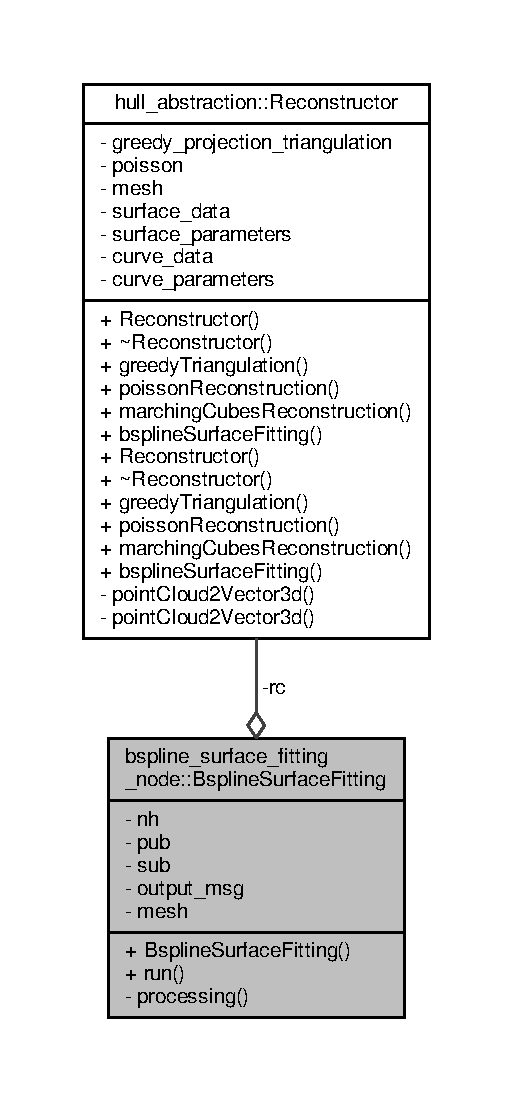
\includegraphics[width=237pt]{classbspline__surface__fitting__node_1_1_bspline_surface_fitting__coll__graph}
\end{center}
\end{figure}
\subsection*{Public Member Functions}
\begin{DoxyCompactItemize}
\item 
\hyperlink{classbspline__surface__fitting__node_1_1_bspline_surface_fitting_a0c6104db4570cd4a865e85d03fae26c3}{Bspline\+Surface\+Fitting} ()
\begin{DoxyCompactList}\small\item\em Construct a new \hyperlink{classbspline__surface__fitting__node_1_1_bspline_surface_fitting}{Bspline\+Surface\+Fitting} object. \end{DoxyCompactList}\item 
void \hyperlink{classbspline__surface__fitting__node_1_1_bspline_surface_fitting_a3ca4a5eb83d40636830e337cac288d03}{run} ()
\begin{DoxyCompactList}\small\item\em Encapsulate a method to run the bspline\+\_\+surface\+\_\+fitting node. \end{DoxyCompactList}\end{DoxyCompactItemize}
\subsection*{Private Member Functions}
\begin{DoxyCompactItemize}
\item 
void \hyperlink{classbspline__surface__fitting__node_1_1_bspline_surface_fitting_a588e2e4f382fc5198b4c17613cf7f03a}{processing} (const sensor\+\_\+msgs\+::\+Point\+Cloud2\+Const\+Ptr input\+\_\+msg)
\begin{DoxyCompactList}\small\item\em Process the input R\+OS message. \end{DoxyCompactList}\end{DoxyCompactItemize}
\subsection*{Private Attributes}
\begin{DoxyCompactItemize}
\item 
ros\+::\+Node\+Handle \hyperlink{classbspline__surface__fitting__node_1_1_bspline_surface_fitting_ab3fb2f277d26f9a58e9575257d035251}{nh}
\item 
ros\+::\+Publisher \hyperlink{classbspline__surface__fitting__node_1_1_bspline_surface_fitting_ac1a664418699fc1f06e5da7637530520}{pub}
\item 
ros\+::\+Subscriber \hyperlink{classbspline__surface__fitting__node_1_1_bspline_surface_fitting_a1ca9460f2069655ce0b55683a6622688}{sub}
\item 
pcl\+\_\+msgs\+::\+Polygon\+Mesh \hyperlink{classbspline__surface__fitting__node_1_1_bspline_surface_fitting_a38d7b7bf42448ad65e7501c19ce859a2}{output\+\_\+msg}
\item 
\hyperlink{classhull__abstraction_1_1_reconstructor}{hull\+\_\+abstraction\+::\+Reconstructor} \hyperlink{classbspline__surface__fitting__node_1_1_bspline_surface_fitting_a37fc14202f71f41647bc78ed21a1f691}{rc}
\item 
pcl\+::\+Polygon\+Mesh \hyperlink{classbspline__surface__fitting__node_1_1_bspline_surface_fitting_a3f3f3a25956432185b5927e0b920a53e}{mesh}
\end{DoxyCompactItemize}


\subsection{Detailed Description}
Class utilizing B-\/spline surface fitting method. 

This framework is developed to generate and publish a mesh for a point cloud through b-\/spline surface fitting. 

\subsection{Constructor \& Destructor Documentation}
\index{bspline\+\_\+surface\+\_\+fitting\+\_\+node\+::\+Bspline\+Surface\+Fitting@{bspline\+\_\+surface\+\_\+fitting\+\_\+node\+::\+Bspline\+Surface\+Fitting}!Bspline\+Surface\+Fitting@{Bspline\+Surface\+Fitting}}
\index{Bspline\+Surface\+Fitting@{Bspline\+Surface\+Fitting}!bspline\+\_\+surface\+\_\+fitting\+\_\+node\+::\+Bspline\+Surface\+Fitting@{bspline\+\_\+surface\+\_\+fitting\+\_\+node\+::\+Bspline\+Surface\+Fitting}}
\subsubsection[{\texorpdfstring{Bspline\+Surface\+Fitting()}{BsplineSurfaceFitting()}}]{\setlength{\rightskip}{0pt plus 5cm}bspline\+\_\+surface\+\_\+fitting\+\_\+node\+::\+Bspline\+Surface\+Fitting\+::\+Bspline\+Surface\+Fitting (
\begin{DoxyParamCaption}
{}
\end{DoxyParamCaption}
)\hspace{0.3cm}{\ttfamily [inline]}}\hypertarget{classbspline__surface__fitting__node_1_1_bspline_surface_fitting_a0c6104db4570cd4a865e85d03fae26c3}{}\label{classbspline__surface__fitting__node_1_1_bspline_surface_fitting_a0c6104db4570cd4a865e85d03fae26c3}


Construct a new \hyperlink{classbspline__surface__fitting__node_1_1_bspline_surface_fitting}{Bspline\+Surface\+Fitting} object. 



\subsection{Member Function Documentation}
\index{bspline\+\_\+surface\+\_\+fitting\+\_\+node\+::\+Bspline\+Surface\+Fitting@{bspline\+\_\+surface\+\_\+fitting\+\_\+node\+::\+Bspline\+Surface\+Fitting}!processing@{processing}}
\index{processing@{processing}!bspline\+\_\+surface\+\_\+fitting\+\_\+node\+::\+Bspline\+Surface\+Fitting@{bspline\+\_\+surface\+\_\+fitting\+\_\+node\+::\+Bspline\+Surface\+Fitting}}
\subsubsection[{\texorpdfstring{processing(const sensor\+\_\+msgs\+::\+Point\+Cloud2\+Const\+Ptr input\+\_\+msg)}{processing(const sensor_msgs::PointCloud2ConstPtr input_msg)}}]{\setlength{\rightskip}{0pt plus 5cm}void bspline\+\_\+surface\+\_\+fitting\+\_\+node\+::\+Bspline\+Surface\+Fitting\+::processing (
\begin{DoxyParamCaption}
\item[{const sensor\+\_\+msgs\+::\+Point\+Cloud2\+Const\+Ptr}]{input\+\_\+msg}
\end{DoxyParamCaption}
)\hspace{0.3cm}{\ttfamily [private]}}\hypertarget{classbspline__surface__fitting__node_1_1_bspline_surface_fitting_a588e2e4f382fc5198b4c17613cf7f03a}{}\label{classbspline__surface__fitting__node_1_1_bspline_surface_fitting_a588e2e4f382fc5198b4c17613cf7f03a}


Process the input R\+OS message. 


\begin{DoxyParams}{Parameters}
{\em input\+\_\+msg} & Input R\+OS message \\
\hline
\end{DoxyParams}
\index{bspline\+\_\+surface\+\_\+fitting\+\_\+node\+::\+Bspline\+Surface\+Fitting@{bspline\+\_\+surface\+\_\+fitting\+\_\+node\+::\+Bspline\+Surface\+Fitting}!run@{run}}
\index{run@{run}!bspline\+\_\+surface\+\_\+fitting\+\_\+node\+::\+Bspline\+Surface\+Fitting@{bspline\+\_\+surface\+\_\+fitting\+\_\+node\+::\+Bspline\+Surface\+Fitting}}
\subsubsection[{\texorpdfstring{run()}{run()}}]{\setlength{\rightskip}{0pt plus 5cm}void bspline\+\_\+surface\+\_\+fitting\+\_\+node\+::\+Bspline\+Surface\+Fitting\+::run (
\begin{DoxyParamCaption}
{}
\end{DoxyParamCaption}
)}\hypertarget{classbspline__surface__fitting__node_1_1_bspline_surface_fitting_a3ca4a5eb83d40636830e337cac288d03}{}\label{classbspline__surface__fitting__node_1_1_bspline_surface_fitting_a3ca4a5eb83d40636830e337cac288d03}


Encapsulate a method to run the bspline\+\_\+surface\+\_\+fitting node. 



\subsection{Member Data Documentation}
\index{bspline\+\_\+surface\+\_\+fitting\+\_\+node\+::\+Bspline\+Surface\+Fitting@{bspline\+\_\+surface\+\_\+fitting\+\_\+node\+::\+Bspline\+Surface\+Fitting}!mesh@{mesh}}
\index{mesh@{mesh}!bspline\+\_\+surface\+\_\+fitting\+\_\+node\+::\+Bspline\+Surface\+Fitting@{bspline\+\_\+surface\+\_\+fitting\+\_\+node\+::\+Bspline\+Surface\+Fitting}}
\subsubsection[{\texorpdfstring{mesh}{mesh}}]{\setlength{\rightskip}{0pt plus 5cm}pcl\+::\+Polygon\+Mesh bspline\+\_\+surface\+\_\+fitting\+\_\+node\+::\+Bspline\+Surface\+Fitting\+::mesh\hspace{0.3cm}{\ttfamily [private]}}\hypertarget{classbspline__surface__fitting__node_1_1_bspline_surface_fitting_a3f3f3a25956432185b5927e0b920a53e}{}\label{classbspline__surface__fitting__node_1_1_bspline_surface_fitting_a3f3f3a25956432185b5927e0b920a53e}
Resulted polygon mesh \index{bspline\+\_\+surface\+\_\+fitting\+\_\+node\+::\+Bspline\+Surface\+Fitting@{bspline\+\_\+surface\+\_\+fitting\+\_\+node\+::\+Bspline\+Surface\+Fitting}!nh@{nh}}
\index{nh@{nh}!bspline\+\_\+surface\+\_\+fitting\+\_\+node\+::\+Bspline\+Surface\+Fitting@{bspline\+\_\+surface\+\_\+fitting\+\_\+node\+::\+Bspline\+Surface\+Fitting}}
\subsubsection[{\texorpdfstring{nh}{nh}}]{\setlength{\rightskip}{0pt plus 5cm}ros\+::\+Node\+Handle bspline\+\_\+surface\+\_\+fitting\+\_\+node\+::\+Bspline\+Surface\+Fitting\+::nh\hspace{0.3cm}{\ttfamily [private]}}\hypertarget{classbspline__surface__fitting__node_1_1_bspline_surface_fitting_ab3fb2f277d26f9a58e9575257d035251}{}\label{classbspline__surface__fitting__node_1_1_bspline_surface_fitting_ab3fb2f277d26f9a58e9575257d035251}
Node Handle reference from embedding node \index{bspline\+\_\+surface\+\_\+fitting\+\_\+node\+::\+Bspline\+Surface\+Fitting@{bspline\+\_\+surface\+\_\+fitting\+\_\+node\+::\+Bspline\+Surface\+Fitting}!output\+\_\+msg@{output\+\_\+msg}}
\index{output\+\_\+msg@{output\+\_\+msg}!bspline\+\_\+surface\+\_\+fitting\+\_\+node\+::\+Bspline\+Surface\+Fitting@{bspline\+\_\+surface\+\_\+fitting\+\_\+node\+::\+Bspline\+Surface\+Fitting}}
\subsubsection[{\texorpdfstring{output\+\_\+msg}{output_msg}}]{\setlength{\rightskip}{0pt plus 5cm}pcl\+\_\+msgs\+::\+Polygon\+Mesh bspline\+\_\+surface\+\_\+fitting\+\_\+node\+::\+Bspline\+Surface\+Fitting\+::output\+\_\+msg\hspace{0.3cm}{\ttfamily [private]}}\hypertarget{classbspline__surface__fitting__node_1_1_bspline_surface_fitting_a38d7b7bf42448ad65e7501c19ce859a2}{}\label{classbspline__surface__fitting__node_1_1_bspline_surface_fitting_a38d7b7bf42448ad65e7501c19ce859a2}
Polygon mesh message used to publish the mesh \index{bspline\+\_\+surface\+\_\+fitting\+\_\+node\+::\+Bspline\+Surface\+Fitting@{bspline\+\_\+surface\+\_\+fitting\+\_\+node\+::\+Bspline\+Surface\+Fitting}!pub@{pub}}
\index{pub@{pub}!bspline\+\_\+surface\+\_\+fitting\+\_\+node\+::\+Bspline\+Surface\+Fitting@{bspline\+\_\+surface\+\_\+fitting\+\_\+node\+::\+Bspline\+Surface\+Fitting}}
\subsubsection[{\texorpdfstring{pub}{pub}}]{\setlength{\rightskip}{0pt plus 5cm}ros\+::\+Publisher bspline\+\_\+surface\+\_\+fitting\+\_\+node\+::\+Bspline\+Surface\+Fitting\+::pub\hspace{0.3cm}{\ttfamily [private]}}\hypertarget{classbspline__surface__fitting__node_1_1_bspline_surface_fitting_ac1a664418699fc1f06e5da7637530520}{}\label{classbspline__surface__fitting__node_1_1_bspline_surface_fitting_ac1a664418699fc1f06e5da7637530520}
Polygon mesh publisher \index{bspline\+\_\+surface\+\_\+fitting\+\_\+node\+::\+Bspline\+Surface\+Fitting@{bspline\+\_\+surface\+\_\+fitting\+\_\+node\+::\+Bspline\+Surface\+Fitting}!rc@{rc}}
\index{rc@{rc}!bspline\+\_\+surface\+\_\+fitting\+\_\+node\+::\+Bspline\+Surface\+Fitting@{bspline\+\_\+surface\+\_\+fitting\+\_\+node\+::\+Bspline\+Surface\+Fitting}}
\subsubsection[{\texorpdfstring{rc}{rc}}]{\setlength{\rightskip}{0pt plus 5cm}{\bf hull\+\_\+abstraction\+::\+Reconstructor} bspline\+\_\+surface\+\_\+fitting\+\_\+node\+::\+Bspline\+Surface\+Fitting\+::rc\hspace{0.3cm}{\ttfamily [private]}}\hypertarget{classbspline__surface__fitting__node_1_1_bspline_surface_fitting_a37fc14202f71f41647bc78ed21a1f691}{}\label{classbspline__surface__fitting__node_1_1_bspline_surface_fitting_a37fc14202f71f41647bc78ed21a1f691}
Object for Reconstructor class \index{bspline\+\_\+surface\+\_\+fitting\+\_\+node\+::\+Bspline\+Surface\+Fitting@{bspline\+\_\+surface\+\_\+fitting\+\_\+node\+::\+Bspline\+Surface\+Fitting}!sub@{sub}}
\index{sub@{sub}!bspline\+\_\+surface\+\_\+fitting\+\_\+node\+::\+Bspline\+Surface\+Fitting@{bspline\+\_\+surface\+\_\+fitting\+\_\+node\+::\+Bspline\+Surface\+Fitting}}
\subsubsection[{\texorpdfstring{sub}{sub}}]{\setlength{\rightskip}{0pt plus 5cm}ros\+::\+Subscriber bspline\+\_\+surface\+\_\+fitting\+\_\+node\+::\+Bspline\+Surface\+Fitting\+::sub\hspace{0.3cm}{\ttfamily [private]}}\hypertarget{classbspline__surface__fitting__node_1_1_bspline_surface_fitting_a1ca9460f2069655ce0b55683a6622688}{}\label{classbspline__surface__fitting__node_1_1_bspline_surface_fitting_a1ca9460f2069655ce0b55683a6622688}
Raw point cloud subscriber 

The documentation for this class was generated from the following files\+:\begin{DoxyCompactItemize}
\item 
/home/jc/\+T\+H\+E\+S\+I\+S/hull\+\_\+abstraction/ros/src/hull\+\_\+abstraction/src/bspline\+\_\+surface\+\_\+fitting\+\_\+node/\hyperlink{bspline__surface__fitting_8h}{bspline\+\_\+surface\+\_\+fitting.\+h}\item 
/home/jc/\+T\+H\+E\+S\+I\+S/hull\+\_\+abstraction/ros/src/hull\+\_\+abstraction/src/bspline\+\_\+surface\+\_\+fitting\+\_\+node/\hyperlink{bspline__surface__fitting_8cpp}{bspline\+\_\+surface\+\_\+fitting.\+cpp}\end{DoxyCompactItemize}

\hypertarget{classdisplay__mesh_1_1_display_mesh}{}\section{display\+\_\+mesh\+:\+:Display\+Mesh Class Reference}
\label{classdisplay__mesh_1_1_display_mesh}\index{display\+\_\+mesh\+::\+Display\+Mesh@{display\+\_\+mesh\+::\+Display\+Mesh}}


Class for displaying mesh in R\+V\+IZ.  




{\ttfamily \#include $<$display\+\_\+mesh.\+h$>$}



Collaboration diagram for display\+\_\+mesh\+:\+:Display\+Mesh\+:\nopagebreak
\begin{figure}[H]
\begin{center}
\leavevmode
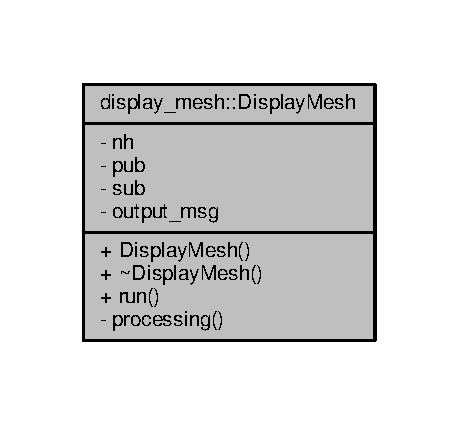
\includegraphics[width=220pt]{classdisplay__mesh_1_1_display_mesh__coll__graph}
\end{center}
\end{figure}
\subsection*{Public Member Functions}
\begin{DoxyCompactItemize}
\item 
\hyperlink{classdisplay__mesh_1_1_display_mesh_a75e143fd00c1a1b777eea976f8580030}{Display\+Mesh} ()
\begin{DoxyCompactList}\small\item\em Construct a new Display Mesh object. \end{DoxyCompactList}\item 
\hyperlink{classdisplay__mesh_1_1_display_mesh_a39727abcea404714b69aa465dd6df4bb}{$\sim$\+Display\+Mesh} ()
\begin{DoxyCompactList}\small\item\em Destroy the Display Mesh object. \end{DoxyCompactList}\item 
void \hyperlink{classdisplay__mesh_1_1_display_mesh_ac41b88adcb0deeaa2d4febee382c4f14}{run} ()
\begin{DoxyCompactList}\small\item\em Encapsulate a method to run the \hyperlink{namespacedisplay__mesh}{display\+\_\+mesh} node. \end{DoxyCompactList}\end{DoxyCompactItemize}
\subsection*{Private Member Functions}
\begin{DoxyCompactItemize}
\item 
void \hyperlink{classdisplay__mesh_1_1_display_mesh_ab6c8cea34f5e67c9ac0b578da6e9f517}{processing} (const pcl\+\_\+msgs\+::\+Polygon\+Mesh input\+\_\+msg)
\begin{DoxyCompactList}\small\item\em Process the point cloud message to create mesh message. \end{DoxyCompactList}\end{DoxyCompactItemize}
\subsection*{Private Attributes}
\begin{DoxyCompactItemize}
\item 
ros\+::\+Node\+Handle \hyperlink{classdisplay__mesh_1_1_display_mesh_a8d788cd12e7e9b670da079478f3231c3}{nh}
\item 
ros\+::\+Publisher \hyperlink{classdisplay__mesh_1_1_display_mesh_ad2ede578fe0dae783e9e06942441e2be}{pub}
\item 
ros\+::\+Subscriber \hyperlink{classdisplay__mesh_1_1_display_mesh_a0cef4c6f1b95ba3ad39a470e277bbe7e}{sub}
\item 
visualization\+\_\+msgs\+::\+Marker \hyperlink{classdisplay__mesh_1_1_display_mesh_a950554fa9242f3d358e1085955e37a5b}{output\+\_\+msg}
\end{DoxyCompactItemize}


\subsection{Detailed Description}
Class for displaying mesh in R\+V\+IZ. 

\subsection{Constructor \& Destructor Documentation}
\index{display\+\_\+mesh\+::\+Display\+Mesh@{display\+\_\+mesh\+::\+Display\+Mesh}!Display\+Mesh@{Display\+Mesh}}
\index{Display\+Mesh@{Display\+Mesh}!display\+\_\+mesh\+::\+Display\+Mesh@{display\+\_\+mesh\+::\+Display\+Mesh}}
\subsubsection[{\texorpdfstring{Display\+Mesh()}{DisplayMesh()}}]{\setlength{\rightskip}{0pt plus 5cm}display\+\_\+mesh\+::\+Display\+Mesh\+::\+Display\+Mesh (
\begin{DoxyParamCaption}
{}
\end{DoxyParamCaption}
)\hspace{0.3cm}{\ttfamily [inline]}}\hypertarget{classdisplay__mesh_1_1_display_mesh_a75e143fd00c1a1b777eea976f8580030}{}\label{classdisplay__mesh_1_1_display_mesh_a75e143fd00c1a1b777eea976f8580030}


Construct a new Display Mesh object. 

\index{display\+\_\+mesh\+::\+Display\+Mesh@{display\+\_\+mesh\+::\+Display\+Mesh}!````~Display\+Mesh@{$\sim$\+Display\+Mesh}}
\index{````~Display\+Mesh@{$\sim$\+Display\+Mesh}!display\+\_\+mesh\+::\+Display\+Mesh@{display\+\_\+mesh\+::\+Display\+Mesh}}
\subsubsection[{\texorpdfstring{$\sim$\+Display\+Mesh()}{~DisplayMesh()}}]{\setlength{\rightskip}{0pt plus 5cm}display\+\_\+mesh\+::\+Display\+Mesh\+::$\sim$\+Display\+Mesh (
\begin{DoxyParamCaption}
{}
\end{DoxyParamCaption}
)\hspace{0.3cm}{\ttfamily [inline]}}\hypertarget{classdisplay__mesh_1_1_display_mesh_a39727abcea404714b69aa465dd6df4bb}{}\label{classdisplay__mesh_1_1_display_mesh_a39727abcea404714b69aa465dd6df4bb}


Destroy the Display Mesh object. 



\subsection{Member Function Documentation}
\index{display\+\_\+mesh\+::\+Display\+Mesh@{display\+\_\+mesh\+::\+Display\+Mesh}!processing@{processing}}
\index{processing@{processing}!display\+\_\+mesh\+::\+Display\+Mesh@{display\+\_\+mesh\+::\+Display\+Mesh}}
\subsubsection[{\texorpdfstring{processing(const pcl\+\_\+msgs\+::\+Polygon\+Mesh input\+\_\+msg)}{processing(const pcl_msgs::PolygonMesh input_msg)}}]{\setlength{\rightskip}{0pt plus 5cm}void display\+\_\+mesh\+::\+Display\+Mesh\+::processing (
\begin{DoxyParamCaption}
\item[{const pcl\+\_\+msgs\+::\+Polygon\+Mesh}]{input\+\_\+msg}
\end{DoxyParamCaption}
)\hspace{0.3cm}{\ttfamily [private]}}\hypertarget{classdisplay__mesh_1_1_display_mesh_ab6c8cea34f5e67c9ac0b578da6e9f517}{}\label{classdisplay__mesh_1_1_display_mesh_ab6c8cea34f5e67c9ac0b578da6e9f517}


Process the point cloud message to create mesh message. 


\begin{DoxyParams}{Parameters}
{\em input\+\_\+msg} & Input point cloud message \\
\hline
\end{DoxyParams}
\index{display\+\_\+mesh\+::\+Display\+Mesh@{display\+\_\+mesh\+::\+Display\+Mesh}!run@{run}}
\index{run@{run}!display\+\_\+mesh\+::\+Display\+Mesh@{display\+\_\+mesh\+::\+Display\+Mesh}}
\subsubsection[{\texorpdfstring{run()}{run()}}]{\setlength{\rightskip}{0pt plus 5cm}void display\+\_\+mesh\+::\+Display\+Mesh\+::run (
\begin{DoxyParamCaption}
{}
\end{DoxyParamCaption}
)}\hypertarget{classdisplay__mesh_1_1_display_mesh_ac41b88adcb0deeaa2d4febee382c4f14}{}\label{classdisplay__mesh_1_1_display_mesh_ac41b88adcb0deeaa2d4febee382c4f14}


Encapsulate a method to run the \hyperlink{namespacedisplay__mesh}{display\+\_\+mesh} node. 


\begin{DoxyParams}{Parameters}
{\em topic} & Name of topic for input point cloud message \\
\hline
\end{DoxyParams}


\subsection{Member Data Documentation}
\index{display\+\_\+mesh\+::\+Display\+Mesh@{display\+\_\+mesh\+::\+Display\+Mesh}!nh@{nh}}
\index{nh@{nh}!display\+\_\+mesh\+::\+Display\+Mesh@{display\+\_\+mesh\+::\+Display\+Mesh}}
\subsubsection[{\texorpdfstring{nh}{nh}}]{\setlength{\rightskip}{0pt plus 5cm}ros\+::\+Node\+Handle display\+\_\+mesh\+::\+Display\+Mesh\+::nh\hspace{0.3cm}{\ttfamily [private]}}\hypertarget{classdisplay__mesh_1_1_display_mesh_a8d788cd12e7e9b670da079478f3231c3}{}\label{classdisplay__mesh_1_1_display_mesh_a8d788cd12e7e9b670da079478f3231c3}
Node Handle reference from embedding node \index{display\+\_\+mesh\+::\+Display\+Mesh@{display\+\_\+mesh\+::\+Display\+Mesh}!output\+\_\+msg@{output\+\_\+msg}}
\index{output\+\_\+msg@{output\+\_\+msg}!display\+\_\+mesh\+::\+Display\+Mesh@{display\+\_\+mesh\+::\+Display\+Mesh}}
\subsubsection[{\texorpdfstring{output\+\_\+msg}{output_msg}}]{\setlength{\rightskip}{0pt plus 5cm}visualization\+\_\+msgs\+::\+Marker display\+\_\+mesh\+::\+Display\+Mesh\+::output\+\_\+msg\hspace{0.3cm}{\ttfamily [private]}}\hypertarget{classdisplay__mesh_1_1_display_mesh_a950554fa9242f3d358e1085955e37a5b}{}\label{classdisplay__mesh_1_1_display_mesh_a950554fa9242f3d358e1085955e37a5b}
Marker message used to publish the mesh \index{display\+\_\+mesh\+::\+Display\+Mesh@{display\+\_\+mesh\+::\+Display\+Mesh}!pub@{pub}}
\index{pub@{pub}!display\+\_\+mesh\+::\+Display\+Mesh@{display\+\_\+mesh\+::\+Display\+Mesh}}
\subsubsection[{\texorpdfstring{pub}{pub}}]{\setlength{\rightskip}{0pt plus 5cm}ros\+::\+Publisher display\+\_\+mesh\+::\+Display\+Mesh\+::pub\hspace{0.3cm}{\ttfamily [private]}}\hypertarget{classdisplay__mesh_1_1_display_mesh_ad2ede578fe0dae783e9e06942441e2be}{}\label{classdisplay__mesh_1_1_display_mesh_ad2ede578fe0dae783e9e06942441e2be}
Point cloud publisher \index{display\+\_\+mesh\+::\+Display\+Mesh@{display\+\_\+mesh\+::\+Display\+Mesh}!sub@{sub}}
\index{sub@{sub}!display\+\_\+mesh\+::\+Display\+Mesh@{display\+\_\+mesh\+::\+Display\+Mesh}}
\subsubsection[{\texorpdfstring{sub}{sub}}]{\setlength{\rightskip}{0pt plus 5cm}ros\+::\+Subscriber display\+\_\+mesh\+::\+Display\+Mesh\+::sub\hspace{0.3cm}{\ttfamily [private]}}\hypertarget{classdisplay__mesh_1_1_display_mesh_a0cef4c6f1b95ba3ad39a470e277bbe7e}{}\label{classdisplay__mesh_1_1_display_mesh_a0cef4c6f1b95ba3ad39a470e277bbe7e}
Raw point cloud subscriber 

The documentation for this class was generated from the following files\+:\begin{DoxyCompactItemize}
\item 
/home/jc/hull\+\_\+abstraction/ros/src/hull\+\_\+abstraction/src/display\+\_\+mesh\+\_\+node/\hyperlink{display__mesh_8h}{display\+\_\+mesh.\+h}\item 
/home/jc/hull\+\_\+abstraction/ros/src/hull\+\_\+abstraction/src/display\+\_\+mesh\+\_\+node/\hyperlink{display__mesh_8cpp}{display\+\_\+mesh.\+cpp}\end{DoxyCompactItemize}

\hypertarget{classgreedy__triangulation_1_1_greedy_triangulation}{}\section{greedy\+\_\+triangulation\+:\+:Greedy\+Triangulation Class Reference}
\label{classgreedy__triangulation_1_1_greedy_triangulation}\index{greedy\+\_\+triangulation\+::\+Greedy\+Triangulation@{greedy\+\_\+triangulation\+::\+Greedy\+Triangulation}}


Class utilizing greedy triangulation method.  




{\ttfamily \#include $<$greedy\+\_\+triangulation.\+h$>$}



Collaboration diagram for greedy\+\_\+triangulation\+:\+:Greedy\+Triangulation\+:\nopagebreak
\begin{figure}[H]
\begin{center}
\leavevmode
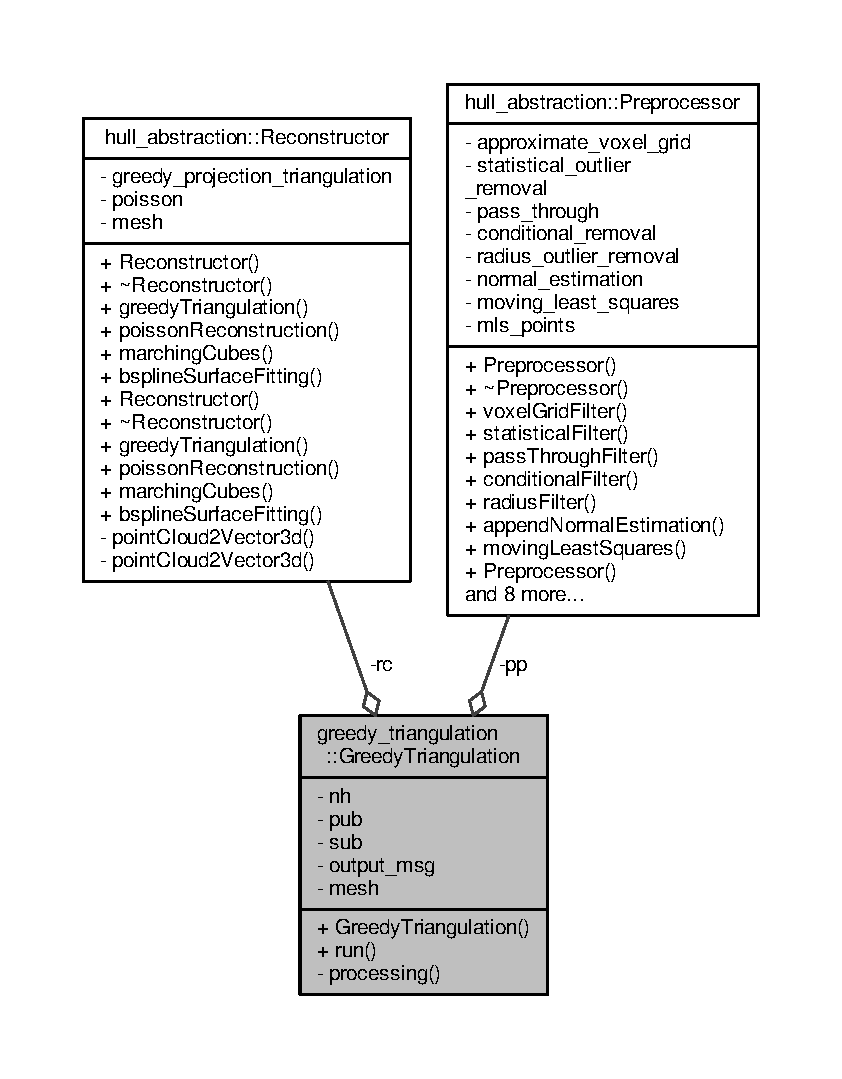
\includegraphics[width=350pt]{classgreedy__triangulation_1_1_greedy_triangulation__coll__graph}
\end{center}
\end{figure}
\subsection*{Public Member Functions}
\begin{DoxyCompactItemize}
\item 
\hyperlink{classgreedy__triangulation_1_1_greedy_triangulation_aa72aa5549f91496308e74182524c20ba}{Greedy\+Triangulation} ()
\begin{DoxyCompactList}\small\item\em Construct a new \hyperlink{classgreedy__triangulation_1_1_greedy_triangulation}{Greedy\+Triangulation} object. \end{DoxyCompactList}\item 
void \hyperlink{classgreedy__triangulation_1_1_greedy_triangulation_ac8a14592c912234b10fec99bc11b6fe9}{run} ()
\begin{DoxyCompactList}\small\item\em Encapsulate a method to run the \hyperlink{namespacegreedy__triangulation}{greedy\+\_\+triangulation} node. \end{DoxyCompactList}\end{DoxyCompactItemize}
\subsection*{Private Member Functions}
\begin{DoxyCompactItemize}
\item 
void \hyperlink{classgreedy__triangulation_1_1_greedy_triangulation_a202974e4b7bfda702b2abde1894e2526}{processing} (const sensor\+\_\+msgs\+::\+Point\+Cloud2\+Const\+Ptr input\+\_\+msg)
\begin{DoxyCompactList}\small\item\em Process the point cloud message to create mesh message. \end{DoxyCompactList}\end{DoxyCompactItemize}
\subsection*{Private Attributes}
\begin{DoxyCompactItemize}
\item 
ros\+::\+Node\+Handle \hyperlink{classgreedy__triangulation_1_1_greedy_triangulation_aaf891e65ede2c18d5f20fbfeadcd2083}{nh}
\item 
ros\+::\+Publisher \hyperlink{classgreedy__triangulation_1_1_greedy_triangulation_a6ca8884fc1b5b2fcd5fc4c9c7c290451}{pub}
\item 
ros\+::\+Subscriber \hyperlink{classgreedy__triangulation_1_1_greedy_triangulation_afb3a088f4a5b177363eae83a1187ed58}{sub}
\item 
pcl\+\_\+msgs\+::\+Polygon\+Mesh \hyperlink{classgreedy__triangulation_1_1_greedy_triangulation_acd6529152058723f54dd5e9f1d0b040d}{output\+\_\+msg}
\item 
\hyperlink{classhull__abstraction_1_1_reconstructor}{hull\+\_\+abstraction\+::\+Reconstructor} \hyperlink{classgreedy__triangulation_1_1_greedy_triangulation_a69a1c245b9985fe03482884cf54b851d}{rc}
\item 
\hyperlink{classhull__abstraction_1_1_preprocessor}{hull\+\_\+abstraction\+::\+Preprocessor} \hyperlink{classgreedy__triangulation_1_1_greedy_triangulation_a9f5ea346f74bd3352a341319a6bb2e53}{pp}
\item 
pcl\+::\+Polygon\+Mesh \hyperlink{classgreedy__triangulation_1_1_greedy_triangulation_a0262f92de8d002b650dbc1b05ebe67dc}{mesh}
\end{DoxyCompactItemize}


\subsection{Detailed Description}
Class utilizing greedy triangulation method. 

This framework is developed to generate a mesh for a point cloud through greedy triangulation. 

\subsection{Constructor \& Destructor Documentation}
\index{greedy\+\_\+triangulation\+::\+Greedy\+Triangulation@{greedy\+\_\+triangulation\+::\+Greedy\+Triangulation}!Greedy\+Triangulation@{Greedy\+Triangulation}}
\index{Greedy\+Triangulation@{Greedy\+Triangulation}!greedy\+\_\+triangulation\+::\+Greedy\+Triangulation@{greedy\+\_\+triangulation\+::\+Greedy\+Triangulation}}
\subsubsection[{\texorpdfstring{Greedy\+Triangulation()}{GreedyTriangulation()}}]{\setlength{\rightskip}{0pt plus 5cm}greedy\+\_\+triangulation\+::\+Greedy\+Triangulation\+::\+Greedy\+Triangulation (
\begin{DoxyParamCaption}
{}
\end{DoxyParamCaption}
)\hspace{0.3cm}{\ttfamily [inline]}}\hypertarget{classgreedy__triangulation_1_1_greedy_triangulation_aa72aa5549f91496308e74182524c20ba}{}\label{classgreedy__triangulation_1_1_greedy_triangulation_aa72aa5549f91496308e74182524c20ba}


Construct a new \hyperlink{classgreedy__triangulation_1_1_greedy_triangulation}{Greedy\+Triangulation} object. 



\subsection{Member Function Documentation}
\index{greedy\+\_\+triangulation\+::\+Greedy\+Triangulation@{greedy\+\_\+triangulation\+::\+Greedy\+Triangulation}!processing@{processing}}
\index{processing@{processing}!greedy\+\_\+triangulation\+::\+Greedy\+Triangulation@{greedy\+\_\+triangulation\+::\+Greedy\+Triangulation}}
\subsubsection[{\texorpdfstring{processing(const sensor\+\_\+msgs\+::\+Point\+Cloud2\+Const\+Ptr input\+\_\+msg)}{processing(const sensor_msgs::PointCloud2ConstPtr input_msg)}}]{\setlength{\rightskip}{0pt plus 5cm}void greedy\+\_\+triangulation\+::\+Greedy\+Triangulation\+::processing (
\begin{DoxyParamCaption}
\item[{const sensor\+\_\+msgs\+::\+Point\+Cloud2\+Const\+Ptr}]{input\+\_\+msg}
\end{DoxyParamCaption}
)\hspace{0.3cm}{\ttfamily [private]}}\hypertarget{classgreedy__triangulation_1_1_greedy_triangulation_a202974e4b7bfda702b2abde1894e2526}{}\label{classgreedy__triangulation_1_1_greedy_triangulation_a202974e4b7bfda702b2abde1894e2526}


Process the point cloud message to create mesh message. 


\begin{DoxyParams}{Parameters}
{\em input\+\_\+msg} & Input point cloud message \\
\hline
\end{DoxyParams}
\index{greedy\+\_\+triangulation\+::\+Greedy\+Triangulation@{greedy\+\_\+triangulation\+::\+Greedy\+Triangulation}!run@{run}}
\index{run@{run}!greedy\+\_\+triangulation\+::\+Greedy\+Triangulation@{greedy\+\_\+triangulation\+::\+Greedy\+Triangulation}}
\subsubsection[{\texorpdfstring{run()}{run()}}]{\setlength{\rightskip}{0pt plus 5cm}void greedy\+\_\+triangulation\+::\+Greedy\+Triangulation\+::run (
\begin{DoxyParamCaption}
{}
\end{DoxyParamCaption}
)}\hypertarget{classgreedy__triangulation_1_1_greedy_triangulation_ac8a14592c912234b10fec99bc11b6fe9}{}\label{classgreedy__triangulation_1_1_greedy_triangulation_ac8a14592c912234b10fec99bc11b6fe9}


Encapsulate a method to run the \hyperlink{namespacegreedy__triangulation}{greedy\+\_\+triangulation} node. 



\subsection{Member Data Documentation}
\index{greedy\+\_\+triangulation\+::\+Greedy\+Triangulation@{greedy\+\_\+triangulation\+::\+Greedy\+Triangulation}!mesh@{mesh}}
\index{mesh@{mesh}!greedy\+\_\+triangulation\+::\+Greedy\+Triangulation@{greedy\+\_\+triangulation\+::\+Greedy\+Triangulation}}
\subsubsection[{\texorpdfstring{mesh}{mesh}}]{\setlength{\rightskip}{0pt plus 5cm}pcl\+::\+Polygon\+Mesh greedy\+\_\+triangulation\+::\+Greedy\+Triangulation\+::mesh\hspace{0.3cm}{\ttfamily [private]}}\hypertarget{classgreedy__triangulation_1_1_greedy_triangulation_a0262f92de8d002b650dbc1b05ebe67dc}{}\label{classgreedy__triangulation_1_1_greedy_triangulation_a0262f92de8d002b650dbc1b05ebe67dc}
Resulted polygon mesh \index{greedy\+\_\+triangulation\+::\+Greedy\+Triangulation@{greedy\+\_\+triangulation\+::\+Greedy\+Triangulation}!nh@{nh}}
\index{nh@{nh}!greedy\+\_\+triangulation\+::\+Greedy\+Triangulation@{greedy\+\_\+triangulation\+::\+Greedy\+Triangulation}}
\subsubsection[{\texorpdfstring{nh}{nh}}]{\setlength{\rightskip}{0pt plus 5cm}ros\+::\+Node\+Handle greedy\+\_\+triangulation\+::\+Greedy\+Triangulation\+::nh\hspace{0.3cm}{\ttfamily [private]}}\hypertarget{classgreedy__triangulation_1_1_greedy_triangulation_aaf891e65ede2c18d5f20fbfeadcd2083}{}\label{classgreedy__triangulation_1_1_greedy_triangulation_aaf891e65ede2c18d5f20fbfeadcd2083}
Node Handle reference from embedding node \index{greedy\+\_\+triangulation\+::\+Greedy\+Triangulation@{greedy\+\_\+triangulation\+::\+Greedy\+Triangulation}!output\+\_\+msg@{output\+\_\+msg}}
\index{output\+\_\+msg@{output\+\_\+msg}!greedy\+\_\+triangulation\+::\+Greedy\+Triangulation@{greedy\+\_\+triangulation\+::\+Greedy\+Triangulation}}
\subsubsection[{\texorpdfstring{output\+\_\+msg}{output_msg}}]{\setlength{\rightskip}{0pt plus 5cm}pcl\+\_\+msgs\+::\+Polygon\+Mesh greedy\+\_\+triangulation\+::\+Greedy\+Triangulation\+::output\+\_\+msg\hspace{0.3cm}{\ttfamily [private]}}\hypertarget{classgreedy__triangulation_1_1_greedy_triangulation_acd6529152058723f54dd5e9f1d0b040d}{}\label{classgreedy__triangulation_1_1_greedy_triangulation_acd6529152058723f54dd5e9f1d0b040d}
Polygon mesh message used to publish the mesh \index{greedy\+\_\+triangulation\+::\+Greedy\+Triangulation@{greedy\+\_\+triangulation\+::\+Greedy\+Triangulation}!pp@{pp}}
\index{pp@{pp}!greedy\+\_\+triangulation\+::\+Greedy\+Triangulation@{greedy\+\_\+triangulation\+::\+Greedy\+Triangulation}}
\subsubsection[{\texorpdfstring{pp}{pp}}]{\setlength{\rightskip}{0pt plus 5cm}{\bf hull\+\_\+abstraction\+::\+Preprocessor} greedy\+\_\+triangulation\+::\+Greedy\+Triangulation\+::pp\hspace{0.3cm}{\ttfamily [private]}}\hypertarget{classgreedy__triangulation_1_1_greedy_triangulation_a9f5ea346f74bd3352a341319a6bb2e53}{}\label{classgreedy__triangulation_1_1_greedy_triangulation_a9f5ea346f74bd3352a341319a6bb2e53}
Object for Preprocessor class \index{greedy\+\_\+triangulation\+::\+Greedy\+Triangulation@{greedy\+\_\+triangulation\+::\+Greedy\+Triangulation}!pub@{pub}}
\index{pub@{pub}!greedy\+\_\+triangulation\+::\+Greedy\+Triangulation@{greedy\+\_\+triangulation\+::\+Greedy\+Triangulation}}
\subsubsection[{\texorpdfstring{pub}{pub}}]{\setlength{\rightskip}{0pt plus 5cm}ros\+::\+Publisher greedy\+\_\+triangulation\+::\+Greedy\+Triangulation\+::pub\hspace{0.3cm}{\ttfamily [private]}}\hypertarget{classgreedy__triangulation_1_1_greedy_triangulation_a6ca8884fc1b5b2fcd5fc4c9c7c290451}{}\label{classgreedy__triangulation_1_1_greedy_triangulation_a6ca8884fc1b5b2fcd5fc4c9c7c290451}
Polygon mesh publisher \index{greedy\+\_\+triangulation\+::\+Greedy\+Triangulation@{greedy\+\_\+triangulation\+::\+Greedy\+Triangulation}!rc@{rc}}
\index{rc@{rc}!greedy\+\_\+triangulation\+::\+Greedy\+Triangulation@{greedy\+\_\+triangulation\+::\+Greedy\+Triangulation}}
\subsubsection[{\texorpdfstring{rc}{rc}}]{\setlength{\rightskip}{0pt plus 5cm}{\bf hull\+\_\+abstraction\+::\+Reconstructor} greedy\+\_\+triangulation\+::\+Greedy\+Triangulation\+::rc\hspace{0.3cm}{\ttfamily [private]}}\hypertarget{classgreedy__triangulation_1_1_greedy_triangulation_a69a1c245b9985fe03482884cf54b851d}{}\label{classgreedy__triangulation_1_1_greedy_triangulation_a69a1c245b9985fe03482884cf54b851d}
Object for Reconstructor class \index{greedy\+\_\+triangulation\+::\+Greedy\+Triangulation@{greedy\+\_\+triangulation\+::\+Greedy\+Triangulation}!sub@{sub}}
\index{sub@{sub}!greedy\+\_\+triangulation\+::\+Greedy\+Triangulation@{greedy\+\_\+triangulation\+::\+Greedy\+Triangulation}}
\subsubsection[{\texorpdfstring{sub}{sub}}]{\setlength{\rightskip}{0pt plus 5cm}ros\+::\+Subscriber greedy\+\_\+triangulation\+::\+Greedy\+Triangulation\+::sub\hspace{0.3cm}{\ttfamily [private]}}\hypertarget{classgreedy__triangulation_1_1_greedy_triangulation_afb3a088f4a5b177363eae83a1187ed58}{}\label{classgreedy__triangulation_1_1_greedy_triangulation_afb3a088f4a5b177363eae83a1187ed58}
Raw point cloud subscriber 

The documentation for this class was generated from the following files\+:\begin{DoxyCompactItemize}
\item 
/home/jc/\+T\+H\+E\+S\+I\+S/hull\+\_\+abstraction/ros/src/hull\+\_\+abstraction/src/greedy\+\_\+triangulation\+\_\+node/\hyperlink{greedy__triangulation_8h}{greedy\+\_\+triangulation.\+h}\item 
/home/jc/\+T\+H\+E\+S\+I\+S/hull\+\_\+abstraction/ros/src/hull\+\_\+abstraction/src/greedy\+\_\+triangulation\+\_\+node/\hyperlink{greedy__triangulation_8cpp}{greedy\+\_\+triangulation.\+cpp}\end{DoxyCompactItemize}

\hypertarget{classload__pcd_1_1_load_p_c_d}{}\section{load\+\_\+pcd\+:\+:Load\+P\+CD Class Reference}
\label{classload__pcd_1_1_load_p_c_d}\index{load\+\_\+pcd\+::\+Load\+P\+CD@{load\+\_\+pcd\+::\+Load\+P\+CD}}


Class for loading pcd files.  




{\ttfamily \#include $<$load\+\_\+pcd.\+h$>$}



Collaboration diagram for load\+\_\+pcd\+:\+:Load\+P\+CD\+:\nopagebreak
\begin{figure}[H]
\begin{center}
\leavevmode
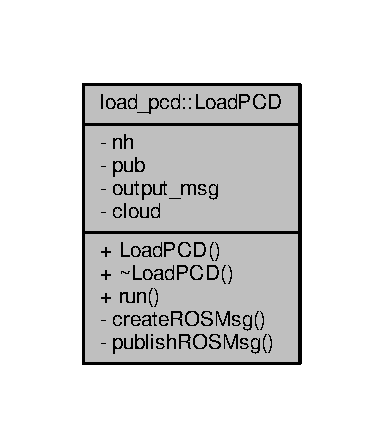
\includegraphics[width=184pt]{classload__pcd_1_1_load_p_c_d__coll__graph}
\end{center}
\end{figure}
\subsection*{Public Member Functions}
\begin{DoxyCompactItemize}
\item 
\hyperlink{classload__pcd_1_1_load_p_c_d_a3fd11130cec167f69b6061009dc84748}{Load\+P\+CD} ()
\begin{DoxyCompactList}\small\item\em Construct a new \hyperlink{classload__pcd_1_1_load_p_c_d}{Load\+P\+CD} object. \end{DoxyCompactList}\item 
\hyperlink{classload__pcd_1_1_load_p_c_d_a48acb121f4dd61dcc3f7da12a300b8ba}{$\sim$\+Load\+P\+CD} ()
\begin{DoxyCompactList}\small\item\em Destroy the \hyperlink{classload__pcd_1_1_load_p_c_d}{Load\+P\+CD} object. \end{DoxyCompactList}\item 
void \hyperlink{classload__pcd_1_1_load_p_c_d_a724e71f567347d242039611c423db5c8}{run} ()
\begin{DoxyCompactList}\small\item\em Encapsulate a method to run the \hyperlink{namespaceload__pcd}{load\+\_\+pcd} node. \end{DoxyCompactList}\end{DoxyCompactItemize}
\subsection*{Private Member Functions}
\begin{DoxyCompactItemize}
\item 
bool \hyperlink{classload__pcd_1_1_load_p_c_d_a0f1da0f53bc1ff4029cc3ce381520317}{create\+R\+O\+S\+Msg} ()
\begin{DoxyCompactList}\small\item\em Create a R\+OS message for the point cloud. \end{DoxyCompactList}\item 
void \hyperlink{classload__pcd_1_1_load_p_c_d_a00a28f5f0c461754e74f49bfdb9ff0b1}{publish\+R\+O\+S\+Msg} ()
\begin{DoxyCompactList}\small\item\em Publish the message. \end{DoxyCompactList}\end{DoxyCompactItemize}
\subsection*{Private Attributes}
\begin{DoxyCompactItemize}
\item 
ros\+::\+Node\+Handle \hyperlink{classload__pcd_1_1_load_p_c_d_a6e3e3bd9a8feea013787115296426d30}{nh}
\item 
ros\+::\+Publisher \hyperlink{classload__pcd_1_1_load_p_c_d_aa05fe1d30c2b35d0af4c3936b102bb59}{pub}
\item 
sensor\+\_\+msgs\+::\+Point\+Cloud2 \hyperlink{classload__pcd_1_1_load_p_c_d_a598d6d8452e88cfc42dbb9f383f2d63e}{output\+\_\+msg}
\item 
pcl\+::\+Point\+Cloud$<$ pcl\+::\+Point\+X\+YZ $>$ \hyperlink{classload__pcd_1_1_load_p_c_d_a3a00c45c42111b42373154c364950842}{cloud}
\end{DoxyCompactItemize}


\subsection{Detailed Description}
Class for loading pcd files. 

\subsection{Constructor \& Destructor Documentation}
\index{load\+\_\+pcd\+::\+Load\+P\+CD@{load\+\_\+pcd\+::\+Load\+P\+CD}!Load\+P\+CD@{Load\+P\+CD}}
\index{Load\+P\+CD@{Load\+P\+CD}!load\+\_\+pcd\+::\+Load\+P\+CD@{load\+\_\+pcd\+::\+Load\+P\+CD}}
\subsubsection[{\texorpdfstring{Load\+P\+C\+D()}{LoadPCD()}}]{\setlength{\rightskip}{0pt plus 5cm}load\+\_\+pcd\+::\+Load\+P\+C\+D\+::\+Load\+P\+CD (
\begin{DoxyParamCaption}
{}
\end{DoxyParamCaption}
)\hspace{0.3cm}{\ttfamily [inline]}}\hypertarget{classload__pcd_1_1_load_p_c_d_a3fd11130cec167f69b6061009dc84748}{}\label{classload__pcd_1_1_load_p_c_d_a3fd11130cec167f69b6061009dc84748}


Construct a new \hyperlink{classload__pcd_1_1_load_p_c_d}{Load\+P\+CD} object. 

\index{load\+\_\+pcd\+::\+Load\+P\+CD@{load\+\_\+pcd\+::\+Load\+P\+CD}!````~Load\+P\+CD@{$\sim$\+Load\+P\+CD}}
\index{````~Load\+P\+CD@{$\sim$\+Load\+P\+CD}!load\+\_\+pcd\+::\+Load\+P\+CD@{load\+\_\+pcd\+::\+Load\+P\+CD}}
\subsubsection[{\texorpdfstring{$\sim$\+Load\+P\+C\+D()}{~LoadPCD()}}]{\setlength{\rightskip}{0pt plus 5cm}load\+\_\+pcd\+::\+Load\+P\+C\+D\+::$\sim$\+Load\+P\+CD (
\begin{DoxyParamCaption}
{}
\end{DoxyParamCaption}
)\hspace{0.3cm}{\ttfamily [inline]}}\hypertarget{classload__pcd_1_1_load_p_c_d_a48acb121f4dd61dcc3f7da12a300b8ba}{}\label{classload__pcd_1_1_load_p_c_d_a48acb121f4dd61dcc3f7da12a300b8ba}


Destroy the \hyperlink{classload__pcd_1_1_load_p_c_d}{Load\+P\+CD} object. 



\subsection{Member Function Documentation}
\index{load\+\_\+pcd\+::\+Load\+P\+CD@{load\+\_\+pcd\+::\+Load\+P\+CD}!create\+R\+O\+S\+Msg@{create\+R\+O\+S\+Msg}}
\index{create\+R\+O\+S\+Msg@{create\+R\+O\+S\+Msg}!load\+\_\+pcd\+::\+Load\+P\+CD@{load\+\_\+pcd\+::\+Load\+P\+CD}}
\subsubsection[{\texorpdfstring{create\+R\+O\+S\+Msg()}{createROSMsg()}}]{\setlength{\rightskip}{0pt plus 5cm}bool load\+\_\+pcd\+::\+Load\+P\+C\+D\+::create\+R\+O\+S\+Msg (
\begin{DoxyParamCaption}
{}
\end{DoxyParamCaption}
)\hspace{0.3cm}{\ttfamily [private]}}\hypertarget{classload__pcd_1_1_load_p_c_d_a0f1da0f53bc1ff4029cc3ce381520317}{}\label{classload__pcd_1_1_load_p_c_d_a0f1da0f53bc1ff4029cc3ce381520317}


Create a R\+OS message for the point cloud. 

\begin{DoxyReturn}{Returns}
true when the pcd file is successfully loaded 

false when the pcd file is not loaded 
\end{DoxyReturn}
\index{load\+\_\+pcd\+::\+Load\+P\+CD@{load\+\_\+pcd\+::\+Load\+P\+CD}!publish\+R\+O\+S\+Msg@{publish\+R\+O\+S\+Msg}}
\index{publish\+R\+O\+S\+Msg@{publish\+R\+O\+S\+Msg}!load\+\_\+pcd\+::\+Load\+P\+CD@{load\+\_\+pcd\+::\+Load\+P\+CD}}
\subsubsection[{\texorpdfstring{publish\+R\+O\+S\+Msg()}{publishROSMsg()}}]{\setlength{\rightskip}{0pt plus 5cm}void load\+\_\+pcd\+::\+Load\+P\+C\+D\+::publish\+R\+O\+S\+Msg (
\begin{DoxyParamCaption}
{}
\end{DoxyParamCaption}
)\hspace{0.3cm}{\ttfamily [private]}}\hypertarget{classload__pcd_1_1_load_p_c_d_a00a28f5f0c461754e74f49bfdb9ff0b1}{}\label{classload__pcd_1_1_load_p_c_d_a00a28f5f0c461754e74f49bfdb9ff0b1}


Publish the message. 

\index{load\+\_\+pcd\+::\+Load\+P\+CD@{load\+\_\+pcd\+::\+Load\+P\+CD}!run@{run}}
\index{run@{run}!load\+\_\+pcd\+::\+Load\+P\+CD@{load\+\_\+pcd\+::\+Load\+P\+CD}}
\subsubsection[{\texorpdfstring{run()}{run()}}]{\setlength{\rightskip}{0pt plus 5cm}void load\+\_\+pcd\+::\+Load\+P\+C\+D\+::run (
\begin{DoxyParamCaption}
{}
\end{DoxyParamCaption}
)}\hypertarget{classload__pcd_1_1_load_p_c_d_a724e71f567347d242039611c423db5c8}{}\label{classload__pcd_1_1_load_p_c_d_a724e71f567347d242039611c423db5c8}


Encapsulate a method to run the \hyperlink{namespaceload__pcd}{load\+\_\+pcd} node. 



\subsection{Member Data Documentation}
\index{load\+\_\+pcd\+::\+Load\+P\+CD@{load\+\_\+pcd\+::\+Load\+P\+CD}!cloud@{cloud}}
\index{cloud@{cloud}!load\+\_\+pcd\+::\+Load\+P\+CD@{load\+\_\+pcd\+::\+Load\+P\+CD}}
\subsubsection[{\texorpdfstring{cloud}{cloud}}]{\setlength{\rightskip}{0pt plus 5cm}pcl\+::\+Point\+Cloud$<$pcl\+::\+Point\+X\+YZ$>$ load\+\_\+pcd\+::\+Load\+P\+C\+D\+::cloud\hspace{0.3cm}{\ttfamily [private]}}\hypertarget{classload__pcd_1_1_load_p_c_d_a3a00c45c42111b42373154c364950842}{}\label{classload__pcd_1_1_load_p_c_d_a3a00c45c42111b42373154c364950842}
Cloud storing the point cloud loaded from the pcd file \index{load\+\_\+pcd\+::\+Load\+P\+CD@{load\+\_\+pcd\+::\+Load\+P\+CD}!nh@{nh}}
\index{nh@{nh}!load\+\_\+pcd\+::\+Load\+P\+CD@{load\+\_\+pcd\+::\+Load\+P\+CD}}
\subsubsection[{\texorpdfstring{nh}{nh}}]{\setlength{\rightskip}{0pt plus 5cm}ros\+::\+Node\+Handle load\+\_\+pcd\+::\+Load\+P\+C\+D\+::nh\hspace{0.3cm}{\ttfamily [private]}}\hypertarget{classload__pcd_1_1_load_p_c_d_a6e3e3bd9a8feea013787115296426d30}{}\label{classload__pcd_1_1_load_p_c_d_a6e3e3bd9a8feea013787115296426d30}
Node Handle reference from embedding node \index{load\+\_\+pcd\+::\+Load\+P\+CD@{load\+\_\+pcd\+::\+Load\+P\+CD}!output\+\_\+msg@{output\+\_\+msg}}
\index{output\+\_\+msg@{output\+\_\+msg}!load\+\_\+pcd\+::\+Load\+P\+CD@{load\+\_\+pcd\+::\+Load\+P\+CD}}
\subsubsection[{\texorpdfstring{output\+\_\+msg}{output_msg}}]{\setlength{\rightskip}{0pt plus 5cm}sensor\+\_\+msgs\+::\+Point\+Cloud2 load\+\_\+pcd\+::\+Load\+P\+C\+D\+::output\+\_\+msg\hspace{0.3cm}{\ttfamily [private]}}\hypertarget{classload__pcd_1_1_load_p_c_d_a598d6d8452e88cfc42dbb9f383f2d63e}{}\label{classload__pcd_1_1_load_p_c_d_a598d6d8452e88cfc42dbb9f383f2d63e}
point cloud message used to publish the result \index{load\+\_\+pcd\+::\+Load\+P\+CD@{load\+\_\+pcd\+::\+Load\+P\+CD}!pub@{pub}}
\index{pub@{pub}!load\+\_\+pcd\+::\+Load\+P\+CD@{load\+\_\+pcd\+::\+Load\+P\+CD}}
\subsubsection[{\texorpdfstring{pub}{pub}}]{\setlength{\rightskip}{0pt plus 5cm}ros\+::\+Publisher load\+\_\+pcd\+::\+Load\+P\+C\+D\+::pub\hspace{0.3cm}{\ttfamily [private]}}\hypertarget{classload__pcd_1_1_load_p_c_d_aa05fe1d30c2b35d0af4c3936b102bb59}{}\label{classload__pcd_1_1_load_p_c_d_aa05fe1d30c2b35d0af4c3936b102bb59}
Point cloud publisher 

The documentation for this class was generated from the following files\+:\begin{DoxyCompactItemize}
\item 
/home/jc/\+T\+H\+E\+S\+I\+S/hull\+\_\+abstraction/ros/src/hull\+\_\+abstraction/src/load\+\_\+pcd\+\_\+node/\hyperlink{load__pcd_8h}{load\+\_\+pcd.\+h}\item 
/home/jc/\+T\+H\+E\+S\+I\+S/hull\+\_\+abstraction/ros/src/hull\+\_\+abstraction/src/load\+\_\+pcd\+\_\+node/\hyperlink{load__pcd_8cpp}{load\+\_\+pcd.\+cpp}\end{DoxyCompactItemize}

\hypertarget{classmarching__cubes_1_1_marching_cubes}{}\section{marching\+\_\+cubes\+:\+:Marching\+Cubes Class Reference}
\label{classmarching__cubes_1_1_marching_cubes}\index{marching\+\_\+cubes\+::\+Marching\+Cubes@{marching\+\_\+cubes\+::\+Marching\+Cubes}}


Class utilizing marching cubes method.  




{\ttfamily \#include $<$marching\+\_\+cubes.\+h$>$}



Collaboration diagram for marching\+\_\+cubes\+:\+:Marching\+Cubes\+:\nopagebreak
\begin{figure}[H]
\begin{center}
\leavevmode
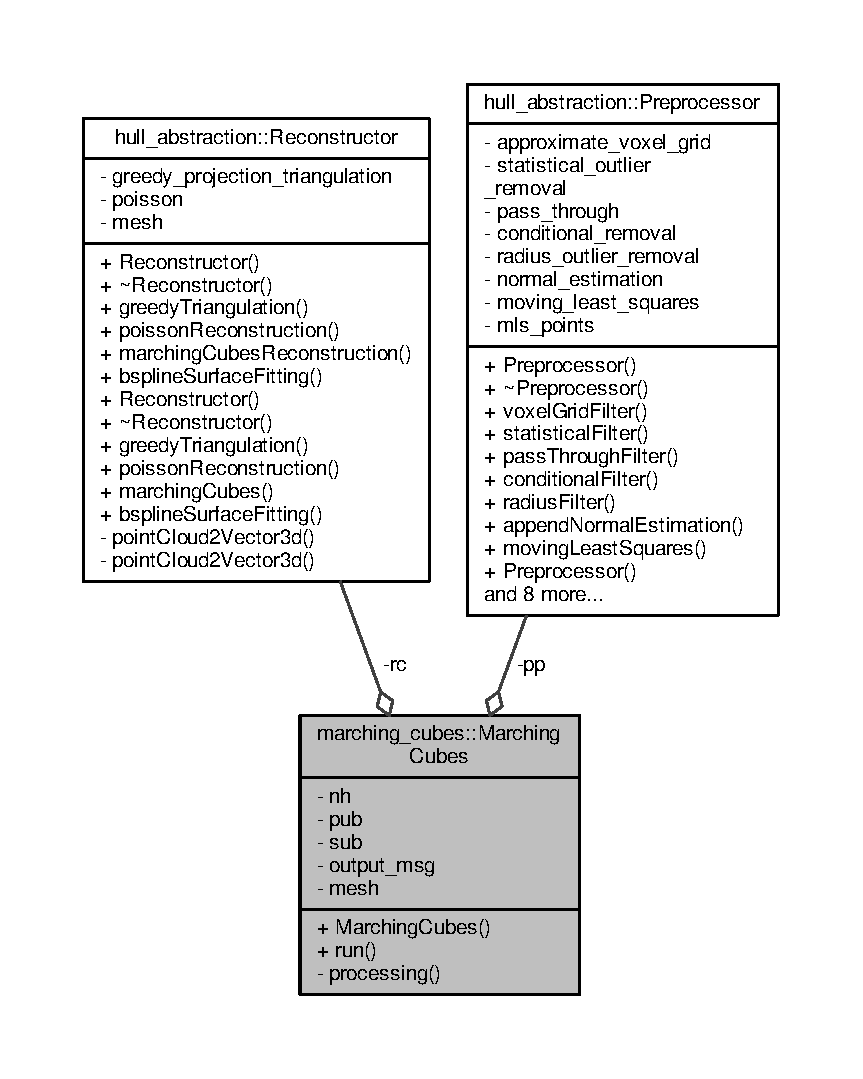
\includegraphics[width=350pt]{classmarching__cubes_1_1_marching_cubes__coll__graph}
\end{center}
\end{figure}
\subsection*{Public Member Functions}
\begin{DoxyCompactItemize}
\item 
\hyperlink{classmarching__cubes_1_1_marching_cubes_a1a953862541f2d2c6a3d6a5056c208b9}{Marching\+Cubes} ()
\begin{DoxyCompactList}\small\item\em Construct a new \hyperlink{classmarching__cubes_1_1_marching_cubes}{Marching\+Cubes} object. \end{DoxyCompactList}\item 
void \hyperlink{classmarching__cubes_1_1_marching_cubes_aad8747fa8bd083aa939873d98814966e}{run} ()
\begin{DoxyCompactList}\small\item\em Encapsulate a method to run the \hyperlink{namespacemarching__cubes}{marching\+\_\+cubes} node. \end{DoxyCompactList}\end{DoxyCompactItemize}
\subsection*{Private Member Functions}
\begin{DoxyCompactItemize}
\item 
void \hyperlink{classmarching__cubes_1_1_marching_cubes_a7d81fc975a0a768a175af838cd4fbc86}{processing} (const sensor\+\_\+msgs\+::\+Point\+Cloud2\+Const\+Ptr input\+\_\+msg)
\begin{DoxyCompactList}\small\item\em Process the point cloud message to create mesh message. \end{DoxyCompactList}\end{DoxyCompactItemize}
\subsection*{Private Attributes}
\begin{DoxyCompactItemize}
\item 
ros\+::\+Node\+Handle \hyperlink{classmarching__cubes_1_1_marching_cubes_a892881775be45a5cc1de7f19ca57e8d0}{nh}
\item 
ros\+::\+Publisher \hyperlink{classmarching__cubes_1_1_marching_cubes_afb0123959f5be68d13e50a77c0e6cd11}{pub}
\item 
ros\+::\+Subscriber \hyperlink{classmarching__cubes_1_1_marching_cubes_a7330eddbb78d73dc9aa809354985cee1}{sub}
\item 
pcl\+\_\+msgs\+::\+Polygon\+Mesh \hyperlink{classmarching__cubes_1_1_marching_cubes_a355aafbff47eae3e8ce9829a96c70f89}{output\+\_\+msg}
\item 
\hyperlink{classhull__abstraction_1_1_reconstructor}{hull\+\_\+abstraction\+::\+Reconstructor} \hyperlink{classmarching__cubes_1_1_marching_cubes_a80dcffe7ec661fb3fc85edbdebebc0db}{rc}
\item 
\hyperlink{classhull__abstraction_1_1_preprocessor}{hull\+\_\+abstraction\+::\+Preprocessor} \hyperlink{classmarching__cubes_1_1_marching_cubes_a72ffa2bde7429caf094e1e50b7e839dd}{pp}
\item 
pcl\+::\+Polygon\+Mesh \hyperlink{classmarching__cubes_1_1_marching_cubes_a169d75a95f59aa253a12d5322852f95d}{mesh}
\end{DoxyCompactItemize}


\subsection{Detailed Description}
Class utilizing marching cubes method. 

This framework is developed to generate a mesh for a point cloud through marching cubes methods. 

\subsection{Constructor \& Destructor Documentation}
\index{marching\+\_\+cubes\+::\+Marching\+Cubes@{marching\+\_\+cubes\+::\+Marching\+Cubes}!Marching\+Cubes@{Marching\+Cubes}}
\index{Marching\+Cubes@{Marching\+Cubes}!marching\+\_\+cubes\+::\+Marching\+Cubes@{marching\+\_\+cubes\+::\+Marching\+Cubes}}
\subsubsection[{\texorpdfstring{Marching\+Cubes()}{MarchingCubes()}}]{\setlength{\rightskip}{0pt plus 5cm}marching\+\_\+cubes\+::\+Marching\+Cubes\+::\+Marching\+Cubes (
\begin{DoxyParamCaption}
{}
\end{DoxyParamCaption}
)\hspace{0.3cm}{\ttfamily [inline]}}\hypertarget{classmarching__cubes_1_1_marching_cubes_a1a953862541f2d2c6a3d6a5056c208b9}{}\label{classmarching__cubes_1_1_marching_cubes_a1a953862541f2d2c6a3d6a5056c208b9}


Construct a new \hyperlink{classmarching__cubes_1_1_marching_cubes}{Marching\+Cubes} object. 



\subsection{Member Function Documentation}
\index{marching\+\_\+cubes\+::\+Marching\+Cubes@{marching\+\_\+cubes\+::\+Marching\+Cubes}!processing@{processing}}
\index{processing@{processing}!marching\+\_\+cubes\+::\+Marching\+Cubes@{marching\+\_\+cubes\+::\+Marching\+Cubes}}
\subsubsection[{\texorpdfstring{processing(const sensor\+\_\+msgs\+::\+Point\+Cloud2\+Const\+Ptr input\+\_\+msg)}{processing(const sensor_msgs::PointCloud2ConstPtr input_msg)}}]{\setlength{\rightskip}{0pt plus 5cm}void marching\+\_\+cubes\+::\+Marching\+Cubes\+::processing (
\begin{DoxyParamCaption}
\item[{const sensor\+\_\+msgs\+::\+Point\+Cloud2\+Const\+Ptr}]{input\+\_\+msg}
\end{DoxyParamCaption}
)\hspace{0.3cm}{\ttfamily [private]}}\hypertarget{classmarching__cubes_1_1_marching_cubes_a7d81fc975a0a768a175af838cd4fbc86}{}\label{classmarching__cubes_1_1_marching_cubes_a7d81fc975a0a768a175af838cd4fbc86}


Process the point cloud message to create mesh message. 


\begin{DoxyParams}{Parameters}
{\em input\+\_\+msg} & Input point cloud message \\
\hline
\end{DoxyParams}
\index{marching\+\_\+cubes\+::\+Marching\+Cubes@{marching\+\_\+cubes\+::\+Marching\+Cubes}!run@{run}}
\index{run@{run}!marching\+\_\+cubes\+::\+Marching\+Cubes@{marching\+\_\+cubes\+::\+Marching\+Cubes}}
\subsubsection[{\texorpdfstring{run()}{run()}}]{\setlength{\rightskip}{0pt plus 5cm}void marching\+\_\+cubes\+::\+Marching\+Cubes\+::run (
\begin{DoxyParamCaption}
{}
\end{DoxyParamCaption}
)}\hypertarget{classmarching__cubes_1_1_marching_cubes_aad8747fa8bd083aa939873d98814966e}{}\label{classmarching__cubes_1_1_marching_cubes_aad8747fa8bd083aa939873d98814966e}


Encapsulate a method to run the \hyperlink{namespacemarching__cubes}{marching\+\_\+cubes} node. 



\subsection{Member Data Documentation}
\index{marching\+\_\+cubes\+::\+Marching\+Cubes@{marching\+\_\+cubes\+::\+Marching\+Cubes}!mesh@{mesh}}
\index{mesh@{mesh}!marching\+\_\+cubes\+::\+Marching\+Cubes@{marching\+\_\+cubes\+::\+Marching\+Cubes}}
\subsubsection[{\texorpdfstring{mesh}{mesh}}]{\setlength{\rightskip}{0pt plus 5cm}pcl\+::\+Polygon\+Mesh marching\+\_\+cubes\+::\+Marching\+Cubes\+::mesh\hspace{0.3cm}{\ttfamily [private]}}\hypertarget{classmarching__cubes_1_1_marching_cubes_a169d75a95f59aa253a12d5322852f95d}{}\label{classmarching__cubes_1_1_marching_cubes_a169d75a95f59aa253a12d5322852f95d}
Resulted polygon mesh \index{marching\+\_\+cubes\+::\+Marching\+Cubes@{marching\+\_\+cubes\+::\+Marching\+Cubes}!nh@{nh}}
\index{nh@{nh}!marching\+\_\+cubes\+::\+Marching\+Cubes@{marching\+\_\+cubes\+::\+Marching\+Cubes}}
\subsubsection[{\texorpdfstring{nh}{nh}}]{\setlength{\rightskip}{0pt plus 5cm}ros\+::\+Node\+Handle marching\+\_\+cubes\+::\+Marching\+Cubes\+::nh\hspace{0.3cm}{\ttfamily [private]}}\hypertarget{classmarching__cubes_1_1_marching_cubes_a892881775be45a5cc1de7f19ca57e8d0}{}\label{classmarching__cubes_1_1_marching_cubes_a892881775be45a5cc1de7f19ca57e8d0}
Node Handle reference from embedding node \index{marching\+\_\+cubes\+::\+Marching\+Cubes@{marching\+\_\+cubes\+::\+Marching\+Cubes}!output\+\_\+msg@{output\+\_\+msg}}
\index{output\+\_\+msg@{output\+\_\+msg}!marching\+\_\+cubes\+::\+Marching\+Cubes@{marching\+\_\+cubes\+::\+Marching\+Cubes}}
\subsubsection[{\texorpdfstring{output\+\_\+msg}{output_msg}}]{\setlength{\rightskip}{0pt plus 5cm}pcl\+\_\+msgs\+::\+Polygon\+Mesh marching\+\_\+cubes\+::\+Marching\+Cubes\+::output\+\_\+msg\hspace{0.3cm}{\ttfamily [private]}}\hypertarget{classmarching__cubes_1_1_marching_cubes_a355aafbff47eae3e8ce9829a96c70f89}{}\label{classmarching__cubes_1_1_marching_cubes_a355aafbff47eae3e8ce9829a96c70f89}
Polygon mesh message used to publish the mesh \index{marching\+\_\+cubes\+::\+Marching\+Cubes@{marching\+\_\+cubes\+::\+Marching\+Cubes}!pp@{pp}}
\index{pp@{pp}!marching\+\_\+cubes\+::\+Marching\+Cubes@{marching\+\_\+cubes\+::\+Marching\+Cubes}}
\subsubsection[{\texorpdfstring{pp}{pp}}]{\setlength{\rightskip}{0pt plus 5cm}{\bf hull\+\_\+abstraction\+::\+Preprocessor} marching\+\_\+cubes\+::\+Marching\+Cubes\+::pp\hspace{0.3cm}{\ttfamily [private]}}\hypertarget{classmarching__cubes_1_1_marching_cubes_a72ffa2bde7429caf094e1e50b7e839dd}{}\label{classmarching__cubes_1_1_marching_cubes_a72ffa2bde7429caf094e1e50b7e839dd}
Object for Preprocessor class \index{marching\+\_\+cubes\+::\+Marching\+Cubes@{marching\+\_\+cubes\+::\+Marching\+Cubes}!pub@{pub}}
\index{pub@{pub}!marching\+\_\+cubes\+::\+Marching\+Cubes@{marching\+\_\+cubes\+::\+Marching\+Cubes}}
\subsubsection[{\texorpdfstring{pub}{pub}}]{\setlength{\rightskip}{0pt plus 5cm}ros\+::\+Publisher marching\+\_\+cubes\+::\+Marching\+Cubes\+::pub\hspace{0.3cm}{\ttfamily [private]}}\hypertarget{classmarching__cubes_1_1_marching_cubes_afb0123959f5be68d13e50a77c0e6cd11}{}\label{classmarching__cubes_1_1_marching_cubes_afb0123959f5be68d13e50a77c0e6cd11}
Polygon mesh publisher \index{marching\+\_\+cubes\+::\+Marching\+Cubes@{marching\+\_\+cubes\+::\+Marching\+Cubes}!rc@{rc}}
\index{rc@{rc}!marching\+\_\+cubes\+::\+Marching\+Cubes@{marching\+\_\+cubes\+::\+Marching\+Cubes}}
\subsubsection[{\texorpdfstring{rc}{rc}}]{\setlength{\rightskip}{0pt plus 5cm}{\bf hull\+\_\+abstraction\+::\+Reconstructor} marching\+\_\+cubes\+::\+Marching\+Cubes\+::rc\hspace{0.3cm}{\ttfamily [private]}}\hypertarget{classmarching__cubes_1_1_marching_cubes_a80dcffe7ec661fb3fc85edbdebebc0db}{}\label{classmarching__cubes_1_1_marching_cubes_a80dcffe7ec661fb3fc85edbdebebc0db}
Object for Reconstructor class \index{marching\+\_\+cubes\+::\+Marching\+Cubes@{marching\+\_\+cubes\+::\+Marching\+Cubes}!sub@{sub}}
\index{sub@{sub}!marching\+\_\+cubes\+::\+Marching\+Cubes@{marching\+\_\+cubes\+::\+Marching\+Cubes}}
\subsubsection[{\texorpdfstring{sub}{sub}}]{\setlength{\rightskip}{0pt plus 5cm}ros\+::\+Subscriber marching\+\_\+cubes\+::\+Marching\+Cubes\+::sub\hspace{0.3cm}{\ttfamily [private]}}\hypertarget{classmarching__cubes_1_1_marching_cubes_a7330eddbb78d73dc9aa809354985cee1}{}\label{classmarching__cubes_1_1_marching_cubes_a7330eddbb78d73dc9aa809354985cee1}
Raw point cloud subscriber 

The documentation for this class was generated from the following files\+:\begin{DoxyCompactItemize}
\item 
/home/jc/\+T\+H\+E\+S\+I\+S/hull\+\_\+abstraction/ros/src/hull\+\_\+abstraction/src/marching\+\_\+cubes\+\_\+node/\hyperlink{marching__cubes_8h}{marching\+\_\+cubes.\+h}\item 
/home/jc/\+T\+H\+E\+S\+I\+S/hull\+\_\+abstraction/ros/src/hull\+\_\+abstraction/src/marching\+\_\+cubes\+\_\+node/\hyperlink{marching__cubes_8cpp}{marching\+\_\+cubes.\+cpp}\end{DoxyCompactItemize}

\hypertarget{classmoving__least__squares__node_1_1_moving_least_squares}{}\section{moving\+\_\+least\+\_\+squares\+\_\+node\+:\+:Moving\+Least\+Squares Class Reference}
\label{classmoving__least__squares__node_1_1_moving_least_squares}\index{moving\+\_\+least\+\_\+squares\+\_\+node\+::\+Moving\+Least\+Squares@{moving\+\_\+least\+\_\+squares\+\_\+node\+::\+Moving\+Least\+Squares}}


Class utilizing moving least squares method.  




{\ttfamily \#include $<$moving\+\_\+least\+\_\+squares.\+h$>$}



Collaboration diagram for moving\+\_\+least\+\_\+squares\+\_\+node\+:\+:Moving\+Least\+Squares\+:\nopagebreak
\begin{figure}[H]
\begin{center}
\leavevmode
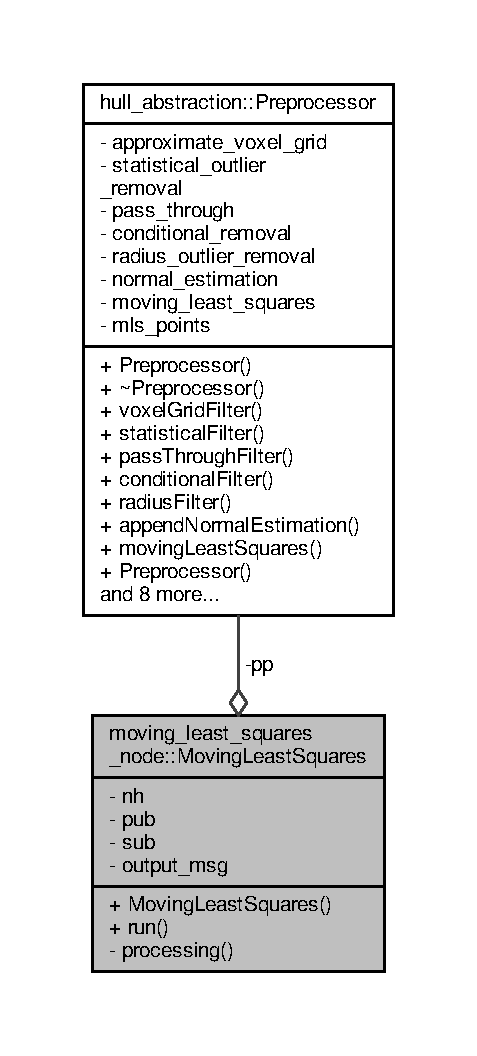
\includegraphics[width=229pt]{classmoving__least__squares__node_1_1_moving_least_squares__coll__graph}
\end{center}
\end{figure}
\subsection*{Public Member Functions}
\begin{DoxyCompactItemize}
\item 
\hyperlink{classmoving__least__squares__node_1_1_moving_least_squares_a55eba7b489543e53e018651e1039e51a}{Moving\+Least\+Squares} ()
\begin{DoxyCompactList}\small\item\em Construct a new \hyperlink{classmoving__least__squares__node_1_1_moving_least_squares}{Moving\+Least\+Squares} object. \end{DoxyCompactList}\item 
void \hyperlink{classmoving__least__squares__node_1_1_moving_least_squares_afb03a339aa9ae129d42af0b7d49dfb2c}{run} ()
\begin{DoxyCompactList}\small\item\em Encapsulate a method to run the moving\+\_\+least\+\_\+squares node. \end{DoxyCompactList}\end{DoxyCompactItemize}
\subsection*{Private Member Functions}
\begin{DoxyCompactItemize}
\item 
void \hyperlink{classmoving__least__squares__node_1_1_moving_least_squares_ab334356e26407324a4fb15ab3dbf9daa}{processing} (const sensor\+\_\+msgs\+::\+Point\+Cloud2\+Const\+Ptr input\+\_\+msg)
\begin{DoxyCompactList}\small\item\em Processing the input R\+OS message. \end{DoxyCompactList}\end{DoxyCompactItemize}
\subsection*{Private Attributes}
\begin{DoxyCompactItemize}
\item 
ros\+::\+Node\+Handle \hyperlink{classmoving__least__squares__node_1_1_moving_least_squares_ae4c2a5c0960cec2bc990d0f19fee3ecb}{nh}
\item 
ros\+::\+Publisher \hyperlink{classmoving__least__squares__node_1_1_moving_least_squares_a575c8db3fd78dc6e4bfd432d2d75916c}{pub}
\item 
ros\+::\+Subscriber \hyperlink{classmoving__least__squares__node_1_1_moving_least_squares_a3afb046b92a8d8df03d06542ba9fc9bd}{sub}
\item 
sensor\+\_\+msgs\+::\+Point\+Cloud2 \hyperlink{classmoving__least__squares__node_1_1_moving_least_squares_af6fbf84b91043961cc80fb71505992dd}{output\+\_\+msg}
\item 
\hyperlink{classhull__abstraction_1_1_preprocessor}{hull\+\_\+abstraction\+::\+Preprocessor} \hyperlink{classmoving__least__squares__node_1_1_moving_least_squares_a64551d7faad6e219620e142472edbada}{pp}
\end{DoxyCompactItemize}


\subsection{Detailed Description}
Class utilizing moving least squares method. 

This framework is developed to apply moving least squares method to smoothen the input point cloud. 

\subsection{Constructor \& Destructor Documentation}
\index{moving\+\_\+least\+\_\+squares\+\_\+node\+::\+Moving\+Least\+Squares@{moving\+\_\+least\+\_\+squares\+\_\+node\+::\+Moving\+Least\+Squares}!Moving\+Least\+Squares@{Moving\+Least\+Squares}}
\index{Moving\+Least\+Squares@{Moving\+Least\+Squares}!moving\+\_\+least\+\_\+squares\+\_\+node\+::\+Moving\+Least\+Squares@{moving\+\_\+least\+\_\+squares\+\_\+node\+::\+Moving\+Least\+Squares}}
\subsubsection[{\texorpdfstring{Moving\+Least\+Squares()}{MovingLeastSquares()}}]{\setlength{\rightskip}{0pt plus 5cm}moving\+\_\+least\+\_\+squares\+\_\+node\+::\+Moving\+Least\+Squares\+::\+Moving\+Least\+Squares (
\begin{DoxyParamCaption}
{}
\end{DoxyParamCaption}
)\hspace{0.3cm}{\ttfamily [inline]}}\hypertarget{classmoving__least__squares__node_1_1_moving_least_squares_a55eba7b489543e53e018651e1039e51a}{}\label{classmoving__least__squares__node_1_1_moving_least_squares_a55eba7b489543e53e018651e1039e51a}


Construct a new \hyperlink{classmoving__least__squares__node_1_1_moving_least_squares}{Moving\+Least\+Squares} object. 



\subsection{Member Function Documentation}
\index{moving\+\_\+least\+\_\+squares\+\_\+node\+::\+Moving\+Least\+Squares@{moving\+\_\+least\+\_\+squares\+\_\+node\+::\+Moving\+Least\+Squares}!processing@{processing}}
\index{processing@{processing}!moving\+\_\+least\+\_\+squares\+\_\+node\+::\+Moving\+Least\+Squares@{moving\+\_\+least\+\_\+squares\+\_\+node\+::\+Moving\+Least\+Squares}}
\subsubsection[{\texorpdfstring{processing(const sensor\+\_\+msgs\+::\+Point\+Cloud2\+Const\+Ptr input\+\_\+msg)}{processing(const sensor_msgs::PointCloud2ConstPtr input_msg)}}]{\setlength{\rightskip}{0pt plus 5cm}void moving\+\_\+least\+\_\+squares\+\_\+node\+::\+Moving\+Least\+Squares\+::processing (
\begin{DoxyParamCaption}
\item[{const sensor\+\_\+msgs\+::\+Point\+Cloud2\+Const\+Ptr}]{input\+\_\+msg}
\end{DoxyParamCaption}
)\hspace{0.3cm}{\ttfamily [private]}}\hypertarget{classmoving__least__squares__node_1_1_moving_least_squares_ab334356e26407324a4fb15ab3dbf9daa}{}\label{classmoving__least__squares__node_1_1_moving_least_squares_ab334356e26407324a4fb15ab3dbf9daa}


Processing the input R\+OS message. 


\begin{DoxyParams}{Parameters}
{\em input\+\_\+msg} & Input R\+OS message \\
\hline
\end{DoxyParams}
\index{moving\+\_\+least\+\_\+squares\+\_\+node\+::\+Moving\+Least\+Squares@{moving\+\_\+least\+\_\+squares\+\_\+node\+::\+Moving\+Least\+Squares}!run@{run}}
\index{run@{run}!moving\+\_\+least\+\_\+squares\+\_\+node\+::\+Moving\+Least\+Squares@{moving\+\_\+least\+\_\+squares\+\_\+node\+::\+Moving\+Least\+Squares}}
\subsubsection[{\texorpdfstring{run()}{run()}}]{\setlength{\rightskip}{0pt plus 5cm}void moving\+\_\+least\+\_\+squares\+\_\+node\+::\+Moving\+Least\+Squares\+::run (
\begin{DoxyParamCaption}
{}
\end{DoxyParamCaption}
)}\hypertarget{classmoving__least__squares__node_1_1_moving_least_squares_afb03a339aa9ae129d42af0b7d49dfb2c}{}\label{classmoving__least__squares__node_1_1_moving_least_squares_afb03a339aa9ae129d42af0b7d49dfb2c}


Encapsulate a method to run the moving\+\_\+least\+\_\+squares node. 



\subsection{Member Data Documentation}
\index{moving\+\_\+least\+\_\+squares\+\_\+node\+::\+Moving\+Least\+Squares@{moving\+\_\+least\+\_\+squares\+\_\+node\+::\+Moving\+Least\+Squares}!nh@{nh}}
\index{nh@{nh}!moving\+\_\+least\+\_\+squares\+\_\+node\+::\+Moving\+Least\+Squares@{moving\+\_\+least\+\_\+squares\+\_\+node\+::\+Moving\+Least\+Squares}}
\subsubsection[{\texorpdfstring{nh}{nh}}]{\setlength{\rightskip}{0pt plus 5cm}ros\+::\+Node\+Handle moving\+\_\+least\+\_\+squares\+\_\+node\+::\+Moving\+Least\+Squares\+::nh\hspace{0.3cm}{\ttfamily [private]}}\hypertarget{classmoving__least__squares__node_1_1_moving_least_squares_ae4c2a5c0960cec2bc990d0f19fee3ecb}{}\label{classmoving__least__squares__node_1_1_moving_least_squares_ae4c2a5c0960cec2bc990d0f19fee3ecb}
Node Handle reference from embedding node \index{moving\+\_\+least\+\_\+squares\+\_\+node\+::\+Moving\+Least\+Squares@{moving\+\_\+least\+\_\+squares\+\_\+node\+::\+Moving\+Least\+Squares}!output\+\_\+msg@{output\+\_\+msg}}
\index{output\+\_\+msg@{output\+\_\+msg}!moving\+\_\+least\+\_\+squares\+\_\+node\+::\+Moving\+Least\+Squares@{moving\+\_\+least\+\_\+squares\+\_\+node\+::\+Moving\+Least\+Squares}}
\subsubsection[{\texorpdfstring{output\+\_\+msg}{output_msg}}]{\setlength{\rightskip}{0pt plus 5cm}sensor\+\_\+msgs\+::\+Point\+Cloud2 moving\+\_\+least\+\_\+squares\+\_\+node\+::\+Moving\+Least\+Squares\+::output\+\_\+msg\hspace{0.3cm}{\ttfamily [private]}}\hypertarget{classmoving__least__squares__node_1_1_moving_least_squares_af6fbf84b91043961cc80fb71505992dd}{}\label{classmoving__least__squares__node_1_1_moving_least_squares_af6fbf84b91043961cc80fb71505992dd}
point cloud message used to publish the result \index{moving\+\_\+least\+\_\+squares\+\_\+node\+::\+Moving\+Least\+Squares@{moving\+\_\+least\+\_\+squares\+\_\+node\+::\+Moving\+Least\+Squares}!pp@{pp}}
\index{pp@{pp}!moving\+\_\+least\+\_\+squares\+\_\+node\+::\+Moving\+Least\+Squares@{moving\+\_\+least\+\_\+squares\+\_\+node\+::\+Moving\+Least\+Squares}}
\subsubsection[{\texorpdfstring{pp}{pp}}]{\setlength{\rightskip}{0pt plus 5cm}{\bf hull\+\_\+abstraction\+::\+Preprocessor} moving\+\_\+least\+\_\+squares\+\_\+node\+::\+Moving\+Least\+Squares\+::pp\hspace{0.3cm}{\ttfamily [private]}}\hypertarget{classmoving__least__squares__node_1_1_moving_least_squares_a64551d7faad6e219620e142472edbada}{}\label{classmoving__least__squares__node_1_1_moving_least_squares_a64551d7faad6e219620e142472edbada}
Object for Preprocessor class \index{moving\+\_\+least\+\_\+squares\+\_\+node\+::\+Moving\+Least\+Squares@{moving\+\_\+least\+\_\+squares\+\_\+node\+::\+Moving\+Least\+Squares}!pub@{pub}}
\index{pub@{pub}!moving\+\_\+least\+\_\+squares\+\_\+node\+::\+Moving\+Least\+Squares@{moving\+\_\+least\+\_\+squares\+\_\+node\+::\+Moving\+Least\+Squares}}
\subsubsection[{\texorpdfstring{pub}{pub}}]{\setlength{\rightskip}{0pt plus 5cm}ros\+::\+Publisher moving\+\_\+least\+\_\+squares\+\_\+node\+::\+Moving\+Least\+Squares\+::pub\hspace{0.3cm}{\ttfamily [private]}}\hypertarget{classmoving__least__squares__node_1_1_moving_least_squares_a575c8db3fd78dc6e4bfd432d2d75916c}{}\label{classmoving__least__squares__node_1_1_moving_least_squares_a575c8db3fd78dc6e4bfd432d2d75916c}
Point cloud publisher \index{moving\+\_\+least\+\_\+squares\+\_\+node\+::\+Moving\+Least\+Squares@{moving\+\_\+least\+\_\+squares\+\_\+node\+::\+Moving\+Least\+Squares}!sub@{sub}}
\index{sub@{sub}!moving\+\_\+least\+\_\+squares\+\_\+node\+::\+Moving\+Least\+Squares@{moving\+\_\+least\+\_\+squares\+\_\+node\+::\+Moving\+Least\+Squares}}
\subsubsection[{\texorpdfstring{sub}{sub}}]{\setlength{\rightskip}{0pt plus 5cm}ros\+::\+Subscriber moving\+\_\+least\+\_\+squares\+\_\+node\+::\+Moving\+Least\+Squares\+::sub\hspace{0.3cm}{\ttfamily [private]}}\hypertarget{classmoving__least__squares__node_1_1_moving_least_squares_a3afb046b92a8d8df03d06542ba9fc9bd}{}\label{classmoving__least__squares__node_1_1_moving_least_squares_a3afb046b92a8d8df03d06542ba9fc9bd}
Raw point cloud subscriber 

The documentation for this class was generated from the following files\+:\begin{DoxyCompactItemize}
\item 
/home/jc/hull\+\_\+abstraction/ros/src/hull\+\_\+abstraction/src/moving\+\_\+least\+\_\+squares\+\_\+node/\hyperlink{moving__least__squares_8h}{moving\+\_\+least\+\_\+squares.\+h}\item 
/home/jc/hull\+\_\+abstraction/ros/src/hull\+\_\+abstraction/src/moving\+\_\+least\+\_\+squares\+\_\+node/\hyperlink{moving__least__squares_8cpp}{moving\+\_\+least\+\_\+squares.\+cpp}\end{DoxyCompactItemize}

\hypertarget{classpoisson__reconstruction_1_1_poisson_reconstruction}{}\section{poisson\+\_\+reconstruction\+:\+:Poisson\+Reconstruction Class Reference}
\label{classpoisson__reconstruction_1_1_poisson_reconstruction}\index{poisson\+\_\+reconstruction\+::\+Poisson\+Reconstruction@{poisson\+\_\+reconstruction\+::\+Poisson\+Reconstruction}}


Class utilizing Poisson reconstruction method.  




{\ttfamily \#include $<$poisson\+\_\+reconstruction.\+h$>$}



Collaboration diagram for poisson\+\_\+reconstruction\+:\+:Poisson\+Reconstruction\+:
\nopagebreak
\begin{figure}[H]
\begin{center}
\leavevmode
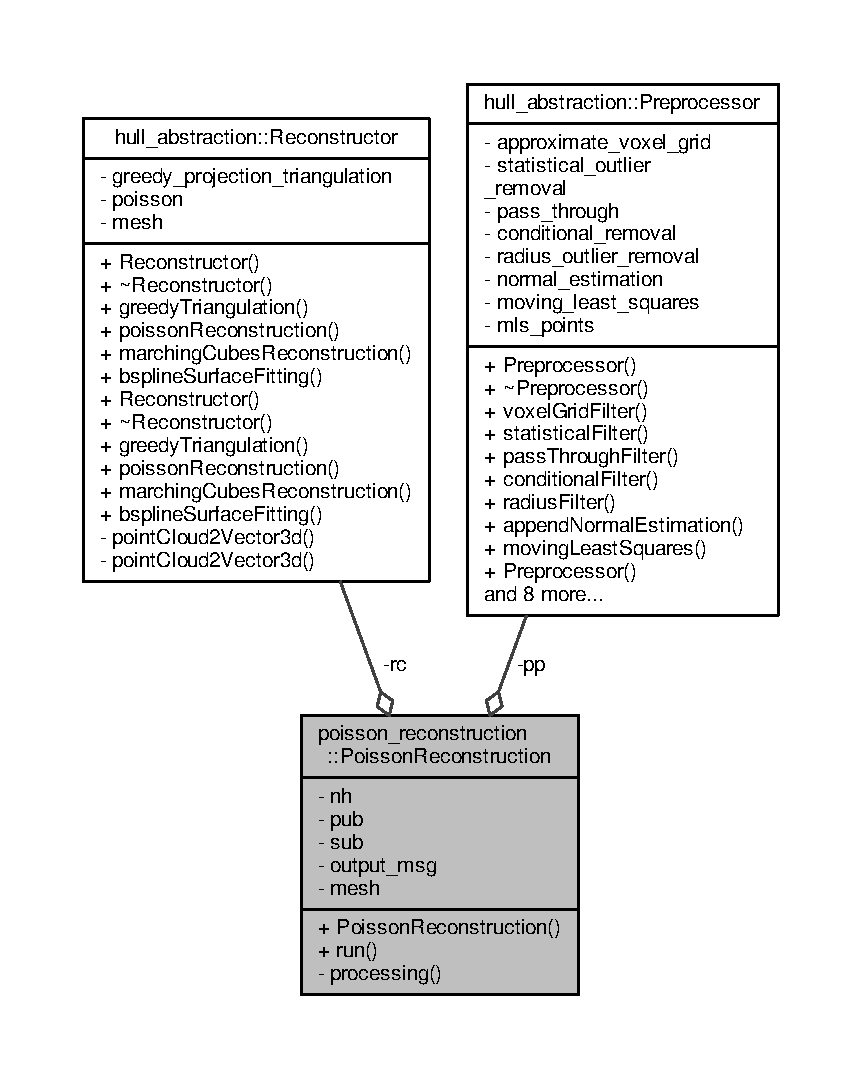
\includegraphics[width=350pt]{classpoisson__reconstruction_1_1_poisson_reconstruction__coll__graph}
\end{center}
\end{figure}
\subsection*{Public Member Functions}
\begin{DoxyCompactItemize}
\item 
\hyperlink{classpoisson__reconstruction_1_1_poisson_reconstruction_a90460dde9c30757ccb95052e65cf58ef}{Poisson\+Reconstruction} ()
\begin{DoxyCompactList}\small\item\em Construct a new \hyperlink{classpoisson__reconstruction_1_1_poisson_reconstruction}{Poisson\+Reconstruction} object. \end{DoxyCompactList}\item 
void \hyperlink{classpoisson__reconstruction_1_1_poisson_reconstruction_aa8ff149207e40459c6443041798df811}{run} ()
\begin{DoxyCompactList}\small\item\em Encapsulate a method to run the \hyperlink{namespacepoisson__reconstruction}{poisson\+\_\+reconstruction} node. \end{DoxyCompactList}\end{DoxyCompactItemize}
\subsection*{Private Member Functions}
\begin{DoxyCompactItemize}
\item 
void \hyperlink{classpoisson__reconstruction_1_1_poisson_reconstruction_a13eaff655ebb89b9e9dfdb56f11fed07}{processing} (const sensor\+\_\+msgs\+::\+Point\+Cloud2\+Const\+Ptr input\+\_\+msg)
\begin{DoxyCompactList}\small\item\em Process the point cloud message to create mesh message. \end{DoxyCompactList}\end{DoxyCompactItemize}
\subsection*{Private Attributes}
\begin{DoxyCompactItemize}
\item 
ros\+::\+Node\+Handle \hyperlink{classpoisson__reconstruction_1_1_poisson_reconstruction_ac18f4bd8c54335edb4c9154eed871ba5}{nh}
\item 
ros\+::\+Publisher \hyperlink{classpoisson__reconstruction_1_1_poisson_reconstruction_ad327638b4ca620ad0eebc8c9ba2f0dc5}{pub}
\item 
ros\+::\+Subscriber \hyperlink{classpoisson__reconstruction_1_1_poisson_reconstruction_a35abf57328b8f673fa0d0631378d8f19}{sub}
\item 
pcl\+\_\+msgs\+::\+Polygon\+Mesh \hyperlink{classpoisson__reconstruction_1_1_poisson_reconstruction_a10b2bb1e30658337e0780210acda450c}{output\+\_\+msg}
\item 
\hyperlink{classhull__abstraction_1_1_reconstructor}{hull\+\_\+abstraction\+::\+Reconstructor} \hyperlink{classpoisson__reconstruction_1_1_poisson_reconstruction_a2afb3b38fc52d7d8a0ef3e9a4d65027b}{rc}
\item 
\hyperlink{classhull__abstraction_1_1_preprocessor}{hull\+\_\+abstraction\+::\+Preprocessor} \hyperlink{classpoisson__reconstruction_1_1_poisson_reconstruction_a9229da88237b26a663a94c1aca3ceb52}{pp}
\item 
pcl\+::\+Polygon\+Mesh \hyperlink{classpoisson__reconstruction_1_1_poisson_reconstruction_a5815143b0a1d9bb5cbeeddff37564011}{mesh}
\end{DoxyCompactItemize}


\subsection{Detailed Description}
Class utilizing Poisson reconstruction method. 

This framework is developed to apply Poisson reconstruction to generate mesh based on the input point cloud. 

\subsection{Constructor \& Destructor Documentation}
\index{poisson\+\_\+reconstruction\+::\+Poisson\+Reconstruction@{poisson\+\_\+reconstruction\+::\+Poisson\+Reconstruction}!Poisson\+Reconstruction@{Poisson\+Reconstruction}}
\index{Poisson\+Reconstruction@{Poisson\+Reconstruction}!poisson\+\_\+reconstruction\+::\+Poisson\+Reconstruction@{poisson\+\_\+reconstruction\+::\+Poisson\+Reconstruction}}
\subsubsection[{\texorpdfstring{Poisson\+Reconstruction()}{PoissonReconstruction()}}]{\setlength{\rightskip}{0pt plus 5cm}poisson\+\_\+reconstruction\+::\+Poisson\+Reconstruction\+::\+Poisson\+Reconstruction (
\begin{DoxyParamCaption}
{}
\end{DoxyParamCaption}
)\hspace{0.3cm}{\ttfamily [inline]}}\hypertarget{classpoisson__reconstruction_1_1_poisson_reconstruction_a90460dde9c30757ccb95052e65cf58ef}{}\label{classpoisson__reconstruction_1_1_poisson_reconstruction_a90460dde9c30757ccb95052e65cf58ef}


Construct a new \hyperlink{classpoisson__reconstruction_1_1_poisson_reconstruction}{Poisson\+Reconstruction} object. 



\subsection{Member Function Documentation}
\index{poisson\+\_\+reconstruction\+::\+Poisson\+Reconstruction@{poisson\+\_\+reconstruction\+::\+Poisson\+Reconstruction}!processing@{processing}}
\index{processing@{processing}!poisson\+\_\+reconstruction\+::\+Poisson\+Reconstruction@{poisson\+\_\+reconstruction\+::\+Poisson\+Reconstruction}}
\subsubsection[{\texorpdfstring{processing(const sensor\+\_\+msgs\+::\+Point\+Cloud2\+Const\+Ptr input\+\_\+msg)}{processing(const sensor_msgs::PointCloud2ConstPtr input_msg)}}]{\setlength{\rightskip}{0pt plus 5cm}void poisson\+\_\+reconstruction\+::\+Poisson\+Reconstruction\+::processing (
\begin{DoxyParamCaption}
\item[{const sensor\+\_\+msgs\+::\+Point\+Cloud2\+Const\+Ptr}]{input\+\_\+msg}
\end{DoxyParamCaption}
)\hspace{0.3cm}{\ttfamily [private]}}\hypertarget{classpoisson__reconstruction_1_1_poisson_reconstruction_a13eaff655ebb89b9e9dfdb56f11fed07}{}\label{classpoisson__reconstruction_1_1_poisson_reconstruction_a13eaff655ebb89b9e9dfdb56f11fed07}


Process the point cloud message to create mesh message. 


\begin{DoxyParams}{Parameters}
{\em input\+\_\+msg} & Input point cloud message \\
\hline
\end{DoxyParams}
\index{poisson\+\_\+reconstruction\+::\+Poisson\+Reconstruction@{poisson\+\_\+reconstruction\+::\+Poisson\+Reconstruction}!run@{run}}
\index{run@{run}!poisson\+\_\+reconstruction\+::\+Poisson\+Reconstruction@{poisson\+\_\+reconstruction\+::\+Poisson\+Reconstruction}}
\subsubsection[{\texorpdfstring{run()}{run()}}]{\setlength{\rightskip}{0pt plus 5cm}void poisson\+\_\+reconstruction\+::\+Poisson\+Reconstruction\+::run (
\begin{DoxyParamCaption}
{}
\end{DoxyParamCaption}
)}\hypertarget{classpoisson__reconstruction_1_1_poisson_reconstruction_aa8ff149207e40459c6443041798df811}{}\label{classpoisson__reconstruction_1_1_poisson_reconstruction_aa8ff149207e40459c6443041798df811}


Encapsulate a method to run the \hyperlink{namespacepoisson__reconstruction}{poisson\+\_\+reconstruction} node. 



\subsection{Member Data Documentation}
\index{poisson\+\_\+reconstruction\+::\+Poisson\+Reconstruction@{poisson\+\_\+reconstruction\+::\+Poisson\+Reconstruction}!mesh@{mesh}}
\index{mesh@{mesh}!poisson\+\_\+reconstruction\+::\+Poisson\+Reconstruction@{poisson\+\_\+reconstruction\+::\+Poisson\+Reconstruction}}
\subsubsection[{\texorpdfstring{mesh}{mesh}}]{\setlength{\rightskip}{0pt plus 5cm}pcl\+::\+Polygon\+Mesh poisson\+\_\+reconstruction\+::\+Poisson\+Reconstruction\+::mesh\hspace{0.3cm}{\ttfamily [private]}}\hypertarget{classpoisson__reconstruction_1_1_poisson_reconstruction_a5815143b0a1d9bb5cbeeddff37564011}{}\label{classpoisson__reconstruction_1_1_poisson_reconstruction_a5815143b0a1d9bb5cbeeddff37564011}
Resulted polygon mesh \index{poisson\+\_\+reconstruction\+::\+Poisson\+Reconstruction@{poisson\+\_\+reconstruction\+::\+Poisson\+Reconstruction}!nh@{nh}}
\index{nh@{nh}!poisson\+\_\+reconstruction\+::\+Poisson\+Reconstruction@{poisson\+\_\+reconstruction\+::\+Poisson\+Reconstruction}}
\subsubsection[{\texorpdfstring{nh}{nh}}]{\setlength{\rightskip}{0pt plus 5cm}ros\+::\+Node\+Handle poisson\+\_\+reconstruction\+::\+Poisson\+Reconstruction\+::nh\hspace{0.3cm}{\ttfamily [private]}}\hypertarget{classpoisson__reconstruction_1_1_poisson_reconstruction_ac18f4bd8c54335edb4c9154eed871ba5}{}\label{classpoisson__reconstruction_1_1_poisson_reconstruction_ac18f4bd8c54335edb4c9154eed871ba5}
Node Handle reference from embedding node \index{poisson\+\_\+reconstruction\+::\+Poisson\+Reconstruction@{poisson\+\_\+reconstruction\+::\+Poisson\+Reconstruction}!output\+\_\+msg@{output\+\_\+msg}}
\index{output\+\_\+msg@{output\+\_\+msg}!poisson\+\_\+reconstruction\+::\+Poisson\+Reconstruction@{poisson\+\_\+reconstruction\+::\+Poisson\+Reconstruction}}
\subsubsection[{\texorpdfstring{output\+\_\+msg}{output_msg}}]{\setlength{\rightskip}{0pt plus 5cm}pcl\+\_\+msgs\+::\+Polygon\+Mesh poisson\+\_\+reconstruction\+::\+Poisson\+Reconstruction\+::output\+\_\+msg\hspace{0.3cm}{\ttfamily [private]}}\hypertarget{classpoisson__reconstruction_1_1_poisson_reconstruction_a10b2bb1e30658337e0780210acda450c}{}\label{classpoisson__reconstruction_1_1_poisson_reconstruction_a10b2bb1e30658337e0780210acda450c}
Polygon mesh message used to publish the mesh \index{poisson\+\_\+reconstruction\+::\+Poisson\+Reconstruction@{poisson\+\_\+reconstruction\+::\+Poisson\+Reconstruction}!pp@{pp}}
\index{pp@{pp}!poisson\+\_\+reconstruction\+::\+Poisson\+Reconstruction@{poisson\+\_\+reconstruction\+::\+Poisson\+Reconstruction}}
\subsubsection[{\texorpdfstring{pp}{pp}}]{\setlength{\rightskip}{0pt plus 5cm}{\bf hull\+\_\+abstraction\+::\+Preprocessor} poisson\+\_\+reconstruction\+::\+Poisson\+Reconstruction\+::pp\hspace{0.3cm}{\ttfamily [private]}}\hypertarget{classpoisson__reconstruction_1_1_poisson_reconstruction_a9229da88237b26a663a94c1aca3ceb52}{}\label{classpoisson__reconstruction_1_1_poisson_reconstruction_a9229da88237b26a663a94c1aca3ceb52}
Object for Preprocessor class \index{poisson\+\_\+reconstruction\+::\+Poisson\+Reconstruction@{poisson\+\_\+reconstruction\+::\+Poisson\+Reconstruction}!pub@{pub}}
\index{pub@{pub}!poisson\+\_\+reconstruction\+::\+Poisson\+Reconstruction@{poisson\+\_\+reconstruction\+::\+Poisson\+Reconstruction}}
\subsubsection[{\texorpdfstring{pub}{pub}}]{\setlength{\rightskip}{0pt plus 5cm}ros\+::\+Publisher poisson\+\_\+reconstruction\+::\+Poisson\+Reconstruction\+::pub\hspace{0.3cm}{\ttfamily [private]}}\hypertarget{classpoisson__reconstruction_1_1_poisson_reconstruction_ad327638b4ca620ad0eebc8c9ba2f0dc5}{}\label{classpoisson__reconstruction_1_1_poisson_reconstruction_ad327638b4ca620ad0eebc8c9ba2f0dc5}
Polygon mesh publisher \index{poisson\+\_\+reconstruction\+::\+Poisson\+Reconstruction@{poisson\+\_\+reconstruction\+::\+Poisson\+Reconstruction}!rc@{rc}}
\index{rc@{rc}!poisson\+\_\+reconstruction\+::\+Poisson\+Reconstruction@{poisson\+\_\+reconstruction\+::\+Poisson\+Reconstruction}}
\subsubsection[{\texorpdfstring{rc}{rc}}]{\setlength{\rightskip}{0pt plus 5cm}{\bf hull\+\_\+abstraction\+::\+Reconstructor} poisson\+\_\+reconstruction\+::\+Poisson\+Reconstruction\+::rc\hspace{0.3cm}{\ttfamily [private]}}\hypertarget{classpoisson__reconstruction_1_1_poisson_reconstruction_a2afb3b38fc52d7d8a0ef3e9a4d65027b}{}\label{classpoisson__reconstruction_1_1_poisson_reconstruction_a2afb3b38fc52d7d8a0ef3e9a4d65027b}
Object for Reconstructor class \index{poisson\+\_\+reconstruction\+::\+Poisson\+Reconstruction@{poisson\+\_\+reconstruction\+::\+Poisson\+Reconstruction}!sub@{sub}}
\index{sub@{sub}!poisson\+\_\+reconstruction\+::\+Poisson\+Reconstruction@{poisson\+\_\+reconstruction\+::\+Poisson\+Reconstruction}}
\subsubsection[{\texorpdfstring{sub}{sub}}]{\setlength{\rightskip}{0pt plus 5cm}ros\+::\+Subscriber poisson\+\_\+reconstruction\+::\+Poisson\+Reconstruction\+::sub\hspace{0.3cm}{\ttfamily [private]}}\hypertarget{classpoisson__reconstruction_1_1_poisson_reconstruction_a35abf57328b8f673fa0d0631378d8f19}{}\label{classpoisson__reconstruction_1_1_poisson_reconstruction_a35abf57328b8f673fa0d0631378d8f19}
Raw point cloud subscriber 

The documentation for this class was generated from the following files\+:\begin{DoxyCompactItemize}
\item 
/home/jc/hull\+\_\+abstraction/ros/src/hull\+\_\+abstraction/src/poisson\+\_\+reconstruction\+\_\+node/\hyperlink{poisson__reconstruction_8h}{poisson\+\_\+reconstruction.\+h}\item 
/home/jc/hull\+\_\+abstraction/ros/src/hull\+\_\+abstraction/src/poisson\+\_\+reconstruction\+\_\+node/\hyperlink{poisson__reconstruction_8cpp}{poisson\+\_\+reconstruction.\+cpp}\end{DoxyCompactItemize}

\hypertarget{classhull__abstraction_1_1_preprocessor}{}\section{hull\+\_\+abstraction\+:\+:Preprocessor Class Reference}
\label{classhull__abstraction_1_1_preprocessor}\index{hull\+\_\+abstraction\+::\+Preprocessor@{hull\+\_\+abstraction\+::\+Preprocessor}}


Class containing several preprocessing procedures.  




{\ttfamily \#include $<$preprocessor.\+h$>$}



Collaboration diagram for hull\+\_\+abstraction\+:\+:Preprocessor\+:\nopagebreak
\begin{figure}[H]
\begin{center}
\leavevmode
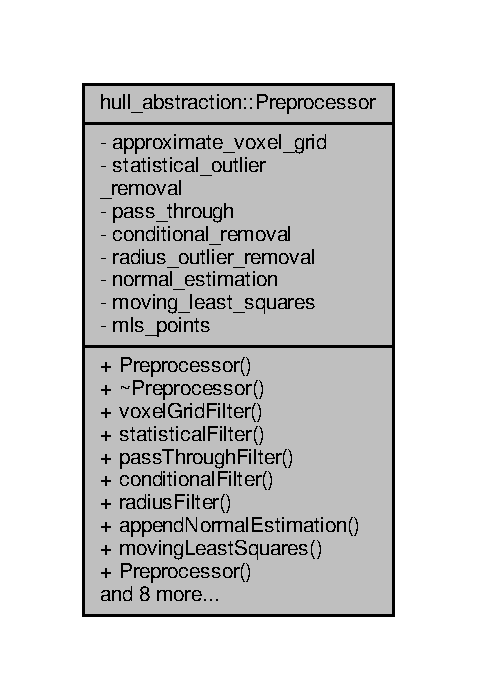
\includegraphics[width=229pt]{classhull__abstraction_1_1_preprocessor__coll__graph}
\end{center}
\end{figure}
\subsection*{Public Member Functions}
\begin{DoxyCompactItemize}
\item 
\hyperlink{classhull__abstraction_1_1_preprocessor_aa1e7b3418d273ceddd2faa0777f3598c}{Preprocessor} ()
\item 
\hyperlink{classhull__abstraction_1_1_preprocessor_a880dfe2a68232c6aea2ad41743df3d97}{$\sim$\+Preprocessor} ()
\item 
void \hyperlink{classhull__abstraction_1_1_preprocessor_a423d6c8cb5b08f8387290aae47184b3b}{voxel\+Grid\+Filter} (pcl\+::\+Point\+Cloud$<$ pcl\+::\+Point\+X\+YZ $>$\+::Ptr cloud, pcl\+::\+Point\+Cloud$<$ pcl\+::\+Point\+X\+YZ $>$\+::Ptr filtered\+\_\+cloud)
\item 
void \hyperlink{classhull__abstraction_1_1_preprocessor_a494877684eca0eaf7207c8655140b692}{statistical\+Filter} (pcl\+::\+Point\+Cloud$<$ pcl\+::\+Point\+X\+YZ $>$\+::Ptr cloud, pcl\+::\+Point\+Cloud$<$ pcl\+::\+Point\+X\+YZ $>$\+::Ptr filtered\+\_\+cloud)
\item 
void \hyperlink{classhull__abstraction_1_1_preprocessor_a4912126b50bdac35c63f521e3bc04314}{pass\+Through\+Filter} (pcl\+::\+Point\+Cloud$<$ pcl\+::\+Point\+X\+YZ $>$\+::Ptr cloud, pcl\+::\+Point\+Cloud$<$ pcl\+::\+Point\+X\+YZ $>$\+::Ptr filtered\+\_\+cloud)
\item 
void \hyperlink{classhull__abstraction_1_1_preprocessor_a95229af873f6f1a74c832340f8f9b7bf}{conditional\+Filter} (pcl\+::\+Point\+Cloud$<$ pcl\+::\+Point\+X\+YZ $>$\+::Ptr cloud, pcl\+::\+Point\+Cloud$<$ pcl\+::\+Point\+X\+YZ $>$\+::Ptr filtered\+\_\+cloud)
\item 
void \hyperlink{classhull__abstraction_1_1_preprocessor_aef6ccdc23a770af04eb6fc1d34aceff9}{radius\+Filter} (pcl\+::\+Point\+Cloud$<$ pcl\+::\+Point\+X\+YZ $>$\+::Ptr cloud, pcl\+::\+Point\+Cloud$<$ pcl\+::\+Point\+X\+YZ $>$\+::Ptr filtered\+\_\+cloud)
\item 
void \hyperlink{classhull__abstraction_1_1_preprocessor_a9768f4de4320607118636323343b5b5c}{append\+Normal\+Estimation} (pcl\+::\+Point\+Cloud$<$ pcl\+::\+Point\+X\+YZ $>$\+::Ptr cloud, pcl\+::\+Point\+Cloud$<$ pcl\+::\+Point\+Normal $>$\+::Ptr cloud\+\_\+with\+\_\+normals)
\item 
void \hyperlink{classhull__abstraction_1_1_preprocessor_adb771d9dfac554a7dd35db7d9acc3ca3}{moving\+Least\+Squares} (pcl\+::\+Point\+Cloud$<$ pcl\+::\+Point\+X\+YZ $>$\+::Ptr cloud, pcl\+::\+Point\+Cloud$<$ pcl\+::\+Point\+X\+YZ $>$\+::Ptr smoothed\+\_\+cloud, pcl\+::\+Point\+Cloud$<$ pcl\+::\+Point\+Normal $>$\+::Ptr smoothed\+\_\+cloud\+\_\+with\+\_\+normals)
\item 
\hyperlink{classhull__abstraction_1_1_preprocessor_aa1e7b3418d273ceddd2faa0777f3598c}{Preprocessor} ()
\begin{DoxyCompactList}\small\item\em Construct a new \hyperlink{classhull__abstraction_1_1_preprocessor}{Preprocessor} object. \end{DoxyCompactList}\item 
\hyperlink{classhull__abstraction_1_1_preprocessor_a880dfe2a68232c6aea2ad41743df3d97}{$\sim$\+Preprocessor} ()
\begin{DoxyCompactList}\small\item\em Destroy the \hyperlink{classhull__abstraction_1_1_preprocessor}{Preprocessor} object. \end{DoxyCompactList}\item 
void \hyperlink{classhull__abstraction_1_1_preprocessor_a423d6c8cb5b08f8387290aae47184b3b}{voxel\+Grid\+Filter} (pcl\+::\+Point\+Cloud$<$ pcl\+::\+Point\+X\+YZ $>$\+::Ptr cloud, pcl\+::\+Point\+Cloud$<$ pcl\+::\+Point\+X\+YZ $>$\+::Ptr filtered\+\_\+cloud)
\begin{DoxyCompactList}\small\item\em Implementation of the voxel grid filter to perform down sampling. \end{DoxyCompactList}\item 
void \hyperlink{classhull__abstraction_1_1_preprocessor_a494877684eca0eaf7207c8655140b692}{statistical\+Filter} (pcl\+::\+Point\+Cloud$<$ pcl\+::\+Point\+X\+YZ $>$\+::Ptr cloud, pcl\+::\+Point\+Cloud$<$ pcl\+::\+Point\+X\+YZ $>$\+::Ptr filtered\+\_\+cloud)
\begin{DoxyCompactList}\small\item\em Remove outliers through the statitical filter. \end{DoxyCompactList}\item 
void \hyperlink{classhull__abstraction_1_1_preprocessor_a4912126b50bdac35c63f521e3bc04314}{pass\+Through\+Filter} (pcl\+::\+Point\+Cloud$<$ pcl\+::\+Point\+X\+YZ $>$\+::Ptr cloud, pcl\+::\+Point\+Cloud$<$ pcl\+::\+Point\+X\+YZ $>$\+::Ptr filtered\+\_\+cloud)
\begin{DoxyCompactList}\small\item\em Implement the pass-\/through filter. \end{DoxyCompactList}\item 
void \hyperlink{classhull__abstraction_1_1_preprocessor_a95229af873f6f1a74c832340f8f9b7bf}{conditional\+Filter} (pcl\+::\+Point\+Cloud$<$ pcl\+::\+Point\+X\+YZ $>$\+::Ptr cloud, pcl\+::\+Point\+Cloud$<$ pcl\+::\+Point\+X\+YZ $>$\+::Ptr filtered\+\_\+cloud)
\begin{DoxyCompactList}\small\item\em Implement the conditional filter. \end{DoxyCompactList}\item 
void \hyperlink{classhull__abstraction_1_1_preprocessor_aef6ccdc23a770af04eb6fc1d34aceff9}{radius\+Filter} (pcl\+::\+Point\+Cloud$<$ pcl\+::\+Point\+X\+YZ $>$\+::Ptr cloud, pcl\+::\+Point\+Cloud$<$ pcl\+::\+Point\+X\+YZ $>$\+::Ptr filtered\+\_\+cloud)
\begin{DoxyCompactList}\small\item\em Implement the radius filter. \end{DoxyCompactList}\item 
void \hyperlink{classhull__abstraction_1_1_preprocessor_a9768f4de4320607118636323343b5b5c}{append\+Normal\+Estimation} (pcl\+::\+Point\+Cloud$<$ pcl\+::\+Point\+X\+YZ $>$\+::Ptr cloud, pcl\+::\+Point\+Cloud$<$ pcl\+::\+Point\+Normal $>$\+::Ptr cloud\+\_\+with\+\_\+normals)
\begin{DoxyCompactList}\small\item\em Estimate normals and append those to the input cloud. \end{DoxyCompactList}\item 
void \hyperlink{classhull__abstraction_1_1_preprocessor_adb771d9dfac554a7dd35db7d9acc3ca3}{moving\+Least\+Squares} (pcl\+::\+Point\+Cloud$<$ pcl\+::\+Point\+X\+YZ $>$\+::Ptr cloud, pcl\+::\+Point\+Cloud$<$ pcl\+::\+Point\+X\+YZ $>$\+::Ptr smoothed\+\_\+cloud, pcl\+::\+Point\+Cloud$<$ pcl\+::\+Point\+Normal $>$\+::Ptr smoothed\+\_\+cloud\+\_\+with\+\_\+normals)
\begin{DoxyCompactList}\small\item\em Perform M\+LS (Moving Least Squares) method for data smoothing and normal estimation. \end{DoxyCompactList}\end{DoxyCompactItemize}
\subsection*{Private Attributes}
\begin{DoxyCompactItemize}
\item 
pcl\+::\+Approximate\+Voxel\+Grid$<$ pcl\+::\+Point\+X\+YZ $>$ \hyperlink{classhull__abstraction_1_1_preprocessor_af75daaefbd886add3f9bc1c8560e5a4e}{approximate\+\_\+voxel\+\_\+grid}
\item 
pcl\+::\+Statistical\+Outlier\+Removal$<$ pcl\+::\+Point\+X\+YZ $>$ \hyperlink{classhull__abstraction_1_1_preprocessor_af9b4760942460988811e9989da18633f}{statistical\+\_\+outlier\+\_\+removal}
\item 
pcl\+::\+Pass\+Through$<$ pcl\+::\+Point\+X\+YZ $>$ \hyperlink{classhull__abstraction_1_1_preprocessor_a9396fe58d584ed1e7468f694f2458734}{pass\+\_\+through}
\item 
pcl\+::\+Conditional\+Removal$<$ pcl\+::\+Point\+X\+YZ $>$ \hyperlink{classhull__abstraction_1_1_preprocessor_a15ce757be74b4d80302c832b4b97f459}{conditional\+\_\+removal}
\item 
pcl\+::\+Radius\+Outlier\+Removal$<$ pcl\+::\+Point\+X\+YZ $>$ \hyperlink{classhull__abstraction_1_1_preprocessor_af0a5e8dd7c130abe702230dd59529360}{radius\+\_\+outlier\+\_\+removal}
\item 
pcl\+::\+Normal\+Estimation$<$ pcl\+::\+Point\+X\+YZ, pcl\+::\+Normal $>$ \hyperlink{classhull__abstraction_1_1_preprocessor_a144ae161c0d90bcc829f83c49172de82}{normal\+\_\+estimation}
\item 
pcl\+::\+Moving\+Least\+Squares$<$ pcl\+::\+Point\+X\+YZ, pcl\+::\+Point\+Normal $>$ \hyperlink{classhull__abstraction_1_1_preprocessor_abc825ebe97845aece984cae1b37208b3}{moving\+\_\+least\+\_\+squares}
\item 
pcl\+::\+Point\+Cloud$<$ pcl\+::\+Point\+Normal $>$ \hyperlink{classhull__abstraction_1_1_preprocessor_af91d53e1e4dadaa51f3518b100598b93}{mls\+\_\+points}
\end{DoxyCompactItemize}


\subsection{Detailed Description}
Class containing several preprocessing procedures. 

This class wraps some preprocessing procedures for point cloud data
\begin{DoxyItemize}
\item Voxel grid filter
\item Statistical filter
\item Pass-\/through filter
\item Conditional filter
\item Radius filter
\item Moving least squares method
\item Normal estimation 
\end{DoxyItemize}

\subsection{Constructor \& Destructor Documentation}
\index{hull\+\_\+abstraction\+::\+Preprocessor@{hull\+\_\+abstraction\+::\+Preprocessor}!Preprocessor@{Preprocessor}}
\index{Preprocessor@{Preprocessor}!hull\+\_\+abstraction\+::\+Preprocessor@{hull\+\_\+abstraction\+::\+Preprocessor}}
\subsubsection[{\texorpdfstring{Preprocessor()}{Preprocessor()}}]{\setlength{\rightskip}{0pt plus 5cm}hull\+\_\+abstraction\+::\+Preprocessor\+::\+Preprocessor (
\begin{DoxyParamCaption}
{}
\end{DoxyParamCaption}
)\hspace{0.3cm}{\ttfamily [inline]}}\hypertarget{classhull__abstraction_1_1_preprocessor_aa1e7b3418d273ceddd2faa0777f3598c}{}\label{classhull__abstraction_1_1_preprocessor_aa1e7b3418d273ceddd2faa0777f3598c}
\index{hull\+\_\+abstraction\+::\+Preprocessor@{hull\+\_\+abstraction\+::\+Preprocessor}!````~Preprocessor@{$\sim$\+Preprocessor}}
\index{````~Preprocessor@{$\sim$\+Preprocessor}!hull\+\_\+abstraction\+::\+Preprocessor@{hull\+\_\+abstraction\+::\+Preprocessor}}
\subsubsection[{\texorpdfstring{$\sim$\+Preprocessor()}{~Preprocessor()}}]{\setlength{\rightskip}{0pt plus 5cm}hull\+\_\+abstraction\+::\+Preprocessor\+::$\sim$\+Preprocessor (
\begin{DoxyParamCaption}
{}
\end{DoxyParamCaption}
)\hspace{0.3cm}{\ttfamily [inline]}}\hypertarget{classhull__abstraction_1_1_preprocessor_a880dfe2a68232c6aea2ad41743df3d97}{}\label{classhull__abstraction_1_1_preprocessor_a880dfe2a68232c6aea2ad41743df3d97}
\index{hull\+\_\+abstraction\+::\+Preprocessor@{hull\+\_\+abstraction\+::\+Preprocessor}!Preprocessor@{Preprocessor}}
\index{Preprocessor@{Preprocessor}!hull\+\_\+abstraction\+::\+Preprocessor@{hull\+\_\+abstraction\+::\+Preprocessor}}
\subsubsection[{\texorpdfstring{Preprocessor()}{Preprocessor()}}]{\setlength{\rightskip}{0pt plus 5cm}hull\+\_\+abstraction\+::\+Preprocessor\+::\+Preprocessor (
\begin{DoxyParamCaption}
{}
\end{DoxyParamCaption}
)\hspace{0.3cm}{\ttfamily [inline]}}\hypertarget{classhull__abstraction_1_1_preprocessor_aa1e7b3418d273ceddd2faa0777f3598c}{}\label{classhull__abstraction_1_1_preprocessor_aa1e7b3418d273ceddd2faa0777f3598c}


Construct a new \hyperlink{classhull__abstraction_1_1_preprocessor}{Preprocessor} object. 

\index{hull\+\_\+abstraction\+::\+Preprocessor@{hull\+\_\+abstraction\+::\+Preprocessor}!````~Preprocessor@{$\sim$\+Preprocessor}}
\index{````~Preprocessor@{$\sim$\+Preprocessor}!hull\+\_\+abstraction\+::\+Preprocessor@{hull\+\_\+abstraction\+::\+Preprocessor}}
\subsubsection[{\texorpdfstring{$\sim$\+Preprocessor()}{~Preprocessor()}}]{\setlength{\rightskip}{0pt plus 5cm}hull\+\_\+abstraction\+::\+Preprocessor\+::$\sim$\+Preprocessor (
\begin{DoxyParamCaption}
{}
\end{DoxyParamCaption}
)\hspace{0.3cm}{\ttfamily [inline]}}\hypertarget{classhull__abstraction_1_1_preprocessor_a880dfe2a68232c6aea2ad41743df3d97}{}\label{classhull__abstraction_1_1_preprocessor_a880dfe2a68232c6aea2ad41743df3d97}


Destroy the \hyperlink{classhull__abstraction_1_1_preprocessor}{Preprocessor} object. 



\subsection{Member Function Documentation}
\index{hull\+\_\+abstraction\+::\+Preprocessor@{hull\+\_\+abstraction\+::\+Preprocessor}!append\+Normal\+Estimation@{append\+Normal\+Estimation}}
\index{append\+Normal\+Estimation@{append\+Normal\+Estimation}!hull\+\_\+abstraction\+::\+Preprocessor@{hull\+\_\+abstraction\+::\+Preprocessor}}
\subsubsection[{\texorpdfstring{append\+Normal\+Estimation(pcl\+::\+Point\+Cloud$<$ pcl\+::\+Point\+X\+Y\+Z $>$\+::\+Ptr cloud, pcl\+::\+Point\+Cloud$<$ pcl\+::\+Point\+Normal $>$\+::\+Ptr cloud\+\_\+with\+\_\+normals)}{appendNormalEstimation(pcl::PointCloud< pcl::PointXYZ >::Ptr cloud, pcl::PointCloud< pcl::PointNormal >::Ptr cloud_with_normals)}}]{\setlength{\rightskip}{0pt plus 5cm}void hull\+\_\+abstraction\+::\+Preprocessor\+::append\+Normal\+Estimation (
\begin{DoxyParamCaption}
\item[{pcl\+::\+Point\+Cloud$<$ pcl\+::\+Point\+X\+YZ $>$\+::Ptr}]{cloud, }
\item[{pcl\+::\+Point\+Cloud$<$ pcl\+::\+Point\+Normal $>$\+::Ptr}]{cloud\+\_\+with\+\_\+normals}
\end{DoxyParamCaption}
)}\hypertarget{classhull__abstraction_1_1_preprocessor_a9768f4de4320607118636323343b5b5c}{}\label{classhull__abstraction_1_1_preprocessor_a9768f4de4320607118636323343b5b5c}
\index{hull\+\_\+abstraction\+::\+Preprocessor@{hull\+\_\+abstraction\+::\+Preprocessor}!append\+Normal\+Estimation@{append\+Normal\+Estimation}}
\index{append\+Normal\+Estimation@{append\+Normal\+Estimation}!hull\+\_\+abstraction\+::\+Preprocessor@{hull\+\_\+abstraction\+::\+Preprocessor}}
\subsubsection[{\texorpdfstring{append\+Normal\+Estimation(pcl\+::\+Point\+Cloud$<$ pcl\+::\+Point\+X\+Y\+Z $>$\+::\+Ptr cloud, pcl\+::\+Point\+Cloud$<$ pcl\+::\+Point\+Normal $>$\+::\+Ptr cloud\+\_\+with\+\_\+normals)}{appendNormalEstimation(pcl::PointCloud< pcl::PointXYZ >::Ptr cloud, pcl::PointCloud< pcl::PointNormal >::Ptr cloud_with_normals)}}]{\setlength{\rightskip}{0pt plus 5cm}void hull\+\_\+abstraction\+::\+Preprocessor\+::append\+Normal\+Estimation (
\begin{DoxyParamCaption}
\item[{pcl\+::\+Point\+Cloud$<$ pcl\+::\+Point\+X\+YZ $>$\+::Ptr}]{cloud, }
\item[{pcl\+::\+Point\+Cloud$<$ pcl\+::\+Point\+Normal $>$\+::Ptr}]{cloud\+\_\+with\+\_\+normals}
\end{DoxyParamCaption}
)}\hypertarget{classhull__abstraction_1_1_preprocessor_a9768f4de4320607118636323343b5b5c}{}\label{classhull__abstraction_1_1_preprocessor_a9768f4de4320607118636323343b5b5c}


Estimate normals and append those to the input cloud. 


\begin{DoxyParams}[1]{Parameters}
\mbox{\tt in}  & {\em cloud} & Cloud of Point\+X\+YZ \\
\hline
\mbox{\tt out}  & {\em cloud\+\_\+with\+\_\+normals} & Cloud of Point\+Normal \\
\hline
\end{DoxyParams}
\index{hull\+\_\+abstraction\+::\+Preprocessor@{hull\+\_\+abstraction\+::\+Preprocessor}!conditional\+Filter@{conditional\+Filter}}
\index{conditional\+Filter@{conditional\+Filter}!hull\+\_\+abstraction\+::\+Preprocessor@{hull\+\_\+abstraction\+::\+Preprocessor}}
\subsubsection[{\texorpdfstring{conditional\+Filter(pcl\+::\+Point\+Cloud$<$ pcl\+::\+Point\+X\+Y\+Z $>$\+::\+Ptr cloud, pcl\+::\+Point\+Cloud$<$ pcl\+::\+Point\+X\+Y\+Z $>$\+::\+Ptr filtered\+\_\+cloud)}{conditionalFilter(pcl::PointCloud< pcl::PointXYZ >::Ptr cloud, pcl::PointCloud< pcl::PointXYZ >::Ptr filtered_cloud)}}]{\setlength{\rightskip}{0pt plus 5cm}void hull\+\_\+abstraction\+::\+Preprocessor\+::conditional\+Filter (
\begin{DoxyParamCaption}
\item[{pcl\+::\+Point\+Cloud$<$ pcl\+::\+Point\+X\+YZ $>$\+::Ptr}]{cloud, }
\item[{pcl\+::\+Point\+Cloud$<$ pcl\+::\+Point\+X\+YZ $>$\+::Ptr}]{filtered\+\_\+cloud}
\end{DoxyParamCaption}
)}\hypertarget{classhull__abstraction_1_1_preprocessor_a95229af873f6f1a74c832340f8f9b7bf}{}\label{classhull__abstraction_1_1_preprocessor_a95229af873f6f1a74c832340f8f9b7bf}
\index{hull\+\_\+abstraction\+::\+Preprocessor@{hull\+\_\+abstraction\+::\+Preprocessor}!conditional\+Filter@{conditional\+Filter}}
\index{conditional\+Filter@{conditional\+Filter}!hull\+\_\+abstraction\+::\+Preprocessor@{hull\+\_\+abstraction\+::\+Preprocessor}}
\subsubsection[{\texorpdfstring{conditional\+Filter(pcl\+::\+Point\+Cloud$<$ pcl\+::\+Point\+X\+Y\+Z $>$\+::\+Ptr cloud, pcl\+::\+Point\+Cloud$<$ pcl\+::\+Point\+X\+Y\+Z $>$\+::\+Ptr filtered\+\_\+cloud)}{conditionalFilter(pcl::PointCloud< pcl::PointXYZ >::Ptr cloud, pcl::PointCloud< pcl::PointXYZ >::Ptr filtered_cloud)}}]{\setlength{\rightskip}{0pt plus 5cm}void hull\+\_\+abstraction\+::\+Preprocessor\+::conditional\+Filter (
\begin{DoxyParamCaption}
\item[{pcl\+::\+Point\+Cloud$<$ pcl\+::\+Point\+X\+YZ $>$\+::Ptr}]{cloud, }
\item[{pcl\+::\+Point\+Cloud$<$ pcl\+::\+Point\+X\+YZ $>$\+::Ptr}]{filtered\+\_\+cloud}
\end{DoxyParamCaption}
)}\hypertarget{classhull__abstraction_1_1_preprocessor_a95229af873f6f1a74c832340f8f9b7bf}{}\label{classhull__abstraction_1_1_preprocessor_a95229af873f6f1a74c832340f8f9b7bf}


Implement the conditional filter. 


\begin{DoxyParams}[1]{Parameters}
\mbox{\tt in}  & {\em cloud} & Cloud of Point\+X\+YZ \\
\hline
\mbox{\tt out}  & {\em filtered\+\_\+cloud} & Cloud of Point\+X\+YZ \\
\hline
\end{DoxyParams}
\index{hull\+\_\+abstraction\+::\+Preprocessor@{hull\+\_\+abstraction\+::\+Preprocessor}!moving\+Least\+Squares@{moving\+Least\+Squares}}
\index{moving\+Least\+Squares@{moving\+Least\+Squares}!hull\+\_\+abstraction\+::\+Preprocessor@{hull\+\_\+abstraction\+::\+Preprocessor}}
\subsubsection[{\texorpdfstring{moving\+Least\+Squares(pcl\+::\+Point\+Cloud$<$ pcl\+::\+Point\+X\+Y\+Z $>$\+::\+Ptr cloud, pcl\+::\+Point\+Cloud$<$ pcl\+::\+Point\+X\+Y\+Z $>$\+::\+Ptr smoothed\+\_\+cloud, pcl\+::\+Point\+Cloud$<$ pcl\+::\+Point\+Normal $>$\+::\+Ptr smoothed\+\_\+cloud\+\_\+with\+\_\+normals)}{movingLeastSquares(pcl::PointCloud< pcl::PointXYZ >::Ptr cloud, pcl::PointCloud< pcl::PointXYZ >::Ptr smoothed_cloud, pcl::PointCloud< pcl::PointNormal >::Ptr smoothed_cloud_with_normals)}}]{\setlength{\rightskip}{0pt plus 5cm}void hull\+\_\+abstraction\+::\+Preprocessor\+::moving\+Least\+Squares (
\begin{DoxyParamCaption}
\item[{pcl\+::\+Point\+Cloud$<$ pcl\+::\+Point\+X\+YZ $>$\+::Ptr}]{cloud, }
\item[{pcl\+::\+Point\+Cloud$<$ pcl\+::\+Point\+X\+YZ $>$\+::Ptr}]{smoothed\+\_\+cloud, }
\item[{pcl\+::\+Point\+Cloud$<$ pcl\+::\+Point\+Normal $>$\+::Ptr}]{smoothed\+\_\+cloud\+\_\+with\+\_\+normals}
\end{DoxyParamCaption}
)}\hypertarget{classhull__abstraction_1_1_preprocessor_adb771d9dfac554a7dd35db7d9acc3ca3}{}\label{classhull__abstraction_1_1_preprocessor_adb771d9dfac554a7dd35db7d9acc3ca3}
\index{hull\+\_\+abstraction\+::\+Preprocessor@{hull\+\_\+abstraction\+::\+Preprocessor}!moving\+Least\+Squares@{moving\+Least\+Squares}}
\index{moving\+Least\+Squares@{moving\+Least\+Squares}!hull\+\_\+abstraction\+::\+Preprocessor@{hull\+\_\+abstraction\+::\+Preprocessor}}
\subsubsection[{\texorpdfstring{moving\+Least\+Squares(pcl\+::\+Point\+Cloud$<$ pcl\+::\+Point\+X\+Y\+Z $>$\+::\+Ptr cloud, pcl\+::\+Point\+Cloud$<$ pcl\+::\+Point\+X\+Y\+Z $>$\+::\+Ptr smoothed\+\_\+cloud, pcl\+::\+Point\+Cloud$<$ pcl\+::\+Point\+Normal $>$\+::\+Ptr smoothed\+\_\+cloud\+\_\+with\+\_\+normals)}{movingLeastSquares(pcl::PointCloud< pcl::PointXYZ >::Ptr cloud, pcl::PointCloud< pcl::PointXYZ >::Ptr smoothed_cloud, pcl::PointCloud< pcl::PointNormal >::Ptr smoothed_cloud_with_normals)}}]{\setlength{\rightskip}{0pt plus 5cm}void hull\+\_\+abstraction\+::\+Preprocessor\+::moving\+Least\+Squares (
\begin{DoxyParamCaption}
\item[{pcl\+::\+Point\+Cloud$<$ pcl\+::\+Point\+X\+YZ $>$\+::Ptr}]{cloud, }
\item[{pcl\+::\+Point\+Cloud$<$ pcl\+::\+Point\+X\+YZ $>$\+::Ptr}]{smoothed\+\_\+cloud, }
\item[{pcl\+::\+Point\+Cloud$<$ pcl\+::\+Point\+Normal $>$\+::Ptr}]{smoothed\+\_\+cloud\+\_\+with\+\_\+normals}
\end{DoxyParamCaption}
)}\hypertarget{classhull__abstraction_1_1_preprocessor_adb771d9dfac554a7dd35db7d9acc3ca3}{}\label{classhull__abstraction_1_1_preprocessor_adb771d9dfac554a7dd35db7d9acc3ca3}


Perform M\+LS (Moving Least Squares) method for data smoothing and normal estimation. 


\begin{DoxyParams}[1]{Parameters}
\mbox{\tt in}  & {\em cloud} & Cloud of Point\+X\+YZ \\
\hline
\mbox{\tt out}  & {\em smoothed\+\_\+cloud} & Cloud of Point\+X\+YZ \\
\hline
\end{DoxyParams}
\index{hull\+\_\+abstraction\+::\+Preprocessor@{hull\+\_\+abstraction\+::\+Preprocessor}!pass\+Through\+Filter@{pass\+Through\+Filter}}
\index{pass\+Through\+Filter@{pass\+Through\+Filter}!hull\+\_\+abstraction\+::\+Preprocessor@{hull\+\_\+abstraction\+::\+Preprocessor}}
\subsubsection[{\texorpdfstring{pass\+Through\+Filter(pcl\+::\+Point\+Cloud$<$ pcl\+::\+Point\+X\+Y\+Z $>$\+::\+Ptr cloud, pcl\+::\+Point\+Cloud$<$ pcl\+::\+Point\+X\+Y\+Z $>$\+::\+Ptr filtered\+\_\+cloud)}{passThroughFilter(pcl::PointCloud< pcl::PointXYZ >::Ptr cloud, pcl::PointCloud< pcl::PointXYZ >::Ptr filtered_cloud)}}]{\setlength{\rightskip}{0pt plus 5cm}void hull\+\_\+abstraction\+::\+Preprocessor\+::pass\+Through\+Filter (
\begin{DoxyParamCaption}
\item[{pcl\+::\+Point\+Cloud$<$ pcl\+::\+Point\+X\+YZ $>$\+::Ptr}]{cloud, }
\item[{pcl\+::\+Point\+Cloud$<$ pcl\+::\+Point\+X\+YZ $>$\+::Ptr}]{filtered\+\_\+cloud}
\end{DoxyParamCaption}
)}\hypertarget{classhull__abstraction_1_1_preprocessor_a4912126b50bdac35c63f521e3bc04314}{}\label{classhull__abstraction_1_1_preprocessor_a4912126b50bdac35c63f521e3bc04314}
\index{hull\+\_\+abstraction\+::\+Preprocessor@{hull\+\_\+abstraction\+::\+Preprocessor}!pass\+Through\+Filter@{pass\+Through\+Filter}}
\index{pass\+Through\+Filter@{pass\+Through\+Filter}!hull\+\_\+abstraction\+::\+Preprocessor@{hull\+\_\+abstraction\+::\+Preprocessor}}
\subsubsection[{\texorpdfstring{pass\+Through\+Filter(pcl\+::\+Point\+Cloud$<$ pcl\+::\+Point\+X\+Y\+Z $>$\+::\+Ptr cloud, pcl\+::\+Point\+Cloud$<$ pcl\+::\+Point\+X\+Y\+Z $>$\+::\+Ptr filtered\+\_\+cloud)}{passThroughFilter(pcl::PointCloud< pcl::PointXYZ >::Ptr cloud, pcl::PointCloud< pcl::PointXYZ >::Ptr filtered_cloud)}}]{\setlength{\rightskip}{0pt plus 5cm}void hull\+\_\+abstraction\+::\+Preprocessor\+::pass\+Through\+Filter (
\begin{DoxyParamCaption}
\item[{pcl\+::\+Point\+Cloud$<$ pcl\+::\+Point\+X\+YZ $>$\+::Ptr}]{cloud, }
\item[{pcl\+::\+Point\+Cloud$<$ pcl\+::\+Point\+X\+YZ $>$\+::Ptr}]{filtered\+\_\+cloud}
\end{DoxyParamCaption}
)}\hypertarget{classhull__abstraction_1_1_preprocessor_a4912126b50bdac35c63f521e3bc04314}{}\label{classhull__abstraction_1_1_preprocessor_a4912126b50bdac35c63f521e3bc04314}


Implement the pass-\/through filter. 


\begin{DoxyParams}[1]{Parameters}
\mbox{\tt in}  & {\em cloud} & Cloud of Point\+X\+YZ \\
\hline
\mbox{\tt out}  & {\em filtered\+\_\+cloud} & Cloud of Point\+X\+YZ \\
\hline
\end{DoxyParams}
\index{hull\+\_\+abstraction\+::\+Preprocessor@{hull\+\_\+abstraction\+::\+Preprocessor}!radius\+Filter@{radius\+Filter}}
\index{radius\+Filter@{radius\+Filter}!hull\+\_\+abstraction\+::\+Preprocessor@{hull\+\_\+abstraction\+::\+Preprocessor}}
\subsubsection[{\texorpdfstring{radius\+Filter(pcl\+::\+Point\+Cloud$<$ pcl\+::\+Point\+X\+Y\+Z $>$\+::\+Ptr cloud, pcl\+::\+Point\+Cloud$<$ pcl\+::\+Point\+X\+Y\+Z $>$\+::\+Ptr filtered\+\_\+cloud)}{radiusFilter(pcl::PointCloud< pcl::PointXYZ >::Ptr cloud, pcl::PointCloud< pcl::PointXYZ >::Ptr filtered_cloud)}}]{\setlength{\rightskip}{0pt plus 5cm}void hull\+\_\+abstraction\+::\+Preprocessor\+::radius\+Filter (
\begin{DoxyParamCaption}
\item[{pcl\+::\+Point\+Cloud$<$ pcl\+::\+Point\+X\+YZ $>$\+::Ptr}]{cloud, }
\item[{pcl\+::\+Point\+Cloud$<$ pcl\+::\+Point\+X\+YZ $>$\+::Ptr}]{filtered\+\_\+cloud}
\end{DoxyParamCaption}
)}\hypertarget{classhull__abstraction_1_1_preprocessor_aef6ccdc23a770af04eb6fc1d34aceff9}{}\label{classhull__abstraction_1_1_preprocessor_aef6ccdc23a770af04eb6fc1d34aceff9}
\index{hull\+\_\+abstraction\+::\+Preprocessor@{hull\+\_\+abstraction\+::\+Preprocessor}!radius\+Filter@{radius\+Filter}}
\index{radius\+Filter@{radius\+Filter}!hull\+\_\+abstraction\+::\+Preprocessor@{hull\+\_\+abstraction\+::\+Preprocessor}}
\subsubsection[{\texorpdfstring{radius\+Filter(pcl\+::\+Point\+Cloud$<$ pcl\+::\+Point\+X\+Y\+Z $>$\+::\+Ptr cloud, pcl\+::\+Point\+Cloud$<$ pcl\+::\+Point\+X\+Y\+Z $>$\+::\+Ptr filtered\+\_\+cloud)}{radiusFilter(pcl::PointCloud< pcl::PointXYZ >::Ptr cloud, pcl::PointCloud< pcl::PointXYZ >::Ptr filtered_cloud)}}]{\setlength{\rightskip}{0pt plus 5cm}void hull\+\_\+abstraction\+::\+Preprocessor\+::radius\+Filter (
\begin{DoxyParamCaption}
\item[{pcl\+::\+Point\+Cloud$<$ pcl\+::\+Point\+X\+YZ $>$\+::Ptr}]{cloud, }
\item[{pcl\+::\+Point\+Cloud$<$ pcl\+::\+Point\+X\+YZ $>$\+::Ptr}]{filtered\+\_\+cloud}
\end{DoxyParamCaption}
)}\hypertarget{classhull__abstraction_1_1_preprocessor_aef6ccdc23a770af04eb6fc1d34aceff9}{}\label{classhull__abstraction_1_1_preprocessor_aef6ccdc23a770af04eb6fc1d34aceff9}


Implement the radius filter. 


\begin{DoxyParams}[1]{Parameters}
\mbox{\tt in}  & {\em cloud} & Cloud of Point\+X\+YZ \\
\hline
\mbox{\tt out}  & {\em filtered\+\_\+cloud} & Cloud of Point\+X\+YZ \\
\hline
\end{DoxyParams}
\index{hull\+\_\+abstraction\+::\+Preprocessor@{hull\+\_\+abstraction\+::\+Preprocessor}!statistical\+Filter@{statistical\+Filter}}
\index{statistical\+Filter@{statistical\+Filter}!hull\+\_\+abstraction\+::\+Preprocessor@{hull\+\_\+abstraction\+::\+Preprocessor}}
\subsubsection[{\texorpdfstring{statistical\+Filter(pcl\+::\+Point\+Cloud$<$ pcl\+::\+Point\+X\+Y\+Z $>$\+::\+Ptr cloud, pcl\+::\+Point\+Cloud$<$ pcl\+::\+Point\+X\+Y\+Z $>$\+::\+Ptr filtered\+\_\+cloud)}{statisticalFilter(pcl::PointCloud< pcl::PointXYZ >::Ptr cloud, pcl::PointCloud< pcl::PointXYZ >::Ptr filtered_cloud)}}]{\setlength{\rightskip}{0pt plus 5cm}void hull\+\_\+abstraction\+::\+Preprocessor\+::statistical\+Filter (
\begin{DoxyParamCaption}
\item[{pcl\+::\+Point\+Cloud$<$ pcl\+::\+Point\+X\+YZ $>$\+::Ptr}]{cloud, }
\item[{pcl\+::\+Point\+Cloud$<$ pcl\+::\+Point\+X\+YZ $>$\+::Ptr}]{filtered\+\_\+cloud}
\end{DoxyParamCaption}
)}\hypertarget{classhull__abstraction_1_1_preprocessor_a494877684eca0eaf7207c8655140b692}{}\label{classhull__abstraction_1_1_preprocessor_a494877684eca0eaf7207c8655140b692}
\index{hull\+\_\+abstraction\+::\+Preprocessor@{hull\+\_\+abstraction\+::\+Preprocessor}!statistical\+Filter@{statistical\+Filter}}
\index{statistical\+Filter@{statistical\+Filter}!hull\+\_\+abstraction\+::\+Preprocessor@{hull\+\_\+abstraction\+::\+Preprocessor}}
\subsubsection[{\texorpdfstring{statistical\+Filter(pcl\+::\+Point\+Cloud$<$ pcl\+::\+Point\+X\+Y\+Z $>$\+::\+Ptr cloud, pcl\+::\+Point\+Cloud$<$ pcl\+::\+Point\+X\+Y\+Z $>$\+::\+Ptr filtered\+\_\+cloud)}{statisticalFilter(pcl::PointCloud< pcl::PointXYZ >::Ptr cloud, pcl::PointCloud< pcl::PointXYZ >::Ptr filtered_cloud)}}]{\setlength{\rightskip}{0pt plus 5cm}void hull\+\_\+abstraction\+::\+Preprocessor\+::statistical\+Filter (
\begin{DoxyParamCaption}
\item[{pcl\+::\+Point\+Cloud$<$ pcl\+::\+Point\+X\+YZ $>$\+::Ptr}]{cloud, }
\item[{pcl\+::\+Point\+Cloud$<$ pcl\+::\+Point\+X\+YZ $>$\+::Ptr}]{filtered\+\_\+cloud}
\end{DoxyParamCaption}
)}\hypertarget{classhull__abstraction_1_1_preprocessor_a494877684eca0eaf7207c8655140b692}{}\label{classhull__abstraction_1_1_preprocessor_a494877684eca0eaf7207c8655140b692}


Remove outliers through the statitical filter. 


\begin{DoxyParams}[1]{Parameters}
\mbox{\tt in}  & {\em cloud} & Cloud of Point\+X\+YZ \\
\hline
\mbox{\tt out}  & {\em filtered\+\_\+cloud} & Cloud of Point\+X\+YZ \\
\hline
\end{DoxyParams}
\index{hull\+\_\+abstraction\+::\+Preprocessor@{hull\+\_\+abstraction\+::\+Preprocessor}!voxel\+Grid\+Filter@{voxel\+Grid\+Filter}}
\index{voxel\+Grid\+Filter@{voxel\+Grid\+Filter}!hull\+\_\+abstraction\+::\+Preprocessor@{hull\+\_\+abstraction\+::\+Preprocessor}}
\subsubsection[{\texorpdfstring{voxel\+Grid\+Filter(pcl\+::\+Point\+Cloud$<$ pcl\+::\+Point\+X\+Y\+Z $>$\+::\+Ptr cloud, pcl\+::\+Point\+Cloud$<$ pcl\+::\+Point\+X\+Y\+Z $>$\+::\+Ptr filtered\+\_\+cloud)}{voxelGridFilter(pcl::PointCloud< pcl::PointXYZ >::Ptr cloud, pcl::PointCloud< pcl::PointXYZ >::Ptr filtered_cloud)}}]{\setlength{\rightskip}{0pt plus 5cm}void hull\+\_\+abstraction\+::\+Preprocessor\+::voxel\+Grid\+Filter (
\begin{DoxyParamCaption}
\item[{pcl\+::\+Point\+Cloud$<$ pcl\+::\+Point\+X\+YZ $>$\+::Ptr}]{cloud, }
\item[{pcl\+::\+Point\+Cloud$<$ pcl\+::\+Point\+X\+YZ $>$\+::Ptr}]{filtered\+\_\+cloud}
\end{DoxyParamCaption}
)}\hypertarget{classhull__abstraction_1_1_preprocessor_a423d6c8cb5b08f8387290aae47184b3b}{}\label{classhull__abstraction_1_1_preprocessor_a423d6c8cb5b08f8387290aae47184b3b}
\index{hull\+\_\+abstraction\+::\+Preprocessor@{hull\+\_\+abstraction\+::\+Preprocessor}!voxel\+Grid\+Filter@{voxel\+Grid\+Filter}}
\index{voxel\+Grid\+Filter@{voxel\+Grid\+Filter}!hull\+\_\+abstraction\+::\+Preprocessor@{hull\+\_\+abstraction\+::\+Preprocessor}}
\subsubsection[{\texorpdfstring{voxel\+Grid\+Filter(pcl\+::\+Point\+Cloud$<$ pcl\+::\+Point\+X\+Y\+Z $>$\+::\+Ptr cloud, pcl\+::\+Point\+Cloud$<$ pcl\+::\+Point\+X\+Y\+Z $>$\+::\+Ptr filtered\+\_\+cloud)}{voxelGridFilter(pcl::PointCloud< pcl::PointXYZ >::Ptr cloud, pcl::PointCloud< pcl::PointXYZ >::Ptr filtered_cloud)}}]{\setlength{\rightskip}{0pt plus 5cm}void hull\+\_\+abstraction\+::\+Preprocessor\+::voxel\+Grid\+Filter (
\begin{DoxyParamCaption}
\item[{pcl\+::\+Point\+Cloud$<$ pcl\+::\+Point\+X\+YZ $>$\+::Ptr}]{cloud, }
\item[{pcl\+::\+Point\+Cloud$<$ pcl\+::\+Point\+X\+YZ $>$\+::Ptr}]{filtered\+\_\+cloud}
\end{DoxyParamCaption}
)}\hypertarget{classhull__abstraction_1_1_preprocessor_a423d6c8cb5b08f8387290aae47184b3b}{}\label{classhull__abstraction_1_1_preprocessor_a423d6c8cb5b08f8387290aae47184b3b}


Implementation of the voxel grid filter to perform down sampling. 


\begin{DoxyParams}[1]{Parameters}
\mbox{\tt in}  & {\em cloud} & Cloud of Point\+X\+YZ \\
\hline
\mbox{\tt out}  & {\em filtered\+\_\+cloud} & Cloud of Point\+X\+YZ \\
\hline
\end{DoxyParams}


\subsection{Member Data Documentation}
\index{hull\+\_\+abstraction\+::\+Preprocessor@{hull\+\_\+abstraction\+::\+Preprocessor}!approximate\+\_\+voxel\+\_\+grid@{approximate\+\_\+voxel\+\_\+grid}}
\index{approximate\+\_\+voxel\+\_\+grid@{approximate\+\_\+voxel\+\_\+grid}!hull\+\_\+abstraction\+::\+Preprocessor@{hull\+\_\+abstraction\+::\+Preprocessor}}
\subsubsection[{\texorpdfstring{approximate\+\_\+voxel\+\_\+grid}{approximate_voxel_grid}}]{\setlength{\rightskip}{0pt plus 5cm}pcl\+::\+Approximate\+Voxel\+Grid$<$ pcl\+::\+Point\+X\+YZ $>$ hull\+\_\+abstraction\+::\+Preprocessor\+::approximate\+\_\+voxel\+\_\+grid\hspace{0.3cm}{\ttfamily [private]}}\hypertarget{classhull__abstraction_1_1_preprocessor_af75daaefbd886add3f9bc1c8560e5a4e}{}\label{classhull__abstraction_1_1_preprocessor_af75daaefbd886add3f9bc1c8560e5a4e}
Object for approximate voxel grid \index{hull\+\_\+abstraction\+::\+Preprocessor@{hull\+\_\+abstraction\+::\+Preprocessor}!conditional\+\_\+removal@{conditional\+\_\+removal}}
\index{conditional\+\_\+removal@{conditional\+\_\+removal}!hull\+\_\+abstraction\+::\+Preprocessor@{hull\+\_\+abstraction\+::\+Preprocessor}}
\subsubsection[{\texorpdfstring{conditional\+\_\+removal}{conditional_removal}}]{\setlength{\rightskip}{0pt plus 5cm}pcl\+::\+Conditional\+Removal$<$ pcl\+::\+Point\+X\+YZ $>$ hull\+\_\+abstraction\+::\+Preprocessor\+::conditional\+\_\+removal\hspace{0.3cm}{\ttfamily [private]}}\hypertarget{classhull__abstraction_1_1_preprocessor_a15ce757be74b4d80302c832b4b97f459}{}\label{classhull__abstraction_1_1_preprocessor_a15ce757be74b4d80302c832b4b97f459}
Object for conditional removal \index{hull\+\_\+abstraction\+::\+Preprocessor@{hull\+\_\+abstraction\+::\+Preprocessor}!mls\+\_\+points@{mls\+\_\+points}}
\index{mls\+\_\+points@{mls\+\_\+points}!hull\+\_\+abstraction\+::\+Preprocessor@{hull\+\_\+abstraction\+::\+Preprocessor}}
\subsubsection[{\texorpdfstring{mls\+\_\+points}{mls_points}}]{\setlength{\rightskip}{0pt plus 5cm}pcl\+::\+Point\+Cloud$<$ pcl\+::\+Point\+Normal $>$ hull\+\_\+abstraction\+::\+Preprocessor\+::mls\+\_\+points\hspace{0.3cm}{\ttfamily [private]}}\hypertarget{classhull__abstraction_1_1_preprocessor_af91d53e1e4dadaa51f3518b100598b93}{}\label{classhull__abstraction_1_1_preprocessor_af91d53e1e4dadaa51f3518b100598b93}
Point cloud used to stored the result of M\+LS \index{hull\+\_\+abstraction\+::\+Preprocessor@{hull\+\_\+abstraction\+::\+Preprocessor}!moving\+\_\+least\+\_\+squares@{moving\+\_\+least\+\_\+squares}}
\index{moving\+\_\+least\+\_\+squares@{moving\+\_\+least\+\_\+squares}!hull\+\_\+abstraction\+::\+Preprocessor@{hull\+\_\+abstraction\+::\+Preprocessor}}
\subsubsection[{\texorpdfstring{moving\+\_\+least\+\_\+squares}{moving_least_squares}}]{\setlength{\rightskip}{0pt plus 5cm}pcl\+::\+Moving\+Least\+Squares$<$ pcl\+::\+Point\+X\+YZ, pcl\+::\+Point\+Normal $>$ hull\+\_\+abstraction\+::\+Preprocessor\+::moving\+\_\+least\+\_\+squares\hspace{0.3cm}{\ttfamily [private]}}\hypertarget{classhull__abstraction_1_1_preprocessor_abc825ebe97845aece984cae1b37208b3}{}\label{classhull__abstraction_1_1_preprocessor_abc825ebe97845aece984cae1b37208b3}
Object for moving least squares method \index{hull\+\_\+abstraction\+::\+Preprocessor@{hull\+\_\+abstraction\+::\+Preprocessor}!normal\+\_\+estimation@{normal\+\_\+estimation}}
\index{normal\+\_\+estimation@{normal\+\_\+estimation}!hull\+\_\+abstraction\+::\+Preprocessor@{hull\+\_\+abstraction\+::\+Preprocessor}}
\subsubsection[{\texorpdfstring{normal\+\_\+estimation}{normal_estimation}}]{\setlength{\rightskip}{0pt plus 5cm}pcl\+::\+Normal\+Estimation$<$ pcl\+::\+Point\+X\+YZ, pcl\+::\+Normal $>$ hull\+\_\+abstraction\+::\+Preprocessor\+::normal\+\_\+estimation\hspace{0.3cm}{\ttfamily [private]}}\hypertarget{classhull__abstraction_1_1_preprocessor_a144ae161c0d90bcc829f83c49172de82}{}\label{classhull__abstraction_1_1_preprocessor_a144ae161c0d90bcc829f83c49172de82}
Object for normal estimation \index{hull\+\_\+abstraction\+::\+Preprocessor@{hull\+\_\+abstraction\+::\+Preprocessor}!pass\+\_\+through@{pass\+\_\+through}}
\index{pass\+\_\+through@{pass\+\_\+through}!hull\+\_\+abstraction\+::\+Preprocessor@{hull\+\_\+abstraction\+::\+Preprocessor}}
\subsubsection[{\texorpdfstring{pass\+\_\+through}{pass_through}}]{\setlength{\rightskip}{0pt plus 5cm}pcl\+::\+Pass\+Through$<$ pcl\+::\+Point\+X\+YZ $>$ hull\+\_\+abstraction\+::\+Preprocessor\+::pass\+\_\+through\hspace{0.3cm}{\ttfamily [private]}}\hypertarget{classhull__abstraction_1_1_preprocessor_a9396fe58d584ed1e7468f694f2458734}{}\label{classhull__abstraction_1_1_preprocessor_a9396fe58d584ed1e7468f694f2458734}
Object for pass-\/through filter \index{hull\+\_\+abstraction\+::\+Preprocessor@{hull\+\_\+abstraction\+::\+Preprocessor}!radius\+\_\+outlier\+\_\+removal@{radius\+\_\+outlier\+\_\+removal}}
\index{radius\+\_\+outlier\+\_\+removal@{radius\+\_\+outlier\+\_\+removal}!hull\+\_\+abstraction\+::\+Preprocessor@{hull\+\_\+abstraction\+::\+Preprocessor}}
\subsubsection[{\texorpdfstring{radius\+\_\+outlier\+\_\+removal}{radius_outlier_removal}}]{\setlength{\rightskip}{0pt plus 5cm}pcl\+::\+Radius\+Outlier\+Removal$<$ pcl\+::\+Point\+X\+YZ $>$ hull\+\_\+abstraction\+::\+Preprocessor\+::radius\+\_\+outlier\+\_\+removal\hspace{0.3cm}{\ttfamily [private]}}\hypertarget{classhull__abstraction_1_1_preprocessor_af0a5e8dd7c130abe702230dd59529360}{}\label{classhull__abstraction_1_1_preprocessor_af0a5e8dd7c130abe702230dd59529360}
Object for radius outlier removal \index{hull\+\_\+abstraction\+::\+Preprocessor@{hull\+\_\+abstraction\+::\+Preprocessor}!statistical\+\_\+outlier\+\_\+removal@{statistical\+\_\+outlier\+\_\+removal}}
\index{statistical\+\_\+outlier\+\_\+removal@{statistical\+\_\+outlier\+\_\+removal}!hull\+\_\+abstraction\+::\+Preprocessor@{hull\+\_\+abstraction\+::\+Preprocessor}}
\subsubsection[{\texorpdfstring{statistical\+\_\+outlier\+\_\+removal}{statistical_outlier_removal}}]{\setlength{\rightskip}{0pt plus 5cm}pcl\+::\+Statistical\+Outlier\+Removal$<$ pcl\+::\+Point\+X\+YZ $>$ hull\+\_\+abstraction\+::\+Preprocessor\+::statistical\+\_\+outlier\+\_\+removal\hspace{0.3cm}{\ttfamily [private]}}\hypertarget{classhull__abstraction_1_1_preprocessor_af9b4760942460988811e9989da18633f}{}\label{classhull__abstraction_1_1_preprocessor_af9b4760942460988811e9989da18633f}
Object for statistical outlier removal 

The documentation for this class was generated from the following files\+:\begin{DoxyCompactItemize}
\item 
/home/jc/hull\+\_\+abstraction/prototype/include/hull\+\_\+abstraction/\hyperlink{prototype_2include_2hull__abstraction_2preprocessor_8h}{preprocessor.\+h}\item 
/home/jc/hull\+\_\+abstraction/prototype/src/hull\+\_\+abstraction/\hyperlink{prototype_2src_2hull__abstraction_2preprocessor_8cpp}{preprocessor.\+cpp}\end{DoxyCompactItemize}

\hypertarget{classhull__abstraction_1_1_reconstructor}{}\section{hull\+\_\+abstraction\+:\+:Reconstructor Class Reference}
\label{classhull__abstraction_1_1_reconstructor}\index{hull\+\_\+abstraction\+::\+Reconstructor@{hull\+\_\+abstraction\+::\+Reconstructor}}


The \hyperlink{classhull__abstraction_1_1_reconstructor}{Reconstructor} class.  




{\ttfamily \#include $<$reconstructor.\+h$>$}



Collaboration diagram for hull\+\_\+abstraction\+:\+:Reconstructor\+:\nopagebreak
\begin{figure}[H]
\begin{center}
\leavevmode
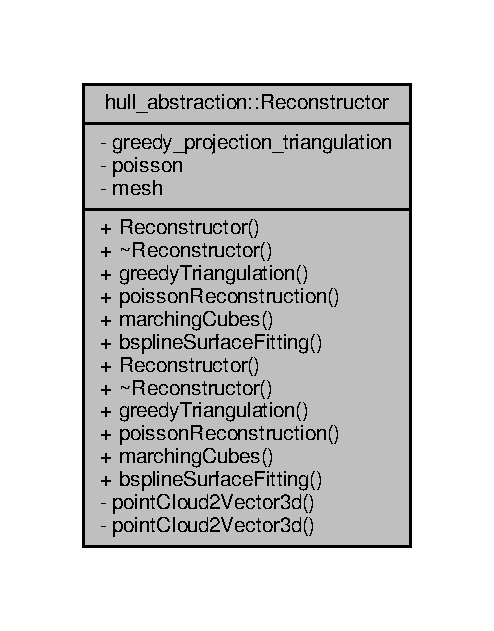
\includegraphics[width=237pt]{classhull__abstraction_1_1_reconstructor__coll__graph}
\end{center}
\end{figure}
\subsection*{Public Member Functions}
\begin{DoxyCompactItemize}
\item 
\hyperlink{classhull__abstraction_1_1_reconstructor_a621404f6ce3a4515adf85491543ace34}{Reconstructor} ()
\begin{DoxyCompactList}\small\item\em Constructor. \end{DoxyCompactList}\item 
\hyperlink{classhull__abstraction_1_1_reconstructor_a0db70f08234b090c7a5c58872dbd16c4}{$\sim$\+Reconstructor} ()
\begin{DoxyCompactList}\small\item\em Deconstructor. \end{DoxyCompactList}\item 
pcl\+::\+Polygon\+Mesh \hyperlink{classhull__abstraction_1_1_reconstructor_a585b9418c1a64ec21c195c72139ce581}{greedy\+Triangulation} (pcl\+::\+Point\+Cloud$<$ pcl\+::\+Point\+Normal $>$\+::Ptr cloud\+\_\+with\+\_\+normals)
\begin{DoxyCompactList}\small\item\em Generate polygon meshes using greedy triangulation algorithm. \end{DoxyCompactList}\item 
pcl\+::\+Polygon\+Mesh \hyperlink{classhull__abstraction_1_1_reconstructor_a9b7e8bda9c001e4d2eab2712e2b57f04}{poisson\+Reconstruction} (pcl\+::\+Point\+Cloud$<$ pcl\+::\+Point\+Normal $>$\+::Ptr cloud\+\_\+with\+\_\+normals)
\begin{DoxyCompactList}\small\item\em Generate polygon meshes through Poisson reconstruction method. \end{DoxyCompactList}\item 
pcl\+::\+Polygon\+Mesh \hyperlink{classhull__abstraction_1_1_reconstructor_a41a0fa653923a21b3329b747f0c6943b}{marching\+Cubes} (pcl\+::\+Point\+Cloud$<$ pcl\+::\+Point\+Normal $>$\+::Ptr cloud\+\_\+with\+\_\+normals)
\begin{DoxyCompactList}\small\item\em Generate polygon meshes utilizing marching cubes method. \end{DoxyCompactList}\item 
pcl\+::\+Polygon\+Mesh \hyperlink{classhull__abstraction_1_1_reconstructor_a531c5dc53b28b4f1e48a318db1acea90}{bspline\+Surface\+Fitting} (pcl\+::\+Point\+Cloud$<$ pcl\+::\+Point\+X\+YZ $>$\+::Ptr cloud)
\begin{DoxyCompactList}\small\item\em Generate polygon meshes based on b-\/spline surface fitting. \end{DoxyCompactList}\item 
\hyperlink{classhull__abstraction_1_1_reconstructor_a621404f6ce3a4515adf85491543ace34}{Reconstructor} ()
\begin{DoxyCompactList}\small\item\em Constructor. \end{DoxyCompactList}\item 
\hyperlink{classhull__abstraction_1_1_reconstructor_a0db70f08234b090c7a5c58872dbd16c4}{$\sim$\+Reconstructor} ()
\begin{DoxyCompactList}\small\item\em Deconstructor. \end{DoxyCompactList}\item 
pcl\+::\+Polygon\+Mesh \hyperlink{classhull__abstraction_1_1_reconstructor_a585b9418c1a64ec21c195c72139ce581}{greedy\+Triangulation} (pcl\+::\+Point\+Cloud$<$ pcl\+::\+Point\+Normal $>$\+::Ptr cloud\+\_\+with\+\_\+normals)
\begin{DoxyCompactList}\small\item\em Generate polygon meshes using greedy triangulation algorithm. \end{DoxyCompactList}\item 
pcl\+::\+Polygon\+Mesh \hyperlink{classhull__abstraction_1_1_reconstructor_a9b7e8bda9c001e4d2eab2712e2b57f04}{poisson\+Reconstruction} (pcl\+::\+Point\+Cloud$<$ pcl\+::\+Point\+Normal $>$\+::Ptr cloud\+\_\+with\+\_\+normals)
\begin{DoxyCompactList}\small\item\em Generate polygon meshes through Poisson reconstruction method. \end{DoxyCompactList}\item 
pcl\+::\+Polygon\+Mesh \hyperlink{classhull__abstraction_1_1_reconstructor_a41a0fa653923a21b3329b747f0c6943b}{marching\+Cubes} (pcl\+::\+Point\+Cloud$<$ pcl\+::\+Point\+Normal $>$\+::Ptr cloud\+\_\+with\+\_\+normals)
\begin{DoxyCompactList}\small\item\em Generate polygon meshes utilizing marching cubes method. \end{DoxyCompactList}\item 
pcl\+::\+Polygon\+Mesh \hyperlink{classhull__abstraction_1_1_reconstructor_a531c5dc53b28b4f1e48a318db1acea90}{bspline\+Surface\+Fitting} (pcl\+::\+Point\+Cloud$<$ pcl\+::\+Point\+X\+YZ $>$\+::Ptr cloud)
\begin{DoxyCompactList}\small\item\em Generate polygon meshes based on b-\/spline surface fitting. \end{DoxyCompactList}\end{DoxyCompactItemize}
\subsection*{Private Member Functions}
\begin{DoxyCompactItemize}
\item 
void \hyperlink{classhull__abstraction_1_1_reconstructor_a484b377810bba7e42d39c47ed3725941}{point\+Cloud2\+Vector3d} (pcl\+::\+Point\+Cloud$<$ pcl\+::\+Point\+X\+YZ $>$\+::Ptr cloud, pcl\+::on\+\_\+nurbs\+::vector\+\_\+vec3d \&data)
\begin{DoxyCompactList}\small\item\em Converting a cloud of Point\+X\+YZ to a set of three-\/dimensional vectors. \end{DoxyCompactList}\item 
void \hyperlink{classhull__abstraction_1_1_reconstructor_a484b377810bba7e42d39c47ed3725941}{point\+Cloud2\+Vector3d} (pcl\+::\+Point\+Cloud$<$ pcl\+::\+Point\+X\+YZ $>$\+::Ptr cloud, pcl\+::on\+\_\+nurbs\+::vector\+\_\+vec3d \&data)
\begin{DoxyCompactList}\small\item\em Converting a cloud of Point\+X\+YZ to a set of three-\/dimensional vectors. \end{DoxyCompactList}\end{DoxyCompactItemize}
\subsection*{Private Attributes}
\begin{DoxyCompactItemize}
\item 
pcl\+::\+Greedy\+Projection\+Triangulation$<$ pcl\+::\+Point\+Normal $>$ \hyperlink{classhull__abstraction_1_1_reconstructor_aeb53b00a5a6300f6fcbef59d6759f01b}{greedy\+\_\+projection\+\_\+triangulation}
\item 
pcl\+::\+Poisson$<$ pcl\+::\+Point\+Normal $>$ \hyperlink{classhull__abstraction_1_1_reconstructor_a60dfa765833af8d05f1426be0e96adb0}{poisson}
\item 
pcl\+::\+Polygon\+Mesh \hyperlink{classhull__abstraction_1_1_reconstructor_af0818936b15dd13f3a9fa3e70734cd57}{mesh}
\end{DoxyCompactItemize}


\subsection{Detailed Description}
The \hyperlink{classhull__abstraction_1_1_reconstructor}{Reconstructor} class. 

This class wraps some hull construction methods for point cloud data 

\subsection{Constructor \& Destructor Documentation}
\index{hull\+\_\+abstraction\+::\+Reconstructor@{hull\+\_\+abstraction\+::\+Reconstructor}!Reconstructor@{Reconstructor}}
\index{Reconstructor@{Reconstructor}!hull\+\_\+abstraction\+::\+Reconstructor@{hull\+\_\+abstraction\+::\+Reconstructor}}
\subsubsection[{\texorpdfstring{Reconstructor()}{Reconstructor()}}]{\setlength{\rightskip}{0pt plus 5cm}hull\+\_\+abstraction\+::\+Reconstructor\+::\+Reconstructor (
\begin{DoxyParamCaption}
{}
\end{DoxyParamCaption}
)\hspace{0.3cm}{\ttfamily [inline]}}\hypertarget{classhull__abstraction_1_1_reconstructor_a621404f6ce3a4515adf85491543ace34}{}\label{classhull__abstraction_1_1_reconstructor_a621404f6ce3a4515adf85491543ace34}


Constructor. 

\index{hull\+\_\+abstraction\+::\+Reconstructor@{hull\+\_\+abstraction\+::\+Reconstructor}!````~Reconstructor@{$\sim$\+Reconstructor}}
\index{````~Reconstructor@{$\sim$\+Reconstructor}!hull\+\_\+abstraction\+::\+Reconstructor@{hull\+\_\+abstraction\+::\+Reconstructor}}
\subsubsection[{\texorpdfstring{$\sim$\+Reconstructor()}{~Reconstructor()}}]{\setlength{\rightskip}{0pt plus 5cm}hull\+\_\+abstraction\+::\+Reconstructor\+::$\sim$\+Reconstructor (
\begin{DoxyParamCaption}
{}
\end{DoxyParamCaption}
)\hspace{0.3cm}{\ttfamily [inline]}}\hypertarget{classhull__abstraction_1_1_reconstructor_a0db70f08234b090c7a5c58872dbd16c4}{}\label{classhull__abstraction_1_1_reconstructor_a0db70f08234b090c7a5c58872dbd16c4}


Deconstructor. 

\index{hull\+\_\+abstraction\+::\+Reconstructor@{hull\+\_\+abstraction\+::\+Reconstructor}!Reconstructor@{Reconstructor}}
\index{Reconstructor@{Reconstructor}!hull\+\_\+abstraction\+::\+Reconstructor@{hull\+\_\+abstraction\+::\+Reconstructor}}
\subsubsection[{\texorpdfstring{Reconstructor()}{Reconstructor()}}]{\setlength{\rightskip}{0pt plus 5cm}hull\+\_\+abstraction\+::\+Reconstructor\+::\+Reconstructor (
\begin{DoxyParamCaption}
{}
\end{DoxyParamCaption}
)\hspace{0.3cm}{\ttfamily [inline]}}\hypertarget{classhull__abstraction_1_1_reconstructor_a621404f6ce3a4515adf85491543ace34}{}\label{classhull__abstraction_1_1_reconstructor_a621404f6ce3a4515adf85491543ace34}


Constructor. 

\index{hull\+\_\+abstraction\+::\+Reconstructor@{hull\+\_\+abstraction\+::\+Reconstructor}!````~Reconstructor@{$\sim$\+Reconstructor}}
\index{````~Reconstructor@{$\sim$\+Reconstructor}!hull\+\_\+abstraction\+::\+Reconstructor@{hull\+\_\+abstraction\+::\+Reconstructor}}
\subsubsection[{\texorpdfstring{$\sim$\+Reconstructor()}{~Reconstructor()}}]{\setlength{\rightskip}{0pt plus 5cm}hull\+\_\+abstraction\+::\+Reconstructor\+::$\sim$\+Reconstructor (
\begin{DoxyParamCaption}
{}
\end{DoxyParamCaption}
)\hspace{0.3cm}{\ttfamily [inline]}}\hypertarget{classhull__abstraction_1_1_reconstructor_a0db70f08234b090c7a5c58872dbd16c4}{}\label{classhull__abstraction_1_1_reconstructor_a0db70f08234b090c7a5c58872dbd16c4}


Deconstructor. 



\subsection{Member Function Documentation}
\index{hull\+\_\+abstraction\+::\+Reconstructor@{hull\+\_\+abstraction\+::\+Reconstructor}!bspline\+Surface\+Fitting@{bspline\+Surface\+Fitting}}
\index{bspline\+Surface\+Fitting@{bspline\+Surface\+Fitting}!hull\+\_\+abstraction\+::\+Reconstructor@{hull\+\_\+abstraction\+::\+Reconstructor}}
\subsubsection[{\texorpdfstring{bspline\+Surface\+Fitting(pcl\+::\+Point\+Cloud$<$ pcl\+::\+Point\+X\+Y\+Z $>$\+::\+Ptr cloud)}{bsplineSurfaceFitting(pcl::PointCloud< pcl::PointXYZ >::Ptr cloud)}}]{\setlength{\rightskip}{0pt plus 5cm}pcl\+::\+Polygon\+Mesh hull\+\_\+abstraction\+::\+Reconstructor\+::bspline\+Surface\+Fitting (
\begin{DoxyParamCaption}
\item[{pcl\+::\+Point\+Cloud$<$ pcl\+::\+Point\+X\+YZ $>$\+::Ptr}]{cloud}
\end{DoxyParamCaption}
)}\hypertarget{classhull__abstraction_1_1_reconstructor_a531c5dc53b28b4f1e48a318db1acea90}{}\label{classhull__abstraction_1_1_reconstructor_a531c5dc53b28b4f1e48a318db1acea90}


Generate polygon meshes based on b-\/spline surface fitting. 


\begin{DoxyParams}{Parameters}
{\em cloud} & Cloud of Point\+X\+YZ \\
\hline
\end{DoxyParams}
\begin{DoxyReturn}{Returns}
Resulting polygon meshes of cloud\+\_\+with\+\_\+normals 
\end{DoxyReturn}
$<$ Data structure for N\+U\+R\+BS surface fitting \index{hull\+\_\+abstraction\+::\+Reconstructor@{hull\+\_\+abstraction\+::\+Reconstructor}!bspline\+Surface\+Fitting@{bspline\+Surface\+Fitting}}
\index{bspline\+Surface\+Fitting@{bspline\+Surface\+Fitting}!hull\+\_\+abstraction\+::\+Reconstructor@{hull\+\_\+abstraction\+::\+Reconstructor}}
\subsubsection[{\texorpdfstring{bspline\+Surface\+Fitting(pcl\+::\+Point\+Cloud$<$ pcl\+::\+Point\+X\+Y\+Z $>$\+::\+Ptr cloud)}{bsplineSurfaceFitting(pcl::PointCloud< pcl::PointXYZ >::Ptr cloud)}}]{\setlength{\rightskip}{0pt plus 5cm}pcl\+::\+Polygon\+Mesh hull\+\_\+abstraction\+::\+Reconstructor\+::bspline\+Surface\+Fitting (
\begin{DoxyParamCaption}
\item[{pcl\+::\+Point\+Cloud$<$ pcl\+::\+Point\+X\+YZ $>$\+::Ptr}]{cloud}
\end{DoxyParamCaption}
)}\hypertarget{classhull__abstraction_1_1_reconstructor_a531c5dc53b28b4f1e48a318db1acea90}{}\label{classhull__abstraction_1_1_reconstructor_a531c5dc53b28b4f1e48a318db1acea90}


Generate polygon meshes based on b-\/spline surface fitting. 


\begin{DoxyParams}{Parameters}
{\em cloud} & Cloud of Point\+X\+YZ \\
\hline
\end{DoxyParams}
\begin{DoxyReturn}{Returns}
Resulting polygon meshes of cloud\+\_\+with\+\_\+normals 
\end{DoxyReturn}
\index{hull\+\_\+abstraction\+::\+Reconstructor@{hull\+\_\+abstraction\+::\+Reconstructor}!greedy\+Triangulation@{greedy\+Triangulation}}
\index{greedy\+Triangulation@{greedy\+Triangulation}!hull\+\_\+abstraction\+::\+Reconstructor@{hull\+\_\+abstraction\+::\+Reconstructor}}
\subsubsection[{\texorpdfstring{greedy\+Triangulation(pcl\+::\+Point\+Cloud$<$ pcl\+::\+Point\+Normal $>$\+::\+Ptr cloud\+\_\+with\+\_\+normals)}{greedyTriangulation(pcl::PointCloud< pcl::PointNormal >::Ptr cloud_with_normals)}}]{\setlength{\rightskip}{0pt plus 5cm}pcl\+::\+Polygon\+Mesh hull\+\_\+abstraction\+::\+Reconstructor\+::greedy\+Triangulation (
\begin{DoxyParamCaption}
\item[{pcl\+::\+Point\+Cloud$<$ pcl\+::\+Point\+Normal $>$\+::Ptr}]{cloud\+\_\+with\+\_\+normals}
\end{DoxyParamCaption}
)}\hypertarget{classhull__abstraction_1_1_reconstructor_a585b9418c1a64ec21c195c72139ce581}{}\label{classhull__abstraction_1_1_reconstructor_a585b9418c1a64ec21c195c72139ce581}


Generate polygon meshes using greedy triangulation algorithm. 


\begin{DoxyParams}{Parameters}
{\em cloud\+\_\+with\+\_\+normals} & Cloud of Point\+Normal \\
\hline
\end{DoxyParams}
\begin{DoxyReturn}{Returns}
Resulting polygon meshes of cloud\+\_\+with\+\_\+normals 
\end{DoxyReturn}
\index{hull\+\_\+abstraction\+::\+Reconstructor@{hull\+\_\+abstraction\+::\+Reconstructor}!greedy\+Triangulation@{greedy\+Triangulation}}
\index{greedy\+Triangulation@{greedy\+Triangulation}!hull\+\_\+abstraction\+::\+Reconstructor@{hull\+\_\+abstraction\+::\+Reconstructor}}
\subsubsection[{\texorpdfstring{greedy\+Triangulation(pcl\+::\+Point\+Cloud$<$ pcl\+::\+Point\+Normal $>$\+::\+Ptr cloud\+\_\+with\+\_\+normals)}{greedyTriangulation(pcl::PointCloud< pcl::PointNormal >::Ptr cloud_with_normals)}}]{\setlength{\rightskip}{0pt plus 5cm}pcl\+::\+Polygon\+Mesh hull\+\_\+abstraction\+::\+Reconstructor\+::greedy\+Triangulation (
\begin{DoxyParamCaption}
\item[{pcl\+::\+Point\+Cloud$<$ pcl\+::\+Point\+Normal $>$\+::Ptr}]{cloud\+\_\+with\+\_\+normals}
\end{DoxyParamCaption}
)}\hypertarget{classhull__abstraction_1_1_reconstructor_a585b9418c1a64ec21c195c72139ce581}{}\label{classhull__abstraction_1_1_reconstructor_a585b9418c1a64ec21c195c72139ce581}


Generate polygon meshes using greedy triangulation algorithm. 


\begin{DoxyParams}{Parameters}
{\em cloud\+\_\+with\+\_\+normals} & Cloud of Point\+Normal \\
\hline
\end{DoxyParams}
\begin{DoxyReturn}{Returns}
Resulting polygon meshes of cloud\+\_\+with\+\_\+normals 
\end{DoxyReturn}
\index{hull\+\_\+abstraction\+::\+Reconstructor@{hull\+\_\+abstraction\+::\+Reconstructor}!marching\+Cubes@{marching\+Cubes}}
\index{marching\+Cubes@{marching\+Cubes}!hull\+\_\+abstraction\+::\+Reconstructor@{hull\+\_\+abstraction\+::\+Reconstructor}}
\subsubsection[{\texorpdfstring{marching\+Cubes(pcl\+::\+Point\+Cloud$<$ pcl\+::\+Point\+Normal $>$\+::\+Ptr cloud\+\_\+with\+\_\+normals)}{marchingCubes(pcl::PointCloud< pcl::PointNormal >::Ptr cloud_with_normals)}}]{\setlength{\rightskip}{0pt plus 5cm}pcl\+::\+Polygon\+Mesh hull\+\_\+abstraction\+::\+Reconstructor\+::marching\+Cubes (
\begin{DoxyParamCaption}
\item[{pcl\+::\+Point\+Cloud$<$ pcl\+::\+Point\+Normal $>$\+::Ptr}]{cloud\+\_\+with\+\_\+normals}
\end{DoxyParamCaption}
)}\hypertarget{classhull__abstraction_1_1_reconstructor_a41a0fa653923a21b3329b747f0c6943b}{}\label{classhull__abstraction_1_1_reconstructor_a41a0fa653923a21b3329b747f0c6943b}


Generate polygon meshes utilizing marching cubes method. 


\begin{DoxyParams}{Parameters}
{\em cloud\+\_\+with\+\_\+normals} & Cloud of Point\+Normal \\
\hline
\end{DoxyParams}
\begin{DoxyReturn}{Returns}
Resulting polygon meshes of cloud\+\_\+with\+\_\+normals 
\end{DoxyReturn}
\index{hull\+\_\+abstraction\+::\+Reconstructor@{hull\+\_\+abstraction\+::\+Reconstructor}!marching\+Cubes@{marching\+Cubes}}
\index{marching\+Cubes@{marching\+Cubes}!hull\+\_\+abstraction\+::\+Reconstructor@{hull\+\_\+abstraction\+::\+Reconstructor}}
\subsubsection[{\texorpdfstring{marching\+Cubes(pcl\+::\+Point\+Cloud$<$ pcl\+::\+Point\+Normal $>$\+::\+Ptr cloud\+\_\+with\+\_\+normals)}{marchingCubes(pcl::PointCloud< pcl::PointNormal >::Ptr cloud_with_normals)}}]{\setlength{\rightskip}{0pt plus 5cm}pcl\+::\+Polygon\+Mesh hull\+\_\+abstraction\+::\+Reconstructor\+::marching\+Cubes (
\begin{DoxyParamCaption}
\item[{pcl\+::\+Point\+Cloud$<$ pcl\+::\+Point\+Normal $>$\+::Ptr}]{cloud\+\_\+with\+\_\+normals}
\end{DoxyParamCaption}
)}\hypertarget{classhull__abstraction_1_1_reconstructor_a41a0fa653923a21b3329b747f0c6943b}{}\label{classhull__abstraction_1_1_reconstructor_a41a0fa653923a21b3329b747f0c6943b}


Generate polygon meshes utilizing marching cubes method. 


\begin{DoxyParams}{Parameters}
{\em cloud\+\_\+with\+\_\+normals} & Cloud of Point\+Normal \\
\hline
\end{DoxyParams}
\begin{DoxyReturn}{Returns}
Resulting polygon meshes of cloud\+\_\+with\+\_\+normals 
\end{DoxyReturn}
\index{hull\+\_\+abstraction\+::\+Reconstructor@{hull\+\_\+abstraction\+::\+Reconstructor}!point\+Cloud2\+Vector3d@{point\+Cloud2\+Vector3d}}
\index{point\+Cloud2\+Vector3d@{point\+Cloud2\+Vector3d}!hull\+\_\+abstraction\+::\+Reconstructor@{hull\+\_\+abstraction\+::\+Reconstructor}}
\subsubsection[{\texorpdfstring{point\+Cloud2\+Vector3d(pcl\+::\+Point\+Cloud$<$ pcl\+::\+Point\+X\+Y\+Z $>$\+::\+Ptr cloud, pcl\+::on\+\_\+nurbs\+::vector\+\_\+vec3d \&data)}{pointCloud2Vector3d(pcl::PointCloud< pcl::PointXYZ >::Ptr cloud, pcl::on_nurbs::vector_vec3d &data)}}]{\setlength{\rightskip}{0pt plus 5cm}void hull\+\_\+abstraction\+::\+Reconstructor\+::point\+Cloud2\+Vector3d (
\begin{DoxyParamCaption}
\item[{pcl\+::\+Point\+Cloud$<$ pcl\+::\+Point\+X\+YZ $>$\+::Ptr}]{cloud, }
\item[{pcl\+::on\+\_\+nurbs\+::vector\+\_\+vec3d \&}]{data}
\end{DoxyParamCaption}
)\hspace{0.3cm}{\ttfamily [private]}}\hypertarget{classhull__abstraction_1_1_reconstructor_a484b377810bba7e42d39c47ed3725941}{}\label{classhull__abstraction_1_1_reconstructor_a484b377810bba7e42d39c47ed3725941}


Converting a cloud of Point\+X\+YZ to a set of three-\/dimensional vectors. 


\begin{DoxyParams}[1]{Parameters}
\mbox{\tt in}  & {\em cloud} & Cloud of Point\+X\+YZ \\
\hline
\mbox{\tt out}  & {\em data} & A set of three-\/dimentional vectors \\
\hline
\end{DoxyParams}
\index{hull\+\_\+abstraction\+::\+Reconstructor@{hull\+\_\+abstraction\+::\+Reconstructor}!point\+Cloud2\+Vector3d@{point\+Cloud2\+Vector3d}}
\index{point\+Cloud2\+Vector3d@{point\+Cloud2\+Vector3d}!hull\+\_\+abstraction\+::\+Reconstructor@{hull\+\_\+abstraction\+::\+Reconstructor}}
\subsubsection[{\texorpdfstring{point\+Cloud2\+Vector3d(pcl\+::\+Point\+Cloud$<$ pcl\+::\+Point\+X\+Y\+Z $>$\+::\+Ptr cloud, pcl\+::on\+\_\+nurbs\+::vector\+\_\+vec3d \&data)}{pointCloud2Vector3d(pcl::PointCloud< pcl::PointXYZ >::Ptr cloud, pcl::on_nurbs::vector_vec3d &data)}}]{\setlength{\rightskip}{0pt plus 5cm}void hull\+\_\+abstraction\+::\+Reconstructor\+::point\+Cloud2\+Vector3d (
\begin{DoxyParamCaption}
\item[{pcl\+::\+Point\+Cloud$<$ pcl\+::\+Point\+X\+YZ $>$\+::Ptr}]{cloud, }
\item[{pcl\+::on\+\_\+nurbs\+::vector\+\_\+vec3d \&}]{data}
\end{DoxyParamCaption}
)\hspace{0.3cm}{\ttfamily [private]}}\hypertarget{classhull__abstraction_1_1_reconstructor_a484b377810bba7e42d39c47ed3725941}{}\label{classhull__abstraction_1_1_reconstructor_a484b377810bba7e42d39c47ed3725941}


Converting a cloud of Point\+X\+YZ to a set of three-\/dimensional vectors. 


\begin{DoxyParams}[1]{Parameters}
\mbox{\tt in}  & {\em cloud} & Cloud of Point\+X\+YZ \\
\hline
\mbox{\tt out}  & {\em data} & A set of three-\/dimentional vectors \\
\hline
\end{DoxyParams}
\index{hull\+\_\+abstraction\+::\+Reconstructor@{hull\+\_\+abstraction\+::\+Reconstructor}!poisson\+Reconstruction@{poisson\+Reconstruction}}
\index{poisson\+Reconstruction@{poisson\+Reconstruction}!hull\+\_\+abstraction\+::\+Reconstructor@{hull\+\_\+abstraction\+::\+Reconstructor}}
\subsubsection[{\texorpdfstring{poisson\+Reconstruction(pcl\+::\+Point\+Cloud$<$ pcl\+::\+Point\+Normal $>$\+::\+Ptr cloud\+\_\+with\+\_\+normals)}{poissonReconstruction(pcl::PointCloud< pcl::PointNormal >::Ptr cloud_with_normals)}}]{\setlength{\rightskip}{0pt plus 5cm}pcl\+::\+Polygon\+Mesh hull\+\_\+abstraction\+::\+Reconstructor\+::poisson\+Reconstruction (
\begin{DoxyParamCaption}
\item[{pcl\+::\+Point\+Cloud$<$ pcl\+::\+Point\+Normal $>$\+::Ptr}]{cloud\+\_\+with\+\_\+normals}
\end{DoxyParamCaption}
)}\hypertarget{classhull__abstraction_1_1_reconstructor_a9b7e8bda9c001e4d2eab2712e2b57f04}{}\label{classhull__abstraction_1_1_reconstructor_a9b7e8bda9c001e4d2eab2712e2b57f04}


Generate polygon meshes through Poisson reconstruction method. 


\begin{DoxyParams}{Parameters}
{\em cloud\+\_\+with\+\_\+normals} & Cloud of Point\+Normal \\
\hline
\end{DoxyParams}
\begin{DoxyReturn}{Returns}
Resulting polygon meshes of cloud\+\_\+with\+\_\+normals 
\end{DoxyReturn}
\index{hull\+\_\+abstraction\+::\+Reconstructor@{hull\+\_\+abstraction\+::\+Reconstructor}!poisson\+Reconstruction@{poisson\+Reconstruction}}
\index{poisson\+Reconstruction@{poisson\+Reconstruction}!hull\+\_\+abstraction\+::\+Reconstructor@{hull\+\_\+abstraction\+::\+Reconstructor}}
\subsubsection[{\texorpdfstring{poisson\+Reconstruction(pcl\+::\+Point\+Cloud$<$ pcl\+::\+Point\+Normal $>$\+::\+Ptr cloud\+\_\+with\+\_\+normals)}{poissonReconstruction(pcl::PointCloud< pcl::PointNormal >::Ptr cloud_with_normals)}}]{\setlength{\rightskip}{0pt plus 5cm}pcl\+::\+Polygon\+Mesh hull\+\_\+abstraction\+::\+Reconstructor\+::poisson\+Reconstruction (
\begin{DoxyParamCaption}
\item[{pcl\+::\+Point\+Cloud$<$ pcl\+::\+Point\+Normal $>$\+::Ptr}]{cloud\+\_\+with\+\_\+normals}
\end{DoxyParamCaption}
)}\hypertarget{classhull__abstraction_1_1_reconstructor_a9b7e8bda9c001e4d2eab2712e2b57f04}{}\label{classhull__abstraction_1_1_reconstructor_a9b7e8bda9c001e4d2eab2712e2b57f04}


Generate polygon meshes through Poisson reconstruction method. 


\begin{DoxyParams}{Parameters}
{\em cloud\+\_\+with\+\_\+normals} & Cloud of Point\+Normal \\
\hline
\end{DoxyParams}
\begin{DoxyReturn}{Returns}
Resulting polygon meshes of cloud\+\_\+with\+\_\+normals 
\end{DoxyReturn}


\subsection{Member Data Documentation}
\index{hull\+\_\+abstraction\+::\+Reconstructor@{hull\+\_\+abstraction\+::\+Reconstructor}!greedy\+\_\+projection\+\_\+triangulation@{greedy\+\_\+projection\+\_\+triangulation}}
\index{greedy\+\_\+projection\+\_\+triangulation@{greedy\+\_\+projection\+\_\+triangulation}!hull\+\_\+abstraction\+::\+Reconstructor@{hull\+\_\+abstraction\+::\+Reconstructor}}
\subsubsection[{\texorpdfstring{greedy\+\_\+projection\+\_\+triangulation}{greedy_projection_triangulation}}]{\setlength{\rightskip}{0pt plus 5cm}pcl\+::\+Greedy\+Projection\+Triangulation$<$ pcl\+::\+Point\+Normal $>$ hull\+\_\+abstraction\+::\+Reconstructor\+::greedy\+\_\+projection\+\_\+triangulation\hspace{0.3cm}{\ttfamily [private]}}\hypertarget{classhull__abstraction_1_1_reconstructor_aeb53b00a5a6300f6fcbef59d6759f01b}{}\label{classhull__abstraction_1_1_reconstructor_aeb53b00a5a6300f6fcbef59d6759f01b}
Object for performing greedy triangulation algorithm \index{hull\+\_\+abstraction\+::\+Reconstructor@{hull\+\_\+abstraction\+::\+Reconstructor}!mesh@{mesh}}
\index{mesh@{mesh}!hull\+\_\+abstraction\+::\+Reconstructor@{hull\+\_\+abstraction\+::\+Reconstructor}}
\subsubsection[{\texorpdfstring{mesh}{mesh}}]{\setlength{\rightskip}{0pt plus 5cm}pcl\+::\+Polygon\+Mesh hull\+\_\+abstraction\+::\+Reconstructor\+::mesh\hspace{0.3cm}{\ttfamily [private]}}\hypertarget{classhull__abstraction_1_1_reconstructor_af0818936b15dd13f3a9fa3e70734cd57}{}\label{classhull__abstraction_1_1_reconstructor_af0818936b15dd13f3a9fa3e70734cd57}
Result of polygon meshes generation \index{hull\+\_\+abstraction\+::\+Reconstructor@{hull\+\_\+abstraction\+::\+Reconstructor}!poisson@{poisson}}
\index{poisson@{poisson}!hull\+\_\+abstraction\+::\+Reconstructor@{hull\+\_\+abstraction\+::\+Reconstructor}}
\subsubsection[{\texorpdfstring{poisson}{poisson}}]{\setlength{\rightskip}{0pt plus 5cm}pcl\+::\+Poisson$<$ pcl\+::\+Point\+Normal $>$ hull\+\_\+abstraction\+::\+Reconstructor\+::poisson\hspace{0.3cm}{\ttfamily [private]}}\hypertarget{classhull__abstraction_1_1_reconstructor_a60dfa765833af8d05f1426be0e96adb0}{}\label{classhull__abstraction_1_1_reconstructor_a60dfa765833af8d05f1426be0e96adb0}
Object for performing Poisson reconstruction 

The documentation for this class was generated from the following files\+:\begin{DoxyCompactItemize}
\item 
/home/jc/\+T\+H\+E\+S\+I\+S/hull\+\_\+abstraction/benchmark/include/hull\+\_\+abstraction/\hyperlink{benchmark_2include_2hull__abstraction_2reconstructor_8h}{reconstructor.\+h}\item 
/home/jc/\+T\+H\+E\+S\+I\+S/hull\+\_\+abstraction/benchmark/src/hull\+\_\+abstraction/\hyperlink{benchmark_2src_2hull__abstraction_2reconstructor_8cpp}{reconstructor.\+cpp}\end{DoxyCompactItemize}

\chapter{File Documentation}
\hypertarget{_n_o_t_e_s_8md}{}\section{/home/jc/hull\+\_\+abstraction/\+N\+O\+T\+ES.md File Reference}
\label{_n_o_t_e_s_8md}\index{/home/jc/hull\+\_\+abstraction/\+N\+O\+T\+E\+S.\+md@{/home/jc/hull\+\_\+abstraction/\+N\+O\+T\+E\+S.\+md}}

\hypertarget{prototype_2build_2_c_make_files_23_85_81_2_compiler_id_c_2_c_make_c_compiler_id_8c}{}\section{/home/jc/hull\+\_\+abstraction/prototype/build/\+C\+Make\+Files/3.5.1/\+Compiler\+Id\+C/\+C\+Make\+C\+Compiler\+Id.c File Reference}
\label{prototype_2build_2_c_make_files_23_85_81_2_compiler_id_c_2_c_make_c_compiler_id_8c}\index{/home/jc/hull\+\_\+abstraction/prototype/build/\+C\+Make\+Files/3.\+5.\+1/\+Compiler\+Id\+C/\+C\+Make\+C\+Compiler\+Id.\+c@{/home/jc/hull\+\_\+abstraction/prototype/build/\+C\+Make\+Files/3.\+5.\+1/\+Compiler\+Id\+C/\+C\+Make\+C\+Compiler\+Id.\+c}}
\subsection*{Macros}
\begin{DoxyCompactItemize}
\item 
\#define \hyperlink{prototype_2build_2_c_make_files_23_85_81_2_compiler_id_c_2_c_make_c_compiler_id_8c_a81dee0709ded976b2e0319239f72d174}{C\+O\+M\+P\+I\+L\+E\+R\+\_\+\+ID}~\char`\"{}\char`\"{}
\item 
\#define \hyperlink{prototype_2build_2_c_make_files_23_85_81_2_compiler_id_c_2_c_make_c_compiler_id_8c_a2ae9b72bb13abaabfcf2ee0ba7d3fa1d}{S\+T\+R\+I\+N\+G\+I\+F\+Y\+\_\+\+H\+E\+L\+P\+ER}(X)~\#X
\item 
\#define \hyperlink{prototype_2build_2_c_make_files_23_85_81_2_compiler_id_c_2_c_make_c_compiler_id_8c_a43e1cad902b6477bec893cb6430bd6c8}{S\+T\+R\+I\+N\+G\+I\+FY}(X)~\hyperlink{ros_2build_2_c_make_files_23_85_81_2_compiler_id_c_x_x_2_c_make_c_x_x_compiler_id_8cpp_a2ae9b72bb13abaabfcf2ee0ba7d3fa1d}{S\+T\+R\+I\+N\+G\+I\+F\+Y\+\_\+\+H\+E\+L\+P\+ER}(X)
\item 
\#define \hyperlink{prototype_2build_2_c_make_files_23_85_81_2_compiler_id_c_2_c_make_c_compiler_id_8c_adbc5372f40838899018fadbc89bd588b}{P\+L\+A\+T\+F\+O\+R\+M\+\_\+\+ID}~\char`\"{}\char`\"{}
\item 
\#define \hyperlink{prototype_2build_2_c_make_files_23_85_81_2_compiler_id_c_2_c_make_c_compiler_id_8c_aba35d0d200deaeb06aee95ca297acb28}{A\+R\+C\+H\+I\+T\+E\+C\+T\+U\+R\+E\+\_\+\+ID}~\char`\"{}\char`\"{}
\item 
\#define \hyperlink{prototype_2build_2_c_make_files_23_85_81_2_compiler_id_c_2_c_make_c_compiler_id_8c_ad1280362da42492bbc11aa78cbf776ad}{D\+EC}(n)
\item 
\#define \hyperlink{prototype_2build_2_c_make_files_23_85_81_2_compiler_id_c_2_c_make_c_compiler_id_8c_a46d5d95daa1bef867bd0179594310ed5}{H\+EX}(n)
\end{DoxyCompactItemize}
\subsection*{Functions}
\begin{DoxyCompactItemize}
\item 
int \hyperlink{prototype_2build_2_c_make_files_23_85_81_2_compiler_id_c_2_c_make_c_compiler_id_8c_a0ddf1224851353fc92bfbff6f499fa97}{main} (int argc, char $\ast$argv\mbox{[}$\,$\mbox{]})
\end{DoxyCompactItemize}
\subsection*{Variables}
\begin{DoxyCompactItemize}
\item 
char const $\ast$ \hyperlink{prototype_2build_2_c_make_files_23_85_81_2_compiler_id_c_2_c_make_c_compiler_id_8c_a4b0efeb7a5d59313986b3a0390f050f6}{info\+\_\+compiler} = \char`\"{}I\+N\+FO\char`\"{} \char`\"{}\+:\char`\"{} \char`\"{}compiler\mbox{[}\char`\"{} C\+O\+M\+P\+I\+L\+E\+R\+\_\+\+ID \char`\"{}\mbox{]}\char`\"{}
\item 
char const $\ast$ \hyperlink{prototype_2build_2_c_make_files_23_85_81_2_compiler_id_c_2_c_make_c_compiler_id_8c_a2321403dee54ee23f0c2fa849c60f7d4}{info\+\_\+platform} = \char`\"{}I\+N\+FO\char`\"{} \char`\"{}\+:\char`\"{} \char`\"{}platform\mbox{[}\char`\"{} P\+L\+A\+T\+F\+O\+R\+M\+\_\+\+ID \char`\"{}\mbox{]}\char`\"{}
\item 
char const $\ast$ \hyperlink{prototype_2build_2_c_make_files_23_85_81_2_compiler_id_c_2_c_make_c_compiler_id_8c_a59647e99d304ed33b15cb284c27ed391}{info\+\_\+arch} = \char`\"{}I\+N\+FO\char`\"{} \char`\"{}\+:\char`\"{} \char`\"{}arch\mbox{[}\char`\"{} A\+R\+C\+H\+I\+T\+E\+C\+T\+U\+R\+E\+\_\+\+ID \char`\"{}\mbox{]}\char`\"{}
\item 
const char $\ast$ \hyperlink{prototype_2build_2_c_make_files_23_85_81_2_compiler_id_c_2_c_make_c_compiler_id_8c_a1ce162bad2fe6966ac8b33cc19e120b8}{info\+\_\+language\+\_\+dialect\+\_\+default}
\end{DoxyCompactItemize}


\subsection{Macro Definition Documentation}
\index{prototype/build/\+C\+Make\+Files/3.\+5.\+1/\+Compiler\+Id\+C/\+C\+Make\+C\+Compiler\+Id.\+c@{prototype/build/\+C\+Make\+Files/3.\+5.\+1/\+Compiler\+Id\+C/\+C\+Make\+C\+Compiler\+Id.\+c}!A\+R\+C\+H\+I\+T\+E\+C\+T\+U\+R\+E\+\_\+\+ID@{A\+R\+C\+H\+I\+T\+E\+C\+T\+U\+R\+E\+\_\+\+ID}}
\index{A\+R\+C\+H\+I\+T\+E\+C\+T\+U\+R\+E\+\_\+\+ID@{A\+R\+C\+H\+I\+T\+E\+C\+T\+U\+R\+E\+\_\+\+ID}!prototype/build/\+C\+Make\+Files/3.\+5.\+1/\+Compiler\+Id\+C/\+C\+Make\+C\+Compiler\+Id.\+c@{prototype/build/\+C\+Make\+Files/3.\+5.\+1/\+Compiler\+Id\+C/\+C\+Make\+C\+Compiler\+Id.\+c}}
\subsubsection[{\texorpdfstring{A\+R\+C\+H\+I\+T\+E\+C\+T\+U\+R\+E\+\_\+\+ID}{ARCHITECTURE_ID}}]{\setlength{\rightskip}{0pt plus 5cm}\#define A\+R\+C\+H\+I\+T\+E\+C\+T\+U\+R\+E\+\_\+\+ID~\char`\"{}\char`\"{}}\hypertarget{prototype_2build_2_c_make_files_23_85_81_2_compiler_id_c_2_c_make_c_compiler_id_8c_aba35d0d200deaeb06aee95ca297acb28}{}\label{prototype_2build_2_c_make_files_23_85_81_2_compiler_id_c_2_c_make_c_compiler_id_8c_aba35d0d200deaeb06aee95ca297acb28}
\index{prototype/build/\+C\+Make\+Files/3.\+5.\+1/\+Compiler\+Id\+C/\+C\+Make\+C\+Compiler\+Id.\+c@{prototype/build/\+C\+Make\+Files/3.\+5.\+1/\+Compiler\+Id\+C/\+C\+Make\+C\+Compiler\+Id.\+c}!C\+O\+M\+P\+I\+L\+E\+R\+\_\+\+ID@{C\+O\+M\+P\+I\+L\+E\+R\+\_\+\+ID}}
\index{C\+O\+M\+P\+I\+L\+E\+R\+\_\+\+ID@{C\+O\+M\+P\+I\+L\+E\+R\+\_\+\+ID}!prototype/build/\+C\+Make\+Files/3.\+5.\+1/\+Compiler\+Id\+C/\+C\+Make\+C\+Compiler\+Id.\+c@{prototype/build/\+C\+Make\+Files/3.\+5.\+1/\+Compiler\+Id\+C/\+C\+Make\+C\+Compiler\+Id.\+c}}
\subsubsection[{\texorpdfstring{C\+O\+M\+P\+I\+L\+E\+R\+\_\+\+ID}{COMPILER_ID}}]{\setlength{\rightskip}{0pt plus 5cm}\#define C\+O\+M\+P\+I\+L\+E\+R\+\_\+\+ID~\char`\"{}\char`\"{}}\hypertarget{prototype_2build_2_c_make_files_23_85_81_2_compiler_id_c_2_c_make_c_compiler_id_8c_a81dee0709ded976b2e0319239f72d174}{}\label{prototype_2build_2_c_make_files_23_85_81_2_compiler_id_c_2_c_make_c_compiler_id_8c_a81dee0709ded976b2e0319239f72d174}
\index{prototype/build/\+C\+Make\+Files/3.\+5.\+1/\+Compiler\+Id\+C/\+C\+Make\+C\+Compiler\+Id.\+c@{prototype/build/\+C\+Make\+Files/3.\+5.\+1/\+Compiler\+Id\+C/\+C\+Make\+C\+Compiler\+Id.\+c}!D\+EC@{D\+EC}}
\index{D\+EC@{D\+EC}!prototype/build/\+C\+Make\+Files/3.\+5.\+1/\+Compiler\+Id\+C/\+C\+Make\+C\+Compiler\+Id.\+c@{prototype/build/\+C\+Make\+Files/3.\+5.\+1/\+Compiler\+Id\+C/\+C\+Make\+C\+Compiler\+Id.\+c}}
\subsubsection[{\texorpdfstring{D\+EC}{DEC}}]{\setlength{\rightskip}{0pt plus 5cm}\#define D\+EC(
\begin{DoxyParamCaption}
\item[{}]{n}
\end{DoxyParamCaption}
)}\hypertarget{prototype_2build_2_c_make_files_23_85_81_2_compiler_id_c_2_c_make_c_compiler_id_8c_ad1280362da42492bbc11aa78cbf776ad}{}\label{prototype_2build_2_c_make_files_23_85_81_2_compiler_id_c_2_c_make_c_compiler_id_8c_ad1280362da42492bbc11aa78cbf776ad}
{\bfseries Value\+:}
\begin{DoxyCode}
(\textcolor{charliteral}{'0'} + (((n) / 10000000)%10)), \(\backslash\)
  (\textcolor{charliteral}{'0'} + (((n) / 1000000)%10)),  \(\backslash\)
  (\textcolor{charliteral}{'0'} + (((n) / 100000)%10)),   \(\backslash\)
  (\textcolor{charliteral}{'0'} + (((n) / 10000)%10)),    \(\backslash\)
  (\textcolor{charliteral}{'0'} + (((n) / 1000)%10)),     \(\backslash\)
  (\textcolor{charliteral}{'0'} + (((n) / 100)%10)),      \(\backslash\)
  (\textcolor{charliteral}{'0'} + (((n) / 10)%10)),       \(\backslash\)
  (\textcolor{charliteral}{'0'} +  ((n) % 10))
\end{DoxyCode}
\index{prototype/build/\+C\+Make\+Files/3.\+5.\+1/\+Compiler\+Id\+C/\+C\+Make\+C\+Compiler\+Id.\+c@{prototype/build/\+C\+Make\+Files/3.\+5.\+1/\+Compiler\+Id\+C/\+C\+Make\+C\+Compiler\+Id.\+c}!H\+EX@{H\+EX}}
\index{H\+EX@{H\+EX}!prototype/build/\+C\+Make\+Files/3.\+5.\+1/\+Compiler\+Id\+C/\+C\+Make\+C\+Compiler\+Id.\+c@{prototype/build/\+C\+Make\+Files/3.\+5.\+1/\+Compiler\+Id\+C/\+C\+Make\+C\+Compiler\+Id.\+c}}
\subsubsection[{\texorpdfstring{H\+EX}{HEX}}]{\setlength{\rightskip}{0pt plus 5cm}\#define H\+EX(
\begin{DoxyParamCaption}
\item[{}]{n}
\end{DoxyParamCaption}
)}\hypertarget{prototype_2build_2_c_make_files_23_85_81_2_compiler_id_c_2_c_make_c_compiler_id_8c_a46d5d95daa1bef867bd0179594310ed5}{}\label{prototype_2build_2_c_make_files_23_85_81_2_compiler_id_c_2_c_make_c_compiler_id_8c_a46d5d95daa1bef867bd0179594310ed5}
{\bfseries Value\+:}
\begin{DoxyCode}
(\textcolor{charliteral}{'0'} + ((n)>>28 & 0xF)), \(\backslash\)
  (\textcolor{charliteral}{'0'} + ((n)>>24 & 0xF)), \(\backslash\)
  (\textcolor{charliteral}{'0'} + ((n)>>20 & 0xF)), \(\backslash\)
  (\textcolor{charliteral}{'0'} + ((n)>>16 & 0xF)), \(\backslash\)
  (\textcolor{charliteral}{'0'} + ((n)>>12 & 0xF)), \(\backslash\)
  (\textcolor{charliteral}{'0'} + ((n)>>8  & 0xF)), \(\backslash\)
  (\textcolor{charliteral}{'0'} + ((n)>>4  & 0xF)), \(\backslash\)
  (\textcolor{charliteral}{'0'} + ((n)     & 0xF))
\end{DoxyCode}
\index{prototype/build/\+C\+Make\+Files/3.\+5.\+1/\+Compiler\+Id\+C/\+C\+Make\+C\+Compiler\+Id.\+c@{prototype/build/\+C\+Make\+Files/3.\+5.\+1/\+Compiler\+Id\+C/\+C\+Make\+C\+Compiler\+Id.\+c}!P\+L\+A\+T\+F\+O\+R\+M\+\_\+\+ID@{P\+L\+A\+T\+F\+O\+R\+M\+\_\+\+ID}}
\index{P\+L\+A\+T\+F\+O\+R\+M\+\_\+\+ID@{P\+L\+A\+T\+F\+O\+R\+M\+\_\+\+ID}!prototype/build/\+C\+Make\+Files/3.\+5.\+1/\+Compiler\+Id\+C/\+C\+Make\+C\+Compiler\+Id.\+c@{prototype/build/\+C\+Make\+Files/3.\+5.\+1/\+Compiler\+Id\+C/\+C\+Make\+C\+Compiler\+Id.\+c}}
\subsubsection[{\texorpdfstring{P\+L\+A\+T\+F\+O\+R\+M\+\_\+\+ID}{PLATFORM_ID}}]{\setlength{\rightskip}{0pt plus 5cm}\#define P\+L\+A\+T\+F\+O\+R\+M\+\_\+\+ID~\char`\"{}\char`\"{}}\hypertarget{prototype_2build_2_c_make_files_23_85_81_2_compiler_id_c_2_c_make_c_compiler_id_8c_adbc5372f40838899018fadbc89bd588b}{}\label{prototype_2build_2_c_make_files_23_85_81_2_compiler_id_c_2_c_make_c_compiler_id_8c_adbc5372f40838899018fadbc89bd588b}
\index{prototype/build/\+C\+Make\+Files/3.\+5.\+1/\+Compiler\+Id\+C/\+C\+Make\+C\+Compiler\+Id.\+c@{prototype/build/\+C\+Make\+Files/3.\+5.\+1/\+Compiler\+Id\+C/\+C\+Make\+C\+Compiler\+Id.\+c}!S\+T\+R\+I\+N\+G\+I\+FY@{S\+T\+R\+I\+N\+G\+I\+FY}}
\index{S\+T\+R\+I\+N\+G\+I\+FY@{S\+T\+R\+I\+N\+G\+I\+FY}!prototype/build/\+C\+Make\+Files/3.\+5.\+1/\+Compiler\+Id\+C/\+C\+Make\+C\+Compiler\+Id.\+c@{prototype/build/\+C\+Make\+Files/3.\+5.\+1/\+Compiler\+Id\+C/\+C\+Make\+C\+Compiler\+Id.\+c}}
\subsubsection[{\texorpdfstring{S\+T\+R\+I\+N\+G\+I\+FY}{STRINGIFY}}]{\setlength{\rightskip}{0pt plus 5cm}\#define S\+T\+R\+I\+N\+G\+I\+FY(
\begin{DoxyParamCaption}
\item[{}]{X}
\end{DoxyParamCaption}
)~{\bf S\+T\+R\+I\+N\+G\+I\+F\+Y\+\_\+\+H\+E\+L\+P\+ER}(X)}\hypertarget{prototype_2build_2_c_make_files_23_85_81_2_compiler_id_c_2_c_make_c_compiler_id_8c_a43e1cad902b6477bec893cb6430bd6c8}{}\label{prototype_2build_2_c_make_files_23_85_81_2_compiler_id_c_2_c_make_c_compiler_id_8c_a43e1cad902b6477bec893cb6430bd6c8}
\index{prototype/build/\+C\+Make\+Files/3.\+5.\+1/\+Compiler\+Id\+C/\+C\+Make\+C\+Compiler\+Id.\+c@{prototype/build/\+C\+Make\+Files/3.\+5.\+1/\+Compiler\+Id\+C/\+C\+Make\+C\+Compiler\+Id.\+c}!S\+T\+R\+I\+N\+G\+I\+F\+Y\+\_\+\+H\+E\+L\+P\+ER@{S\+T\+R\+I\+N\+G\+I\+F\+Y\+\_\+\+H\+E\+L\+P\+ER}}
\index{S\+T\+R\+I\+N\+G\+I\+F\+Y\+\_\+\+H\+E\+L\+P\+ER@{S\+T\+R\+I\+N\+G\+I\+F\+Y\+\_\+\+H\+E\+L\+P\+ER}!prototype/build/\+C\+Make\+Files/3.\+5.\+1/\+Compiler\+Id\+C/\+C\+Make\+C\+Compiler\+Id.\+c@{prototype/build/\+C\+Make\+Files/3.\+5.\+1/\+Compiler\+Id\+C/\+C\+Make\+C\+Compiler\+Id.\+c}}
\subsubsection[{\texorpdfstring{S\+T\+R\+I\+N\+G\+I\+F\+Y\+\_\+\+H\+E\+L\+P\+ER}{STRINGIFY_HELPER}}]{\setlength{\rightskip}{0pt plus 5cm}\#define S\+T\+R\+I\+N\+G\+I\+F\+Y\+\_\+\+H\+E\+L\+P\+ER(
\begin{DoxyParamCaption}
\item[{}]{X}
\end{DoxyParamCaption}
)~\#X}\hypertarget{prototype_2build_2_c_make_files_23_85_81_2_compiler_id_c_2_c_make_c_compiler_id_8c_a2ae9b72bb13abaabfcf2ee0ba7d3fa1d}{}\label{prototype_2build_2_c_make_files_23_85_81_2_compiler_id_c_2_c_make_c_compiler_id_8c_a2ae9b72bb13abaabfcf2ee0ba7d3fa1d}


\subsection{Function Documentation}
\index{prototype/build/\+C\+Make\+Files/3.\+5.\+1/\+Compiler\+Id\+C/\+C\+Make\+C\+Compiler\+Id.\+c@{prototype/build/\+C\+Make\+Files/3.\+5.\+1/\+Compiler\+Id\+C/\+C\+Make\+C\+Compiler\+Id.\+c}!main@{main}}
\index{main@{main}!prototype/build/\+C\+Make\+Files/3.\+5.\+1/\+Compiler\+Id\+C/\+C\+Make\+C\+Compiler\+Id.\+c@{prototype/build/\+C\+Make\+Files/3.\+5.\+1/\+Compiler\+Id\+C/\+C\+Make\+C\+Compiler\+Id.\+c}}
\subsubsection[{\texorpdfstring{main(int argc, char $\ast$argv[])}{main(int argc, char *argv[])}}]{\setlength{\rightskip}{0pt plus 5cm}int main (
\begin{DoxyParamCaption}
\item[{int}]{argc, }
\item[{char $\ast$}]{argv\mbox{[}$\,$\mbox{]}}
\end{DoxyParamCaption}
)}\hypertarget{prototype_2build_2_c_make_files_23_85_81_2_compiler_id_c_2_c_make_c_compiler_id_8c_a0ddf1224851353fc92bfbff6f499fa97}{}\label{prototype_2build_2_c_make_files_23_85_81_2_compiler_id_c_2_c_make_c_compiler_id_8c_a0ddf1224851353fc92bfbff6f499fa97}


\subsection{Variable Documentation}
\index{prototype/build/\+C\+Make\+Files/3.\+5.\+1/\+Compiler\+Id\+C/\+C\+Make\+C\+Compiler\+Id.\+c@{prototype/build/\+C\+Make\+Files/3.\+5.\+1/\+Compiler\+Id\+C/\+C\+Make\+C\+Compiler\+Id.\+c}!info\+\_\+arch@{info\+\_\+arch}}
\index{info\+\_\+arch@{info\+\_\+arch}!prototype/build/\+C\+Make\+Files/3.\+5.\+1/\+Compiler\+Id\+C/\+C\+Make\+C\+Compiler\+Id.\+c@{prototype/build/\+C\+Make\+Files/3.\+5.\+1/\+Compiler\+Id\+C/\+C\+Make\+C\+Compiler\+Id.\+c}}
\subsubsection[{\texorpdfstring{info\+\_\+arch}{info_arch}}]{\setlength{\rightskip}{0pt plus 5cm}char const$\ast$ info\+\_\+arch = \char`\"{}I\+N\+FO\char`\"{} \char`\"{}\+:\char`\"{} \char`\"{}arch\mbox{[}\char`\"{} A\+R\+C\+H\+I\+T\+E\+C\+T\+U\+R\+E\+\_\+\+ID \char`\"{}\mbox{]}\char`\"{}}\hypertarget{prototype_2build_2_c_make_files_23_85_81_2_compiler_id_c_2_c_make_c_compiler_id_8c_a59647e99d304ed33b15cb284c27ed391}{}\label{prototype_2build_2_c_make_files_23_85_81_2_compiler_id_c_2_c_make_c_compiler_id_8c_a59647e99d304ed33b15cb284c27ed391}
\index{prototype/build/\+C\+Make\+Files/3.\+5.\+1/\+Compiler\+Id\+C/\+C\+Make\+C\+Compiler\+Id.\+c@{prototype/build/\+C\+Make\+Files/3.\+5.\+1/\+Compiler\+Id\+C/\+C\+Make\+C\+Compiler\+Id.\+c}!info\+\_\+compiler@{info\+\_\+compiler}}
\index{info\+\_\+compiler@{info\+\_\+compiler}!prototype/build/\+C\+Make\+Files/3.\+5.\+1/\+Compiler\+Id\+C/\+C\+Make\+C\+Compiler\+Id.\+c@{prototype/build/\+C\+Make\+Files/3.\+5.\+1/\+Compiler\+Id\+C/\+C\+Make\+C\+Compiler\+Id.\+c}}
\subsubsection[{\texorpdfstring{info\+\_\+compiler}{info_compiler}}]{\setlength{\rightskip}{0pt plus 5cm}char const$\ast$ info\+\_\+compiler = \char`\"{}I\+N\+FO\char`\"{} \char`\"{}\+:\char`\"{} \char`\"{}compiler\mbox{[}\char`\"{} C\+O\+M\+P\+I\+L\+E\+R\+\_\+\+ID \char`\"{}\mbox{]}\char`\"{}}\hypertarget{prototype_2build_2_c_make_files_23_85_81_2_compiler_id_c_2_c_make_c_compiler_id_8c_a4b0efeb7a5d59313986b3a0390f050f6}{}\label{prototype_2build_2_c_make_files_23_85_81_2_compiler_id_c_2_c_make_c_compiler_id_8c_a4b0efeb7a5d59313986b3a0390f050f6}
\index{prototype/build/\+C\+Make\+Files/3.\+5.\+1/\+Compiler\+Id\+C/\+C\+Make\+C\+Compiler\+Id.\+c@{prototype/build/\+C\+Make\+Files/3.\+5.\+1/\+Compiler\+Id\+C/\+C\+Make\+C\+Compiler\+Id.\+c}!info\+\_\+language\+\_\+dialect\+\_\+default@{info\+\_\+language\+\_\+dialect\+\_\+default}}
\index{info\+\_\+language\+\_\+dialect\+\_\+default@{info\+\_\+language\+\_\+dialect\+\_\+default}!prototype/build/\+C\+Make\+Files/3.\+5.\+1/\+Compiler\+Id\+C/\+C\+Make\+C\+Compiler\+Id.\+c@{prototype/build/\+C\+Make\+Files/3.\+5.\+1/\+Compiler\+Id\+C/\+C\+Make\+C\+Compiler\+Id.\+c}}
\subsubsection[{\texorpdfstring{info\+\_\+language\+\_\+dialect\+\_\+default}{info_language_dialect_default}}]{\setlength{\rightskip}{0pt plus 5cm}const char$\ast$ info\+\_\+language\+\_\+dialect\+\_\+default}\hypertarget{prototype_2build_2_c_make_files_23_85_81_2_compiler_id_c_2_c_make_c_compiler_id_8c_a1ce162bad2fe6966ac8b33cc19e120b8}{}\label{prototype_2build_2_c_make_files_23_85_81_2_compiler_id_c_2_c_make_c_compiler_id_8c_a1ce162bad2fe6966ac8b33cc19e120b8}
{\bfseries Initial value\+:}
\begin{DoxyCode}
= \textcolor{stringliteral}{"INFO"} \textcolor{stringliteral}{":"} \textcolor{stringliteral}{"dialect\_default["}

  \textcolor{stringliteral}{"90"}






\textcolor{stringliteral}{"]"}
\end{DoxyCode}
\index{prototype/build/\+C\+Make\+Files/3.\+5.\+1/\+Compiler\+Id\+C/\+C\+Make\+C\+Compiler\+Id.\+c@{prototype/build/\+C\+Make\+Files/3.\+5.\+1/\+Compiler\+Id\+C/\+C\+Make\+C\+Compiler\+Id.\+c}!info\+\_\+platform@{info\+\_\+platform}}
\index{info\+\_\+platform@{info\+\_\+platform}!prototype/build/\+C\+Make\+Files/3.\+5.\+1/\+Compiler\+Id\+C/\+C\+Make\+C\+Compiler\+Id.\+c@{prototype/build/\+C\+Make\+Files/3.\+5.\+1/\+Compiler\+Id\+C/\+C\+Make\+C\+Compiler\+Id.\+c}}
\subsubsection[{\texorpdfstring{info\+\_\+platform}{info_platform}}]{\setlength{\rightskip}{0pt plus 5cm}char const$\ast$ info\+\_\+platform = \char`\"{}I\+N\+FO\char`\"{} \char`\"{}\+:\char`\"{} \char`\"{}platform\mbox{[}\char`\"{} P\+L\+A\+T\+F\+O\+R\+M\+\_\+\+ID \char`\"{}\mbox{]}\char`\"{}}\hypertarget{prototype_2build_2_c_make_files_23_85_81_2_compiler_id_c_2_c_make_c_compiler_id_8c_a2321403dee54ee23f0c2fa849c60f7d4}{}\label{prototype_2build_2_c_make_files_23_85_81_2_compiler_id_c_2_c_make_c_compiler_id_8c_a2321403dee54ee23f0c2fa849c60f7d4}

\hypertarget{ros_2build_2_c_make_files_23_85_81_2_compiler_id_c_2_c_make_c_compiler_id_8c}{}\section{/home/jc/hull\+\_\+abstraction/ros/build/\+C\+Make\+Files/3.5.1/\+Compiler\+Id\+C/\+C\+Make\+C\+Compiler\+Id.c File Reference}
\label{ros_2build_2_c_make_files_23_85_81_2_compiler_id_c_2_c_make_c_compiler_id_8c}\index{/home/jc/hull\+\_\+abstraction/ros/build/\+C\+Make\+Files/3.\+5.\+1/\+Compiler\+Id\+C/\+C\+Make\+C\+Compiler\+Id.\+c@{/home/jc/hull\+\_\+abstraction/ros/build/\+C\+Make\+Files/3.\+5.\+1/\+Compiler\+Id\+C/\+C\+Make\+C\+Compiler\+Id.\+c}}
\subsection*{Macros}
\begin{DoxyCompactItemize}
\item 
\#define \hyperlink{ros_2build_2_c_make_files_23_85_81_2_compiler_id_c_2_c_make_c_compiler_id_8c_a81dee0709ded976b2e0319239f72d174}{C\+O\+M\+P\+I\+L\+E\+R\+\_\+\+ID}~\char`\"{}\char`\"{}
\item 
\#define \hyperlink{ros_2build_2_c_make_files_23_85_81_2_compiler_id_c_2_c_make_c_compiler_id_8c_a2ae9b72bb13abaabfcf2ee0ba7d3fa1d}{S\+T\+R\+I\+N\+G\+I\+F\+Y\+\_\+\+H\+E\+L\+P\+ER}(X)~\#X
\item 
\#define \hyperlink{ros_2build_2_c_make_files_23_85_81_2_compiler_id_c_2_c_make_c_compiler_id_8c_a43e1cad902b6477bec893cb6430bd6c8}{S\+T\+R\+I\+N\+G\+I\+FY}(X)~\hyperlink{ros_2build_2_c_make_files_23_85_81_2_compiler_id_c_x_x_2_c_make_c_x_x_compiler_id_8cpp_a2ae9b72bb13abaabfcf2ee0ba7d3fa1d}{S\+T\+R\+I\+N\+G\+I\+F\+Y\+\_\+\+H\+E\+L\+P\+ER}(X)
\item 
\#define \hyperlink{ros_2build_2_c_make_files_23_85_81_2_compiler_id_c_2_c_make_c_compiler_id_8c_adbc5372f40838899018fadbc89bd588b}{P\+L\+A\+T\+F\+O\+R\+M\+\_\+\+ID}~\char`\"{}\char`\"{}
\item 
\#define \hyperlink{ros_2build_2_c_make_files_23_85_81_2_compiler_id_c_2_c_make_c_compiler_id_8c_aba35d0d200deaeb06aee95ca297acb28}{A\+R\+C\+H\+I\+T\+E\+C\+T\+U\+R\+E\+\_\+\+ID}~\char`\"{}\char`\"{}
\item 
\#define \hyperlink{ros_2build_2_c_make_files_23_85_81_2_compiler_id_c_2_c_make_c_compiler_id_8c_ad1280362da42492bbc11aa78cbf776ad}{D\+EC}(n)
\item 
\#define \hyperlink{ros_2build_2_c_make_files_23_85_81_2_compiler_id_c_2_c_make_c_compiler_id_8c_a46d5d95daa1bef867bd0179594310ed5}{H\+EX}(n)
\end{DoxyCompactItemize}
\subsection*{Functions}
\begin{DoxyCompactItemize}
\item 
int \hyperlink{ros_2build_2_c_make_files_23_85_81_2_compiler_id_c_2_c_make_c_compiler_id_8c_a0ddf1224851353fc92bfbff6f499fa97}{main} (int argc, char $\ast$argv\mbox{[}$\,$\mbox{]})
\end{DoxyCompactItemize}
\subsection*{Variables}
\begin{DoxyCompactItemize}
\item 
char const $\ast$ \hyperlink{ros_2build_2_c_make_files_23_85_81_2_compiler_id_c_2_c_make_c_compiler_id_8c_a4b0efeb7a5d59313986b3a0390f050f6}{info\+\_\+compiler} = \char`\"{}I\+N\+FO\char`\"{} \char`\"{}\+:\char`\"{} \char`\"{}compiler\mbox{[}\char`\"{} C\+O\+M\+P\+I\+L\+E\+R\+\_\+\+ID \char`\"{}\mbox{]}\char`\"{}
\item 
char const $\ast$ \hyperlink{ros_2build_2_c_make_files_23_85_81_2_compiler_id_c_2_c_make_c_compiler_id_8c_a2321403dee54ee23f0c2fa849c60f7d4}{info\+\_\+platform} = \char`\"{}I\+N\+FO\char`\"{} \char`\"{}\+:\char`\"{} \char`\"{}platform\mbox{[}\char`\"{} P\+L\+A\+T\+F\+O\+R\+M\+\_\+\+ID \char`\"{}\mbox{]}\char`\"{}
\item 
char const $\ast$ \hyperlink{ros_2build_2_c_make_files_23_85_81_2_compiler_id_c_2_c_make_c_compiler_id_8c_a59647e99d304ed33b15cb284c27ed391}{info\+\_\+arch} = \char`\"{}I\+N\+FO\char`\"{} \char`\"{}\+:\char`\"{} \char`\"{}arch\mbox{[}\char`\"{} A\+R\+C\+H\+I\+T\+E\+C\+T\+U\+R\+E\+\_\+\+ID \char`\"{}\mbox{]}\char`\"{}
\item 
const char $\ast$ \hyperlink{ros_2build_2_c_make_files_23_85_81_2_compiler_id_c_2_c_make_c_compiler_id_8c_a1ce162bad2fe6966ac8b33cc19e120b8}{info\+\_\+language\+\_\+dialect\+\_\+default}
\end{DoxyCompactItemize}


\subsection{Macro Definition Documentation}
\index{ros/build/\+C\+Make\+Files/3.\+5.\+1/\+Compiler\+Id\+C/\+C\+Make\+C\+Compiler\+Id.\+c@{ros/build/\+C\+Make\+Files/3.\+5.\+1/\+Compiler\+Id\+C/\+C\+Make\+C\+Compiler\+Id.\+c}!A\+R\+C\+H\+I\+T\+E\+C\+T\+U\+R\+E\+\_\+\+ID@{A\+R\+C\+H\+I\+T\+E\+C\+T\+U\+R\+E\+\_\+\+ID}}
\index{A\+R\+C\+H\+I\+T\+E\+C\+T\+U\+R\+E\+\_\+\+ID@{A\+R\+C\+H\+I\+T\+E\+C\+T\+U\+R\+E\+\_\+\+ID}!ros/build/\+C\+Make\+Files/3.\+5.\+1/\+Compiler\+Id\+C/\+C\+Make\+C\+Compiler\+Id.\+c@{ros/build/\+C\+Make\+Files/3.\+5.\+1/\+Compiler\+Id\+C/\+C\+Make\+C\+Compiler\+Id.\+c}}
\subsubsection[{\texorpdfstring{A\+R\+C\+H\+I\+T\+E\+C\+T\+U\+R\+E\+\_\+\+ID}{ARCHITECTURE_ID}}]{\setlength{\rightskip}{0pt plus 5cm}\#define A\+R\+C\+H\+I\+T\+E\+C\+T\+U\+R\+E\+\_\+\+ID~\char`\"{}\char`\"{}}\hypertarget{ros_2build_2_c_make_files_23_85_81_2_compiler_id_c_2_c_make_c_compiler_id_8c_aba35d0d200deaeb06aee95ca297acb28}{}\label{ros_2build_2_c_make_files_23_85_81_2_compiler_id_c_2_c_make_c_compiler_id_8c_aba35d0d200deaeb06aee95ca297acb28}
\index{ros/build/\+C\+Make\+Files/3.\+5.\+1/\+Compiler\+Id\+C/\+C\+Make\+C\+Compiler\+Id.\+c@{ros/build/\+C\+Make\+Files/3.\+5.\+1/\+Compiler\+Id\+C/\+C\+Make\+C\+Compiler\+Id.\+c}!C\+O\+M\+P\+I\+L\+E\+R\+\_\+\+ID@{C\+O\+M\+P\+I\+L\+E\+R\+\_\+\+ID}}
\index{C\+O\+M\+P\+I\+L\+E\+R\+\_\+\+ID@{C\+O\+M\+P\+I\+L\+E\+R\+\_\+\+ID}!ros/build/\+C\+Make\+Files/3.\+5.\+1/\+Compiler\+Id\+C/\+C\+Make\+C\+Compiler\+Id.\+c@{ros/build/\+C\+Make\+Files/3.\+5.\+1/\+Compiler\+Id\+C/\+C\+Make\+C\+Compiler\+Id.\+c}}
\subsubsection[{\texorpdfstring{C\+O\+M\+P\+I\+L\+E\+R\+\_\+\+ID}{COMPILER_ID}}]{\setlength{\rightskip}{0pt plus 5cm}\#define C\+O\+M\+P\+I\+L\+E\+R\+\_\+\+ID~\char`\"{}\char`\"{}}\hypertarget{ros_2build_2_c_make_files_23_85_81_2_compiler_id_c_2_c_make_c_compiler_id_8c_a81dee0709ded976b2e0319239f72d174}{}\label{ros_2build_2_c_make_files_23_85_81_2_compiler_id_c_2_c_make_c_compiler_id_8c_a81dee0709ded976b2e0319239f72d174}
\index{ros/build/\+C\+Make\+Files/3.\+5.\+1/\+Compiler\+Id\+C/\+C\+Make\+C\+Compiler\+Id.\+c@{ros/build/\+C\+Make\+Files/3.\+5.\+1/\+Compiler\+Id\+C/\+C\+Make\+C\+Compiler\+Id.\+c}!D\+EC@{D\+EC}}
\index{D\+EC@{D\+EC}!ros/build/\+C\+Make\+Files/3.\+5.\+1/\+Compiler\+Id\+C/\+C\+Make\+C\+Compiler\+Id.\+c@{ros/build/\+C\+Make\+Files/3.\+5.\+1/\+Compiler\+Id\+C/\+C\+Make\+C\+Compiler\+Id.\+c}}
\subsubsection[{\texorpdfstring{D\+EC}{DEC}}]{\setlength{\rightskip}{0pt plus 5cm}\#define D\+EC(
\begin{DoxyParamCaption}
\item[{}]{n}
\end{DoxyParamCaption}
)}\hypertarget{ros_2build_2_c_make_files_23_85_81_2_compiler_id_c_2_c_make_c_compiler_id_8c_ad1280362da42492bbc11aa78cbf776ad}{}\label{ros_2build_2_c_make_files_23_85_81_2_compiler_id_c_2_c_make_c_compiler_id_8c_ad1280362da42492bbc11aa78cbf776ad}
{\bfseries Value\+:}
\begin{DoxyCode}
(\textcolor{charliteral}{'0'} + (((n) / 10000000)%10)), \(\backslash\)
  (\textcolor{charliteral}{'0'} + (((n) / 1000000)%10)),  \(\backslash\)
  (\textcolor{charliteral}{'0'} + (((n) / 100000)%10)),   \(\backslash\)
  (\textcolor{charliteral}{'0'} + (((n) / 10000)%10)),    \(\backslash\)
  (\textcolor{charliteral}{'0'} + (((n) / 1000)%10)),     \(\backslash\)
  (\textcolor{charliteral}{'0'} + (((n) / 100)%10)),      \(\backslash\)
  (\textcolor{charliteral}{'0'} + (((n) / 10)%10)),       \(\backslash\)
  (\textcolor{charliteral}{'0'} +  ((n) % 10))
\end{DoxyCode}
\index{ros/build/\+C\+Make\+Files/3.\+5.\+1/\+Compiler\+Id\+C/\+C\+Make\+C\+Compiler\+Id.\+c@{ros/build/\+C\+Make\+Files/3.\+5.\+1/\+Compiler\+Id\+C/\+C\+Make\+C\+Compiler\+Id.\+c}!H\+EX@{H\+EX}}
\index{H\+EX@{H\+EX}!ros/build/\+C\+Make\+Files/3.\+5.\+1/\+Compiler\+Id\+C/\+C\+Make\+C\+Compiler\+Id.\+c@{ros/build/\+C\+Make\+Files/3.\+5.\+1/\+Compiler\+Id\+C/\+C\+Make\+C\+Compiler\+Id.\+c}}
\subsubsection[{\texorpdfstring{H\+EX}{HEX}}]{\setlength{\rightskip}{0pt plus 5cm}\#define H\+EX(
\begin{DoxyParamCaption}
\item[{}]{n}
\end{DoxyParamCaption}
)}\hypertarget{ros_2build_2_c_make_files_23_85_81_2_compiler_id_c_2_c_make_c_compiler_id_8c_a46d5d95daa1bef867bd0179594310ed5}{}\label{ros_2build_2_c_make_files_23_85_81_2_compiler_id_c_2_c_make_c_compiler_id_8c_a46d5d95daa1bef867bd0179594310ed5}
{\bfseries Value\+:}
\begin{DoxyCode}
(\textcolor{charliteral}{'0'} + ((n)>>28 & 0xF)), \(\backslash\)
  (\textcolor{charliteral}{'0'} + ((n)>>24 & 0xF)), \(\backslash\)
  (\textcolor{charliteral}{'0'} + ((n)>>20 & 0xF)), \(\backslash\)
  (\textcolor{charliteral}{'0'} + ((n)>>16 & 0xF)), \(\backslash\)
  (\textcolor{charliteral}{'0'} + ((n)>>12 & 0xF)), \(\backslash\)
  (\textcolor{charliteral}{'0'} + ((n)>>8  & 0xF)), \(\backslash\)
  (\textcolor{charliteral}{'0'} + ((n)>>4  & 0xF)), \(\backslash\)
  (\textcolor{charliteral}{'0'} + ((n)     & 0xF))
\end{DoxyCode}
\index{ros/build/\+C\+Make\+Files/3.\+5.\+1/\+Compiler\+Id\+C/\+C\+Make\+C\+Compiler\+Id.\+c@{ros/build/\+C\+Make\+Files/3.\+5.\+1/\+Compiler\+Id\+C/\+C\+Make\+C\+Compiler\+Id.\+c}!P\+L\+A\+T\+F\+O\+R\+M\+\_\+\+ID@{P\+L\+A\+T\+F\+O\+R\+M\+\_\+\+ID}}
\index{P\+L\+A\+T\+F\+O\+R\+M\+\_\+\+ID@{P\+L\+A\+T\+F\+O\+R\+M\+\_\+\+ID}!ros/build/\+C\+Make\+Files/3.\+5.\+1/\+Compiler\+Id\+C/\+C\+Make\+C\+Compiler\+Id.\+c@{ros/build/\+C\+Make\+Files/3.\+5.\+1/\+Compiler\+Id\+C/\+C\+Make\+C\+Compiler\+Id.\+c}}
\subsubsection[{\texorpdfstring{P\+L\+A\+T\+F\+O\+R\+M\+\_\+\+ID}{PLATFORM_ID}}]{\setlength{\rightskip}{0pt plus 5cm}\#define P\+L\+A\+T\+F\+O\+R\+M\+\_\+\+ID~\char`\"{}\char`\"{}}\hypertarget{ros_2build_2_c_make_files_23_85_81_2_compiler_id_c_2_c_make_c_compiler_id_8c_adbc5372f40838899018fadbc89bd588b}{}\label{ros_2build_2_c_make_files_23_85_81_2_compiler_id_c_2_c_make_c_compiler_id_8c_adbc5372f40838899018fadbc89bd588b}
\index{ros/build/\+C\+Make\+Files/3.\+5.\+1/\+Compiler\+Id\+C/\+C\+Make\+C\+Compiler\+Id.\+c@{ros/build/\+C\+Make\+Files/3.\+5.\+1/\+Compiler\+Id\+C/\+C\+Make\+C\+Compiler\+Id.\+c}!S\+T\+R\+I\+N\+G\+I\+FY@{S\+T\+R\+I\+N\+G\+I\+FY}}
\index{S\+T\+R\+I\+N\+G\+I\+FY@{S\+T\+R\+I\+N\+G\+I\+FY}!ros/build/\+C\+Make\+Files/3.\+5.\+1/\+Compiler\+Id\+C/\+C\+Make\+C\+Compiler\+Id.\+c@{ros/build/\+C\+Make\+Files/3.\+5.\+1/\+Compiler\+Id\+C/\+C\+Make\+C\+Compiler\+Id.\+c}}
\subsubsection[{\texorpdfstring{S\+T\+R\+I\+N\+G\+I\+FY}{STRINGIFY}}]{\setlength{\rightskip}{0pt plus 5cm}\#define S\+T\+R\+I\+N\+G\+I\+FY(
\begin{DoxyParamCaption}
\item[{}]{X}
\end{DoxyParamCaption}
)~{\bf S\+T\+R\+I\+N\+G\+I\+F\+Y\+\_\+\+H\+E\+L\+P\+ER}(X)}\hypertarget{ros_2build_2_c_make_files_23_85_81_2_compiler_id_c_2_c_make_c_compiler_id_8c_a43e1cad902b6477bec893cb6430bd6c8}{}\label{ros_2build_2_c_make_files_23_85_81_2_compiler_id_c_2_c_make_c_compiler_id_8c_a43e1cad902b6477bec893cb6430bd6c8}
\index{ros/build/\+C\+Make\+Files/3.\+5.\+1/\+Compiler\+Id\+C/\+C\+Make\+C\+Compiler\+Id.\+c@{ros/build/\+C\+Make\+Files/3.\+5.\+1/\+Compiler\+Id\+C/\+C\+Make\+C\+Compiler\+Id.\+c}!S\+T\+R\+I\+N\+G\+I\+F\+Y\+\_\+\+H\+E\+L\+P\+ER@{S\+T\+R\+I\+N\+G\+I\+F\+Y\+\_\+\+H\+E\+L\+P\+ER}}
\index{S\+T\+R\+I\+N\+G\+I\+F\+Y\+\_\+\+H\+E\+L\+P\+ER@{S\+T\+R\+I\+N\+G\+I\+F\+Y\+\_\+\+H\+E\+L\+P\+ER}!ros/build/\+C\+Make\+Files/3.\+5.\+1/\+Compiler\+Id\+C/\+C\+Make\+C\+Compiler\+Id.\+c@{ros/build/\+C\+Make\+Files/3.\+5.\+1/\+Compiler\+Id\+C/\+C\+Make\+C\+Compiler\+Id.\+c}}
\subsubsection[{\texorpdfstring{S\+T\+R\+I\+N\+G\+I\+F\+Y\+\_\+\+H\+E\+L\+P\+ER}{STRINGIFY_HELPER}}]{\setlength{\rightskip}{0pt plus 5cm}\#define S\+T\+R\+I\+N\+G\+I\+F\+Y\+\_\+\+H\+E\+L\+P\+ER(
\begin{DoxyParamCaption}
\item[{}]{X}
\end{DoxyParamCaption}
)~\#X}\hypertarget{ros_2build_2_c_make_files_23_85_81_2_compiler_id_c_2_c_make_c_compiler_id_8c_a2ae9b72bb13abaabfcf2ee0ba7d3fa1d}{}\label{ros_2build_2_c_make_files_23_85_81_2_compiler_id_c_2_c_make_c_compiler_id_8c_a2ae9b72bb13abaabfcf2ee0ba7d3fa1d}


\subsection{Function Documentation}
\index{ros/build/\+C\+Make\+Files/3.\+5.\+1/\+Compiler\+Id\+C/\+C\+Make\+C\+Compiler\+Id.\+c@{ros/build/\+C\+Make\+Files/3.\+5.\+1/\+Compiler\+Id\+C/\+C\+Make\+C\+Compiler\+Id.\+c}!main@{main}}
\index{main@{main}!ros/build/\+C\+Make\+Files/3.\+5.\+1/\+Compiler\+Id\+C/\+C\+Make\+C\+Compiler\+Id.\+c@{ros/build/\+C\+Make\+Files/3.\+5.\+1/\+Compiler\+Id\+C/\+C\+Make\+C\+Compiler\+Id.\+c}}
\subsubsection[{\texorpdfstring{main(int argc, char $\ast$argv[])}{main(int argc, char *argv[])}}]{\setlength{\rightskip}{0pt plus 5cm}int main (
\begin{DoxyParamCaption}
\item[{int}]{argc, }
\item[{char $\ast$}]{argv\mbox{[}$\,$\mbox{]}}
\end{DoxyParamCaption}
)}\hypertarget{ros_2build_2_c_make_files_23_85_81_2_compiler_id_c_2_c_make_c_compiler_id_8c_a0ddf1224851353fc92bfbff6f499fa97}{}\label{ros_2build_2_c_make_files_23_85_81_2_compiler_id_c_2_c_make_c_compiler_id_8c_a0ddf1224851353fc92bfbff6f499fa97}


\subsection{Variable Documentation}
\index{ros/build/\+C\+Make\+Files/3.\+5.\+1/\+Compiler\+Id\+C/\+C\+Make\+C\+Compiler\+Id.\+c@{ros/build/\+C\+Make\+Files/3.\+5.\+1/\+Compiler\+Id\+C/\+C\+Make\+C\+Compiler\+Id.\+c}!info\+\_\+arch@{info\+\_\+arch}}
\index{info\+\_\+arch@{info\+\_\+arch}!ros/build/\+C\+Make\+Files/3.\+5.\+1/\+Compiler\+Id\+C/\+C\+Make\+C\+Compiler\+Id.\+c@{ros/build/\+C\+Make\+Files/3.\+5.\+1/\+Compiler\+Id\+C/\+C\+Make\+C\+Compiler\+Id.\+c}}
\subsubsection[{\texorpdfstring{info\+\_\+arch}{info_arch}}]{\setlength{\rightskip}{0pt plus 5cm}char const$\ast$ info\+\_\+arch = \char`\"{}I\+N\+FO\char`\"{} \char`\"{}\+:\char`\"{} \char`\"{}arch\mbox{[}\char`\"{} A\+R\+C\+H\+I\+T\+E\+C\+T\+U\+R\+E\+\_\+\+ID \char`\"{}\mbox{]}\char`\"{}}\hypertarget{ros_2build_2_c_make_files_23_85_81_2_compiler_id_c_2_c_make_c_compiler_id_8c_a59647e99d304ed33b15cb284c27ed391}{}\label{ros_2build_2_c_make_files_23_85_81_2_compiler_id_c_2_c_make_c_compiler_id_8c_a59647e99d304ed33b15cb284c27ed391}
\index{ros/build/\+C\+Make\+Files/3.\+5.\+1/\+Compiler\+Id\+C/\+C\+Make\+C\+Compiler\+Id.\+c@{ros/build/\+C\+Make\+Files/3.\+5.\+1/\+Compiler\+Id\+C/\+C\+Make\+C\+Compiler\+Id.\+c}!info\+\_\+compiler@{info\+\_\+compiler}}
\index{info\+\_\+compiler@{info\+\_\+compiler}!ros/build/\+C\+Make\+Files/3.\+5.\+1/\+Compiler\+Id\+C/\+C\+Make\+C\+Compiler\+Id.\+c@{ros/build/\+C\+Make\+Files/3.\+5.\+1/\+Compiler\+Id\+C/\+C\+Make\+C\+Compiler\+Id.\+c}}
\subsubsection[{\texorpdfstring{info\+\_\+compiler}{info_compiler}}]{\setlength{\rightskip}{0pt plus 5cm}char const$\ast$ info\+\_\+compiler = \char`\"{}I\+N\+FO\char`\"{} \char`\"{}\+:\char`\"{} \char`\"{}compiler\mbox{[}\char`\"{} C\+O\+M\+P\+I\+L\+E\+R\+\_\+\+ID \char`\"{}\mbox{]}\char`\"{}}\hypertarget{ros_2build_2_c_make_files_23_85_81_2_compiler_id_c_2_c_make_c_compiler_id_8c_a4b0efeb7a5d59313986b3a0390f050f6}{}\label{ros_2build_2_c_make_files_23_85_81_2_compiler_id_c_2_c_make_c_compiler_id_8c_a4b0efeb7a5d59313986b3a0390f050f6}
\index{ros/build/\+C\+Make\+Files/3.\+5.\+1/\+Compiler\+Id\+C/\+C\+Make\+C\+Compiler\+Id.\+c@{ros/build/\+C\+Make\+Files/3.\+5.\+1/\+Compiler\+Id\+C/\+C\+Make\+C\+Compiler\+Id.\+c}!info\+\_\+language\+\_\+dialect\+\_\+default@{info\+\_\+language\+\_\+dialect\+\_\+default}}
\index{info\+\_\+language\+\_\+dialect\+\_\+default@{info\+\_\+language\+\_\+dialect\+\_\+default}!ros/build/\+C\+Make\+Files/3.\+5.\+1/\+Compiler\+Id\+C/\+C\+Make\+C\+Compiler\+Id.\+c@{ros/build/\+C\+Make\+Files/3.\+5.\+1/\+Compiler\+Id\+C/\+C\+Make\+C\+Compiler\+Id.\+c}}
\subsubsection[{\texorpdfstring{info\+\_\+language\+\_\+dialect\+\_\+default}{info_language_dialect_default}}]{\setlength{\rightskip}{0pt plus 5cm}const char$\ast$ info\+\_\+language\+\_\+dialect\+\_\+default}\hypertarget{ros_2build_2_c_make_files_23_85_81_2_compiler_id_c_2_c_make_c_compiler_id_8c_a1ce162bad2fe6966ac8b33cc19e120b8}{}\label{ros_2build_2_c_make_files_23_85_81_2_compiler_id_c_2_c_make_c_compiler_id_8c_a1ce162bad2fe6966ac8b33cc19e120b8}
{\bfseries Initial value\+:}
\begin{DoxyCode}
= \textcolor{stringliteral}{"INFO"} \textcolor{stringliteral}{":"} \textcolor{stringliteral}{"dialect\_default["}

  \textcolor{stringliteral}{"90"}






\textcolor{stringliteral}{"]"}
\end{DoxyCode}
\index{ros/build/\+C\+Make\+Files/3.\+5.\+1/\+Compiler\+Id\+C/\+C\+Make\+C\+Compiler\+Id.\+c@{ros/build/\+C\+Make\+Files/3.\+5.\+1/\+Compiler\+Id\+C/\+C\+Make\+C\+Compiler\+Id.\+c}!info\+\_\+platform@{info\+\_\+platform}}
\index{info\+\_\+platform@{info\+\_\+platform}!ros/build/\+C\+Make\+Files/3.\+5.\+1/\+Compiler\+Id\+C/\+C\+Make\+C\+Compiler\+Id.\+c@{ros/build/\+C\+Make\+Files/3.\+5.\+1/\+Compiler\+Id\+C/\+C\+Make\+C\+Compiler\+Id.\+c}}
\subsubsection[{\texorpdfstring{info\+\_\+platform}{info_platform}}]{\setlength{\rightskip}{0pt plus 5cm}char const$\ast$ info\+\_\+platform = \char`\"{}I\+N\+FO\char`\"{} \char`\"{}\+:\char`\"{} \char`\"{}platform\mbox{[}\char`\"{} P\+L\+A\+T\+F\+O\+R\+M\+\_\+\+ID \char`\"{}\mbox{]}\char`\"{}}\hypertarget{ros_2build_2_c_make_files_23_85_81_2_compiler_id_c_2_c_make_c_compiler_id_8c_a2321403dee54ee23f0c2fa849c60f7d4}{}\label{ros_2build_2_c_make_files_23_85_81_2_compiler_id_c_2_c_make_c_compiler_id_8c_a2321403dee54ee23f0c2fa849c60f7d4}

\hypertarget{prototype_2build_2_c_make_files_23_85_81_2_compiler_id_c_x_x_2_c_make_c_x_x_compiler_id_8cpp}{}\section{/home/jc/hull\+\_\+abstraction/prototype/build/\+C\+Make\+Files/3.5.1/\+Compiler\+Id\+C\+X\+X/\+C\+Make\+C\+X\+X\+Compiler\+Id.cpp File Reference}
\label{prototype_2build_2_c_make_files_23_85_81_2_compiler_id_c_x_x_2_c_make_c_x_x_compiler_id_8cpp}\index{/home/jc/hull\+\_\+abstraction/prototype/build/\+C\+Make\+Files/3.\+5.\+1/\+Compiler\+Id\+C\+X\+X/\+C\+Make\+C\+X\+X\+Compiler\+Id.\+cpp@{/home/jc/hull\+\_\+abstraction/prototype/build/\+C\+Make\+Files/3.\+5.\+1/\+Compiler\+Id\+C\+X\+X/\+C\+Make\+C\+X\+X\+Compiler\+Id.\+cpp}}
\subsection*{Macros}
\begin{DoxyCompactItemize}
\item 
\#define \hyperlink{prototype_2build_2_c_make_files_23_85_81_2_compiler_id_c_x_x_2_c_make_c_x_x_compiler_id_8cpp_a81dee0709ded976b2e0319239f72d174}{C\+O\+M\+P\+I\+L\+E\+R\+\_\+\+ID}~\char`\"{}\char`\"{}
\item 
\#define \hyperlink{prototype_2build_2_c_make_files_23_85_81_2_compiler_id_c_x_x_2_c_make_c_x_x_compiler_id_8cpp_a2ae9b72bb13abaabfcf2ee0ba7d3fa1d}{S\+T\+R\+I\+N\+G\+I\+F\+Y\+\_\+\+H\+E\+L\+P\+ER}(X)~\#X
\item 
\#define \hyperlink{prototype_2build_2_c_make_files_23_85_81_2_compiler_id_c_x_x_2_c_make_c_x_x_compiler_id_8cpp_a43e1cad902b6477bec893cb6430bd6c8}{S\+T\+R\+I\+N\+G\+I\+FY}(X)~\hyperlink{ros_2build_2_c_make_files_23_85_81_2_compiler_id_c_x_x_2_c_make_c_x_x_compiler_id_8cpp_a2ae9b72bb13abaabfcf2ee0ba7d3fa1d}{S\+T\+R\+I\+N\+G\+I\+F\+Y\+\_\+\+H\+E\+L\+P\+ER}(X)
\item 
\#define \hyperlink{prototype_2build_2_c_make_files_23_85_81_2_compiler_id_c_x_x_2_c_make_c_x_x_compiler_id_8cpp_adbc5372f40838899018fadbc89bd588b}{P\+L\+A\+T\+F\+O\+R\+M\+\_\+\+ID}~\char`\"{}\char`\"{}
\item 
\#define \hyperlink{prototype_2build_2_c_make_files_23_85_81_2_compiler_id_c_x_x_2_c_make_c_x_x_compiler_id_8cpp_aba35d0d200deaeb06aee95ca297acb28}{A\+R\+C\+H\+I\+T\+E\+C\+T\+U\+R\+E\+\_\+\+ID}~\char`\"{}\char`\"{}
\item 
\#define \hyperlink{prototype_2build_2_c_make_files_23_85_81_2_compiler_id_c_x_x_2_c_make_c_x_x_compiler_id_8cpp_ad1280362da42492bbc11aa78cbf776ad}{D\+EC}(n)
\item 
\#define \hyperlink{prototype_2build_2_c_make_files_23_85_81_2_compiler_id_c_x_x_2_c_make_c_x_x_compiler_id_8cpp_a46d5d95daa1bef867bd0179594310ed5}{H\+EX}(n)
\end{DoxyCompactItemize}
\subsection*{Functions}
\begin{DoxyCompactItemize}
\item 
int \hyperlink{prototype_2build_2_c_make_files_23_85_81_2_compiler_id_c_x_x_2_c_make_c_x_x_compiler_id_8cpp_a0ddf1224851353fc92bfbff6f499fa97}{main} (int argc, char $\ast$argv\mbox{[}$\,$\mbox{]})
\end{DoxyCompactItemize}
\subsection*{Variables}
\begin{DoxyCompactItemize}
\item 
char const $\ast$ \hyperlink{prototype_2build_2_c_make_files_23_85_81_2_compiler_id_c_x_x_2_c_make_c_x_x_compiler_id_8cpp_a4b0efeb7a5d59313986b3a0390f050f6}{info\+\_\+compiler} = \char`\"{}I\+N\+FO\char`\"{} \char`\"{}\+:\char`\"{} \char`\"{}compiler\mbox{[}\char`\"{} C\+O\+M\+P\+I\+L\+E\+R\+\_\+\+ID \char`\"{}\mbox{]}\char`\"{}
\item 
char const $\ast$ \hyperlink{prototype_2build_2_c_make_files_23_85_81_2_compiler_id_c_x_x_2_c_make_c_x_x_compiler_id_8cpp_a2321403dee54ee23f0c2fa849c60f7d4}{info\+\_\+platform} = \char`\"{}I\+N\+FO\char`\"{} \char`\"{}\+:\char`\"{} \char`\"{}platform\mbox{[}\char`\"{} P\+L\+A\+T\+F\+O\+R\+M\+\_\+\+ID \char`\"{}\mbox{]}\char`\"{}
\item 
char const $\ast$ \hyperlink{prototype_2build_2_c_make_files_23_85_81_2_compiler_id_c_x_x_2_c_make_c_x_x_compiler_id_8cpp_a59647e99d304ed33b15cb284c27ed391}{info\+\_\+arch} = \char`\"{}I\+N\+FO\char`\"{} \char`\"{}\+:\char`\"{} \char`\"{}arch\mbox{[}\char`\"{} A\+R\+C\+H\+I\+T\+E\+C\+T\+U\+R\+E\+\_\+\+ID \char`\"{}\mbox{]}\char`\"{}
\item 
const char $\ast$ \hyperlink{prototype_2build_2_c_make_files_23_85_81_2_compiler_id_c_x_x_2_c_make_c_x_x_compiler_id_8cpp_a1ce162bad2fe6966ac8b33cc19e120b8}{info\+\_\+language\+\_\+dialect\+\_\+default}
\end{DoxyCompactItemize}


\subsection{Macro Definition Documentation}
\index{prototype/build/\+C\+Make\+Files/3.\+5.\+1/\+Compiler\+Id\+C\+X\+X/\+C\+Make\+C\+X\+X\+Compiler\+Id.\+cpp@{prototype/build/\+C\+Make\+Files/3.\+5.\+1/\+Compiler\+Id\+C\+X\+X/\+C\+Make\+C\+X\+X\+Compiler\+Id.\+cpp}!A\+R\+C\+H\+I\+T\+E\+C\+T\+U\+R\+E\+\_\+\+ID@{A\+R\+C\+H\+I\+T\+E\+C\+T\+U\+R\+E\+\_\+\+ID}}
\index{A\+R\+C\+H\+I\+T\+E\+C\+T\+U\+R\+E\+\_\+\+ID@{A\+R\+C\+H\+I\+T\+E\+C\+T\+U\+R\+E\+\_\+\+ID}!prototype/build/\+C\+Make\+Files/3.\+5.\+1/\+Compiler\+Id\+C\+X\+X/\+C\+Make\+C\+X\+X\+Compiler\+Id.\+cpp@{prototype/build/\+C\+Make\+Files/3.\+5.\+1/\+Compiler\+Id\+C\+X\+X/\+C\+Make\+C\+X\+X\+Compiler\+Id.\+cpp}}
\subsubsection[{\texorpdfstring{A\+R\+C\+H\+I\+T\+E\+C\+T\+U\+R\+E\+\_\+\+ID}{ARCHITECTURE_ID}}]{\setlength{\rightskip}{0pt plus 5cm}\#define A\+R\+C\+H\+I\+T\+E\+C\+T\+U\+R\+E\+\_\+\+ID~\char`\"{}\char`\"{}}\hypertarget{prototype_2build_2_c_make_files_23_85_81_2_compiler_id_c_x_x_2_c_make_c_x_x_compiler_id_8cpp_aba35d0d200deaeb06aee95ca297acb28}{}\label{prototype_2build_2_c_make_files_23_85_81_2_compiler_id_c_x_x_2_c_make_c_x_x_compiler_id_8cpp_aba35d0d200deaeb06aee95ca297acb28}
\index{prototype/build/\+C\+Make\+Files/3.\+5.\+1/\+Compiler\+Id\+C\+X\+X/\+C\+Make\+C\+X\+X\+Compiler\+Id.\+cpp@{prototype/build/\+C\+Make\+Files/3.\+5.\+1/\+Compiler\+Id\+C\+X\+X/\+C\+Make\+C\+X\+X\+Compiler\+Id.\+cpp}!C\+O\+M\+P\+I\+L\+E\+R\+\_\+\+ID@{C\+O\+M\+P\+I\+L\+E\+R\+\_\+\+ID}}
\index{C\+O\+M\+P\+I\+L\+E\+R\+\_\+\+ID@{C\+O\+M\+P\+I\+L\+E\+R\+\_\+\+ID}!prototype/build/\+C\+Make\+Files/3.\+5.\+1/\+Compiler\+Id\+C\+X\+X/\+C\+Make\+C\+X\+X\+Compiler\+Id.\+cpp@{prototype/build/\+C\+Make\+Files/3.\+5.\+1/\+Compiler\+Id\+C\+X\+X/\+C\+Make\+C\+X\+X\+Compiler\+Id.\+cpp}}
\subsubsection[{\texorpdfstring{C\+O\+M\+P\+I\+L\+E\+R\+\_\+\+ID}{COMPILER_ID}}]{\setlength{\rightskip}{0pt plus 5cm}\#define C\+O\+M\+P\+I\+L\+E\+R\+\_\+\+ID~\char`\"{}\char`\"{}}\hypertarget{prototype_2build_2_c_make_files_23_85_81_2_compiler_id_c_x_x_2_c_make_c_x_x_compiler_id_8cpp_a81dee0709ded976b2e0319239f72d174}{}\label{prototype_2build_2_c_make_files_23_85_81_2_compiler_id_c_x_x_2_c_make_c_x_x_compiler_id_8cpp_a81dee0709ded976b2e0319239f72d174}
\index{prototype/build/\+C\+Make\+Files/3.\+5.\+1/\+Compiler\+Id\+C\+X\+X/\+C\+Make\+C\+X\+X\+Compiler\+Id.\+cpp@{prototype/build/\+C\+Make\+Files/3.\+5.\+1/\+Compiler\+Id\+C\+X\+X/\+C\+Make\+C\+X\+X\+Compiler\+Id.\+cpp}!D\+EC@{D\+EC}}
\index{D\+EC@{D\+EC}!prototype/build/\+C\+Make\+Files/3.\+5.\+1/\+Compiler\+Id\+C\+X\+X/\+C\+Make\+C\+X\+X\+Compiler\+Id.\+cpp@{prototype/build/\+C\+Make\+Files/3.\+5.\+1/\+Compiler\+Id\+C\+X\+X/\+C\+Make\+C\+X\+X\+Compiler\+Id.\+cpp}}
\subsubsection[{\texorpdfstring{D\+EC}{DEC}}]{\setlength{\rightskip}{0pt plus 5cm}\#define D\+EC(
\begin{DoxyParamCaption}
\item[{}]{n}
\end{DoxyParamCaption}
)}\hypertarget{prototype_2build_2_c_make_files_23_85_81_2_compiler_id_c_x_x_2_c_make_c_x_x_compiler_id_8cpp_ad1280362da42492bbc11aa78cbf776ad}{}\label{prototype_2build_2_c_make_files_23_85_81_2_compiler_id_c_x_x_2_c_make_c_x_x_compiler_id_8cpp_ad1280362da42492bbc11aa78cbf776ad}
{\bfseries Value\+:}
\begin{DoxyCode}
(\textcolor{charliteral}{'0'} + (((n) / 10000000)%10)), \(\backslash\)
  (\textcolor{charliteral}{'0'} + (((n) / 1000000)%10)),  \(\backslash\)
  (\textcolor{charliteral}{'0'} + (((n) / 100000)%10)),   \(\backslash\)
  (\textcolor{charliteral}{'0'} + (((n) / 10000)%10)),    \(\backslash\)
  (\textcolor{charliteral}{'0'} + (((n) / 1000)%10)),     \(\backslash\)
  (\textcolor{charliteral}{'0'} + (((n) / 100)%10)),      \(\backslash\)
  (\textcolor{charliteral}{'0'} + (((n) / 10)%10)),       \(\backslash\)
  (\textcolor{charliteral}{'0'} +  ((n) % 10))
\end{DoxyCode}
\index{prototype/build/\+C\+Make\+Files/3.\+5.\+1/\+Compiler\+Id\+C\+X\+X/\+C\+Make\+C\+X\+X\+Compiler\+Id.\+cpp@{prototype/build/\+C\+Make\+Files/3.\+5.\+1/\+Compiler\+Id\+C\+X\+X/\+C\+Make\+C\+X\+X\+Compiler\+Id.\+cpp}!H\+EX@{H\+EX}}
\index{H\+EX@{H\+EX}!prototype/build/\+C\+Make\+Files/3.\+5.\+1/\+Compiler\+Id\+C\+X\+X/\+C\+Make\+C\+X\+X\+Compiler\+Id.\+cpp@{prototype/build/\+C\+Make\+Files/3.\+5.\+1/\+Compiler\+Id\+C\+X\+X/\+C\+Make\+C\+X\+X\+Compiler\+Id.\+cpp}}
\subsubsection[{\texorpdfstring{H\+EX}{HEX}}]{\setlength{\rightskip}{0pt plus 5cm}\#define H\+EX(
\begin{DoxyParamCaption}
\item[{}]{n}
\end{DoxyParamCaption}
)}\hypertarget{prototype_2build_2_c_make_files_23_85_81_2_compiler_id_c_x_x_2_c_make_c_x_x_compiler_id_8cpp_a46d5d95daa1bef867bd0179594310ed5}{}\label{prototype_2build_2_c_make_files_23_85_81_2_compiler_id_c_x_x_2_c_make_c_x_x_compiler_id_8cpp_a46d5d95daa1bef867bd0179594310ed5}
{\bfseries Value\+:}
\begin{DoxyCode}
(\textcolor{charliteral}{'0'} + ((n)>>28 & 0xF)), \(\backslash\)
  (\textcolor{charliteral}{'0'} + ((n)>>24 & 0xF)), \(\backslash\)
  (\textcolor{charliteral}{'0'} + ((n)>>20 & 0xF)), \(\backslash\)
  (\textcolor{charliteral}{'0'} + ((n)>>16 & 0xF)), \(\backslash\)
  (\textcolor{charliteral}{'0'} + ((n)>>12 & 0xF)), \(\backslash\)
  (\textcolor{charliteral}{'0'} + ((n)>>8  & 0xF)), \(\backslash\)
  (\textcolor{charliteral}{'0'} + ((n)>>4  & 0xF)), \(\backslash\)
  (\textcolor{charliteral}{'0'} + ((n)     & 0xF))
\end{DoxyCode}
\index{prototype/build/\+C\+Make\+Files/3.\+5.\+1/\+Compiler\+Id\+C\+X\+X/\+C\+Make\+C\+X\+X\+Compiler\+Id.\+cpp@{prototype/build/\+C\+Make\+Files/3.\+5.\+1/\+Compiler\+Id\+C\+X\+X/\+C\+Make\+C\+X\+X\+Compiler\+Id.\+cpp}!P\+L\+A\+T\+F\+O\+R\+M\+\_\+\+ID@{P\+L\+A\+T\+F\+O\+R\+M\+\_\+\+ID}}
\index{P\+L\+A\+T\+F\+O\+R\+M\+\_\+\+ID@{P\+L\+A\+T\+F\+O\+R\+M\+\_\+\+ID}!prototype/build/\+C\+Make\+Files/3.\+5.\+1/\+Compiler\+Id\+C\+X\+X/\+C\+Make\+C\+X\+X\+Compiler\+Id.\+cpp@{prototype/build/\+C\+Make\+Files/3.\+5.\+1/\+Compiler\+Id\+C\+X\+X/\+C\+Make\+C\+X\+X\+Compiler\+Id.\+cpp}}
\subsubsection[{\texorpdfstring{P\+L\+A\+T\+F\+O\+R\+M\+\_\+\+ID}{PLATFORM_ID}}]{\setlength{\rightskip}{0pt plus 5cm}\#define P\+L\+A\+T\+F\+O\+R\+M\+\_\+\+ID~\char`\"{}\char`\"{}}\hypertarget{prototype_2build_2_c_make_files_23_85_81_2_compiler_id_c_x_x_2_c_make_c_x_x_compiler_id_8cpp_adbc5372f40838899018fadbc89bd588b}{}\label{prototype_2build_2_c_make_files_23_85_81_2_compiler_id_c_x_x_2_c_make_c_x_x_compiler_id_8cpp_adbc5372f40838899018fadbc89bd588b}
\index{prototype/build/\+C\+Make\+Files/3.\+5.\+1/\+Compiler\+Id\+C\+X\+X/\+C\+Make\+C\+X\+X\+Compiler\+Id.\+cpp@{prototype/build/\+C\+Make\+Files/3.\+5.\+1/\+Compiler\+Id\+C\+X\+X/\+C\+Make\+C\+X\+X\+Compiler\+Id.\+cpp}!S\+T\+R\+I\+N\+G\+I\+FY@{S\+T\+R\+I\+N\+G\+I\+FY}}
\index{S\+T\+R\+I\+N\+G\+I\+FY@{S\+T\+R\+I\+N\+G\+I\+FY}!prototype/build/\+C\+Make\+Files/3.\+5.\+1/\+Compiler\+Id\+C\+X\+X/\+C\+Make\+C\+X\+X\+Compiler\+Id.\+cpp@{prototype/build/\+C\+Make\+Files/3.\+5.\+1/\+Compiler\+Id\+C\+X\+X/\+C\+Make\+C\+X\+X\+Compiler\+Id.\+cpp}}
\subsubsection[{\texorpdfstring{S\+T\+R\+I\+N\+G\+I\+FY}{STRINGIFY}}]{\setlength{\rightskip}{0pt plus 5cm}\#define S\+T\+R\+I\+N\+G\+I\+FY(
\begin{DoxyParamCaption}
\item[{}]{X}
\end{DoxyParamCaption}
)~{\bf S\+T\+R\+I\+N\+G\+I\+F\+Y\+\_\+\+H\+E\+L\+P\+ER}(X)}\hypertarget{prototype_2build_2_c_make_files_23_85_81_2_compiler_id_c_x_x_2_c_make_c_x_x_compiler_id_8cpp_a43e1cad902b6477bec893cb6430bd6c8}{}\label{prototype_2build_2_c_make_files_23_85_81_2_compiler_id_c_x_x_2_c_make_c_x_x_compiler_id_8cpp_a43e1cad902b6477bec893cb6430bd6c8}
\index{prototype/build/\+C\+Make\+Files/3.\+5.\+1/\+Compiler\+Id\+C\+X\+X/\+C\+Make\+C\+X\+X\+Compiler\+Id.\+cpp@{prototype/build/\+C\+Make\+Files/3.\+5.\+1/\+Compiler\+Id\+C\+X\+X/\+C\+Make\+C\+X\+X\+Compiler\+Id.\+cpp}!S\+T\+R\+I\+N\+G\+I\+F\+Y\+\_\+\+H\+E\+L\+P\+ER@{S\+T\+R\+I\+N\+G\+I\+F\+Y\+\_\+\+H\+E\+L\+P\+ER}}
\index{S\+T\+R\+I\+N\+G\+I\+F\+Y\+\_\+\+H\+E\+L\+P\+ER@{S\+T\+R\+I\+N\+G\+I\+F\+Y\+\_\+\+H\+E\+L\+P\+ER}!prototype/build/\+C\+Make\+Files/3.\+5.\+1/\+Compiler\+Id\+C\+X\+X/\+C\+Make\+C\+X\+X\+Compiler\+Id.\+cpp@{prototype/build/\+C\+Make\+Files/3.\+5.\+1/\+Compiler\+Id\+C\+X\+X/\+C\+Make\+C\+X\+X\+Compiler\+Id.\+cpp}}
\subsubsection[{\texorpdfstring{S\+T\+R\+I\+N\+G\+I\+F\+Y\+\_\+\+H\+E\+L\+P\+ER}{STRINGIFY_HELPER}}]{\setlength{\rightskip}{0pt plus 5cm}\#define S\+T\+R\+I\+N\+G\+I\+F\+Y\+\_\+\+H\+E\+L\+P\+ER(
\begin{DoxyParamCaption}
\item[{}]{X}
\end{DoxyParamCaption}
)~\#X}\hypertarget{prototype_2build_2_c_make_files_23_85_81_2_compiler_id_c_x_x_2_c_make_c_x_x_compiler_id_8cpp_a2ae9b72bb13abaabfcf2ee0ba7d3fa1d}{}\label{prototype_2build_2_c_make_files_23_85_81_2_compiler_id_c_x_x_2_c_make_c_x_x_compiler_id_8cpp_a2ae9b72bb13abaabfcf2ee0ba7d3fa1d}


\subsection{Function Documentation}
\index{prototype/build/\+C\+Make\+Files/3.\+5.\+1/\+Compiler\+Id\+C\+X\+X/\+C\+Make\+C\+X\+X\+Compiler\+Id.\+cpp@{prototype/build/\+C\+Make\+Files/3.\+5.\+1/\+Compiler\+Id\+C\+X\+X/\+C\+Make\+C\+X\+X\+Compiler\+Id.\+cpp}!main@{main}}
\index{main@{main}!prototype/build/\+C\+Make\+Files/3.\+5.\+1/\+Compiler\+Id\+C\+X\+X/\+C\+Make\+C\+X\+X\+Compiler\+Id.\+cpp@{prototype/build/\+C\+Make\+Files/3.\+5.\+1/\+Compiler\+Id\+C\+X\+X/\+C\+Make\+C\+X\+X\+Compiler\+Id.\+cpp}}
\subsubsection[{\texorpdfstring{main(int argc, char $\ast$argv[])}{main(int argc, char *argv[])}}]{\setlength{\rightskip}{0pt plus 5cm}int main (
\begin{DoxyParamCaption}
\item[{int}]{argc, }
\item[{char $\ast$}]{argv\mbox{[}$\,$\mbox{]}}
\end{DoxyParamCaption}
)}\hypertarget{prototype_2build_2_c_make_files_23_85_81_2_compiler_id_c_x_x_2_c_make_c_x_x_compiler_id_8cpp_a0ddf1224851353fc92bfbff6f499fa97}{}\label{prototype_2build_2_c_make_files_23_85_81_2_compiler_id_c_x_x_2_c_make_c_x_x_compiler_id_8cpp_a0ddf1224851353fc92bfbff6f499fa97}


\subsection{Variable Documentation}
\index{prototype/build/\+C\+Make\+Files/3.\+5.\+1/\+Compiler\+Id\+C\+X\+X/\+C\+Make\+C\+X\+X\+Compiler\+Id.\+cpp@{prototype/build/\+C\+Make\+Files/3.\+5.\+1/\+Compiler\+Id\+C\+X\+X/\+C\+Make\+C\+X\+X\+Compiler\+Id.\+cpp}!info\+\_\+arch@{info\+\_\+arch}}
\index{info\+\_\+arch@{info\+\_\+arch}!prototype/build/\+C\+Make\+Files/3.\+5.\+1/\+Compiler\+Id\+C\+X\+X/\+C\+Make\+C\+X\+X\+Compiler\+Id.\+cpp@{prototype/build/\+C\+Make\+Files/3.\+5.\+1/\+Compiler\+Id\+C\+X\+X/\+C\+Make\+C\+X\+X\+Compiler\+Id.\+cpp}}
\subsubsection[{\texorpdfstring{info\+\_\+arch}{info_arch}}]{\setlength{\rightskip}{0pt plus 5cm}char const$\ast$ info\+\_\+arch = \char`\"{}I\+N\+FO\char`\"{} \char`\"{}\+:\char`\"{} \char`\"{}arch\mbox{[}\char`\"{} A\+R\+C\+H\+I\+T\+E\+C\+T\+U\+R\+E\+\_\+\+ID \char`\"{}\mbox{]}\char`\"{}}\hypertarget{prototype_2build_2_c_make_files_23_85_81_2_compiler_id_c_x_x_2_c_make_c_x_x_compiler_id_8cpp_a59647e99d304ed33b15cb284c27ed391}{}\label{prototype_2build_2_c_make_files_23_85_81_2_compiler_id_c_x_x_2_c_make_c_x_x_compiler_id_8cpp_a59647e99d304ed33b15cb284c27ed391}
\index{prototype/build/\+C\+Make\+Files/3.\+5.\+1/\+Compiler\+Id\+C\+X\+X/\+C\+Make\+C\+X\+X\+Compiler\+Id.\+cpp@{prototype/build/\+C\+Make\+Files/3.\+5.\+1/\+Compiler\+Id\+C\+X\+X/\+C\+Make\+C\+X\+X\+Compiler\+Id.\+cpp}!info\+\_\+compiler@{info\+\_\+compiler}}
\index{info\+\_\+compiler@{info\+\_\+compiler}!prototype/build/\+C\+Make\+Files/3.\+5.\+1/\+Compiler\+Id\+C\+X\+X/\+C\+Make\+C\+X\+X\+Compiler\+Id.\+cpp@{prototype/build/\+C\+Make\+Files/3.\+5.\+1/\+Compiler\+Id\+C\+X\+X/\+C\+Make\+C\+X\+X\+Compiler\+Id.\+cpp}}
\subsubsection[{\texorpdfstring{info\+\_\+compiler}{info_compiler}}]{\setlength{\rightskip}{0pt plus 5cm}char const$\ast$ info\+\_\+compiler = \char`\"{}I\+N\+FO\char`\"{} \char`\"{}\+:\char`\"{} \char`\"{}compiler\mbox{[}\char`\"{} C\+O\+M\+P\+I\+L\+E\+R\+\_\+\+ID \char`\"{}\mbox{]}\char`\"{}}\hypertarget{prototype_2build_2_c_make_files_23_85_81_2_compiler_id_c_x_x_2_c_make_c_x_x_compiler_id_8cpp_a4b0efeb7a5d59313986b3a0390f050f6}{}\label{prototype_2build_2_c_make_files_23_85_81_2_compiler_id_c_x_x_2_c_make_c_x_x_compiler_id_8cpp_a4b0efeb7a5d59313986b3a0390f050f6}
\index{prototype/build/\+C\+Make\+Files/3.\+5.\+1/\+Compiler\+Id\+C\+X\+X/\+C\+Make\+C\+X\+X\+Compiler\+Id.\+cpp@{prototype/build/\+C\+Make\+Files/3.\+5.\+1/\+Compiler\+Id\+C\+X\+X/\+C\+Make\+C\+X\+X\+Compiler\+Id.\+cpp}!info\+\_\+language\+\_\+dialect\+\_\+default@{info\+\_\+language\+\_\+dialect\+\_\+default}}
\index{info\+\_\+language\+\_\+dialect\+\_\+default@{info\+\_\+language\+\_\+dialect\+\_\+default}!prototype/build/\+C\+Make\+Files/3.\+5.\+1/\+Compiler\+Id\+C\+X\+X/\+C\+Make\+C\+X\+X\+Compiler\+Id.\+cpp@{prototype/build/\+C\+Make\+Files/3.\+5.\+1/\+Compiler\+Id\+C\+X\+X/\+C\+Make\+C\+X\+X\+Compiler\+Id.\+cpp}}
\subsubsection[{\texorpdfstring{info\+\_\+language\+\_\+dialect\+\_\+default}{info_language_dialect_default}}]{\setlength{\rightskip}{0pt plus 5cm}const char$\ast$ info\+\_\+language\+\_\+dialect\+\_\+default}\hypertarget{prototype_2build_2_c_make_files_23_85_81_2_compiler_id_c_x_x_2_c_make_c_x_x_compiler_id_8cpp_a1ce162bad2fe6966ac8b33cc19e120b8}{}\label{prototype_2build_2_c_make_files_23_85_81_2_compiler_id_c_x_x_2_c_make_c_x_x_compiler_id_8cpp_a1ce162bad2fe6966ac8b33cc19e120b8}
{\bfseries Initial value\+:}
\begin{DoxyCode}
= \textcolor{stringliteral}{"INFO"} \textcolor{stringliteral}{":"} \textcolor{stringliteral}{"dialect\_default["}





  \textcolor{stringliteral}{"98"}

\textcolor{stringliteral}{"]"}
\end{DoxyCode}
\index{prototype/build/\+C\+Make\+Files/3.\+5.\+1/\+Compiler\+Id\+C\+X\+X/\+C\+Make\+C\+X\+X\+Compiler\+Id.\+cpp@{prototype/build/\+C\+Make\+Files/3.\+5.\+1/\+Compiler\+Id\+C\+X\+X/\+C\+Make\+C\+X\+X\+Compiler\+Id.\+cpp}!info\+\_\+platform@{info\+\_\+platform}}
\index{info\+\_\+platform@{info\+\_\+platform}!prototype/build/\+C\+Make\+Files/3.\+5.\+1/\+Compiler\+Id\+C\+X\+X/\+C\+Make\+C\+X\+X\+Compiler\+Id.\+cpp@{prototype/build/\+C\+Make\+Files/3.\+5.\+1/\+Compiler\+Id\+C\+X\+X/\+C\+Make\+C\+X\+X\+Compiler\+Id.\+cpp}}
\subsubsection[{\texorpdfstring{info\+\_\+platform}{info_platform}}]{\setlength{\rightskip}{0pt plus 5cm}char const$\ast$ info\+\_\+platform = \char`\"{}I\+N\+FO\char`\"{} \char`\"{}\+:\char`\"{} \char`\"{}platform\mbox{[}\char`\"{} P\+L\+A\+T\+F\+O\+R\+M\+\_\+\+ID \char`\"{}\mbox{]}\char`\"{}}\hypertarget{prototype_2build_2_c_make_files_23_85_81_2_compiler_id_c_x_x_2_c_make_c_x_x_compiler_id_8cpp_a2321403dee54ee23f0c2fa849c60f7d4}{}\label{prototype_2build_2_c_make_files_23_85_81_2_compiler_id_c_x_x_2_c_make_c_x_x_compiler_id_8cpp_a2321403dee54ee23f0c2fa849c60f7d4}

\hypertarget{ros_2build_2_c_make_files_23_85_81_2_compiler_id_c_x_x_2_c_make_c_x_x_compiler_id_8cpp}{}\section{/home/jc/hull\+\_\+abstraction/ros/build/\+C\+Make\+Files/3.5.1/\+Compiler\+Id\+C\+X\+X/\+C\+Make\+C\+X\+X\+Compiler\+Id.cpp File Reference}
\label{ros_2build_2_c_make_files_23_85_81_2_compiler_id_c_x_x_2_c_make_c_x_x_compiler_id_8cpp}\index{/home/jc/hull\+\_\+abstraction/ros/build/\+C\+Make\+Files/3.\+5.\+1/\+Compiler\+Id\+C\+X\+X/\+C\+Make\+C\+X\+X\+Compiler\+Id.\+cpp@{/home/jc/hull\+\_\+abstraction/ros/build/\+C\+Make\+Files/3.\+5.\+1/\+Compiler\+Id\+C\+X\+X/\+C\+Make\+C\+X\+X\+Compiler\+Id.\+cpp}}
\subsection*{Macros}
\begin{DoxyCompactItemize}
\item 
\#define \hyperlink{ros_2build_2_c_make_files_23_85_81_2_compiler_id_c_x_x_2_c_make_c_x_x_compiler_id_8cpp_a81dee0709ded976b2e0319239f72d174}{C\+O\+M\+P\+I\+L\+E\+R\+\_\+\+ID}~\char`\"{}\char`\"{}
\item 
\#define \hyperlink{ros_2build_2_c_make_files_23_85_81_2_compiler_id_c_x_x_2_c_make_c_x_x_compiler_id_8cpp_a2ae9b72bb13abaabfcf2ee0ba7d3fa1d}{S\+T\+R\+I\+N\+G\+I\+F\+Y\+\_\+\+H\+E\+L\+P\+ER}(X)~\#X
\item 
\#define \hyperlink{ros_2build_2_c_make_files_23_85_81_2_compiler_id_c_x_x_2_c_make_c_x_x_compiler_id_8cpp_a43e1cad902b6477bec893cb6430bd6c8}{S\+T\+R\+I\+N\+G\+I\+FY}(X)~\hyperlink{ros_2build_2_c_make_files_23_85_81_2_compiler_id_c_x_x_2_c_make_c_x_x_compiler_id_8cpp_a2ae9b72bb13abaabfcf2ee0ba7d3fa1d}{S\+T\+R\+I\+N\+G\+I\+F\+Y\+\_\+\+H\+E\+L\+P\+ER}(X)
\item 
\#define \hyperlink{ros_2build_2_c_make_files_23_85_81_2_compiler_id_c_x_x_2_c_make_c_x_x_compiler_id_8cpp_adbc5372f40838899018fadbc89bd588b}{P\+L\+A\+T\+F\+O\+R\+M\+\_\+\+ID}~\char`\"{}\char`\"{}
\item 
\#define \hyperlink{ros_2build_2_c_make_files_23_85_81_2_compiler_id_c_x_x_2_c_make_c_x_x_compiler_id_8cpp_aba35d0d200deaeb06aee95ca297acb28}{A\+R\+C\+H\+I\+T\+E\+C\+T\+U\+R\+E\+\_\+\+ID}~\char`\"{}\char`\"{}
\item 
\#define \hyperlink{ros_2build_2_c_make_files_23_85_81_2_compiler_id_c_x_x_2_c_make_c_x_x_compiler_id_8cpp_ad1280362da42492bbc11aa78cbf776ad}{D\+EC}(n)
\item 
\#define \hyperlink{ros_2build_2_c_make_files_23_85_81_2_compiler_id_c_x_x_2_c_make_c_x_x_compiler_id_8cpp_a46d5d95daa1bef867bd0179594310ed5}{H\+EX}(n)
\end{DoxyCompactItemize}
\subsection*{Functions}
\begin{DoxyCompactItemize}
\item 
int \hyperlink{ros_2build_2_c_make_files_23_85_81_2_compiler_id_c_x_x_2_c_make_c_x_x_compiler_id_8cpp_a0ddf1224851353fc92bfbff6f499fa97}{main} (int argc, char $\ast$argv\mbox{[}$\,$\mbox{]})
\end{DoxyCompactItemize}
\subsection*{Variables}
\begin{DoxyCompactItemize}
\item 
char const $\ast$ \hyperlink{ros_2build_2_c_make_files_23_85_81_2_compiler_id_c_x_x_2_c_make_c_x_x_compiler_id_8cpp_a4b0efeb7a5d59313986b3a0390f050f6}{info\+\_\+compiler} = \char`\"{}I\+N\+FO\char`\"{} \char`\"{}\+:\char`\"{} \char`\"{}compiler\mbox{[}\char`\"{} C\+O\+M\+P\+I\+L\+E\+R\+\_\+\+ID \char`\"{}\mbox{]}\char`\"{}
\item 
char const $\ast$ \hyperlink{ros_2build_2_c_make_files_23_85_81_2_compiler_id_c_x_x_2_c_make_c_x_x_compiler_id_8cpp_a2321403dee54ee23f0c2fa849c60f7d4}{info\+\_\+platform} = \char`\"{}I\+N\+FO\char`\"{} \char`\"{}\+:\char`\"{} \char`\"{}platform\mbox{[}\char`\"{} P\+L\+A\+T\+F\+O\+R\+M\+\_\+\+ID \char`\"{}\mbox{]}\char`\"{}
\item 
char const $\ast$ \hyperlink{ros_2build_2_c_make_files_23_85_81_2_compiler_id_c_x_x_2_c_make_c_x_x_compiler_id_8cpp_a59647e99d304ed33b15cb284c27ed391}{info\+\_\+arch} = \char`\"{}I\+N\+FO\char`\"{} \char`\"{}\+:\char`\"{} \char`\"{}arch\mbox{[}\char`\"{} A\+R\+C\+H\+I\+T\+E\+C\+T\+U\+R\+E\+\_\+\+ID \char`\"{}\mbox{]}\char`\"{}
\item 
const char $\ast$ \hyperlink{ros_2build_2_c_make_files_23_85_81_2_compiler_id_c_x_x_2_c_make_c_x_x_compiler_id_8cpp_a1ce162bad2fe6966ac8b33cc19e120b8}{info\+\_\+language\+\_\+dialect\+\_\+default}
\end{DoxyCompactItemize}


\subsection{Macro Definition Documentation}
\index{ros/build/\+C\+Make\+Files/3.\+5.\+1/\+Compiler\+Id\+C\+X\+X/\+C\+Make\+C\+X\+X\+Compiler\+Id.\+cpp@{ros/build/\+C\+Make\+Files/3.\+5.\+1/\+Compiler\+Id\+C\+X\+X/\+C\+Make\+C\+X\+X\+Compiler\+Id.\+cpp}!A\+R\+C\+H\+I\+T\+E\+C\+T\+U\+R\+E\+\_\+\+ID@{A\+R\+C\+H\+I\+T\+E\+C\+T\+U\+R\+E\+\_\+\+ID}}
\index{A\+R\+C\+H\+I\+T\+E\+C\+T\+U\+R\+E\+\_\+\+ID@{A\+R\+C\+H\+I\+T\+E\+C\+T\+U\+R\+E\+\_\+\+ID}!ros/build/\+C\+Make\+Files/3.\+5.\+1/\+Compiler\+Id\+C\+X\+X/\+C\+Make\+C\+X\+X\+Compiler\+Id.\+cpp@{ros/build/\+C\+Make\+Files/3.\+5.\+1/\+Compiler\+Id\+C\+X\+X/\+C\+Make\+C\+X\+X\+Compiler\+Id.\+cpp}}
\subsubsection[{\texorpdfstring{A\+R\+C\+H\+I\+T\+E\+C\+T\+U\+R\+E\+\_\+\+ID}{ARCHITECTURE_ID}}]{\setlength{\rightskip}{0pt plus 5cm}\#define A\+R\+C\+H\+I\+T\+E\+C\+T\+U\+R\+E\+\_\+\+ID~\char`\"{}\char`\"{}}\hypertarget{ros_2build_2_c_make_files_23_85_81_2_compiler_id_c_x_x_2_c_make_c_x_x_compiler_id_8cpp_aba35d0d200deaeb06aee95ca297acb28}{}\label{ros_2build_2_c_make_files_23_85_81_2_compiler_id_c_x_x_2_c_make_c_x_x_compiler_id_8cpp_aba35d0d200deaeb06aee95ca297acb28}
\index{ros/build/\+C\+Make\+Files/3.\+5.\+1/\+Compiler\+Id\+C\+X\+X/\+C\+Make\+C\+X\+X\+Compiler\+Id.\+cpp@{ros/build/\+C\+Make\+Files/3.\+5.\+1/\+Compiler\+Id\+C\+X\+X/\+C\+Make\+C\+X\+X\+Compiler\+Id.\+cpp}!C\+O\+M\+P\+I\+L\+E\+R\+\_\+\+ID@{C\+O\+M\+P\+I\+L\+E\+R\+\_\+\+ID}}
\index{C\+O\+M\+P\+I\+L\+E\+R\+\_\+\+ID@{C\+O\+M\+P\+I\+L\+E\+R\+\_\+\+ID}!ros/build/\+C\+Make\+Files/3.\+5.\+1/\+Compiler\+Id\+C\+X\+X/\+C\+Make\+C\+X\+X\+Compiler\+Id.\+cpp@{ros/build/\+C\+Make\+Files/3.\+5.\+1/\+Compiler\+Id\+C\+X\+X/\+C\+Make\+C\+X\+X\+Compiler\+Id.\+cpp}}
\subsubsection[{\texorpdfstring{C\+O\+M\+P\+I\+L\+E\+R\+\_\+\+ID}{COMPILER_ID}}]{\setlength{\rightskip}{0pt plus 5cm}\#define C\+O\+M\+P\+I\+L\+E\+R\+\_\+\+ID~\char`\"{}\char`\"{}}\hypertarget{ros_2build_2_c_make_files_23_85_81_2_compiler_id_c_x_x_2_c_make_c_x_x_compiler_id_8cpp_a81dee0709ded976b2e0319239f72d174}{}\label{ros_2build_2_c_make_files_23_85_81_2_compiler_id_c_x_x_2_c_make_c_x_x_compiler_id_8cpp_a81dee0709ded976b2e0319239f72d174}
\index{ros/build/\+C\+Make\+Files/3.\+5.\+1/\+Compiler\+Id\+C\+X\+X/\+C\+Make\+C\+X\+X\+Compiler\+Id.\+cpp@{ros/build/\+C\+Make\+Files/3.\+5.\+1/\+Compiler\+Id\+C\+X\+X/\+C\+Make\+C\+X\+X\+Compiler\+Id.\+cpp}!D\+EC@{D\+EC}}
\index{D\+EC@{D\+EC}!ros/build/\+C\+Make\+Files/3.\+5.\+1/\+Compiler\+Id\+C\+X\+X/\+C\+Make\+C\+X\+X\+Compiler\+Id.\+cpp@{ros/build/\+C\+Make\+Files/3.\+5.\+1/\+Compiler\+Id\+C\+X\+X/\+C\+Make\+C\+X\+X\+Compiler\+Id.\+cpp}}
\subsubsection[{\texorpdfstring{D\+EC}{DEC}}]{\setlength{\rightskip}{0pt plus 5cm}\#define D\+EC(
\begin{DoxyParamCaption}
\item[{}]{n}
\end{DoxyParamCaption}
)}\hypertarget{ros_2build_2_c_make_files_23_85_81_2_compiler_id_c_x_x_2_c_make_c_x_x_compiler_id_8cpp_ad1280362da42492bbc11aa78cbf776ad}{}\label{ros_2build_2_c_make_files_23_85_81_2_compiler_id_c_x_x_2_c_make_c_x_x_compiler_id_8cpp_ad1280362da42492bbc11aa78cbf776ad}
{\bfseries Value\+:}
\begin{DoxyCode}
(\textcolor{charliteral}{'0'} + (((n) / 10000000)%10)), \(\backslash\)
  (\textcolor{charliteral}{'0'} + (((n) / 1000000)%10)),  \(\backslash\)
  (\textcolor{charliteral}{'0'} + (((n) / 100000)%10)),   \(\backslash\)
  (\textcolor{charliteral}{'0'} + (((n) / 10000)%10)),    \(\backslash\)
  (\textcolor{charliteral}{'0'} + (((n) / 1000)%10)),     \(\backslash\)
  (\textcolor{charliteral}{'0'} + (((n) / 100)%10)),      \(\backslash\)
  (\textcolor{charliteral}{'0'} + (((n) / 10)%10)),       \(\backslash\)
  (\textcolor{charliteral}{'0'} +  ((n) % 10))
\end{DoxyCode}
\index{ros/build/\+C\+Make\+Files/3.\+5.\+1/\+Compiler\+Id\+C\+X\+X/\+C\+Make\+C\+X\+X\+Compiler\+Id.\+cpp@{ros/build/\+C\+Make\+Files/3.\+5.\+1/\+Compiler\+Id\+C\+X\+X/\+C\+Make\+C\+X\+X\+Compiler\+Id.\+cpp}!H\+EX@{H\+EX}}
\index{H\+EX@{H\+EX}!ros/build/\+C\+Make\+Files/3.\+5.\+1/\+Compiler\+Id\+C\+X\+X/\+C\+Make\+C\+X\+X\+Compiler\+Id.\+cpp@{ros/build/\+C\+Make\+Files/3.\+5.\+1/\+Compiler\+Id\+C\+X\+X/\+C\+Make\+C\+X\+X\+Compiler\+Id.\+cpp}}
\subsubsection[{\texorpdfstring{H\+EX}{HEX}}]{\setlength{\rightskip}{0pt plus 5cm}\#define H\+EX(
\begin{DoxyParamCaption}
\item[{}]{n}
\end{DoxyParamCaption}
)}\hypertarget{ros_2build_2_c_make_files_23_85_81_2_compiler_id_c_x_x_2_c_make_c_x_x_compiler_id_8cpp_a46d5d95daa1bef867bd0179594310ed5}{}\label{ros_2build_2_c_make_files_23_85_81_2_compiler_id_c_x_x_2_c_make_c_x_x_compiler_id_8cpp_a46d5d95daa1bef867bd0179594310ed5}
{\bfseries Value\+:}
\begin{DoxyCode}
(\textcolor{charliteral}{'0'} + ((n)>>28 & 0xF)), \(\backslash\)
  (\textcolor{charliteral}{'0'} + ((n)>>24 & 0xF)), \(\backslash\)
  (\textcolor{charliteral}{'0'} + ((n)>>20 & 0xF)), \(\backslash\)
  (\textcolor{charliteral}{'0'} + ((n)>>16 & 0xF)), \(\backslash\)
  (\textcolor{charliteral}{'0'} + ((n)>>12 & 0xF)), \(\backslash\)
  (\textcolor{charliteral}{'0'} + ((n)>>8  & 0xF)), \(\backslash\)
  (\textcolor{charliteral}{'0'} + ((n)>>4  & 0xF)), \(\backslash\)
  (\textcolor{charliteral}{'0'} + ((n)     & 0xF))
\end{DoxyCode}
\index{ros/build/\+C\+Make\+Files/3.\+5.\+1/\+Compiler\+Id\+C\+X\+X/\+C\+Make\+C\+X\+X\+Compiler\+Id.\+cpp@{ros/build/\+C\+Make\+Files/3.\+5.\+1/\+Compiler\+Id\+C\+X\+X/\+C\+Make\+C\+X\+X\+Compiler\+Id.\+cpp}!P\+L\+A\+T\+F\+O\+R\+M\+\_\+\+ID@{P\+L\+A\+T\+F\+O\+R\+M\+\_\+\+ID}}
\index{P\+L\+A\+T\+F\+O\+R\+M\+\_\+\+ID@{P\+L\+A\+T\+F\+O\+R\+M\+\_\+\+ID}!ros/build/\+C\+Make\+Files/3.\+5.\+1/\+Compiler\+Id\+C\+X\+X/\+C\+Make\+C\+X\+X\+Compiler\+Id.\+cpp@{ros/build/\+C\+Make\+Files/3.\+5.\+1/\+Compiler\+Id\+C\+X\+X/\+C\+Make\+C\+X\+X\+Compiler\+Id.\+cpp}}
\subsubsection[{\texorpdfstring{P\+L\+A\+T\+F\+O\+R\+M\+\_\+\+ID}{PLATFORM_ID}}]{\setlength{\rightskip}{0pt plus 5cm}\#define P\+L\+A\+T\+F\+O\+R\+M\+\_\+\+ID~\char`\"{}\char`\"{}}\hypertarget{ros_2build_2_c_make_files_23_85_81_2_compiler_id_c_x_x_2_c_make_c_x_x_compiler_id_8cpp_adbc5372f40838899018fadbc89bd588b}{}\label{ros_2build_2_c_make_files_23_85_81_2_compiler_id_c_x_x_2_c_make_c_x_x_compiler_id_8cpp_adbc5372f40838899018fadbc89bd588b}
\index{ros/build/\+C\+Make\+Files/3.\+5.\+1/\+Compiler\+Id\+C\+X\+X/\+C\+Make\+C\+X\+X\+Compiler\+Id.\+cpp@{ros/build/\+C\+Make\+Files/3.\+5.\+1/\+Compiler\+Id\+C\+X\+X/\+C\+Make\+C\+X\+X\+Compiler\+Id.\+cpp}!S\+T\+R\+I\+N\+G\+I\+FY@{S\+T\+R\+I\+N\+G\+I\+FY}}
\index{S\+T\+R\+I\+N\+G\+I\+FY@{S\+T\+R\+I\+N\+G\+I\+FY}!ros/build/\+C\+Make\+Files/3.\+5.\+1/\+Compiler\+Id\+C\+X\+X/\+C\+Make\+C\+X\+X\+Compiler\+Id.\+cpp@{ros/build/\+C\+Make\+Files/3.\+5.\+1/\+Compiler\+Id\+C\+X\+X/\+C\+Make\+C\+X\+X\+Compiler\+Id.\+cpp}}
\subsubsection[{\texorpdfstring{S\+T\+R\+I\+N\+G\+I\+FY}{STRINGIFY}}]{\setlength{\rightskip}{0pt plus 5cm}\#define S\+T\+R\+I\+N\+G\+I\+FY(
\begin{DoxyParamCaption}
\item[{}]{X}
\end{DoxyParamCaption}
)~{\bf S\+T\+R\+I\+N\+G\+I\+F\+Y\+\_\+\+H\+E\+L\+P\+ER}(X)}\hypertarget{ros_2build_2_c_make_files_23_85_81_2_compiler_id_c_x_x_2_c_make_c_x_x_compiler_id_8cpp_a43e1cad902b6477bec893cb6430bd6c8}{}\label{ros_2build_2_c_make_files_23_85_81_2_compiler_id_c_x_x_2_c_make_c_x_x_compiler_id_8cpp_a43e1cad902b6477bec893cb6430bd6c8}
\index{ros/build/\+C\+Make\+Files/3.\+5.\+1/\+Compiler\+Id\+C\+X\+X/\+C\+Make\+C\+X\+X\+Compiler\+Id.\+cpp@{ros/build/\+C\+Make\+Files/3.\+5.\+1/\+Compiler\+Id\+C\+X\+X/\+C\+Make\+C\+X\+X\+Compiler\+Id.\+cpp}!S\+T\+R\+I\+N\+G\+I\+F\+Y\+\_\+\+H\+E\+L\+P\+ER@{S\+T\+R\+I\+N\+G\+I\+F\+Y\+\_\+\+H\+E\+L\+P\+ER}}
\index{S\+T\+R\+I\+N\+G\+I\+F\+Y\+\_\+\+H\+E\+L\+P\+ER@{S\+T\+R\+I\+N\+G\+I\+F\+Y\+\_\+\+H\+E\+L\+P\+ER}!ros/build/\+C\+Make\+Files/3.\+5.\+1/\+Compiler\+Id\+C\+X\+X/\+C\+Make\+C\+X\+X\+Compiler\+Id.\+cpp@{ros/build/\+C\+Make\+Files/3.\+5.\+1/\+Compiler\+Id\+C\+X\+X/\+C\+Make\+C\+X\+X\+Compiler\+Id.\+cpp}}
\subsubsection[{\texorpdfstring{S\+T\+R\+I\+N\+G\+I\+F\+Y\+\_\+\+H\+E\+L\+P\+ER}{STRINGIFY_HELPER}}]{\setlength{\rightskip}{0pt plus 5cm}\#define S\+T\+R\+I\+N\+G\+I\+F\+Y\+\_\+\+H\+E\+L\+P\+ER(
\begin{DoxyParamCaption}
\item[{}]{X}
\end{DoxyParamCaption}
)~\#X}\hypertarget{ros_2build_2_c_make_files_23_85_81_2_compiler_id_c_x_x_2_c_make_c_x_x_compiler_id_8cpp_a2ae9b72bb13abaabfcf2ee0ba7d3fa1d}{}\label{ros_2build_2_c_make_files_23_85_81_2_compiler_id_c_x_x_2_c_make_c_x_x_compiler_id_8cpp_a2ae9b72bb13abaabfcf2ee0ba7d3fa1d}


\subsection{Function Documentation}
\index{ros/build/\+C\+Make\+Files/3.\+5.\+1/\+Compiler\+Id\+C\+X\+X/\+C\+Make\+C\+X\+X\+Compiler\+Id.\+cpp@{ros/build/\+C\+Make\+Files/3.\+5.\+1/\+Compiler\+Id\+C\+X\+X/\+C\+Make\+C\+X\+X\+Compiler\+Id.\+cpp}!main@{main}}
\index{main@{main}!ros/build/\+C\+Make\+Files/3.\+5.\+1/\+Compiler\+Id\+C\+X\+X/\+C\+Make\+C\+X\+X\+Compiler\+Id.\+cpp@{ros/build/\+C\+Make\+Files/3.\+5.\+1/\+Compiler\+Id\+C\+X\+X/\+C\+Make\+C\+X\+X\+Compiler\+Id.\+cpp}}
\subsubsection[{\texorpdfstring{main(int argc, char $\ast$argv[])}{main(int argc, char *argv[])}}]{\setlength{\rightskip}{0pt plus 5cm}int main (
\begin{DoxyParamCaption}
\item[{int}]{argc, }
\item[{char $\ast$}]{argv\mbox{[}$\,$\mbox{]}}
\end{DoxyParamCaption}
)}\hypertarget{ros_2build_2_c_make_files_23_85_81_2_compiler_id_c_x_x_2_c_make_c_x_x_compiler_id_8cpp_a0ddf1224851353fc92bfbff6f499fa97}{}\label{ros_2build_2_c_make_files_23_85_81_2_compiler_id_c_x_x_2_c_make_c_x_x_compiler_id_8cpp_a0ddf1224851353fc92bfbff6f499fa97}


\subsection{Variable Documentation}
\index{ros/build/\+C\+Make\+Files/3.\+5.\+1/\+Compiler\+Id\+C\+X\+X/\+C\+Make\+C\+X\+X\+Compiler\+Id.\+cpp@{ros/build/\+C\+Make\+Files/3.\+5.\+1/\+Compiler\+Id\+C\+X\+X/\+C\+Make\+C\+X\+X\+Compiler\+Id.\+cpp}!info\+\_\+arch@{info\+\_\+arch}}
\index{info\+\_\+arch@{info\+\_\+arch}!ros/build/\+C\+Make\+Files/3.\+5.\+1/\+Compiler\+Id\+C\+X\+X/\+C\+Make\+C\+X\+X\+Compiler\+Id.\+cpp@{ros/build/\+C\+Make\+Files/3.\+5.\+1/\+Compiler\+Id\+C\+X\+X/\+C\+Make\+C\+X\+X\+Compiler\+Id.\+cpp}}
\subsubsection[{\texorpdfstring{info\+\_\+arch}{info_arch}}]{\setlength{\rightskip}{0pt plus 5cm}char const$\ast$ info\+\_\+arch = \char`\"{}I\+N\+FO\char`\"{} \char`\"{}\+:\char`\"{} \char`\"{}arch\mbox{[}\char`\"{} A\+R\+C\+H\+I\+T\+E\+C\+T\+U\+R\+E\+\_\+\+ID \char`\"{}\mbox{]}\char`\"{}}\hypertarget{ros_2build_2_c_make_files_23_85_81_2_compiler_id_c_x_x_2_c_make_c_x_x_compiler_id_8cpp_a59647e99d304ed33b15cb284c27ed391}{}\label{ros_2build_2_c_make_files_23_85_81_2_compiler_id_c_x_x_2_c_make_c_x_x_compiler_id_8cpp_a59647e99d304ed33b15cb284c27ed391}
\index{ros/build/\+C\+Make\+Files/3.\+5.\+1/\+Compiler\+Id\+C\+X\+X/\+C\+Make\+C\+X\+X\+Compiler\+Id.\+cpp@{ros/build/\+C\+Make\+Files/3.\+5.\+1/\+Compiler\+Id\+C\+X\+X/\+C\+Make\+C\+X\+X\+Compiler\+Id.\+cpp}!info\+\_\+compiler@{info\+\_\+compiler}}
\index{info\+\_\+compiler@{info\+\_\+compiler}!ros/build/\+C\+Make\+Files/3.\+5.\+1/\+Compiler\+Id\+C\+X\+X/\+C\+Make\+C\+X\+X\+Compiler\+Id.\+cpp@{ros/build/\+C\+Make\+Files/3.\+5.\+1/\+Compiler\+Id\+C\+X\+X/\+C\+Make\+C\+X\+X\+Compiler\+Id.\+cpp}}
\subsubsection[{\texorpdfstring{info\+\_\+compiler}{info_compiler}}]{\setlength{\rightskip}{0pt plus 5cm}char const$\ast$ info\+\_\+compiler = \char`\"{}I\+N\+FO\char`\"{} \char`\"{}\+:\char`\"{} \char`\"{}compiler\mbox{[}\char`\"{} C\+O\+M\+P\+I\+L\+E\+R\+\_\+\+ID \char`\"{}\mbox{]}\char`\"{}}\hypertarget{ros_2build_2_c_make_files_23_85_81_2_compiler_id_c_x_x_2_c_make_c_x_x_compiler_id_8cpp_a4b0efeb7a5d59313986b3a0390f050f6}{}\label{ros_2build_2_c_make_files_23_85_81_2_compiler_id_c_x_x_2_c_make_c_x_x_compiler_id_8cpp_a4b0efeb7a5d59313986b3a0390f050f6}
\index{ros/build/\+C\+Make\+Files/3.\+5.\+1/\+Compiler\+Id\+C\+X\+X/\+C\+Make\+C\+X\+X\+Compiler\+Id.\+cpp@{ros/build/\+C\+Make\+Files/3.\+5.\+1/\+Compiler\+Id\+C\+X\+X/\+C\+Make\+C\+X\+X\+Compiler\+Id.\+cpp}!info\+\_\+language\+\_\+dialect\+\_\+default@{info\+\_\+language\+\_\+dialect\+\_\+default}}
\index{info\+\_\+language\+\_\+dialect\+\_\+default@{info\+\_\+language\+\_\+dialect\+\_\+default}!ros/build/\+C\+Make\+Files/3.\+5.\+1/\+Compiler\+Id\+C\+X\+X/\+C\+Make\+C\+X\+X\+Compiler\+Id.\+cpp@{ros/build/\+C\+Make\+Files/3.\+5.\+1/\+Compiler\+Id\+C\+X\+X/\+C\+Make\+C\+X\+X\+Compiler\+Id.\+cpp}}
\subsubsection[{\texorpdfstring{info\+\_\+language\+\_\+dialect\+\_\+default}{info_language_dialect_default}}]{\setlength{\rightskip}{0pt plus 5cm}const char$\ast$ info\+\_\+language\+\_\+dialect\+\_\+default}\hypertarget{ros_2build_2_c_make_files_23_85_81_2_compiler_id_c_x_x_2_c_make_c_x_x_compiler_id_8cpp_a1ce162bad2fe6966ac8b33cc19e120b8}{}\label{ros_2build_2_c_make_files_23_85_81_2_compiler_id_c_x_x_2_c_make_c_x_x_compiler_id_8cpp_a1ce162bad2fe6966ac8b33cc19e120b8}
{\bfseries Initial value\+:}
\begin{DoxyCode}
= \textcolor{stringliteral}{"INFO"} \textcolor{stringliteral}{":"} \textcolor{stringliteral}{"dialect\_default["}





  \textcolor{stringliteral}{"98"}

\textcolor{stringliteral}{"]"}
\end{DoxyCode}
\index{ros/build/\+C\+Make\+Files/3.\+5.\+1/\+Compiler\+Id\+C\+X\+X/\+C\+Make\+C\+X\+X\+Compiler\+Id.\+cpp@{ros/build/\+C\+Make\+Files/3.\+5.\+1/\+Compiler\+Id\+C\+X\+X/\+C\+Make\+C\+X\+X\+Compiler\+Id.\+cpp}!info\+\_\+platform@{info\+\_\+platform}}
\index{info\+\_\+platform@{info\+\_\+platform}!ros/build/\+C\+Make\+Files/3.\+5.\+1/\+Compiler\+Id\+C\+X\+X/\+C\+Make\+C\+X\+X\+Compiler\+Id.\+cpp@{ros/build/\+C\+Make\+Files/3.\+5.\+1/\+Compiler\+Id\+C\+X\+X/\+C\+Make\+C\+X\+X\+Compiler\+Id.\+cpp}}
\subsubsection[{\texorpdfstring{info\+\_\+platform}{info_platform}}]{\setlength{\rightskip}{0pt plus 5cm}char const$\ast$ info\+\_\+platform = \char`\"{}I\+N\+FO\char`\"{} \char`\"{}\+:\char`\"{} \char`\"{}platform\mbox{[}\char`\"{} P\+L\+A\+T\+F\+O\+R\+M\+\_\+\+ID \char`\"{}\mbox{]}\char`\"{}}\hypertarget{ros_2build_2_c_make_files_23_85_81_2_compiler_id_c_x_x_2_c_make_c_x_x_compiler_id_8cpp_a2321403dee54ee23f0c2fa849c60f7d4}{}\label{ros_2build_2_c_make_files_23_85_81_2_compiler_id_c_x_x_2_c_make_c_x_x_compiler_id_8cpp_a2321403dee54ee23f0c2fa849c60f7d4}

\hypertarget{prototype_2build_2_c_make_files_2feature__tests_8c}{}\section{/home/jc/hull\+\_\+abstraction/prototype/build/\+C\+Make\+Files/feature\+\_\+tests.c File Reference}
\label{prototype_2build_2_c_make_files_2feature__tests_8c}\index{/home/jc/hull\+\_\+abstraction/prototype/build/\+C\+Make\+Files/feature\+\_\+tests.\+c@{/home/jc/hull\+\_\+abstraction/prototype/build/\+C\+Make\+Files/feature\+\_\+tests.\+c}}
\subsection*{Functions}
\begin{DoxyCompactItemize}
\item 
int \hyperlink{prototype_2build_2_c_make_files_2feature__tests_8c_a3c04138a5bfe5d72780bb7e82a18e627}{main} (int argc, char $\ast$$\ast$argv)
\end{DoxyCompactItemize}
\subsection*{Variables}
\begin{DoxyCompactItemize}
\item 
const char \hyperlink{prototype_2build_2_c_make_files_2feature__tests_8c_a1582568e32f689337602a16bf8a5bff0}{features} \mbox{[}$\,$\mbox{]}
\end{DoxyCompactItemize}


\subsection{Function Documentation}
\index{prototype/build/\+C\+Make\+Files/feature\+\_\+tests.\+c@{prototype/build/\+C\+Make\+Files/feature\+\_\+tests.\+c}!main@{main}}
\index{main@{main}!prototype/build/\+C\+Make\+Files/feature\+\_\+tests.\+c@{prototype/build/\+C\+Make\+Files/feature\+\_\+tests.\+c}}
\subsubsection[{\texorpdfstring{main(int argc, char $\ast$$\ast$argv)}{main(int argc, char **argv)}}]{\setlength{\rightskip}{0pt plus 5cm}int main (
\begin{DoxyParamCaption}
\item[{int}]{argc, }
\item[{char $\ast$$\ast$}]{argv}
\end{DoxyParamCaption}
)}\hypertarget{prototype_2build_2_c_make_files_2feature__tests_8c_a3c04138a5bfe5d72780bb7e82a18e627}{}\label{prototype_2build_2_c_make_files_2feature__tests_8c_a3c04138a5bfe5d72780bb7e82a18e627}


\subsection{Variable Documentation}
\index{prototype/build/\+C\+Make\+Files/feature\+\_\+tests.\+c@{prototype/build/\+C\+Make\+Files/feature\+\_\+tests.\+c}!features@{features}}
\index{features@{features}!prototype/build/\+C\+Make\+Files/feature\+\_\+tests.\+c@{prototype/build/\+C\+Make\+Files/feature\+\_\+tests.\+c}}
\subsubsection[{\texorpdfstring{features}{features}}]{\setlength{\rightskip}{0pt plus 5cm}const char features\mbox{[}$\,$\mbox{]}}\hypertarget{prototype_2build_2_c_make_files_2feature__tests_8c_a1582568e32f689337602a16bf8a5bff0}{}\label{prototype_2build_2_c_make_files_2feature__tests_8c_a1582568e32f689337602a16bf8a5bff0}

\hypertarget{ros_2build_2_c_make_files_2feature__tests_8c}{}\section{/home/jc/hull\+\_\+abstraction/ros/build/\+C\+Make\+Files/feature\+\_\+tests.c File Reference}
\label{ros_2build_2_c_make_files_2feature__tests_8c}\index{/home/jc/hull\+\_\+abstraction/ros/build/\+C\+Make\+Files/feature\+\_\+tests.\+c@{/home/jc/hull\+\_\+abstraction/ros/build/\+C\+Make\+Files/feature\+\_\+tests.\+c}}
\subsection*{Functions}
\begin{DoxyCompactItemize}
\item 
int \hyperlink{ros_2build_2_c_make_files_2feature__tests_8c_a3c04138a5bfe5d72780bb7e82a18e627}{main} (int argc, char $\ast$$\ast$argv)
\end{DoxyCompactItemize}
\subsection*{Variables}
\begin{DoxyCompactItemize}
\item 
const char \hyperlink{ros_2build_2_c_make_files_2feature__tests_8c_a1582568e32f689337602a16bf8a5bff0}{features} \mbox{[}$\,$\mbox{]}
\end{DoxyCompactItemize}


\subsection{Function Documentation}
\index{ros/build/\+C\+Make\+Files/feature\+\_\+tests.\+c@{ros/build/\+C\+Make\+Files/feature\+\_\+tests.\+c}!main@{main}}
\index{main@{main}!ros/build/\+C\+Make\+Files/feature\+\_\+tests.\+c@{ros/build/\+C\+Make\+Files/feature\+\_\+tests.\+c}}
\subsubsection[{\texorpdfstring{main(int argc, char $\ast$$\ast$argv)}{main(int argc, char **argv)}}]{\setlength{\rightskip}{0pt plus 5cm}int main (
\begin{DoxyParamCaption}
\item[{int}]{argc, }
\item[{char $\ast$$\ast$}]{argv}
\end{DoxyParamCaption}
)}\hypertarget{ros_2build_2_c_make_files_2feature__tests_8c_a3c04138a5bfe5d72780bb7e82a18e627}{}\label{ros_2build_2_c_make_files_2feature__tests_8c_a3c04138a5bfe5d72780bb7e82a18e627}


\subsection{Variable Documentation}
\index{ros/build/\+C\+Make\+Files/feature\+\_\+tests.\+c@{ros/build/\+C\+Make\+Files/feature\+\_\+tests.\+c}!features@{features}}
\index{features@{features}!ros/build/\+C\+Make\+Files/feature\+\_\+tests.\+c@{ros/build/\+C\+Make\+Files/feature\+\_\+tests.\+c}}
\subsubsection[{\texorpdfstring{features}{features}}]{\setlength{\rightskip}{0pt plus 5cm}const char features\mbox{[}$\,$\mbox{]}}\hypertarget{ros_2build_2_c_make_files_2feature__tests_8c_a1582568e32f689337602a16bf8a5bff0}{}\label{ros_2build_2_c_make_files_2feature__tests_8c_a1582568e32f689337602a16bf8a5bff0}

\hypertarget{prototype_2build_2_c_make_files_2feature__tests_8cxx}{}\section{/home/jc/hull\+\_\+abstraction/prototype/build/\+C\+Make\+Files/feature\+\_\+tests.cxx File Reference}
\label{prototype_2build_2_c_make_files_2feature__tests_8cxx}\index{/home/jc/hull\+\_\+abstraction/prototype/build/\+C\+Make\+Files/feature\+\_\+tests.\+cxx@{/home/jc/hull\+\_\+abstraction/prototype/build/\+C\+Make\+Files/feature\+\_\+tests.\+cxx}}
\subsection*{Functions}
\begin{DoxyCompactItemize}
\item 
int \hyperlink{prototype_2build_2_c_make_files_2feature__tests_8cxx_a3c04138a5bfe5d72780bb7e82a18e627}{main} (int argc, char $\ast$$\ast$argv)
\end{DoxyCompactItemize}
\subsection*{Variables}
\begin{DoxyCompactItemize}
\item 
const char \hyperlink{prototype_2build_2_c_make_files_2feature__tests_8cxx_a1582568e32f689337602a16bf8a5bff0}{features} \mbox{[}$\,$\mbox{]}
\end{DoxyCompactItemize}


\subsection{Function Documentation}
\index{prototype/build/\+C\+Make\+Files/feature\+\_\+tests.\+cxx@{prototype/build/\+C\+Make\+Files/feature\+\_\+tests.\+cxx}!main@{main}}
\index{main@{main}!prototype/build/\+C\+Make\+Files/feature\+\_\+tests.\+cxx@{prototype/build/\+C\+Make\+Files/feature\+\_\+tests.\+cxx}}
\subsubsection[{\texorpdfstring{main(int argc, char $\ast$$\ast$argv)}{main(int argc, char **argv)}}]{\setlength{\rightskip}{0pt plus 5cm}int main (
\begin{DoxyParamCaption}
\item[{int}]{argc, }
\item[{char $\ast$$\ast$}]{argv}
\end{DoxyParamCaption}
)}\hypertarget{prototype_2build_2_c_make_files_2feature__tests_8cxx_a3c04138a5bfe5d72780bb7e82a18e627}{}\label{prototype_2build_2_c_make_files_2feature__tests_8cxx_a3c04138a5bfe5d72780bb7e82a18e627}


\subsection{Variable Documentation}
\index{prototype/build/\+C\+Make\+Files/feature\+\_\+tests.\+cxx@{prototype/build/\+C\+Make\+Files/feature\+\_\+tests.\+cxx}!features@{features}}
\index{features@{features}!prototype/build/\+C\+Make\+Files/feature\+\_\+tests.\+cxx@{prototype/build/\+C\+Make\+Files/feature\+\_\+tests.\+cxx}}
\subsubsection[{\texorpdfstring{features}{features}}]{\setlength{\rightskip}{0pt plus 5cm}const char features\mbox{[}$\,$\mbox{]}}\hypertarget{prototype_2build_2_c_make_files_2feature__tests_8cxx_a1582568e32f689337602a16bf8a5bff0}{}\label{prototype_2build_2_c_make_files_2feature__tests_8cxx_a1582568e32f689337602a16bf8a5bff0}

\hypertarget{ros_2build_2_c_make_files_2feature__tests_8cxx}{}\section{/home/jc/\+T\+H\+E\+S\+I\+S/hull\+\_\+abstraction/ros/build/\+C\+Make\+Files/feature\+\_\+tests.cxx File Reference}
\label{ros_2build_2_c_make_files_2feature__tests_8cxx}\index{/home/jc/\+T\+H\+E\+S\+I\+S/hull\+\_\+abstraction/ros/build/\+C\+Make\+Files/feature\+\_\+tests.\+cxx@{/home/jc/\+T\+H\+E\+S\+I\+S/hull\+\_\+abstraction/ros/build/\+C\+Make\+Files/feature\+\_\+tests.\+cxx}}
\subsection*{Functions}
\begin{DoxyCompactItemize}
\item 
int \hyperlink{ros_2build_2_c_make_files_2feature__tests_8cxx_a3c04138a5bfe5d72780bb7e82a18e627}{main} (int argc, char $\ast$$\ast$argv)
\end{DoxyCompactItemize}
\subsection*{Variables}
\begin{DoxyCompactItemize}
\item 
const char \hyperlink{ros_2build_2_c_make_files_2feature__tests_8cxx_a1582568e32f689337602a16bf8a5bff0}{features} \mbox{[}$\,$\mbox{]}
\end{DoxyCompactItemize}


\subsection{Function Documentation}
\index{ros/build/\+C\+Make\+Files/feature\+\_\+tests.\+cxx@{ros/build/\+C\+Make\+Files/feature\+\_\+tests.\+cxx}!main@{main}}
\index{main@{main}!ros/build/\+C\+Make\+Files/feature\+\_\+tests.\+cxx@{ros/build/\+C\+Make\+Files/feature\+\_\+tests.\+cxx}}
\subsubsection[{\texorpdfstring{main(int argc, char $\ast$$\ast$argv)}{main(int argc, char **argv)}}]{\setlength{\rightskip}{0pt plus 5cm}int main (
\begin{DoxyParamCaption}
\item[{int}]{argc, }
\item[{char $\ast$$\ast$}]{argv}
\end{DoxyParamCaption}
)}\hypertarget{ros_2build_2_c_make_files_2feature__tests_8cxx_a3c04138a5bfe5d72780bb7e82a18e627}{}\label{ros_2build_2_c_make_files_2feature__tests_8cxx_a3c04138a5bfe5d72780bb7e82a18e627}


\subsection{Variable Documentation}
\index{ros/build/\+C\+Make\+Files/feature\+\_\+tests.\+cxx@{ros/build/\+C\+Make\+Files/feature\+\_\+tests.\+cxx}!features@{features}}
\index{features@{features}!ros/build/\+C\+Make\+Files/feature\+\_\+tests.\+cxx@{ros/build/\+C\+Make\+Files/feature\+\_\+tests.\+cxx}}
\subsubsection[{\texorpdfstring{features}{features}}]{\setlength{\rightskip}{0pt plus 5cm}const char features\mbox{[}$\,$\mbox{]}}\hypertarget{ros_2build_2_c_make_files_2feature__tests_8cxx_a1582568e32f689337602a16bf8a5bff0}{}\label{ros_2build_2_c_make_files_2feature__tests_8cxx_a1582568e32f689337602a16bf8a5bff0}

\hypertarget{functions_8h}{}\section{/home/jc/hull\+\_\+abstraction/prototype/include/hull\+\_\+abstraction/functions.h File Reference}
\label{functions_8h}\index{/home/jc/hull\+\_\+abstraction/prototype/include/hull\+\_\+abstraction/functions.\+h@{/home/jc/hull\+\_\+abstraction/prototype/include/hull\+\_\+abstraction/functions.\+h}}
{\ttfamily \#include $<$pcl/search/kdtree.\+h$>$}\\*
Include dependency graph for functions.\+h\+:\nopagebreak
\begin{figure}[H]
\begin{center}
\leavevmode
\includegraphics[width=205pt]{functions_8h__incl}
\end{center}
\end{figure}
This graph shows which files directly or indirectly include this file\+:\nopagebreak
\begin{figure}[H]
\begin{center}
\leavevmode
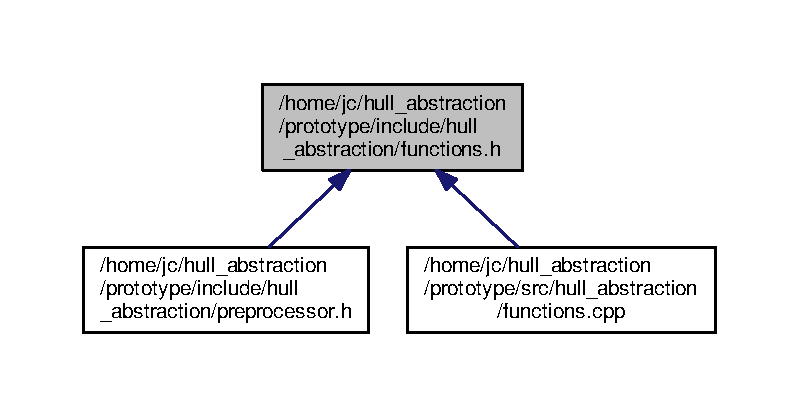
\includegraphics[width=350pt]{functions_8h__dep__incl}
\end{center}
\end{figure}
\subsection*{Namespaces}
\begin{DoxyCompactItemize}
\item 
 \hyperlink{namespacehull__abstraction}{hull\+\_\+abstraction}
\end{DoxyCompactItemize}
\subsection*{Functions}
\begin{DoxyCompactItemize}
\item 
double \hyperlink{namespacehull__abstraction_aee513dfed72060d83ec57c5909c9640e}{hull\+\_\+abstraction\+::compute\+Cloud\+Resolution} (pcl\+::\+Point\+Cloud$<$ pcl\+::\+Point\+X\+YZ $>$\+::Ptr cloud)
\item 
double \hyperlink{namespacehull__abstraction_aa0e1e236f8dd95c43e92d142cfc2754e}{hull\+\_\+abstraction\+::compute\+Cloud\+Resolution} (pcl\+::\+Point\+Cloud$<$ pcl\+::\+Point\+Normal $>$\+::Ptr cloud\+With\+Normals)
\item 
std\+::vector$<$ std\+::vector$<$ double $>$ $>$ \hyperlink{namespacehull__abstraction_a2e467ab4a24489895dc694bf4dec4ad1}{hull\+\_\+abstraction\+::compute\+A\+A\+BB} (pcl\+::\+Point\+Cloud$<$ pcl\+::\+Point\+X\+YZ $>$\+::Ptr cloud)
\item 
std\+::vector$<$ std\+::vector$<$ double $>$ $>$ \hyperlink{namespacehull__abstraction_ad0b9805fbf18fffc219231131cee1d9b}{hull\+\_\+abstraction\+::compute\+A\+A\+BB} (pcl\+::\+Point\+Cloud$<$ pcl\+::\+Point\+Normal $>$\+::Ptr cloud\+With\+Normals)
\end{DoxyCompactItemize}

\hypertarget{prototype_2include_2hull__abstraction_2preprocessor_8h}{}\section{/home/jc/hull\+\_\+abstraction/prototype/include/hull\+\_\+abstraction/preprocessor.h File Reference}
\label{prototype_2include_2hull__abstraction_2preprocessor_8h}\index{/home/jc/hull\+\_\+abstraction/prototype/include/hull\+\_\+abstraction/preprocessor.\+h@{/home/jc/hull\+\_\+abstraction/prototype/include/hull\+\_\+abstraction/preprocessor.\+h}}
{\ttfamily \#include $<$pcl/point\+\_\+types.\+h$>$}\\*
{\ttfamily \#include $<$pcl/filters/approximate\+\_\+voxel\+\_\+grid.\+h$>$}\\*
{\ttfamily \#include $<$pcl/features/normal\+\_\+3d.\+h$>$}\\*
{\ttfamily \#include $<$pcl/filters/statistical\+\_\+outlier\+\_\+removal.\+h$>$}\\*
{\ttfamily \#include $<$pcl/filters/passthrough.\+h$>$}\\*
{\ttfamily \#include $<$pcl/filters/conditional\+\_\+removal.\+h$>$}\\*
{\ttfamily \#include $<$pcl/filters/radius\+\_\+outlier\+\_\+removal.\+h$>$}\\*
{\ttfamily \#include $<$pcl/surface/mls.\+h$>$}\\*
{\ttfamily \#include \char`\"{}hull\+\_\+abstraction/functions.\+h\char`\"{}}\\*
Include dependency graph for preprocessor.\+h\+:\nopagebreak
\begin{figure}[H]
\begin{center}
\leavevmode
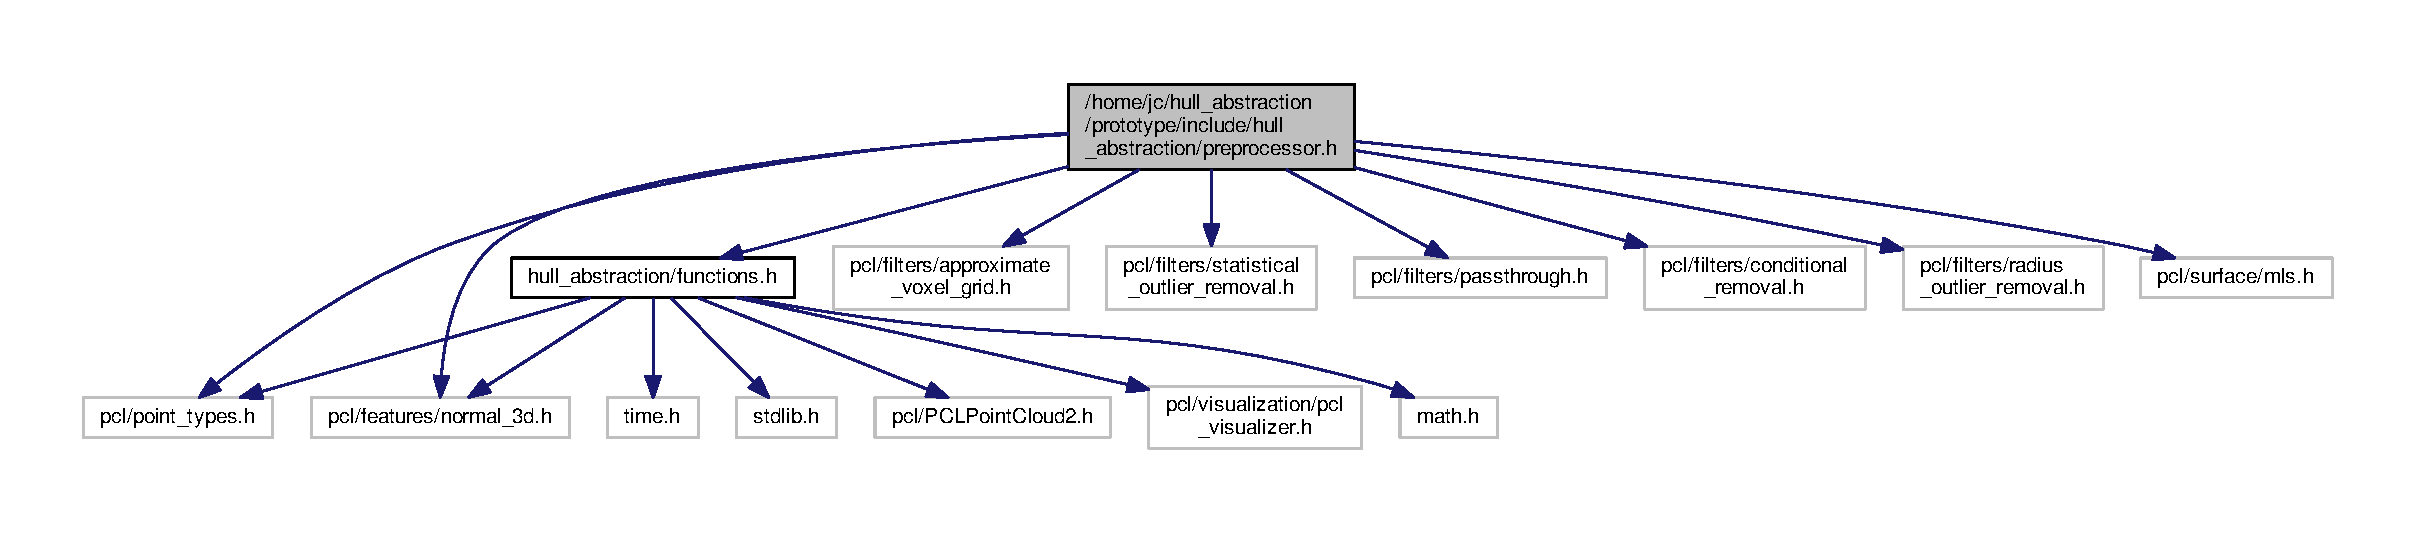
\includegraphics[width=350pt]{prototype_2include_2hull__abstraction_2preprocessor_8h__incl}
\end{center}
\end{figure}
\subsection*{Classes}
\begin{DoxyCompactItemize}
\item 
class \hyperlink{classhull__abstraction_1_1_preprocessor}{hull\+\_\+abstraction\+::\+Preprocessor}
\begin{DoxyCompactList}\small\item\em Class containing several preprocessing procedures. \end{DoxyCompactList}\end{DoxyCompactItemize}
\subsection*{Namespaces}
\begin{DoxyCompactItemize}
\item 
 \hyperlink{namespacehull__abstraction}{hull\+\_\+abstraction}
\end{DoxyCompactItemize}

\hypertarget{ros_2src_2hull__abstraction_2include_2hull__abstraction_2preprocessor_8h}{}\section{/home/jc/\+T\+H\+E\+S\+I\+S/hull\+\_\+abstraction/ros/src/hull\+\_\+abstraction/include/hull\+\_\+abstraction/preprocessor.h File Reference}
\label{ros_2src_2hull__abstraction_2include_2hull__abstraction_2preprocessor_8h}\index{/home/jc/\+T\+H\+E\+S\+I\+S/hull\+\_\+abstraction/ros/src/hull\+\_\+abstraction/include/hull\+\_\+abstraction/preprocessor.\+h@{/home/jc/\+T\+H\+E\+S\+I\+S/hull\+\_\+abstraction/ros/src/hull\+\_\+abstraction/include/hull\+\_\+abstraction/preprocessor.\+h}}


This file contains the declaration of the Preprocessor class.  


{\ttfamily \#include \char`\"{}pcl\+\_\+utilization/pcl\+\_\+utilization.\+h\char`\"{}}\\*
{\ttfamily \#include $<$pcl/point\+\_\+types.\+h$>$}\\*
{\ttfamily \#include $<$pcl/features/normal\+\_\+3d.\+h$>$}\\*
{\ttfamily \#include $<$pcl/filters/approximate\+\_\+voxel\+\_\+grid.\+h$>$}\\*
{\ttfamily \#include $<$pcl/filters/statistical\+\_\+outlier\+\_\+removal.\+h$>$}\\*
{\ttfamily \#include $<$pcl/filters/passthrough.\+h$>$}\\*
{\ttfamily \#include $<$pcl/filters/conditional\+\_\+removal.\+h$>$}\\*
{\ttfamily \#include $<$pcl/filters/radius\+\_\+outlier\+\_\+removal.\+h$>$}\\*
{\ttfamily \#include $<$pcl/surface/mls.\+h$>$}\\*
Include dependency graph for preprocessor.\+h\+:
\nopagebreak
\begin{figure}[H]
\begin{center}
\leavevmode
\includegraphics[width=350pt]{ros_2src_2hull__abstraction_2include_2hull__abstraction_2preprocessor_8h__incl}
\end{center}
\end{figure}
This graph shows which files directly or indirectly include this file\+:
\nopagebreak
\begin{figure}[H]
\begin{center}
\leavevmode
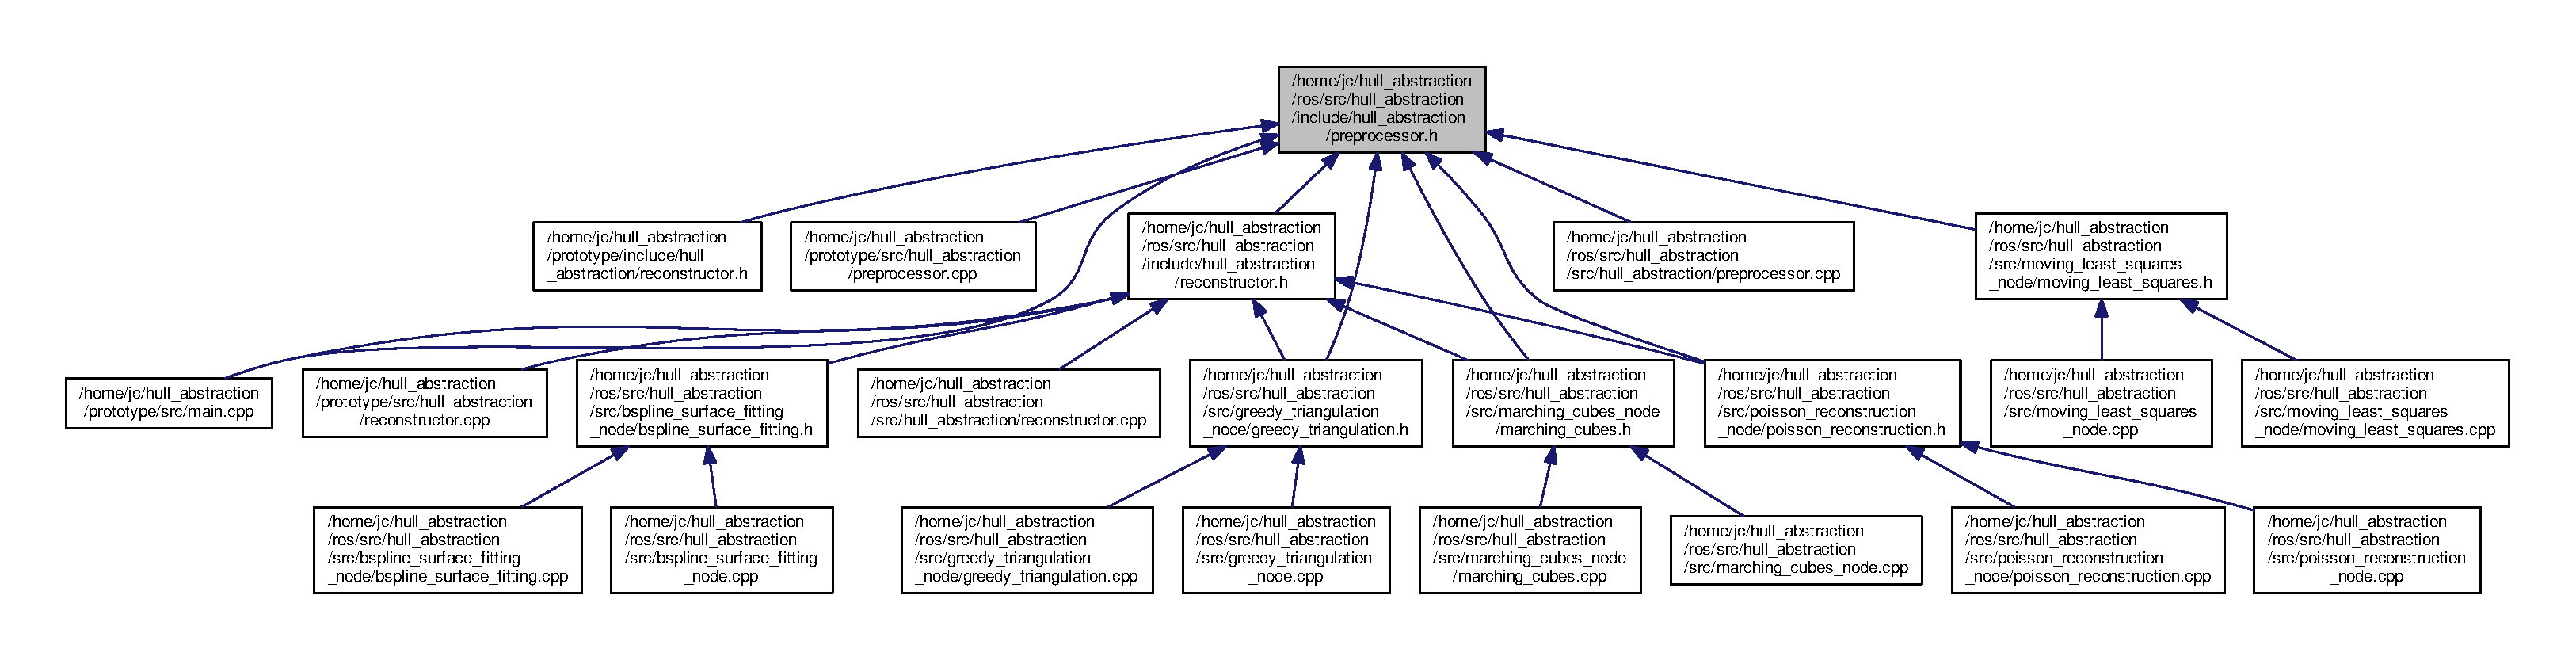
\includegraphics[width=350pt]{ros_2src_2hull__abstraction_2include_2hull__abstraction_2preprocessor_8h__dep__incl}
\end{center}
\end{figure}
\subsection*{Classes}
\begin{DoxyCompactItemize}
\item 
class \hyperlink{classhull__abstraction_1_1_preprocessor}{hull\+\_\+abstraction\+::\+Preprocessor}
\begin{DoxyCompactList}\small\item\em The \hyperlink{classhull__abstraction_1_1_preprocessor}{Preprocessor} class. \end{DoxyCompactList}\end{DoxyCompactItemize}
\subsection*{Namespaces}
\begin{DoxyCompactItemize}
\item 
 \hyperlink{namespacehull__abstraction}{hull\+\_\+abstraction}
\end{DoxyCompactItemize}


\subsection{Detailed Description}
This file contains the declaration of the Preprocessor class. 

\begin{DoxyAuthor}{Author}
Jiancong Zheng 
\end{DoxyAuthor}
\begin{DoxyDate}{Date}
2020-\/05-\/12 
\end{DoxyDate}

\hypertarget{prototype_2include_2hull__abstraction_2reconstructor_8h}{}\section{/home/jc/hull\+\_\+abstraction/prototype/include/hull\+\_\+abstraction/reconstructor.h File Reference}
\label{prototype_2include_2hull__abstraction_2reconstructor_8h}\index{/home/jc/hull\+\_\+abstraction/prototype/include/hull\+\_\+abstraction/reconstructor.\+h@{/home/jc/hull\+\_\+abstraction/prototype/include/hull\+\_\+abstraction/reconstructor.\+h}}
{\ttfamily \#include $<$pcl/surface/gp3.\+h$>$}\\*
{\ttfamily \#include $<$pcl/point\+\_\+types.\+h$>$}\\*
{\ttfamily \#include $<$pcl/\+P\+C\+L\+Point\+Cloud2.\+h$>$}\\*
{\ttfamily \#include $<$pcl/surface/poisson.\+h$>$}\\*
{\ttfamily \#include $<$pcl/surface/marching\+\_\+cubes\+\_\+hoppe.\+h$>$}\\*
{\ttfamily \#include \char`\"{}hull\+\_\+abstraction/preprocessor.\+h\char`\"{}}\\*
{\ttfamily \#include $<$pcl/surface/on\+\_\+nurbs/fitting\+\_\+surface\+\_\+tdm.\+h$>$}\\*
{\ttfamily \#include $<$pcl/surface/on\+\_\+nurbs/fitting\+\_\+curve\+\_\+2d\+\_\+asdm.\+h$>$}\\*
{\ttfamily \#include $<$pcl/surface/on\+\_\+nurbs/triangulation.\+h$>$}\\*
Include dependency graph for reconstructor.\+h\+:\nopagebreak
\begin{figure}[H]
\begin{center}
\leavevmode
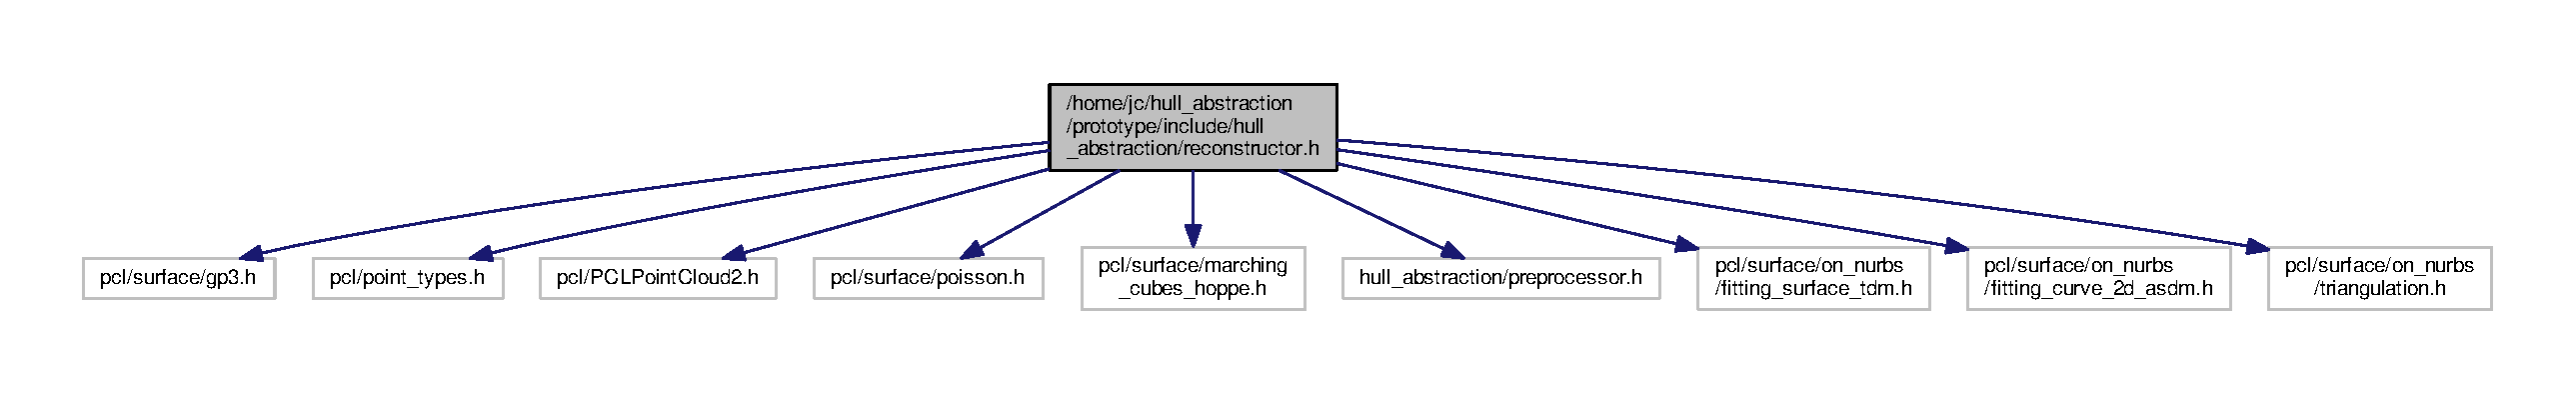
\includegraphics[width=350pt]{prototype_2include_2hull__abstraction_2reconstructor_8h__incl}
\end{center}
\end{figure}
\subsection*{Classes}
\begin{DoxyCompactItemize}
\item 
class \hyperlink{classhull__abstraction_1_1_reconstructor}{hull\+\_\+abstraction\+::\+Reconstructor}
\begin{DoxyCompactList}\small\item\em The \hyperlink{classhull__abstraction_1_1_reconstructor}{Reconstructor} class. \end{DoxyCompactList}\end{DoxyCompactItemize}
\subsection*{Namespaces}
\begin{DoxyCompactItemize}
\item 
 \hyperlink{namespacehull__abstraction}{hull\+\_\+abstraction}
\end{DoxyCompactItemize}

\hypertarget{ros_2src_2hull__abstraction_2include_2hull__abstraction_2reconstructor_8h}{}\section{/home/jc/\+T\+H\+E\+S\+I\+S/hull\+\_\+abstraction/ros/src/hull\+\_\+abstraction/include/hull\+\_\+abstraction/reconstructor.h File Reference}
\label{ros_2src_2hull__abstraction_2include_2hull__abstraction_2reconstructor_8h}\index{/home/jc/\+T\+H\+E\+S\+I\+S/hull\+\_\+abstraction/ros/src/hull\+\_\+abstraction/include/hull\+\_\+abstraction/reconstructor.\+h@{/home/jc/\+T\+H\+E\+S\+I\+S/hull\+\_\+abstraction/ros/src/hull\+\_\+abstraction/include/hull\+\_\+abstraction/reconstructor.\+h}}


This file contains the declaration of the Reconstructor class.  


{\ttfamily \#include \char`\"{}hull\+\_\+abstraction/preprocessor.\+h\char`\"{}}\\*
{\ttfamily \#include $<$pcl/point\+\_\+types.\+h$>$}\\*
{\ttfamily \#include $<$pcl/\+P\+C\+L\+Point\+Cloud2.\+h$>$}\\*
{\ttfamily \#include $<$pcl/surface/gp3.\+h$>$}\\*
{\ttfamily \#include $<$pcl/surface/poisson.\+h$>$}\\*
{\ttfamily \#include $<$pcl/surface/marching\+\_\+cubes\+\_\+hoppe.\+h$>$}\\*
{\ttfamily \#include $<$pcl/surface/on\+\_\+nurbs/fitting\+\_\+surface\+\_\+tdm.\+h$>$}\\*
{\ttfamily \#include $<$pcl/surface/on\+\_\+nurbs/fitting\+\_\+curve\+\_\+2d\+\_\+asdm.\+h$>$}\\*
{\ttfamily \#include $<$pcl/surface/on\+\_\+nurbs/triangulation.\+h$>$}\\*
Include dependency graph for reconstructor.\+h\+:
\nopagebreak
\begin{figure}[H]
\begin{center}
\leavevmode
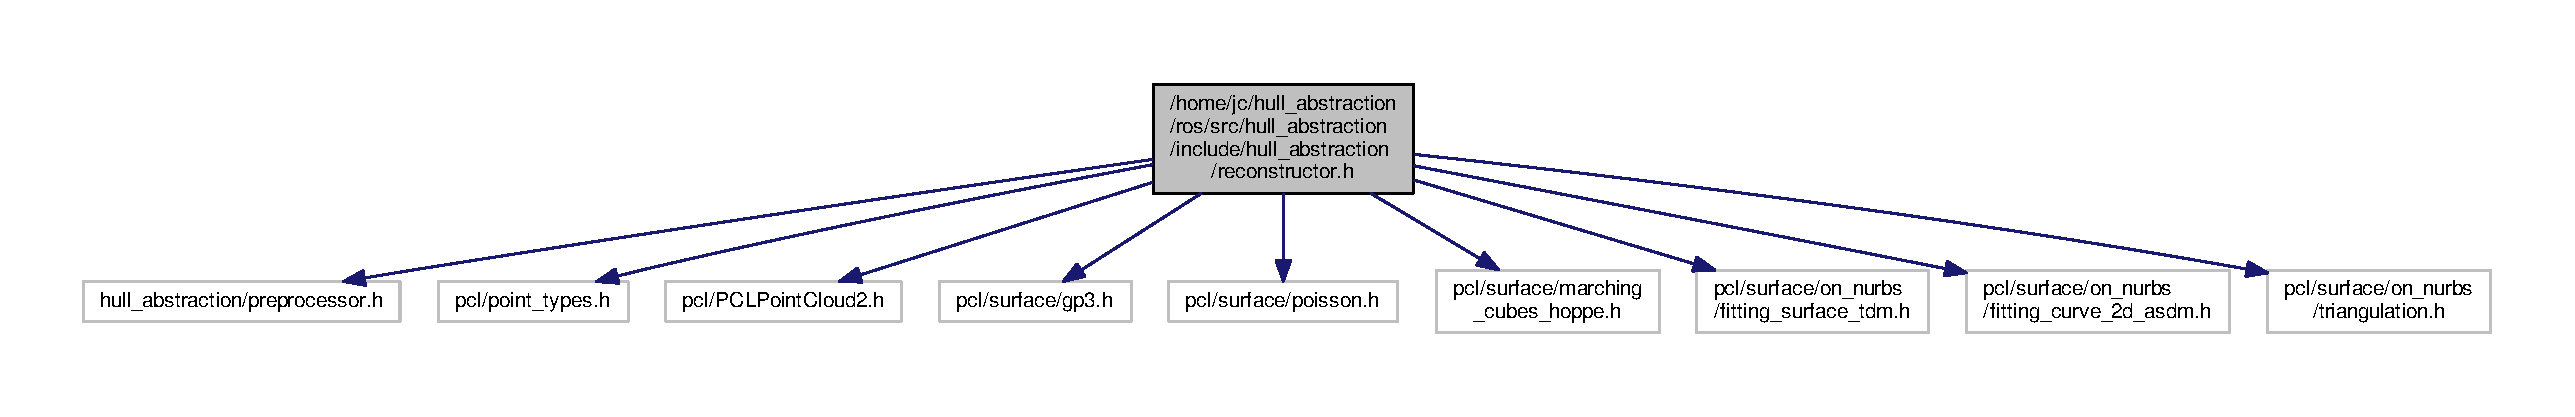
\includegraphics[width=350pt]{ros_2src_2hull__abstraction_2include_2hull__abstraction_2reconstructor_8h__incl}
\end{center}
\end{figure}
This graph shows which files directly or indirectly include this file\+:
\nopagebreak
\begin{figure}[H]
\begin{center}
\leavevmode
\includegraphics[width=350pt]{ros_2src_2hull__abstraction_2include_2hull__abstraction_2reconstructor_8h__dep__incl}
\end{center}
\end{figure}
\subsection*{Classes}
\begin{DoxyCompactItemize}
\item 
class \hyperlink{classhull__abstraction_1_1_reconstructor}{hull\+\_\+abstraction\+::\+Reconstructor}
\begin{DoxyCompactList}\small\item\em The \hyperlink{classhull__abstraction_1_1_reconstructor}{Reconstructor} class. \end{DoxyCompactList}\end{DoxyCompactItemize}
\subsection*{Namespaces}
\begin{DoxyCompactItemize}
\item 
 \hyperlink{namespacehull__abstraction}{hull\+\_\+abstraction}
\end{DoxyCompactItemize}


\subsection{Detailed Description}
This file contains the declaration of the Reconstructor class. 

\begin{DoxyAuthor}{Author}
Jiancong Zheng 
\end{DoxyAuthor}
\begin{DoxyDate}{Date}
2020-\/05-\/12 
\end{DoxyDate}

\hypertarget{functions_8cpp}{}\section{/home/jc/hull\+\_\+abstraction/prototype/src/hull\+\_\+abstraction/functions.cpp File Reference}
\label{functions_8cpp}\index{/home/jc/hull\+\_\+abstraction/prototype/src/hull\+\_\+abstraction/functions.\+cpp@{/home/jc/hull\+\_\+abstraction/prototype/src/hull\+\_\+abstraction/functions.\+cpp}}
{\ttfamily \#include \char`\"{}hull\+\_\+abstraction/functions.\+h\char`\"{}}\\*
Include dependency graph for functions.\+cpp\+:
\nopagebreak
\begin{figure}[H]
\begin{center}
\leavevmode
\includegraphics[width=350pt]{functions_8cpp__incl}
\end{center}
\end{figure}

\hypertarget{prototype_2src_2hull__abstraction_2preprocessor_8cpp}{}\section{/home/jc/hull\+\_\+abstraction/prototype/src/hull\+\_\+abstraction/preprocessor.cpp File Reference}
\label{prototype_2src_2hull__abstraction_2preprocessor_8cpp}\index{/home/jc/hull\+\_\+abstraction/prototype/src/hull\+\_\+abstraction/preprocessor.\+cpp@{/home/jc/hull\+\_\+abstraction/prototype/src/hull\+\_\+abstraction/preprocessor.\+cpp}}
{\ttfamily \#include \char`\"{}hull\+\_\+abstraction/preprocessor.\+h\char`\"{}}\\*
Include dependency graph for preprocessor.\+cpp\+:\nopagebreak
\begin{figure}[H]
\begin{center}
\leavevmode
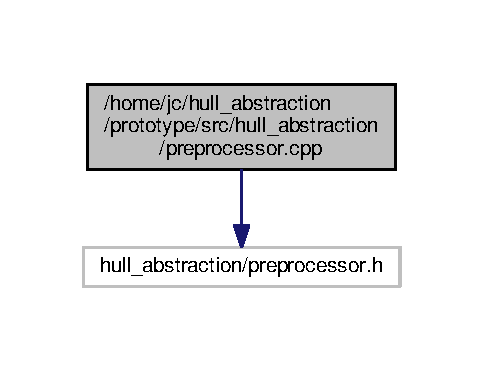
\includegraphics[width=232pt]{prototype_2src_2hull__abstraction_2preprocessor_8cpp__incl}
\end{center}
\end{figure}

\hypertarget{ros_2src_2hull__abstraction_2src_2hull__abstraction_2preprocessor_8cpp}{}\section{/home/jc/\+T\+H\+E\+S\+I\+S/hull\+\_\+abstraction/ros/src/hull\+\_\+abstraction/src/hull\+\_\+abstraction/preprocessor.cpp File Reference}
\label{ros_2src_2hull__abstraction_2src_2hull__abstraction_2preprocessor_8cpp}\index{/home/jc/\+T\+H\+E\+S\+I\+S/hull\+\_\+abstraction/ros/src/hull\+\_\+abstraction/src/hull\+\_\+abstraction/preprocessor.\+cpp@{/home/jc/\+T\+H\+E\+S\+I\+S/hull\+\_\+abstraction/ros/src/hull\+\_\+abstraction/src/hull\+\_\+abstraction/preprocessor.\+cpp}}
{\ttfamily \#include \char`\"{}hull\+\_\+abstraction/preprocessor.\+h\char`\"{}}\\*
Include dependency graph for preprocessor.\+cpp\+:
\nopagebreak
\begin{figure}[H]
\begin{center}
\leavevmode
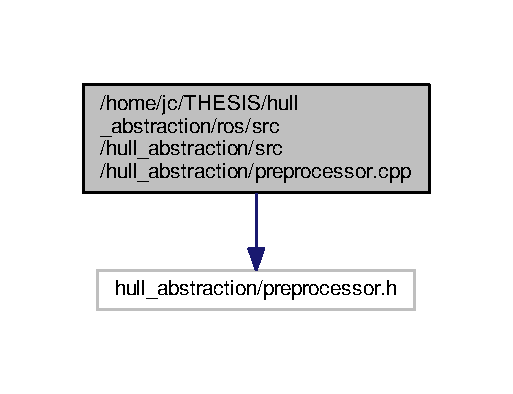
\includegraphics[width=246pt]{ros_2src_2hull__abstraction_2src_2hull__abstraction_2preprocessor_8cpp__incl}
\end{center}
\end{figure}

\hypertarget{prototype_2src_2hull__abstraction_2reconstructor_8cpp}{}\section{/home/jc/hull\+\_\+abstraction/prototype/src/hull\+\_\+abstraction/reconstructor.cpp File Reference}
\label{prototype_2src_2hull__abstraction_2reconstructor_8cpp}\index{/home/jc/hull\+\_\+abstraction/prototype/src/hull\+\_\+abstraction/reconstructor.\+cpp@{/home/jc/hull\+\_\+abstraction/prototype/src/hull\+\_\+abstraction/reconstructor.\+cpp}}
{\ttfamily \#include \char`\"{}hull\+\_\+abstraction/reconstructor.\+h\char`\"{}}\\*
Include dependency graph for reconstructor.\+cpp\+:\nopagebreak
\begin{figure}[H]
\begin{center}
\leavevmode
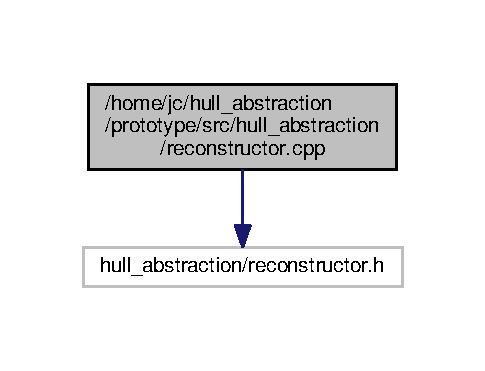
\includegraphics[width=233pt]{prototype_2src_2hull__abstraction_2reconstructor_8cpp__incl}
\end{center}
\end{figure}

\hypertarget{ros_2src_2hull__abstraction_2src_2hull__abstraction_2reconstructor_8cpp}{}\section{/home/jc/hull\+\_\+abstraction/ros/src/hull\+\_\+abstraction/src/hull\+\_\+abstraction/reconstructor.cpp File Reference}
\label{ros_2src_2hull__abstraction_2src_2hull__abstraction_2reconstructor_8cpp}\index{/home/jc/hull\+\_\+abstraction/ros/src/hull\+\_\+abstraction/src/hull\+\_\+abstraction/reconstructor.\+cpp@{/home/jc/hull\+\_\+abstraction/ros/src/hull\+\_\+abstraction/src/hull\+\_\+abstraction/reconstructor.\+cpp}}
{\ttfamily \#include \char`\"{}hull\+\_\+abstraction/reconstructor.\+h\char`\"{}}\\*
Include dependency graph for reconstructor.\+cpp\+:\nopagebreak
\begin{figure}[H]
\begin{center}
\leavevmode
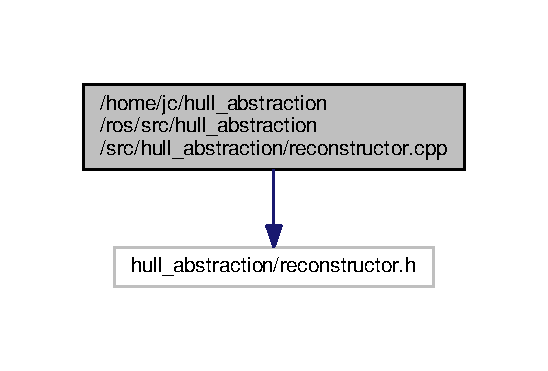
\includegraphics[width=263pt]{ros_2src_2hull__abstraction_2src_2hull__abstraction_2reconstructor_8cpp__incl}
\end{center}
\end{figure}

\hypertarget{main_8cpp}{}\section{/home/jc/hull\+\_\+abstraction/benchmark/src/main.cpp File Reference}
\label{main_8cpp}\index{/home/jc/hull\+\_\+abstraction/benchmark/src/main.\+cpp@{/home/jc/hull\+\_\+abstraction/benchmark/src/main.\+cpp}}
{\ttfamily \#include $<$iostream$>$}\\*
{\ttfamily \#include $<$string$>$}\\*
{\ttfamily \#include $<$pcl/io/ply\+\_\+io.\+h$>$}\\*
{\ttfamily \#include $<$pcl/io/pcd\+\_\+io.\+h$>$}\\*
{\ttfamily \#include $<$pcl/visualization/cloud\+\_\+viewer.\+h$>$}\\*
{\ttfamily \#include \char`\"{}hull\+\_\+abstraction/reconstructor.\+h\char`\"{}}\\*
{\ttfamily \#include \char`\"{}hull\+\_\+abstraction/preprocessor.\+h\char`\"{}}\\*
{\ttfamily \#include \char`\"{}benchmark/benchmark.\+h\char`\"{}}\\*
Include dependency graph for main.\+cpp\+:\nopagebreak
\begin{figure}[H]
\begin{center}
\leavevmode
\includegraphics[width=350pt]{main_8cpp__incl}
\end{center}
\end{figure}
\subsection*{Functions}
\begin{DoxyCompactItemize}
\item 
int \hyperlink{main_8cpp_ae66f6b31b5ad750f1fe042a706a4e3d4}{main} ()
\end{DoxyCompactItemize}


\subsection{Function Documentation}
\index{main.\+cpp@{main.\+cpp}!main@{main}}
\index{main@{main}!main.\+cpp@{main.\+cpp}}
\subsubsection[{\texorpdfstring{main()}{main()}}]{\setlength{\rightskip}{0pt plus 5cm}int main (
\begin{DoxyParamCaption}
{}
\end{DoxyParamCaption}
)}\hypertarget{main_8cpp_ae66f6b31b5ad750f1fe042a706a4e3d4}{}\label{main_8cpp_ae66f6b31b5ad750f1fe042a706a4e3d4}

\hypertarget{_r_e_a_d_m_e_8md}{}\section{/home/jc/hull\+\_\+abstraction/\+R\+E\+A\+D\+ME.md File Reference}
\label{_r_e_a_d_m_e_8md}\index{/home/jc/hull\+\_\+abstraction/\+R\+E\+A\+D\+M\+E.\+md@{/home/jc/hull\+\_\+abstraction/\+R\+E\+A\+D\+M\+E.\+md}}

\hypertarget{build_2atomic__configure_2__setup__util_8py}{}\section{/home/jc/\+T\+H\+E\+S\+I\+S/hull\+\_\+abstraction/ros/build/atomic\+\_\+configure/\+\_\+setup\+\_\+util.py File Reference}
\label{build_2atomic__configure_2__setup__util_8py}\index{/home/jc/\+T\+H\+E\+S\+I\+S/hull\+\_\+abstraction/ros/build/atomic\+\_\+configure/\+\_\+setup\+\_\+util.\+py@{/home/jc/\+T\+H\+E\+S\+I\+S/hull\+\_\+abstraction/ros/build/atomic\+\_\+configure/\+\_\+setup\+\_\+util.\+py}}
\subsection*{Namespaces}
\begin{DoxyCompactItemize}
\item 
 \hyperlink{namespace__setup__util}{\+\_\+setup\+\_\+util}
\end{DoxyCompactItemize}
\subsection*{Functions}
\begin{DoxyCompactItemize}
\item 
def \hyperlink{namespace__setup__util_af3030db6102b5aa35cd354a2fb6cca03}{\+\_\+setup\+\_\+util.\+rollback\+\_\+env\+\_\+variables} (environ, env\+\_\+var\+\_\+subfolders)
\item 
def \hyperlink{namespace__setup__util_af05661e87b3270e8bfd0fbc18a5eeec4}{\+\_\+setup\+\_\+util.\+\_\+rollback\+\_\+env\+\_\+variable} (environ, name, subfolders)
\item 
def \hyperlink{namespace__setup__util_ab2be07aa31918f1e1e34d6b7c4d66fcb}{\+\_\+setup\+\_\+util.\+\_\+get\+\_\+workspaces} (environ, include\+\_\+fuerte=False, include\+\_\+non\+\_\+existing=False)
\item 
def \hyperlink{namespace__setup__util_a832417d18b85bd1d276a87547e86f860}{\+\_\+setup\+\_\+util.\+prepend\+\_\+env\+\_\+variables} (environ, env\+\_\+var\+\_\+subfolders, workspaces)
\item 
def \hyperlink{namespace__setup__util_a74a1f8575ed82282d03f7795c9ba6e45}{\+\_\+setup\+\_\+util.\+\_\+prefix\+\_\+env\+\_\+variable} (environ, name, paths, subfolders)
\item 
def \hyperlink{namespace__setup__util_ad56c24837fa4eddc63c03fbc7035628f}{\+\_\+setup\+\_\+util.\+assignment} (key, value)
\item 
def \hyperlink{namespace__setup__util_abe8c95c4cfe8b1374dacd5f91d984353}{\+\_\+setup\+\_\+util.\+comment} (msg)
\item 
def \hyperlink{namespace__setup__util_ae78d86b2c4279f5b8b1acaa146c35802}{\+\_\+setup\+\_\+util.\+prepend} (environ, key, prefix)
\item 
def \hyperlink{namespace__setup__util_a73de35ca77f260af6691470342ab49ce}{\+\_\+setup\+\_\+util.\+find\+\_\+env\+\_\+hooks} (environ, cmake\+\_\+prefix\+\_\+path)
\item 
def \hyperlink{namespace__setup__util_a57d9ecb280810c9a5409d44aeb9d0a25}{\+\_\+setup\+\_\+util.\+\_\+parse\+\_\+arguments} (args=None)
\end{DoxyCompactItemize}
\subsection*{Variables}
\begin{DoxyCompactItemize}
\item 
string \hyperlink{namespace__setup__util_a3fa0ca5a460a71a43cbc3d4954ab1f10}{\+\_\+setup\+\_\+util.\+C\+A\+T\+K\+I\+N\+\_\+\+M\+A\+R\+K\+E\+R\+\_\+\+F\+I\+LE} = \textquotesingle{}.catkin\textquotesingle{}
\item 
\hyperlink{namespace__setup__util_ae9fca6a80a6923f4580be72f68fee325}{\+\_\+setup\+\_\+util.\+system} = platform.\+system()
\item 
tuple \hyperlink{namespace__setup__util_aecbb100ce6f94bb3c7e16d58fde05f96}{\+\_\+setup\+\_\+util.\+I\+S\+\_\+\+D\+A\+R\+W\+IN} = (system == \textquotesingle{}Darwin\textquotesingle{})
\item 
tuple \hyperlink{namespace__setup__util_a6fe69c2dbd92959b6651a28cbb846e6e}{\+\_\+setup\+\_\+util.\+I\+S\+\_\+\+W\+I\+N\+D\+O\+WS} = (system == \textquotesingle{}Windows\textquotesingle{})
\item 
list \hyperlink{namespace__setup__util_a7de27b8c021c888c6288a885f1e9afa9}{\+\_\+setup\+\_\+util.\+P\+A\+T\+H\+\_\+\+T\+O\+\_\+\+A\+D\+D\+\_\+\+S\+U\+F\+F\+IX} = \mbox{[}\textquotesingle{}bin\textquotesingle{}\mbox{]}
\item 
dictionary \hyperlink{namespace__setup__util_aa31804f1be8660156ce9394b33c68dc4}{\+\_\+setup\+\_\+util.\+E\+N\+V\+\_\+\+V\+A\+R\+\_\+\+S\+U\+B\+F\+O\+L\+D\+E\+RS}
\item 
\hyperlink{namespace__setup__util_a547963d07c6371df1c51b1384a2dec28}{\+\_\+setup\+\_\+util.\+args} = \+\_\+parse\+\_\+arguments()
\item 
\hyperlink{namespace__setup__util_acdce690b925de33d6249bbbfa1109d61}{\+\_\+setup\+\_\+util.\+e}
\item 
\hyperlink{namespace__setup__util_aea63a1b32cc79bc3d872ab7cb30dd07e}{\+\_\+setup\+\_\+util.\+file}
\item 
string \hyperlink{namespace__setup__util_a2a6756158bb4094ed7d259eb564d0578}{\+\_\+setup\+\_\+util.\+C\+M\+A\+K\+E\+\_\+\+P\+R\+E\+F\+I\+X\+\_\+\+P\+A\+TH} = \textquotesingle{}/opt/ros/kinetic\textquotesingle{}
\item 
\hyperlink{namespace__setup__util_a83d25140acd7788bbcb95843fe38e639}{\+\_\+setup\+\_\+util.\+base\+\_\+path} = os.\+path.\+dirname(\+\_\+\+\_\+file\+\_\+\+\_\+)
\item 
\hyperlink{namespace__setup__util_a9a935bdd9ee1aa0327161025bb18c136}{\+\_\+setup\+\_\+util.\+environ} = dict(os.\+environ)
\item 
list \hyperlink{namespace__setup__util_a8618d8be5f729d4c9696daa5e083a001}{\+\_\+setup\+\_\+util.\+lines} = \mbox{[}$\,$\mbox{]}
\end{DoxyCompactItemize}

\hypertarget{build_2catkin__generated_2installspace_2__setup__util_8py}{}\section{/home/jc/\+T\+H\+E\+S\+I\+S/hull\+\_\+abstraction/ros/build/catkin\+\_\+generated/installspace/\+\_\+setup\+\_\+util.py File Reference}
\label{build_2catkin__generated_2installspace_2__setup__util_8py}\index{/home/jc/\+T\+H\+E\+S\+I\+S/hull\+\_\+abstraction/ros/build/catkin\+\_\+generated/installspace/\+\_\+setup\+\_\+util.\+py@{/home/jc/\+T\+H\+E\+S\+I\+S/hull\+\_\+abstraction/ros/build/catkin\+\_\+generated/installspace/\+\_\+setup\+\_\+util.\+py}}
\subsection*{Namespaces}
\begin{DoxyCompactItemize}
\item 
 \hyperlink{namespace__setup__util}{\+\_\+setup\+\_\+util}
\end{DoxyCompactItemize}
\subsection*{Functions}
\begin{DoxyCompactItemize}
\item 
def \hyperlink{namespace__setup__util_af3030db6102b5aa35cd354a2fb6cca03}{\+\_\+setup\+\_\+util.\+rollback\+\_\+env\+\_\+variables} (environ, env\+\_\+var\+\_\+subfolders)
\item 
def \hyperlink{namespace__setup__util_af05661e87b3270e8bfd0fbc18a5eeec4}{\+\_\+setup\+\_\+util.\+\_\+rollback\+\_\+env\+\_\+variable} (environ, name, subfolders)
\item 
def \hyperlink{namespace__setup__util_ab2be07aa31918f1e1e34d6b7c4d66fcb}{\+\_\+setup\+\_\+util.\+\_\+get\+\_\+workspaces} (environ, include\+\_\+fuerte=False, include\+\_\+non\+\_\+existing=False)
\item 
def \hyperlink{namespace__setup__util_a832417d18b85bd1d276a87547e86f860}{\+\_\+setup\+\_\+util.\+prepend\+\_\+env\+\_\+variables} (environ, env\+\_\+var\+\_\+subfolders, workspaces)
\item 
def \hyperlink{namespace__setup__util_a74a1f8575ed82282d03f7795c9ba6e45}{\+\_\+setup\+\_\+util.\+\_\+prefix\+\_\+env\+\_\+variable} (environ, name, paths, subfolders)
\item 
def \hyperlink{namespace__setup__util_ad56c24837fa4eddc63c03fbc7035628f}{\+\_\+setup\+\_\+util.\+assignment} (key, value)
\item 
def \hyperlink{namespace__setup__util_abe8c95c4cfe8b1374dacd5f91d984353}{\+\_\+setup\+\_\+util.\+comment} (msg)
\item 
def \hyperlink{namespace__setup__util_ae78d86b2c4279f5b8b1acaa146c35802}{\+\_\+setup\+\_\+util.\+prepend} (environ, key, prefix)
\item 
def \hyperlink{namespace__setup__util_a73de35ca77f260af6691470342ab49ce}{\+\_\+setup\+\_\+util.\+find\+\_\+env\+\_\+hooks} (environ, cmake\+\_\+prefix\+\_\+path)
\item 
def \hyperlink{namespace__setup__util_a57d9ecb280810c9a5409d44aeb9d0a25}{\+\_\+setup\+\_\+util.\+\_\+parse\+\_\+arguments} (args=None)
\end{DoxyCompactItemize}

\hypertarget{devel_2__setup__util_8py}{}\section{/home/jc/\+T\+H\+E\+S\+I\+S/hull\+\_\+abstraction/ros/devel/\+\_\+setup\+\_\+util.py File Reference}
\label{devel_2__setup__util_8py}\index{/home/jc/\+T\+H\+E\+S\+I\+S/hull\+\_\+abstraction/ros/devel/\+\_\+setup\+\_\+util.\+py@{/home/jc/\+T\+H\+E\+S\+I\+S/hull\+\_\+abstraction/ros/devel/\+\_\+setup\+\_\+util.\+py}}
\subsection*{Namespaces}
\begin{DoxyCompactItemize}
\item 
 \hyperlink{namespace__setup__util}{\+\_\+setup\+\_\+util}
\end{DoxyCompactItemize}
\subsection*{Functions}
\begin{DoxyCompactItemize}
\item 
def \hyperlink{namespace__setup__util_af3030db6102b5aa35cd354a2fb6cca03}{\+\_\+setup\+\_\+util.\+rollback\+\_\+env\+\_\+variables} (environ, env\+\_\+var\+\_\+subfolders)
\item 
def \hyperlink{namespace__setup__util_af05661e87b3270e8bfd0fbc18a5eeec4}{\+\_\+setup\+\_\+util.\+\_\+rollback\+\_\+env\+\_\+variable} (environ, name, subfolders)
\item 
def \hyperlink{namespace__setup__util_ab2be07aa31918f1e1e34d6b7c4d66fcb}{\+\_\+setup\+\_\+util.\+\_\+get\+\_\+workspaces} (environ, include\+\_\+fuerte=False, include\+\_\+non\+\_\+existing=False)
\item 
def \hyperlink{namespace__setup__util_a832417d18b85bd1d276a87547e86f860}{\+\_\+setup\+\_\+util.\+prepend\+\_\+env\+\_\+variables} (environ, env\+\_\+var\+\_\+subfolders, workspaces)
\item 
def \hyperlink{namespace__setup__util_a74a1f8575ed82282d03f7795c9ba6e45}{\+\_\+setup\+\_\+util.\+\_\+prefix\+\_\+env\+\_\+variable} (environ, name, paths, subfolders)
\item 
def \hyperlink{namespace__setup__util_ad56c24837fa4eddc63c03fbc7035628f}{\+\_\+setup\+\_\+util.\+assignment} (key, value)
\item 
def \hyperlink{namespace__setup__util_abe8c95c4cfe8b1374dacd5f91d984353}{\+\_\+setup\+\_\+util.\+comment} (msg)
\item 
def \hyperlink{namespace__setup__util_ae78d86b2c4279f5b8b1acaa146c35802}{\+\_\+setup\+\_\+util.\+prepend} (environ, key, prefix)
\item 
def \hyperlink{namespace__setup__util_a73de35ca77f260af6691470342ab49ce}{\+\_\+setup\+\_\+util.\+find\+\_\+env\+\_\+hooks} (environ, cmake\+\_\+prefix\+\_\+path)
\item 
def \hyperlink{namespace__setup__util_a57d9ecb280810c9a5409d44aeb9d0a25}{\+\_\+setup\+\_\+util.\+\_\+parse\+\_\+arguments} (args=None)
\end{DoxyCompactItemize}

\hypertarget{generate__cached__setup_8py}{}\section{/home/jc/\+T\+H\+E\+S\+I\+S/hull\+\_\+abstraction/ros/build/catkin\+\_\+generated/generate\+\_\+cached\+\_\+setup.py File Reference}
\label{generate__cached__setup_8py}\index{/home/jc/\+T\+H\+E\+S\+I\+S/hull\+\_\+abstraction/ros/build/catkin\+\_\+generated/generate\+\_\+cached\+\_\+setup.\+py@{/home/jc/\+T\+H\+E\+S\+I\+S/hull\+\_\+abstraction/ros/build/catkin\+\_\+generated/generate\+\_\+cached\+\_\+setup.\+py}}
\subsection*{Namespaces}
\begin{DoxyCompactItemize}
\item 
 \hyperlink{namespacegenerate__cached__setup}{generate\+\_\+cached\+\_\+setup}
\end{DoxyCompactItemize}
\subsection*{Variables}
\begin{DoxyCompactItemize}
\item 
\hyperlink{namespacegenerate__cached__setup_a72579fd01529a79bab20d99291889d3f}{generate\+\_\+cached\+\_\+setup.\+python\+\_\+path} = os.\+path.\+join(workspace, \textquotesingle{}lib/python2.\+7/dist-\/packages\textquotesingle{})
\item 
\hyperlink{namespacegenerate__cached__setup_a52601295006f2366a311c4453d8f2f2e}{generate\+\_\+cached\+\_\+setup.\+code} = generate\+\_\+environment\+\_\+script(\textquotesingle{}/home/jc/T\+H\+E\+S\+IS/hull\+\_\+abstraction/ros/devel/env.\+sh\textquotesingle{})
\item 
string \hyperlink{namespacegenerate__cached__setup_a0265aee5075ee1eb701ff69c98ad6793}{generate\+\_\+cached\+\_\+setup.\+output\+\_\+filename} = \textquotesingle{}/home/jc/T\+H\+E\+S\+IS/hull\+\_\+abstraction/ros/build/catkin\+\_\+generated/setup\+\_\+cached.\+sh\textquotesingle{}
\item 
\hyperlink{namespacegenerate__cached__setup_a10081e5abedae9bd46dd91202096e789}{generate\+\_\+cached\+\_\+setup.\+mode} = os.\+stat(output\+\_\+filename).st\+\_\+mode
\end{DoxyCompactItemize}

\hypertarget{order__packages_8py}{}\section{/home/jc/hull\+\_\+abstraction/ros/build/catkin\+\_\+generated/order\+\_\+packages.py File Reference}
\label{order__packages_8py}\index{/home/jc/hull\+\_\+abstraction/ros/build/catkin\+\_\+generated/order\+\_\+packages.\+py@{/home/jc/hull\+\_\+abstraction/ros/build/catkin\+\_\+generated/order\+\_\+packages.\+py}}
\subsection*{Namespaces}
\begin{DoxyCompactItemize}
\item 
 \hyperlink{namespaceorder__packages}{order\+\_\+packages}
\end{DoxyCompactItemize}
\subsection*{Variables}
\begin{DoxyCompactItemize}
\item 
string \hyperlink{namespaceorder__packages_aff4fd297841de7fbddc2c0c33a6bab21}{order\+\_\+packages.\+source\+\_\+root\+\_\+dir} = \char`\"{}/home/jc/hull\+\_\+abstraction/ros/src\char`\"{}
\item 
string \hyperlink{namespaceorder__packages_a84450a73e77dbf3689293b97dcb697a4}{order\+\_\+packages.\+whitelisted\+\_\+packages} = \char`\"{}\char`\"{}
\item 
string \hyperlink{namespaceorder__packages_a29ea913f00c5a0e81d3c7688e7375507}{order\+\_\+packages.\+blacklisted\+\_\+packages} = \char`\"{}\char`\"{}
\item 
string \hyperlink{namespaceorder__packages_a11d102ff09fd2977b9075c4c722015d2}{order\+\_\+packages.\+underlay\+\_\+workspaces} = \char`\"{}/home/jc/hull\+\_\+abstraction/ros/devel;/opt/ros/kinetic\char`\"{}
\end{DoxyCompactItemize}

\hypertarget{pkg_8develspace_8context_8pc_8py}{}\section{/home/jc/\+T\+H\+E\+S\+I\+S/hull\+\_\+abstraction/ros/build/hull\+\_\+abstraction/catkin\+\_\+generated/pkg.develspace.\+context.\+pc.\+py File Reference}
\label{pkg_8develspace_8context_8pc_8py}\index{/home/jc/\+T\+H\+E\+S\+I\+S/hull\+\_\+abstraction/ros/build/hull\+\_\+abstraction/catkin\+\_\+generated/pkg.\+develspace.\+context.\+pc.\+py@{/home/jc/\+T\+H\+E\+S\+I\+S/hull\+\_\+abstraction/ros/build/hull\+\_\+abstraction/catkin\+\_\+generated/pkg.\+develspace.\+context.\+pc.\+py}}
\subsection*{Namespaces}
\begin{DoxyCompactItemize}
\item 
 \hyperlink{namespacepkg}{pkg}
\end{DoxyCompactItemize}
\subsection*{Variables}
\begin{DoxyCompactItemize}
\item 
string \hyperlink{namespacepkg_ae26c7a5a06b7d738f4d210ca449e6bee}{pkg.\+C\+A\+T\+K\+I\+N\+\_\+\+P\+A\+C\+K\+A\+G\+E\+\_\+\+P\+R\+E\+F\+IX} = \char`\"{}\char`\"{}
\item 
string \hyperlink{namespacepkg_a2760bf8266ff58da440f65ee91b203ab}{pkg.\+P\+R\+O\+J\+E\+C\+T\+\_\+\+P\+K\+G\+\_\+\+C\+O\+N\+F\+I\+G\+\_\+\+I\+N\+C\+L\+U\+D\+E\+\_\+\+D\+I\+RS} = \char`\"{}\char`\"{}
\item 
string \hyperlink{namespacepkg_a17c18447fad253ee1c0d76deec88028c}{pkg.\+P\+R\+O\+J\+E\+C\+T\+\_\+\+C\+A\+T\+K\+I\+N\+\_\+\+D\+E\+P\+E\+N\+DS} = \char`\"{}\char`\"{}
\item 
string \hyperlink{namespacepkg_a433e30cecb4a0123a7c4b384d168e336}{pkg.\+P\+K\+G\+\_\+\+C\+O\+N\+F\+I\+G\+\_\+\+L\+I\+B\+R\+A\+R\+I\+E\+S\+\_\+\+W\+I\+T\+H\+\_\+\+P\+R\+E\+F\+IX} = \char`\"{}\char`\"{}
\item 
string \hyperlink{namespacepkg_a7dfbe99257c26f5e4a3a5483995d9ddc}{pkg.\+P\+R\+O\+J\+E\+C\+T\+\_\+\+N\+A\+ME} = \char`\"{}hull\+\_\+abstraction\char`\"{}
\item 
string \hyperlink{namespacepkg_a3f0f1b4bc03c596525e025539ca4332f}{pkg.\+P\+R\+O\+J\+E\+C\+T\+\_\+\+S\+P\+A\+C\+E\+\_\+\+D\+IR} = \char`\"{}/home/jc/T\+H\+E\+S\+IS/hull\+\_\+abstraction/ros/devel\char`\"{}
\item 
string \hyperlink{namespacepkg_ab1037914b9286bb61855131c06149648}{pkg.\+P\+R\+O\+J\+E\+C\+T\+\_\+\+V\+E\+R\+S\+I\+ON} = \char`\"{}0.\+0.\+0\char`\"{}
\end{DoxyCompactItemize}

\hypertarget{pkg_8installspace_8context_8pc_8py}{}\section{/home/jc/hull\+\_\+abstraction/ros/build/hull\+\_\+abstraction/catkin\+\_\+generated/pkg.installspace.\+context.\+pc.\+py File Reference}
\label{pkg_8installspace_8context_8pc_8py}\index{/home/jc/hull\+\_\+abstraction/ros/build/hull\+\_\+abstraction/catkin\+\_\+generated/pkg.\+installspace.\+context.\+pc.\+py@{/home/jc/hull\+\_\+abstraction/ros/build/hull\+\_\+abstraction/catkin\+\_\+generated/pkg.\+installspace.\+context.\+pc.\+py}}
\subsection*{Namespaces}
\begin{DoxyCompactItemize}
\item 
 \hyperlink{namespacepkg}{pkg}
\end{DoxyCompactItemize}

\hypertarget{pcl__utilization_8h}{}\section{/home/jc/hull\+\_\+abstraction/ros/src/hull\+\_\+abstraction/include/pcl\+\_\+utilization/pcl\+\_\+utilization.h File Reference}
\label{pcl__utilization_8h}\index{/home/jc/hull\+\_\+abstraction/ros/src/hull\+\_\+abstraction/include/pcl\+\_\+utilization/pcl\+\_\+utilization.\+h@{/home/jc/hull\+\_\+abstraction/ros/src/hull\+\_\+abstraction/include/pcl\+\_\+utilization/pcl\+\_\+utilization.\+h}}


This file contains the declaration of P\+CL utilization methods.  


{\ttfamily \#include $<$ros/ros.\+h$>$}\\*
{\ttfamily \#include $<$sensor\+\_\+msgs/\+Point\+Cloud2.\+h$>$}\\*
{\ttfamily \#include $<$visualization\+\_\+msgs/\+Marker.\+h$>$}\\*
{\ttfamily \#include $<$Eigen/\+Core$>$}\\*
{\ttfamily \#include $<$pcl\+\_\+conversions/pcl\+\_\+conversions.\+h$>$}\\*
{\ttfamily \#include $<$pcl/point\+\_\+types.\+h$>$}\\*
{\ttfamily \#include $<$pcl/\+P\+C\+L\+Point\+Cloud2.\+h$>$}\\*
{\ttfamily \#include $<$pcl/common/centroid.\+h$>$}\\*
{\ttfamily \#include $<$pcl/search/kdtree.\+h$>$}\\*
Include dependency graph for pcl\+\_\+utilization.\+h\+:\nopagebreak
\begin{figure}[H]
\begin{center}
\leavevmode
\includegraphics[width=350pt]{pcl__utilization_8h__incl}
\end{center}
\end{figure}
This graph shows which files directly or indirectly include this file\+:\nopagebreak
\begin{figure}[H]
\begin{center}
\leavevmode
\includegraphics[width=350pt]{pcl__utilization_8h__dep__incl}
\end{center}
\end{figure}
\subsection*{Namespaces}
\begin{DoxyCompactItemize}
\item 
 \hyperlink{namespacepcl__utilization}{pcl\+\_\+utilization}
\end{DoxyCompactItemize}
\subsection*{Functions}
\begin{DoxyCompactItemize}
\item 
visualization\+\_\+msgs\+::\+Marker \hyperlink{namespacepcl__utilization_a051f0954371074c7331ba054d185950f}{pcl\+\_\+utilization\+::to\+Triangle\+List} (pcl\+::\+Polygon\+Mesh mesh)
\begin{DoxyCompactList}\small\item\em Convert a polygon mesh to a marker message with a triangle list. \end{DoxyCompactList}\item 
visualization\+\_\+msgs\+::\+Marker \hyperlink{namespacepcl__utilization_a1a3ffc60b638c2a551b02ba9a755d3f1}{pcl\+\_\+utilization\+::to\+Line\+List} (pcl\+::\+Polygon\+Mesh mesh)
\begin{DoxyCompactList}\small\item\em Convert a polygon mesh to a marker message with a line list. \end{DoxyCompactList}\item 
double \hyperlink{namespacepcl__utilization_ac199fc2120c5dce78fd87c2c1e0445d0}{pcl\+\_\+utilization\+::compute\+Cloud\+Resolution} (pcl\+::\+Point\+Cloud$<$ pcl\+::\+Point\+X\+YZ $>$\+::Ptr cloud)
\begin{DoxyCompactList}\small\item\em Computing the resolution of a point cloud. \end{DoxyCompactList}\item 
double \hyperlink{namespacepcl__utilization_a5fd7d53d77802f39bdec1098137e198a}{pcl\+\_\+utilization\+::compute\+Cloud\+Resolution} (pcl\+::\+Point\+Cloud$<$ pcl\+::\+Point\+Normal $>$\+::Ptr cloud\+\_\+with\+\_\+normals)
\begin{DoxyCompactList}\small\item\em Computing the resolution of a point cloud with normals. \end{DoxyCompactList}\end{DoxyCompactItemize}


\subsection{Detailed Description}
This file contains the declaration of P\+CL utilization methods. 

\begin{DoxyAuthor}{Author}
Jiancong Zheng 
\end{DoxyAuthor}
\begin{DoxyDate}{Date}
2020-\/05-\/12 
\end{DoxyDate}

\hypertarget{bspline__surface__fitting__node_8cpp}{}\section{/home/jc/hull\+\_\+abstraction/ros/src/hull\+\_\+abstraction/src/bspline\+\_\+surface\+\_\+fitting\+\_\+node.cpp File Reference}
\label{bspline__surface__fitting__node_8cpp}\index{/home/jc/hull\+\_\+abstraction/ros/src/hull\+\_\+abstraction/src/bspline\+\_\+surface\+\_\+fitting\+\_\+node.\+cpp@{/home/jc/hull\+\_\+abstraction/ros/src/hull\+\_\+abstraction/src/bspline\+\_\+surface\+\_\+fitting\+\_\+node.\+cpp}}
{\ttfamily \#include \char`\"{}bspline\+\_\+surface\+\_\+fitting\+\_\+node/bspline\+\_\+surface\+\_\+fitting.\+h\char`\"{}}\\*
Include dependency graph for bspline\+\_\+surface\+\_\+fitting\+\_\+node.\+cpp\+:\nopagebreak
\begin{figure}[H]
\begin{center}
\leavevmode
\includegraphics[width=350pt]{bspline__surface__fitting__node_8cpp__incl}
\end{center}
\end{figure}
\subsection*{Functions}
\begin{DoxyCompactItemize}
\item 
int \hyperlink{bspline__surface__fitting__node_8cpp_a3c04138a5bfe5d72780bb7e82a18e627}{main} (int argc, char $\ast$$\ast$argv)
\end{DoxyCompactItemize}


\subsection{Function Documentation}
\index{bspline\+\_\+surface\+\_\+fitting\+\_\+node.\+cpp@{bspline\+\_\+surface\+\_\+fitting\+\_\+node.\+cpp}!main@{main}}
\index{main@{main}!bspline\+\_\+surface\+\_\+fitting\+\_\+node.\+cpp@{bspline\+\_\+surface\+\_\+fitting\+\_\+node.\+cpp}}
\subsubsection[{\texorpdfstring{main(int argc, char $\ast$$\ast$argv)}{main(int argc, char **argv)}}]{\setlength{\rightskip}{0pt plus 5cm}int main (
\begin{DoxyParamCaption}
\item[{int}]{argc, }
\item[{char $\ast$$\ast$}]{argv}
\end{DoxyParamCaption}
)}\hypertarget{bspline__surface__fitting__node_8cpp_a3c04138a5bfe5d72780bb7e82a18e627}{}\label{bspline__surface__fitting__node_8cpp_a3c04138a5bfe5d72780bb7e82a18e627}

\hypertarget{bspline__surface__fitting_8cpp}{}\section{/home/jc/hull\+\_\+abstraction/ros/src/hull\+\_\+abstraction/src/bspline\+\_\+surface\+\_\+fitting\+\_\+node/bspline\+\_\+surface\+\_\+fitting.cpp File Reference}
\label{bspline__surface__fitting_8cpp}\index{/home/jc/hull\+\_\+abstraction/ros/src/hull\+\_\+abstraction/src/bspline\+\_\+surface\+\_\+fitting\+\_\+node/bspline\+\_\+surface\+\_\+fitting.\+cpp@{/home/jc/hull\+\_\+abstraction/ros/src/hull\+\_\+abstraction/src/bspline\+\_\+surface\+\_\+fitting\+\_\+node/bspline\+\_\+surface\+\_\+fitting.\+cpp}}
{\ttfamily \#include \char`\"{}bspline\+\_\+surface\+\_\+fitting.\+h\char`\"{}}\\*
Include dependency graph for bspline\+\_\+surface\+\_\+fitting.\+cpp\+:\nopagebreak
\begin{figure}[H]
\begin{center}
\leavevmode
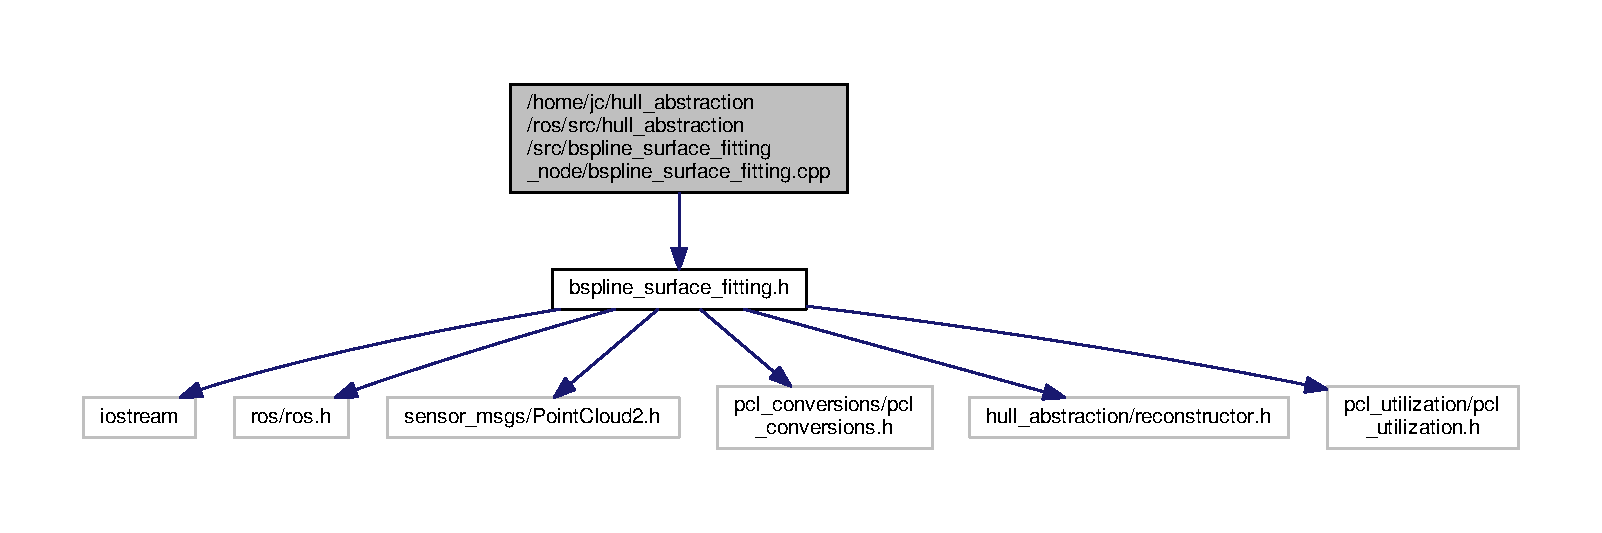
\includegraphics[width=350pt]{bspline__surface__fitting_8cpp__incl}
\end{center}
\end{figure}

\hypertarget{bspline__surface__fitting_8h}{}\section{/home/jc/hull\+\_\+abstraction/ros/src/hull\+\_\+abstraction/src/bspline\+\_\+surface\+\_\+fitting\+\_\+node/bspline\+\_\+surface\+\_\+fitting.h File Reference}
\label{bspline__surface__fitting_8h}\index{/home/jc/hull\+\_\+abstraction/ros/src/hull\+\_\+abstraction/src/bspline\+\_\+surface\+\_\+fitting\+\_\+node/bspline\+\_\+surface\+\_\+fitting.\+h@{/home/jc/hull\+\_\+abstraction/ros/src/hull\+\_\+abstraction/src/bspline\+\_\+surface\+\_\+fitting\+\_\+node/bspline\+\_\+surface\+\_\+fitting.\+h}}


Framework of b-\/spline surface fitting node.  


{\ttfamily \#include $<$iostream$>$}\\*
{\ttfamily \#include $<$ros/ros.\+h$>$}\\*
{\ttfamily \#include $<$sensor\+\_\+msgs/\+Point\+Cloud2.\+h$>$}\\*
{\ttfamily \#include $<$pcl\+\_\+conversions/pcl\+\_\+conversions.\+h$>$}\\*
{\ttfamily \#include \char`\"{}hull\+\_\+abstraction/reconstructor.\+h\char`\"{}}\\*
{\ttfamily \#include \char`\"{}pcl\+\_\+utilization/pcl\+\_\+utilization.\+h\char`\"{}}\\*
Include dependency graph for bspline\+\_\+surface\+\_\+fitting.\+h\+:\nopagebreak
\begin{figure}[H]
\begin{center}
\leavevmode
\includegraphics[width=350pt]{bspline__surface__fitting_8h__incl}
\end{center}
\end{figure}
This graph shows which files directly or indirectly include this file\+:\nopagebreak
\begin{figure}[H]
\begin{center}
\leavevmode
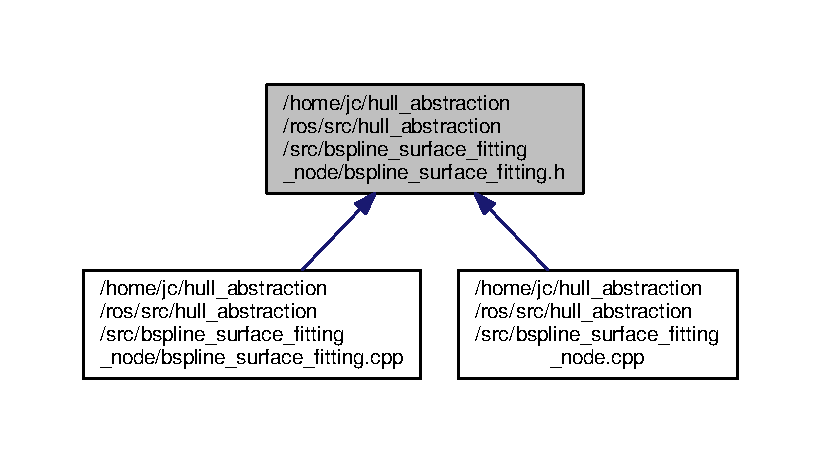
\includegraphics[width=350pt]{bspline__surface__fitting_8h__dep__incl}
\end{center}
\end{figure}
\subsection*{Classes}
\begin{DoxyCompactItemize}
\item 
class \hyperlink{classbspline__surface__fitting__node_1_1_bspline_surface_fitting}{bspline\+\_\+surface\+\_\+fitting\+\_\+node\+::\+Bspline\+Surface\+Fitting}
\begin{DoxyCompactList}\small\item\em Class utilizing B-\/spline surface fitting method. \end{DoxyCompactList}\end{DoxyCompactItemize}
\subsection*{Namespaces}
\begin{DoxyCompactItemize}
\item 
 \hyperlink{namespacebspline__surface__fitting__node}{bspline\+\_\+surface\+\_\+fitting\+\_\+node}
\end{DoxyCompactItemize}


\subsection{Detailed Description}
Framework of b-\/spline surface fitting node. 

\begin{DoxyRefDesc}{R\+O\+S Node}
\item[\hyperlink{ros_node__ros_node000001}{R\+O\+S Node}]bspline\+\_\+surface\+\_\+fitting\end{DoxyRefDesc}


\begin{DoxyAuthor}{Author}
Jiancong Zheng 
\end{DoxyAuthor}
\begin{DoxyDate}{Date}
2020-\/05-\/12
\end{DoxyDate}
This node subscribes a R\+OS topic to get an input point cloud and then perform b-\/spline surface fitting to generate a mesh. The result of b-\/spline surface fitting is published as a Marker message containing triangle lists. 
\hypertarget{display__mesh__node_8cpp}{}\section{/home/jc/hull\+\_\+abstraction/ros/src/hull\+\_\+abstraction/src/display\+\_\+mesh\+\_\+node.cpp File Reference}
\label{display__mesh__node_8cpp}\index{/home/jc/hull\+\_\+abstraction/ros/src/hull\+\_\+abstraction/src/display\+\_\+mesh\+\_\+node.\+cpp@{/home/jc/hull\+\_\+abstraction/ros/src/hull\+\_\+abstraction/src/display\+\_\+mesh\+\_\+node.\+cpp}}
{\ttfamily \#include \char`\"{}display\+\_\+mesh\+\_\+node/display\+\_\+mesh.\+h\char`\"{}}\\*
Include dependency graph for display\+\_\+mesh\+\_\+node.\+cpp\+:
\nopagebreak
\begin{figure}[H]
\begin{center}
\leavevmode
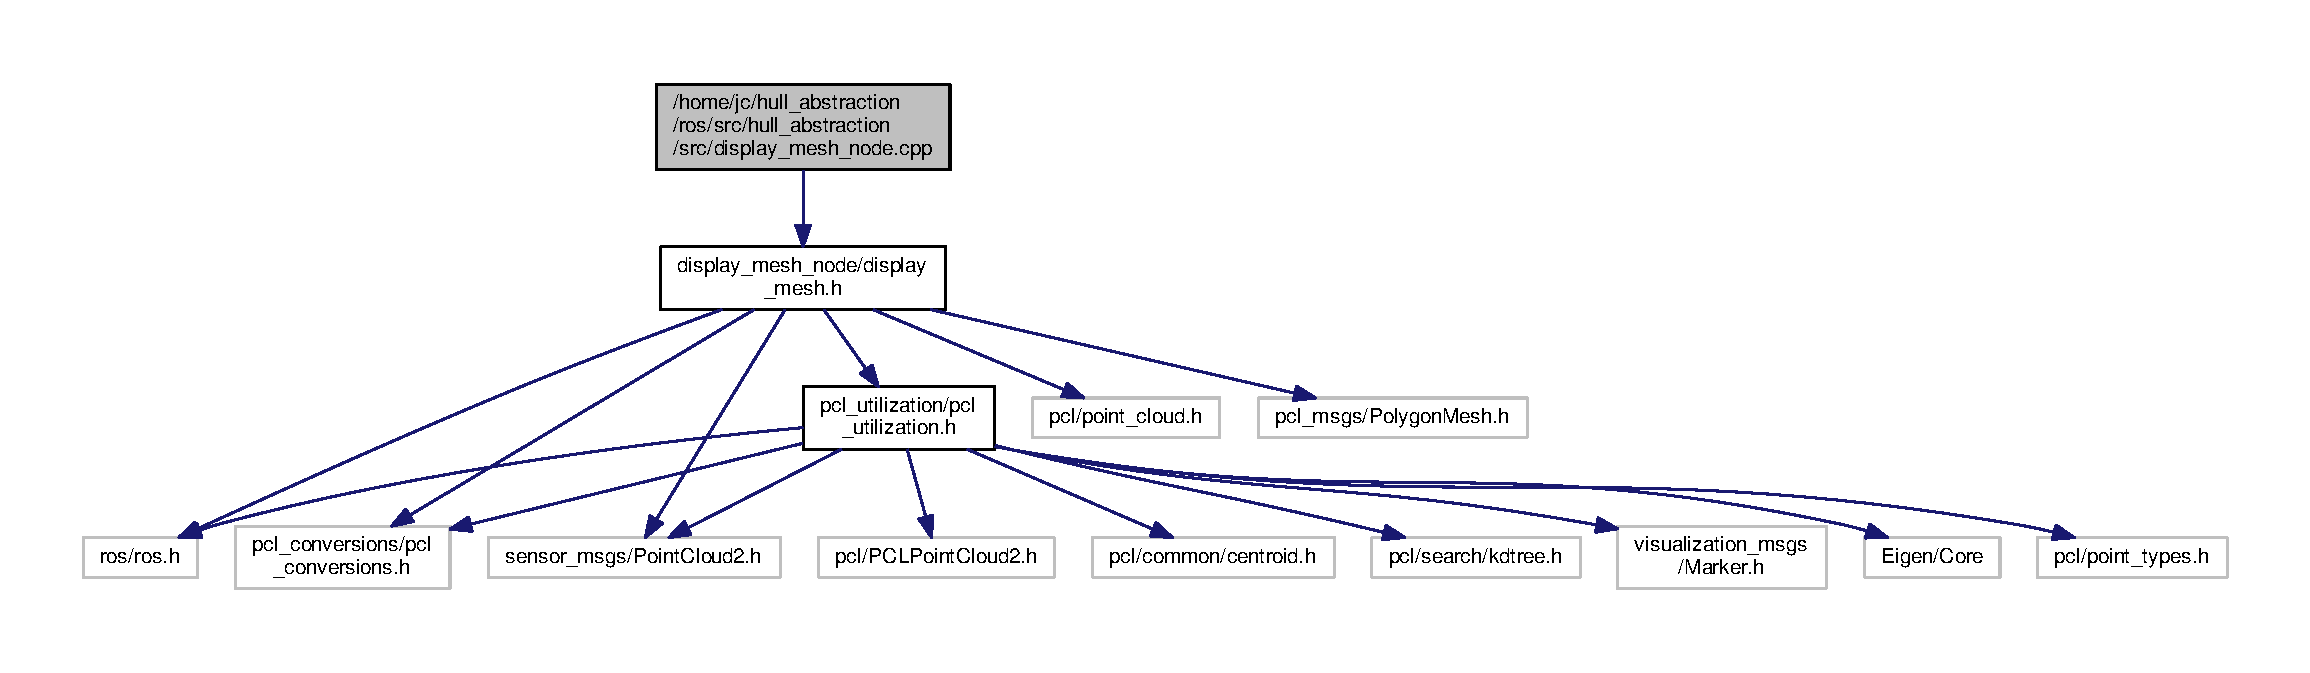
\includegraphics[width=350pt]{display__mesh__node_8cpp__incl}
\end{center}
\end{figure}
\subsection*{Functions}
\begin{DoxyCompactItemize}
\item 
int \hyperlink{display__mesh__node_8cpp_a3c04138a5bfe5d72780bb7e82a18e627}{main} (int argc, char $\ast$$\ast$argv)
\end{DoxyCompactItemize}


\subsection{Function Documentation}
\index{display\+\_\+mesh\+\_\+node.\+cpp@{display\+\_\+mesh\+\_\+node.\+cpp}!main@{main}}
\index{main@{main}!display\+\_\+mesh\+\_\+node.\+cpp@{display\+\_\+mesh\+\_\+node.\+cpp}}
\subsubsection[{\texorpdfstring{main(int argc, char $\ast$$\ast$argv)}{main(int argc, char **argv)}}]{\setlength{\rightskip}{0pt plus 5cm}int main (
\begin{DoxyParamCaption}
\item[{int}]{argc, }
\item[{char $\ast$$\ast$}]{argv}
\end{DoxyParamCaption}
)}\hypertarget{display__mesh__node_8cpp_a3c04138a5bfe5d72780bb7e82a18e627}{}\label{display__mesh__node_8cpp_a3c04138a5bfe5d72780bb7e82a18e627}

\hypertarget{display__mesh_8cpp}{}\section{/home/jc/hull\+\_\+abstraction/ros/src/hull\+\_\+abstraction/src/display\+\_\+mesh\+\_\+node/display\+\_\+mesh.cpp File Reference}
\label{display__mesh_8cpp}\index{/home/jc/hull\+\_\+abstraction/ros/src/hull\+\_\+abstraction/src/display\+\_\+mesh\+\_\+node/display\+\_\+mesh.\+cpp@{/home/jc/hull\+\_\+abstraction/ros/src/hull\+\_\+abstraction/src/display\+\_\+mesh\+\_\+node/display\+\_\+mesh.\+cpp}}
{\ttfamily \#include \char`\"{}display\+\_\+mesh.\+h\char`\"{}}\\*
Include dependency graph for display\+\_\+mesh.\+cpp\+:
\nopagebreak
\begin{figure}[H]
\begin{center}
\leavevmode
\includegraphics[width=350pt]{display__mesh_8cpp__incl}
\end{center}
\end{figure}

\hypertarget{display__mesh_8h}{}\section{/home/jc/\+T\+H\+E\+S\+I\+S/hull\+\_\+abstraction/ros/src/hull\+\_\+abstraction/src/display\+\_\+mesh\+\_\+node/display\+\_\+mesh.h File Reference}
\label{display__mesh_8h}\index{/home/jc/\+T\+H\+E\+S\+I\+S/hull\+\_\+abstraction/ros/src/hull\+\_\+abstraction/src/display\+\_\+mesh\+\_\+node/display\+\_\+mesh.\+h@{/home/jc/\+T\+H\+E\+S\+I\+S/hull\+\_\+abstraction/ros/src/hull\+\_\+abstraction/src/display\+\_\+mesh\+\_\+node/display\+\_\+mesh.\+h}}


Framework of node for displaying polygon meshes.  


{\ttfamily \#include $<$ros/ros.\+h$>$}\\*
{\ttfamily \#include $<$pcl/point\+\_\+cloud.\+h$>$}\\*
{\ttfamily \#include $<$pcl\+\_\+conversions/pcl\+\_\+conversions.\+h$>$}\\*
{\ttfamily \#include $<$pcl\+\_\+msgs/\+Polygon\+Mesh.\+h$>$}\\*
{\ttfamily \#include $<$sensor\+\_\+msgs/\+Point\+Cloud2.\+h$>$}\\*
{\ttfamily \#include \char`\"{}pcl\+\_\+utilization/pcl\+\_\+utilization.\+h\char`\"{}}\\*
Include dependency graph for display\+\_\+mesh.\+h\+:
\nopagebreak
\begin{figure}[H]
\begin{center}
\leavevmode
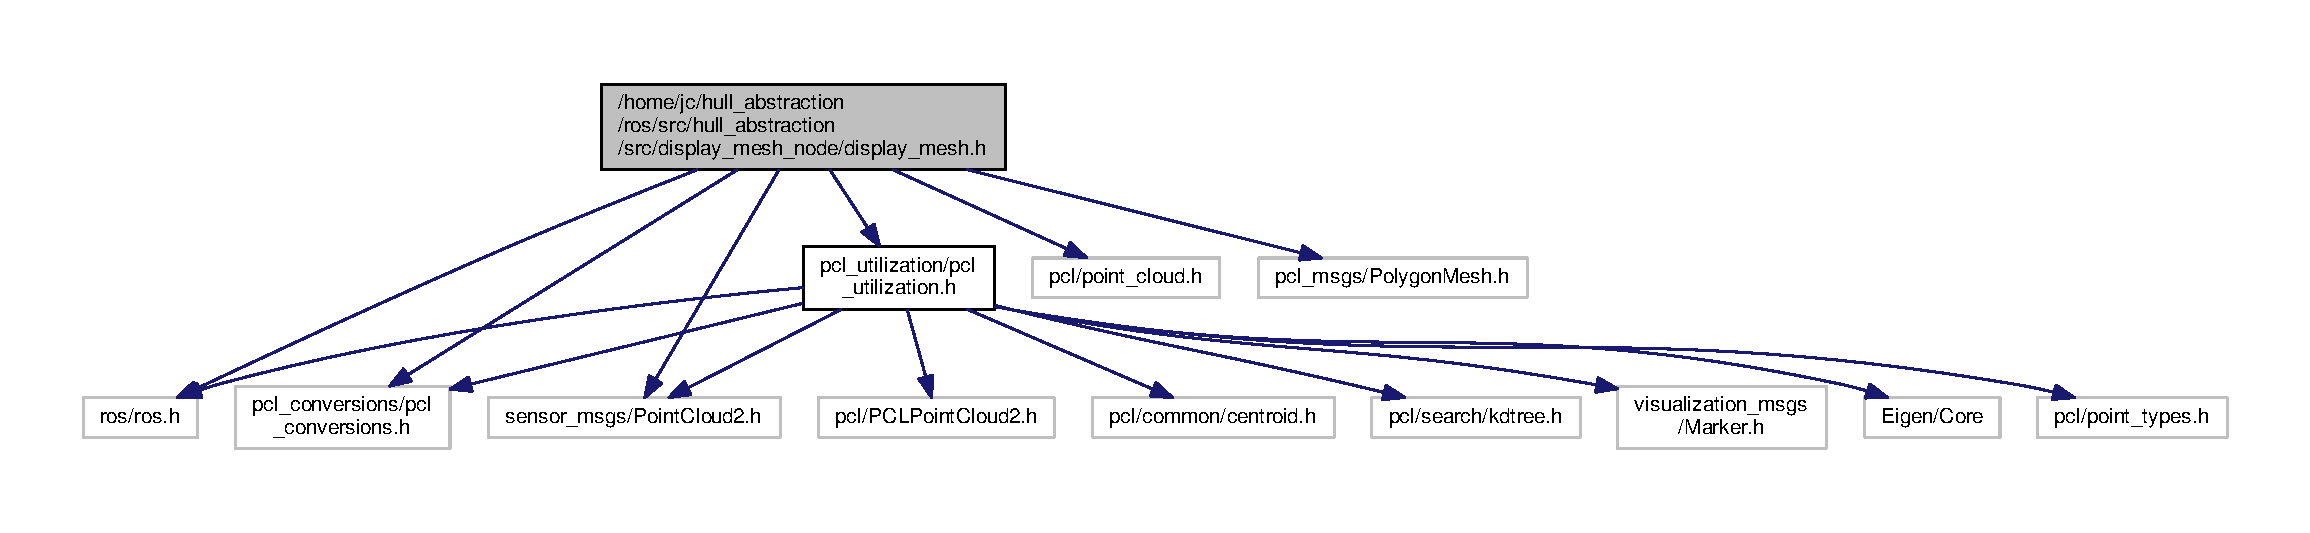
\includegraphics[width=350pt]{display__mesh_8h__incl}
\end{center}
\end{figure}
This graph shows which files directly or indirectly include this file\+:
\nopagebreak
\begin{figure}[H]
\begin{center}
\leavevmode
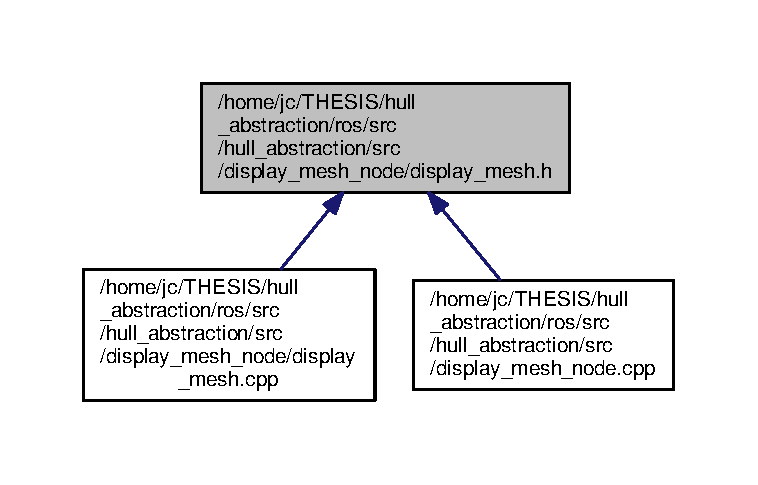
\includegraphics[width=350pt]{display__mesh_8h__dep__incl}
\end{center}
\end{figure}
\subsection*{Classes}
\begin{DoxyCompactItemize}
\item 
class \hyperlink{classdisplay__mesh_1_1_display_mesh}{display\+\_\+mesh\+::\+Display\+Mesh}
\begin{DoxyCompactList}\small\item\em Class for displaying mesh in R\+V\+IZ. \end{DoxyCompactList}\end{DoxyCompactItemize}
\subsection*{Namespaces}
\begin{DoxyCompactItemize}
\item 
 \hyperlink{namespacedisplay__mesh}{display\+\_\+mesh}
\end{DoxyCompactItemize}


\subsection{Detailed Description}
Framework of node for displaying polygon meshes. 

\begin{DoxyRefDesc}{R\+O\+S Node}
\item[\hyperlink{ros_node__ros_node000002}{R\+O\+S Node}]display\+\_\+mesh\+\_\+node\end{DoxyRefDesc}


\begin{DoxyAuthor}{Author}
Jiancong Zheng 
\end{DoxyAuthor}
\begin{DoxyDate}{Date}
2020-\/05-\/18
\end{DoxyDate}
This node subscribes topic which contains mseeage for polygon mesh and then process the mesh for display in R\+V\+IZ. 
\hypertarget{greedy__triangulation__node_8cpp}{}\section{/home/jc/hull\+\_\+abstraction/ros/src/hull\+\_\+abstraction/src/greedy\+\_\+triangulation\+\_\+node.cpp File Reference}
\label{greedy__triangulation__node_8cpp}\index{/home/jc/hull\+\_\+abstraction/ros/src/hull\+\_\+abstraction/src/greedy\+\_\+triangulation\+\_\+node.\+cpp@{/home/jc/hull\+\_\+abstraction/ros/src/hull\+\_\+abstraction/src/greedy\+\_\+triangulation\+\_\+node.\+cpp}}
{\ttfamily \#include \char`\"{}greedy\+\_\+triangulation\+\_\+node/greedy\+\_\+triangulation.\+h\char`\"{}}\\*
Include dependency graph for greedy\+\_\+triangulation\+\_\+node.\+cpp\+:\nopagebreak
\begin{figure}[H]
\begin{center}
\leavevmode
\includegraphics[width=350pt]{greedy__triangulation__node_8cpp__incl}
\end{center}
\end{figure}
\subsection*{Functions}
\begin{DoxyCompactItemize}
\item 
int \hyperlink{greedy__triangulation__node_8cpp_a3c04138a5bfe5d72780bb7e82a18e627}{main} (int argc, char $\ast$$\ast$argv)
\end{DoxyCompactItemize}


\subsection{Function Documentation}
\index{greedy\+\_\+triangulation\+\_\+node.\+cpp@{greedy\+\_\+triangulation\+\_\+node.\+cpp}!main@{main}}
\index{main@{main}!greedy\+\_\+triangulation\+\_\+node.\+cpp@{greedy\+\_\+triangulation\+\_\+node.\+cpp}}
\subsubsection[{\texorpdfstring{main(int argc, char $\ast$$\ast$argv)}{main(int argc, char **argv)}}]{\setlength{\rightskip}{0pt plus 5cm}int main (
\begin{DoxyParamCaption}
\item[{int}]{argc, }
\item[{char $\ast$$\ast$}]{argv}
\end{DoxyParamCaption}
)}\hypertarget{greedy__triangulation__node_8cpp_a3c04138a5bfe5d72780bb7e82a18e627}{}\label{greedy__triangulation__node_8cpp_a3c04138a5bfe5d72780bb7e82a18e627}

\hypertarget{greedy__triangulation_8cpp}{}\section{/home/jc/hull\+\_\+abstraction/ros/src/hull\+\_\+abstraction/src/greedy\+\_\+triangulation\+\_\+node/greedy\+\_\+triangulation.cpp File Reference}
\label{greedy__triangulation_8cpp}\index{/home/jc/hull\+\_\+abstraction/ros/src/hull\+\_\+abstraction/src/greedy\+\_\+triangulation\+\_\+node/greedy\+\_\+triangulation.\+cpp@{/home/jc/hull\+\_\+abstraction/ros/src/hull\+\_\+abstraction/src/greedy\+\_\+triangulation\+\_\+node/greedy\+\_\+triangulation.\+cpp}}
{\ttfamily \#include \char`\"{}greedy\+\_\+triangulation.\+h\char`\"{}}\\*
Include dependency graph for greedy\+\_\+triangulation.\+cpp\+:\nopagebreak
\begin{figure}[H]
\begin{center}
\leavevmode
\includegraphics[width=350pt]{greedy__triangulation_8cpp__incl}
\end{center}
\end{figure}

\hypertarget{greedy__triangulation_8h}{}\section{/home/jc/hull\+\_\+abstraction/ros/src/hull\+\_\+abstraction/src/greedy\+\_\+triangulation\+\_\+node/greedy\+\_\+triangulation.h File Reference}
\label{greedy__triangulation_8h}\index{/home/jc/hull\+\_\+abstraction/ros/src/hull\+\_\+abstraction/src/greedy\+\_\+triangulation\+\_\+node/greedy\+\_\+triangulation.\+h@{/home/jc/hull\+\_\+abstraction/ros/src/hull\+\_\+abstraction/src/greedy\+\_\+triangulation\+\_\+node/greedy\+\_\+triangulation.\+h}}


Framework of greedy triangulation node.  


{\ttfamily \#include $<$iostream$>$}\\*
{\ttfamily \#include $<$ros/ros.\+h$>$}\\*
{\ttfamily \#include $<$sensor\+\_\+msgs/\+Point\+Cloud2.\+h$>$}\\*
{\ttfamily \#include $<$pcl\+\_\+msgs/\+Polygon\+Mesh.\+h$>$}\\*
{\ttfamily \#include $<$pcl\+\_\+conversions/pcl\+\_\+conversions.\+h$>$}\\*
{\ttfamily \#include \char`\"{}hull\+\_\+abstraction/reconstructor.\+h\char`\"{}}\\*
{\ttfamily \#include \char`\"{}hull\+\_\+abstraction/preprocessor.\+h\char`\"{}}\\*
{\ttfamily \#include \char`\"{}pcl\+\_\+utilization/pcl\+\_\+utilization.\+h\char`\"{}}\\*
Include dependency graph for greedy\+\_\+triangulation.\+h\+:\nopagebreak
\begin{figure}[H]
\begin{center}
\leavevmode
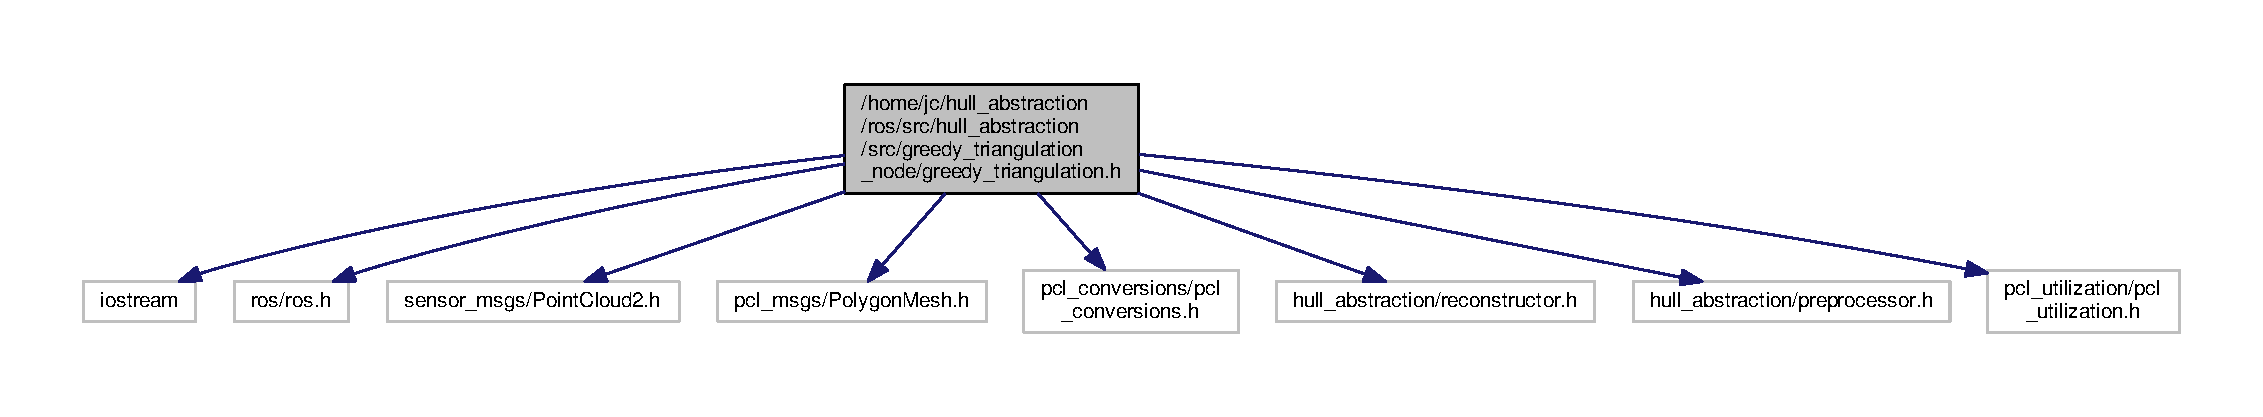
\includegraphics[width=350pt]{greedy__triangulation_8h__incl}
\end{center}
\end{figure}
This graph shows which files directly or indirectly include this file\+:\nopagebreak
\begin{figure}[H]
\begin{center}
\leavevmode
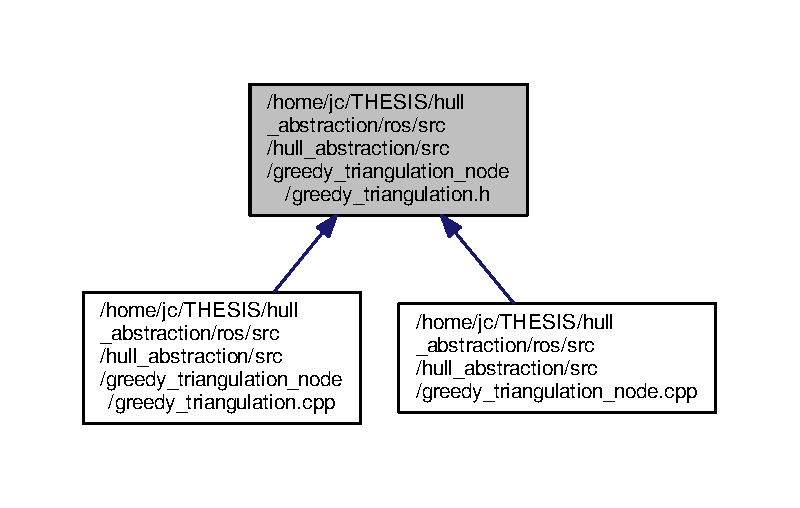
\includegraphics[width=350pt]{greedy__triangulation_8h__dep__incl}
\end{center}
\end{figure}
\subsection*{Classes}
\begin{DoxyCompactItemize}
\item 
class \hyperlink{classgreedy__triangulation__node_1_1_greedy_triangulation}{greedy\+\_\+triangulation\+\_\+node\+::\+Greedy\+Triangulation}
\begin{DoxyCompactList}\small\item\em Class utilizing greedy triangulation method. \end{DoxyCompactList}\end{DoxyCompactItemize}
\subsection*{Namespaces}
\begin{DoxyCompactItemize}
\item 
 \hyperlink{namespacegreedy__triangulation__node}{greedy\+\_\+triangulation\+\_\+node}
\end{DoxyCompactItemize}


\subsection{Detailed Description}
Framework of greedy triangulation node. 

\begin{DoxyRefDesc}{R\+O\+S Node}
\item[\hyperlink{ros_node__ros_node000002}{R\+O\+S Node}]greedy\+\_\+triangulation\end{DoxyRefDesc}


\begin{DoxyAuthor}{Author}
Jiancong Zheng 
\end{DoxyAuthor}
\begin{DoxyDate}{Date}
2020-\/05-\/12
\end{DoxyDate}
This node subscribes a R\+OS topic to get an input point cloud and then utilize greedy triangulation algorithm to generate a mesh. The result of greedy triangulation is published as a Marker message with triangle lists. 
\hypertarget{load__pcd__node_8cpp}{}\section{/home/jc/hull\+\_\+abstraction/ros/src/hull\+\_\+abstraction/src/load\+\_\+pcd\+\_\+node.cpp File Reference}
\label{load__pcd__node_8cpp}\index{/home/jc/hull\+\_\+abstraction/ros/src/hull\+\_\+abstraction/src/load\+\_\+pcd\+\_\+node.\+cpp@{/home/jc/hull\+\_\+abstraction/ros/src/hull\+\_\+abstraction/src/load\+\_\+pcd\+\_\+node.\+cpp}}
{\ttfamily \#include \char`\"{}load\+\_\+pcd\+\_\+node/load\+\_\+pcd.\+h\char`\"{}}\\*
Include dependency graph for load\+\_\+pcd\+\_\+node.\+cpp\+:\nopagebreak
\begin{figure}[H]
\begin{center}
\leavevmode
\includegraphics[width=350pt]{load__pcd__node_8cpp__incl}
\end{center}
\end{figure}
\subsection*{Functions}
\begin{DoxyCompactItemize}
\item 
int \hyperlink{load__pcd__node_8cpp_a3c04138a5bfe5d72780bb7e82a18e627}{main} (int argc, char $\ast$$\ast$argv)
\end{DoxyCompactItemize}


\subsection{Function Documentation}
\index{load\+\_\+pcd\+\_\+node.\+cpp@{load\+\_\+pcd\+\_\+node.\+cpp}!main@{main}}
\index{main@{main}!load\+\_\+pcd\+\_\+node.\+cpp@{load\+\_\+pcd\+\_\+node.\+cpp}}
\subsubsection[{\texorpdfstring{main(int argc, char $\ast$$\ast$argv)}{main(int argc, char **argv)}}]{\setlength{\rightskip}{0pt plus 5cm}int main (
\begin{DoxyParamCaption}
\item[{int}]{argc, }
\item[{char $\ast$$\ast$}]{argv}
\end{DoxyParamCaption}
)}\hypertarget{load__pcd__node_8cpp_a3c04138a5bfe5d72780bb7e82a18e627}{}\label{load__pcd__node_8cpp_a3c04138a5bfe5d72780bb7e82a18e627}

\hypertarget{load__pcd_8cpp}{}\section{/home/jc/\+T\+H\+E\+S\+I\+S/hull\+\_\+abstraction/ros/src/hull\+\_\+abstraction/src/load\+\_\+pcd\+\_\+node/load\+\_\+pcd.cpp File Reference}
\label{load__pcd_8cpp}\index{/home/jc/\+T\+H\+E\+S\+I\+S/hull\+\_\+abstraction/ros/src/hull\+\_\+abstraction/src/load\+\_\+pcd\+\_\+node/load\+\_\+pcd.\+cpp@{/home/jc/\+T\+H\+E\+S\+I\+S/hull\+\_\+abstraction/ros/src/hull\+\_\+abstraction/src/load\+\_\+pcd\+\_\+node/load\+\_\+pcd.\+cpp}}
{\ttfamily \#include \char`\"{}load\+\_\+pcd.\+h\char`\"{}}\\*
Include dependency graph for load\+\_\+pcd.\+cpp\+:
\nopagebreak
\begin{figure}[H]
\begin{center}
\leavevmode
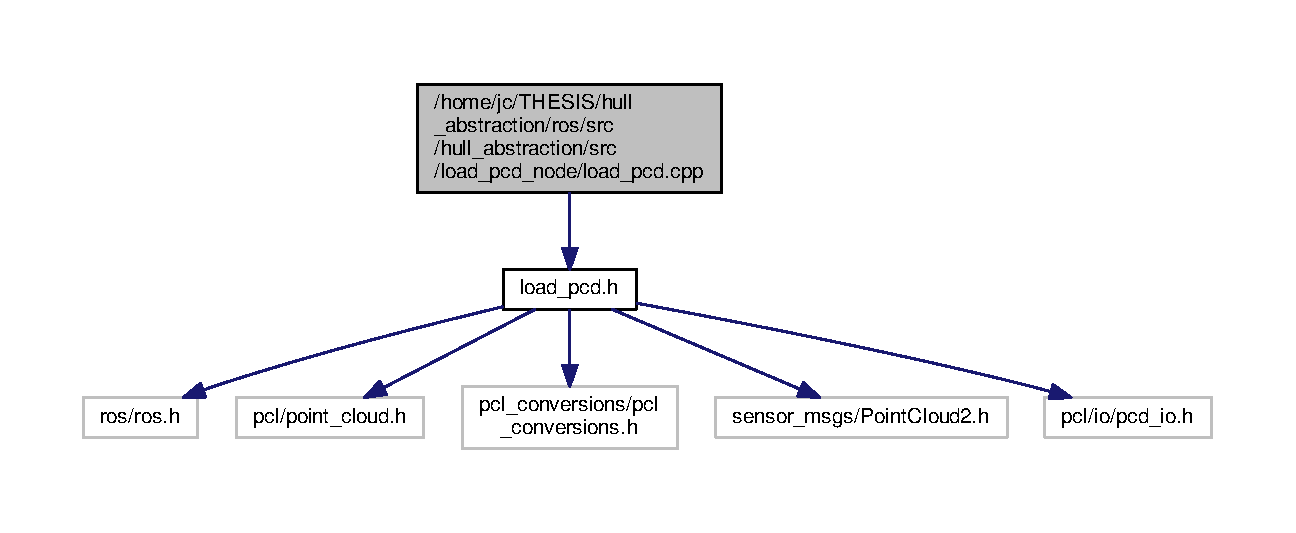
\includegraphics[width=350pt]{load__pcd_8cpp__incl}
\end{center}
\end{figure}

\hypertarget{load__pcd_8h}{}\section{/home/jc/hull\+\_\+abstraction/ros/src/hull\+\_\+abstraction/src/load\+\_\+pcd\+\_\+node/load\+\_\+pcd.h File Reference}
\label{load__pcd_8h}\index{/home/jc/hull\+\_\+abstraction/ros/src/hull\+\_\+abstraction/src/load\+\_\+pcd\+\_\+node/load\+\_\+pcd.\+h@{/home/jc/hull\+\_\+abstraction/ros/src/hull\+\_\+abstraction/src/load\+\_\+pcd\+\_\+node/load\+\_\+pcd.\+h}}


Framework of node for loading pcd files.  


{\ttfamily \#include $<$ros/ros.\+h$>$}\\*
{\ttfamily \#include $<$pcl/point\+\_\+cloud.\+h$>$}\\*
{\ttfamily \#include $<$pcl\+\_\+conversions/pcl\+\_\+conversions.\+h$>$}\\*
{\ttfamily \#include $<$sensor\+\_\+msgs/\+Point\+Cloud2.\+h$>$}\\*
{\ttfamily \#include $<$pcl/io/pcd\+\_\+io.\+h$>$}\\*
Include dependency graph for load\+\_\+pcd.\+h\+:\nopagebreak
\begin{figure}[H]
\begin{center}
\leavevmode
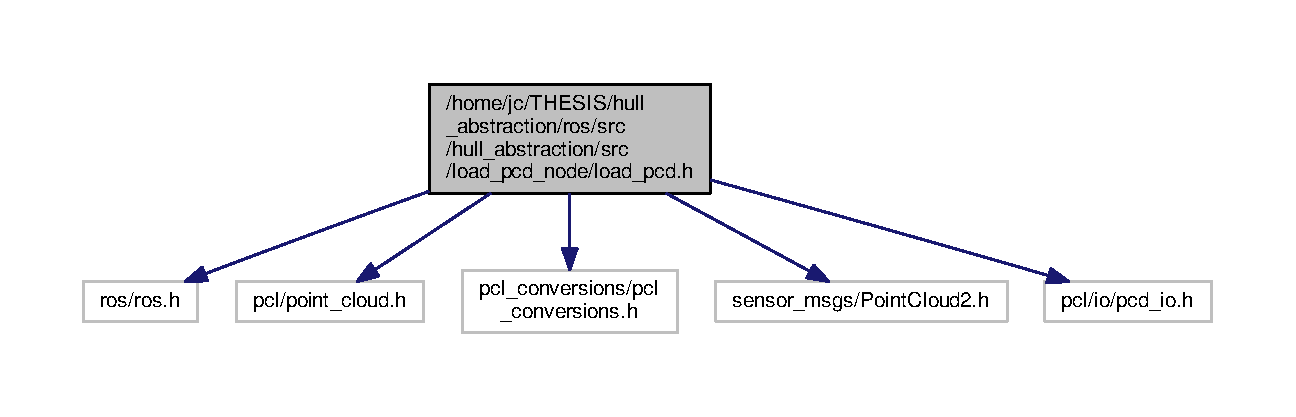
\includegraphics[width=350pt]{load__pcd_8h__incl}
\end{center}
\end{figure}
This graph shows which files directly or indirectly include this file\+:\nopagebreak
\begin{figure}[H]
\begin{center}
\leavevmode
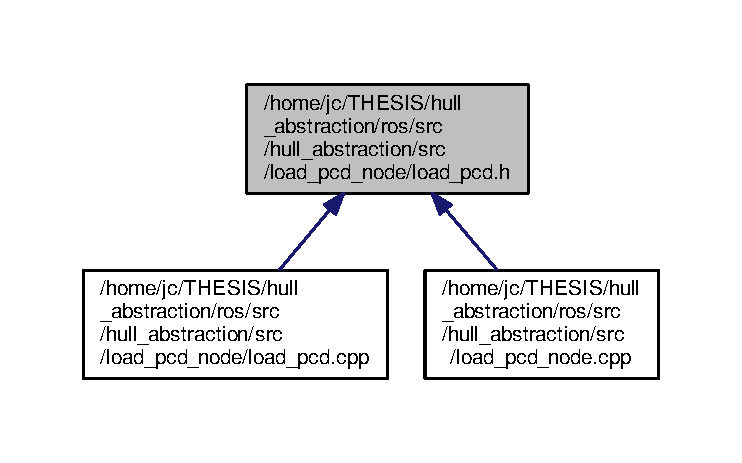
\includegraphics[width=350pt]{load__pcd_8h__dep__incl}
\end{center}
\end{figure}
\subsection*{Classes}
\begin{DoxyCompactItemize}
\item 
class \hyperlink{classload__pcd__node_1_1_load_p_c_d}{load\+\_\+pcd\+\_\+node\+::\+Load\+P\+CD}
\begin{DoxyCompactList}\small\item\em Class for loading pcd files. \end{DoxyCompactList}\end{DoxyCompactItemize}
\subsection*{Namespaces}
\begin{DoxyCompactItemize}
\item 
 \hyperlink{namespaceload__pcd__node}{load\+\_\+pcd\+\_\+node}
\end{DoxyCompactItemize}


\subsection{Detailed Description}
Framework of node for loading pcd files. 

\begin{DoxyAuthor}{Author}
Jiancong Zheng 
\end{DoxyAuthor}
\begin{DoxyDate}{Date}
2020-\/05-\/12
\end{DoxyDate}
This node load a local pcd file to get point cloud data and publish it as a R\+OS message. 
\hypertarget{marching__cubes__node_8cpp}{}\section{/home/jc/\+T\+H\+E\+S\+I\+S/hull\+\_\+abstraction/ros/src/hull\+\_\+abstraction/src/marching\+\_\+cubes\+\_\+node.cpp File Reference}
\label{marching__cubes__node_8cpp}\index{/home/jc/\+T\+H\+E\+S\+I\+S/hull\+\_\+abstraction/ros/src/hull\+\_\+abstraction/src/marching\+\_\+cubes\+\_\+node.\+cpp@{/home/jc/\+T\+H\+E\+S\+I\+S/hull\+\_\+abstraction/ros/src/hull\+\_\+abstraction/src/marching\+\_\+cubes\+\_\+node.\+cpp}}
{\ttfamily \#include \char`\"{}marching\+\_\+cubes\+\_\+node/marching\+\_\+cubes.\+h\char`\"{}}\\*
Include dependency graph for marching\+\_\+cubes\+\_\+node.\+cpp\+:
\nopagebreak
\begin{figure}[H]
\begin{center}
\leavevmode
\includegraphics[width=350pt]{marching__cubes__node_8cpp__incl}
\end{center}
\end{figure}
\subsection*{Functions}
\begin{DoxyCompactItemize}
\item 
int \hyperlink{marching__cubes__node_8cpp_a0ddf1224851353fc92bfbff6f499fa97}{main} (int argc, char $\ast$argv\mbox{[}$\,$\mbox{]})
\end{DoxyCompactItemize}


\subsection{Function Documentation}
\index{marching\+\_\+cubes\+\_\+node.\+cpp@{marching\+\_\+cubes\+\_\+node.\+cpp}!main@{main}}
\index{main@{main}!marching\+\_\+cubes\+\_\+node.\+cpp@{marching\+\_\+cubes\+\_\+node.\+cpp}}
\subsubsection[{\texorpdfstring{main(int argc, char $\ast$argv[])}{main(int argc, char *argv[])}}]{\setlength{\rightskip}{0pt plus 5cm}int main (
\begin{DoxyParamCaption}
\item[{int}]{argc, }
\item[{char $\ast$}]{argv\mbox{[}$\,$\mbox{]}}
\end{DoxyParamCaption}
)}\hypertarget{marching__cubes__node_8cpp_a0ddf1224851353fc92bfbff6f499fa97}{}\label{marching__cubes__node_8cpp_a0ddf1224851353fc92bfbff6f499fa97}

\hypertarget{marching__cubes_8cpp}{}\section{/home/jc/hull\+\_\+abstraction/ros/src/hull\+\_\+abstraction/src/marching\+\_\+cubes\+\_\+node/marching\+\_\+cubes.cpp File Reference}
\label{marching__cubes_8cpp}\index{/home/jc/hull\+\_\+abstraction/ros/src/hull\+\_\+abstraction/src/marching\+\_\+cubes\+\_\+node/marching\+\_\+cubes.\+cpp@{/home/jc/hull\+\_\+abstraction/ros/src/hull\+\_\+abstraction/src/marching\+\_\+cubes\+\_\+node/marching\+\_\+cubes.\+cpp}}
{\ttfamily \#include \char`\"{}marching\+\_\+cubes.\+h\char`\"{}}\\*
Include dependency graph for marching\+\_\+cubes.\+cpp\+:\nopagebreak
\begin{figure}[H]
\begin{center}
\leavevmode
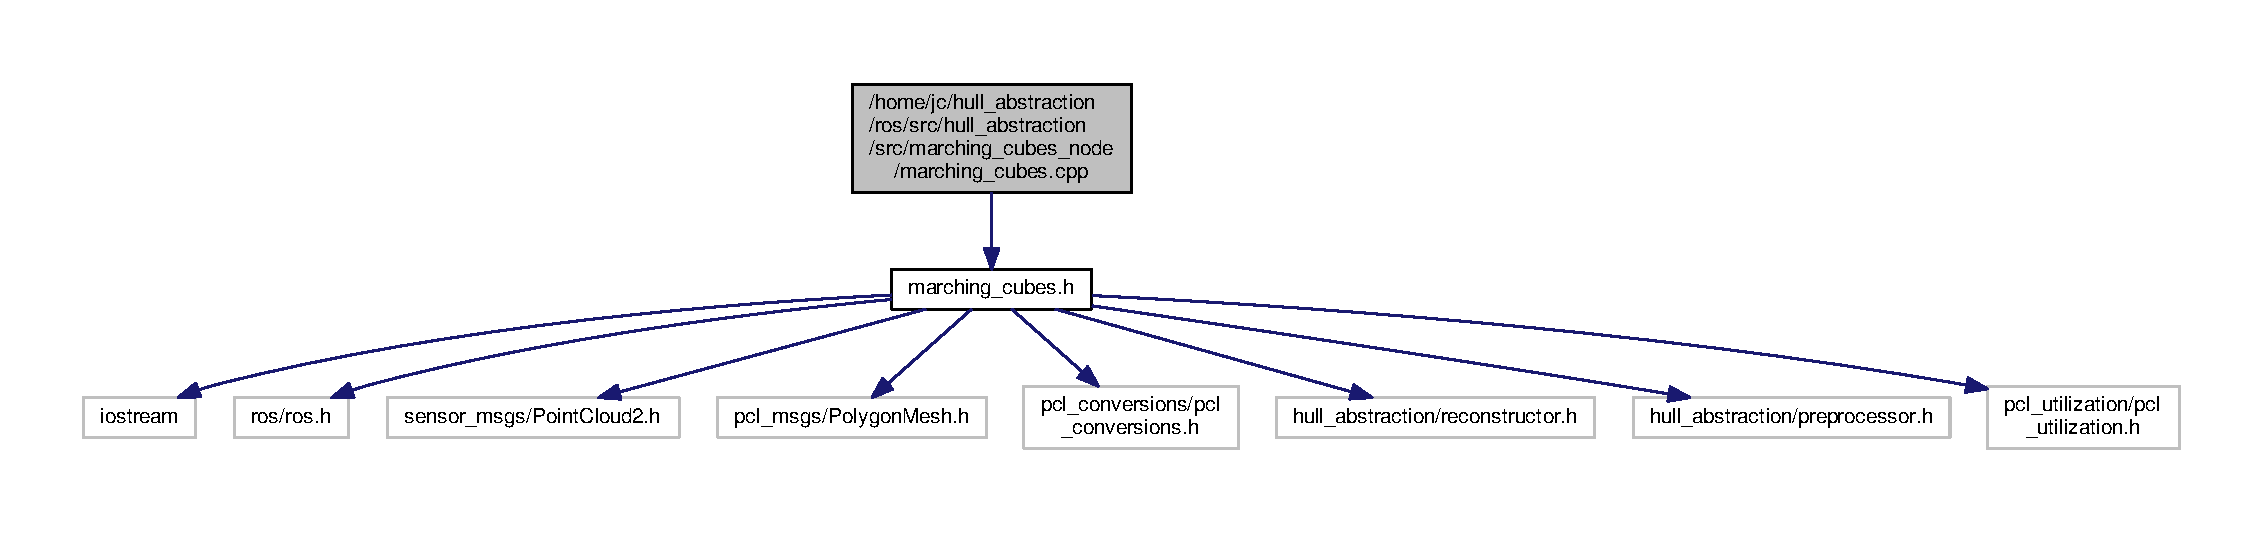
\includegraphics[width=350pt]{marching__cubes_8cpp__incl}
\end{center}
\end{figure}

\hypertarget{marching__cubes_8h}{}\section{/home/jc/hull\+\_\+abstraction/ros/src/hull\+\_\+abstraction/src/marching\+\_\+cubes\+\_\+node/marching\+\_\+cubes.h File Reference}
\label{marching__cubes_8h}\index{/home/jc/hull\+\_\+abstraction/ros/src/hull\+\_\+abstraction/src/marching\+\_\+cubes\+\_\+node/marching\+\_\+cubes.\+h@{/home/jc/hull\+\_\+abstraction/ros/src/hull\+\_\+abstraction/src/marching\+\_\+cubes\+\_\+node/marching\+\_\+cubes.\+h}}


Framework of marching cubes node.  


{\ttfamily \#include $<$iostream$>$}\\*
{\ttfamily \#include $<$ros/ros.\+h$>$}\\*
{\ttfamily \#include $<$sensor\+\_\+msgs/\+Point\+Cloud2.\+h$>$}\\*
{\ttfamily \#include $<$pcl\+\_\+msgs/\+Polygon\+Mesh.\+h$>$}\\*
{\ttfamily \#include $<$pcl\+\_\+conversions/pcl\+\_\+conversions.\+h$>$}\\*
{\ttfamily \#include \char`\"{}hull\+\_\+abstraction/reconstructor.\+h\char`\"{}}\\*
{\ttfamily \#include \char`\"{}hull\+\_\+abstraction/preprocessor.\+h\char`\"{}}\\*
{\ttfamily \#include \char`\"{}pcl\+\_\+utilization/pcl\+\_\+utilization.\+h\char`\"{}}\\*
Include dependency graph for marching\+\_\+cubes.\+h\+:\nopagebreak
\begin{figure}[H]
\begin{center}
\leavevmode
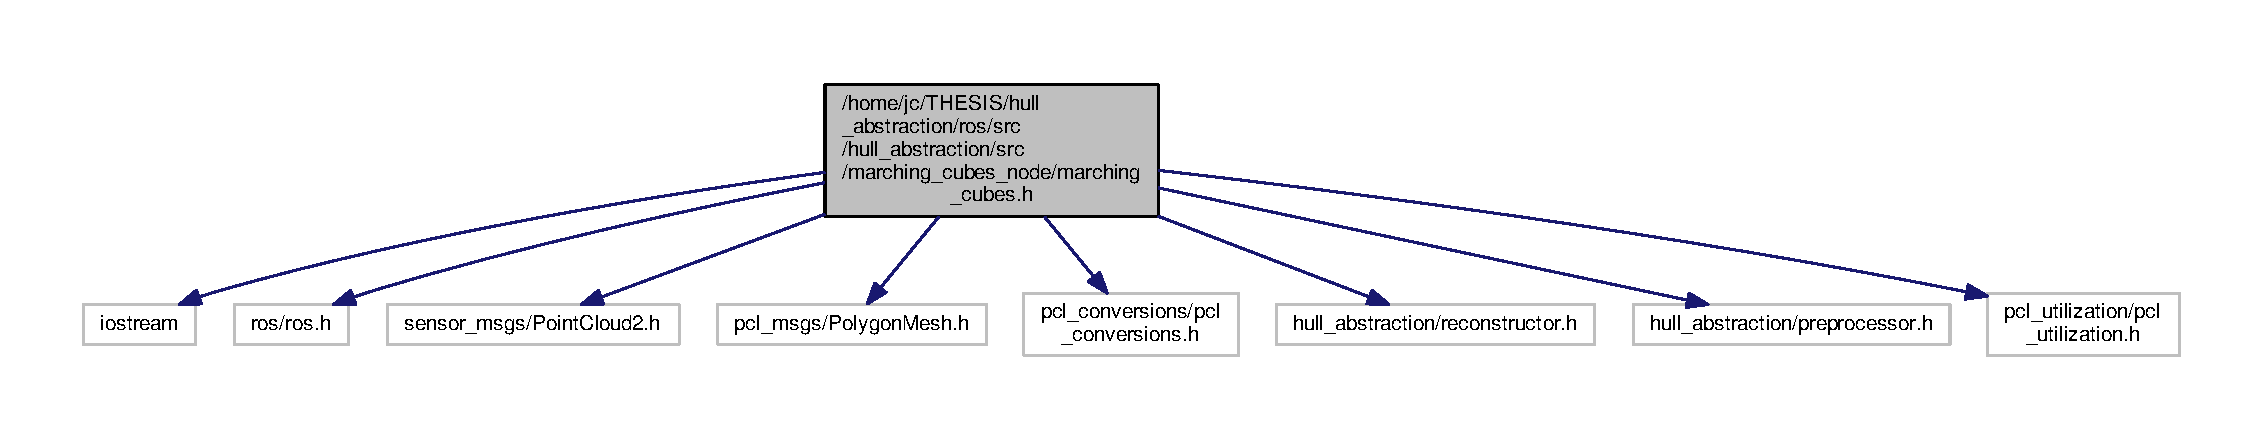
\includegraphics[width=350pt]{marching__cubes_8h__incl}
\end{center}
\end{figure}
This graph shows which files directly or indirectly include this file\+:\nopagebreak
\begin{figure}[H]
\begin{center}
\leavevmode
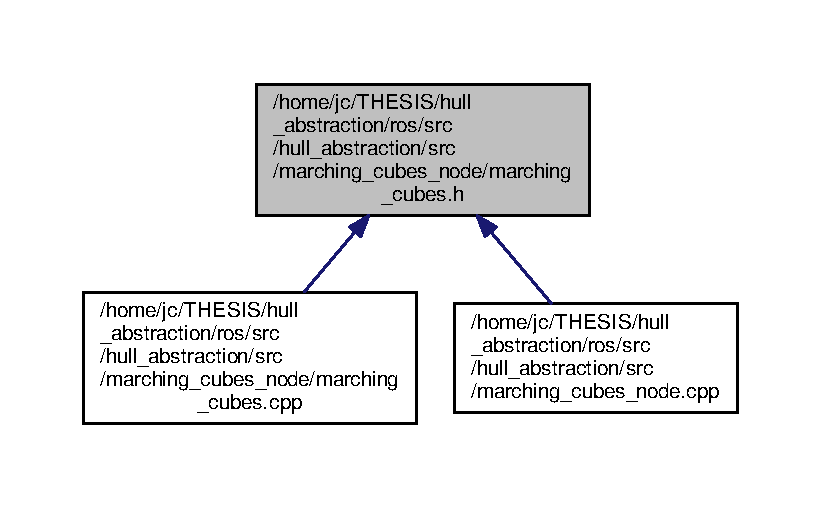
\includegraphics[width=350pt]{marching__cubes_8h__dep__incl}
\end{center}
\end{figure}
\subsection*{Classes}
\begin{DoxyCompactItemize}
\item 
class \hyperlink{classmarching__cubes_1_1_marching_cubes}{marching\+\_\+cubes\+::\+Marching\+Cubes}
\begin{DoxyCompactList}\small\item\em Class utilizing marching cubes method. \end{DoxyCompactList}\end{DoxyCompactItemize}
\subsection*{Namespaces}
\begin{DoxyCompactItemize}
\item 
 \hyperlink{namespacemarching__cubes}{marching\+\_\+cubes}
\end{DoxyCompactItemize}


\subsection{Detailed Description}
Framework of marching cubes node. 

\begin{DoxyRefDesc}{R\+O\+S Node}
\item[\hyperlink{ros_node__ros_node000005}{R\+O\+S Node}]marhcing\+\_\+cubes\+\_\+node\end{DoxyRefDesc}


\begin{DoxyAuthor}{Author}
Jiancong Zheng 
\end{DoxyAuthor}
\begin{DoxyDate}{Date}
2020-\/05-\/23
\end{DoxyDate}
This node subscribes a R\+OS topic to get an input point cloud and then utilize marching cubes algorithm to generate a mesh. The result of marching cubes is published as a pcl message. 
\hypertarget{moving__least__squares__node_8cpp}{}\section{/home/jc/\+T\+H\+E\+S\+I\+S/hull\+\_\+abstraction/ros/src/hull\+\_\+abstraction/src/moving\+\_\+least\+\_\+squares\+\_\+node.cpp File Reference}
\label{moving__least__squares__node_8cpp}\index{/home/jc/\+T\+H\+E\+S\+I\+S/hull\+\_\+abstraction/ros/src/hull\+\_\+abstraction/src/moving\+\_\+least\+\_\+squares\+\_\+node.\+cpp@{/home/jc/\+T\+H\+E\+S\+I\+S/hull\+\_\+abstraction/ros/src/hull\+\_\+abstraction/src/moving\+\_\+least\+\_\+squares\+\_\+node.\+cpp}}
{\ttfamily \#include \char`\"{}moving\+\_\+least\+\_\+squares\+\_\+node/moving\+\_\+least\+\_\+squares.\+h\char`\"{}}\\*
Include dependency graph for moving\+\_\+least\+\_\+squares\+\_\+node.\+cpp\+:
\nopagebreak
\begin{figure}[H]
\begin{center}
\leavevmode
\includegraphics[width=350pt]{moving__least__squares__node_8cpp__incl}
\end{center}
\end{figure}
\subsection*{Functions}
\begin{DoxyCompactItemize}
\item 
int \hyperlink{moving__least__squares__node_8cpp_a3c04138a5bfe5d72780bb7e82a18e627}{main} (int argc, char $\ast$$\ast$argv)
\end{DoxyCompactItemize}


\subsection{Function Documentation}
\index{moving\+\_\+least\+\_\+squares\+\_\+node.\+cpp@{moving\+\_\+least\+\_\+squares\+\_\+node.\+cpp}!main@{main}}
\index{main@{main}!moving\+\_\+least\+\_\+squares\+\_\+node.\+cpp@{moving\+\_\+least\+\_\+squares\+\_\+node.\+cpp}}
\subsubsection[{\texorpdfstring{main(int argc, char $\ast$$\ast$argv)}{main(int argc, char **argv)}}]{\setlength{\rightskip}{0pt plus 5cm}int main (
\begin{DoxyParamCaption}
\item[{int}]{argc, }
\item[{char $\ast$$\ast$}]{argv}
\end{DoxyParamCaption}
)}\hypertarget{moving__least__squares__node_8cpp_a3c04138a5bfe5d72780bb7e82a18e627}{}\label{moving__least__squares__node_8cpp_a3c04138a5bfe5d72780bb7e82a18e627}

\hypertarget{moving__least__squares_8cpp}{}\section{/home/jc/hull\+\_\+abstraction/ros/src/hull\+\_\+abstraction/src/moving\+\_\+least\+\_\+squares\+\_\+node/moving\+\_\+least\+\_\+squares.cpp File Reference}
\label{moving__least__squares_8cpp}\index{/home/jc/hull\+\_\+abstraction/ros/src/hull\+\_\+abstraction/src/moving\+\_\+least\+\_\+squares\+\_\+node/moving\+\_\+least\+\_\+squares.\+cpp@{/home/jc/hull\+\_\+abstraction/ros/src/hull\+\_\+abstraction/src/moving\+\_\+least\+\_\+squares\+\_\+node/moving\+\_\+least\+\_\+squares.\+cpp}}
{\ttfamily \#include \char`\"{}moving\+\_\+least\+\_\+squares.\+h\char`\"{}}\\*
Include dependency graph for moving\+\_\+least\+\_\+squares.\+cpp\+:\nopagebreak
\begin{figure}[H]
\begin{center}
\leavevmode
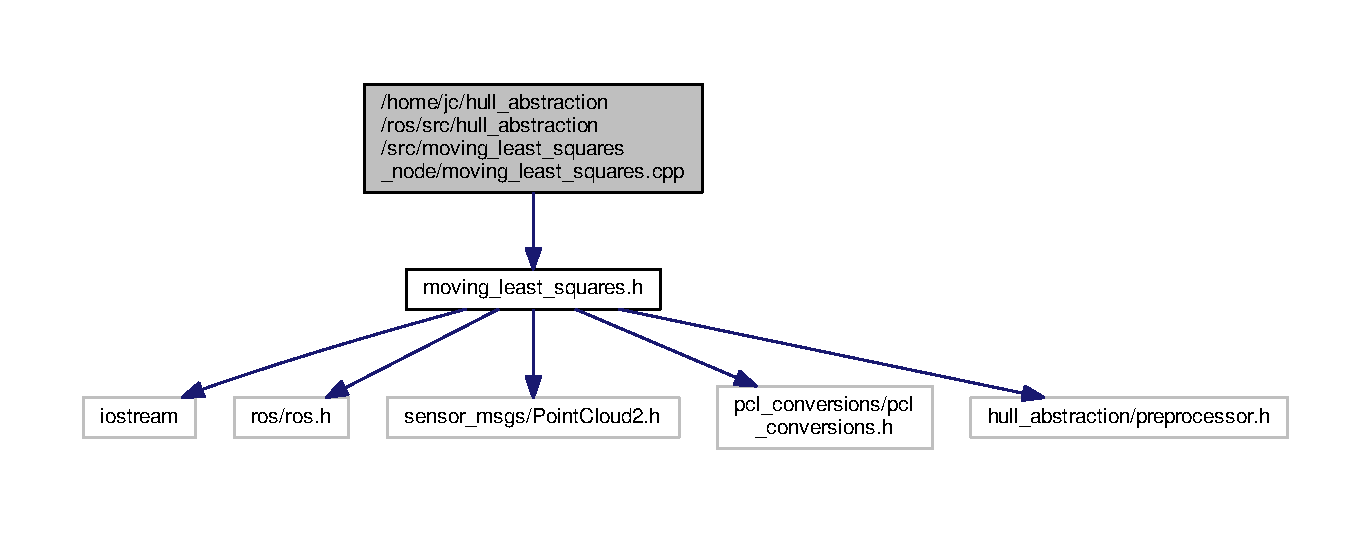
\includegraphics[width=350pt]{moving__least__squares_8cpp__incl}
\end{center}
\end{figure}

\hypertarget{moving__least__squares_8h}{}\section{/home/jc/hull\+\_\+abstraction/ros/src/hull\+\_\+abstraction/src/moving\+\_\+least\+\_\+squares\+\_\+node/moving\+\_\+least\+\_\+squares.h File Reference}
\label{moving__least__squares_8h}\index{/home/jc/hull\+\_\+abstraction/ros/src/hull\+\_\+abstraction/src/moving\+\_\+least\+\_\+squares\+\_\+node/moving\+\_\+least\+\_\+squares.\+h@{/home/jc/hull\+\_\+abstraction/ros/src/hull\+\_\+abstraction/src/moving\+\_\+least\+\_\+squares\+\_\+node/moving\+\_\+least\+\_\+squares.\+h}}


Framework of moving least squares node.  


{\ttfamily \#include $<$iostream$>$}\\*
{\ttfamily \#include $<$ros/ros.\+h$>$}\\*
{\ttfamily \#include $<$sensor\+\_\+msgs/\+Point\+Cloud2.\+h$>$}\\*
{\ttfamily \#include $<$pcl\+\_\+conversions/pcl\+\_\+conversions.\+h$>$}\\*
{\ttfamily \#include \char`\"{}hull\+\_\+abstraction/preprocessor.\+h\char`\"{}}\\*
Include dependency graph for moving\+\_\+least\+\_\+squares.\+h\+:\nopagebreak
\begin{figure}[H]
\begin{center}
\leavevmode
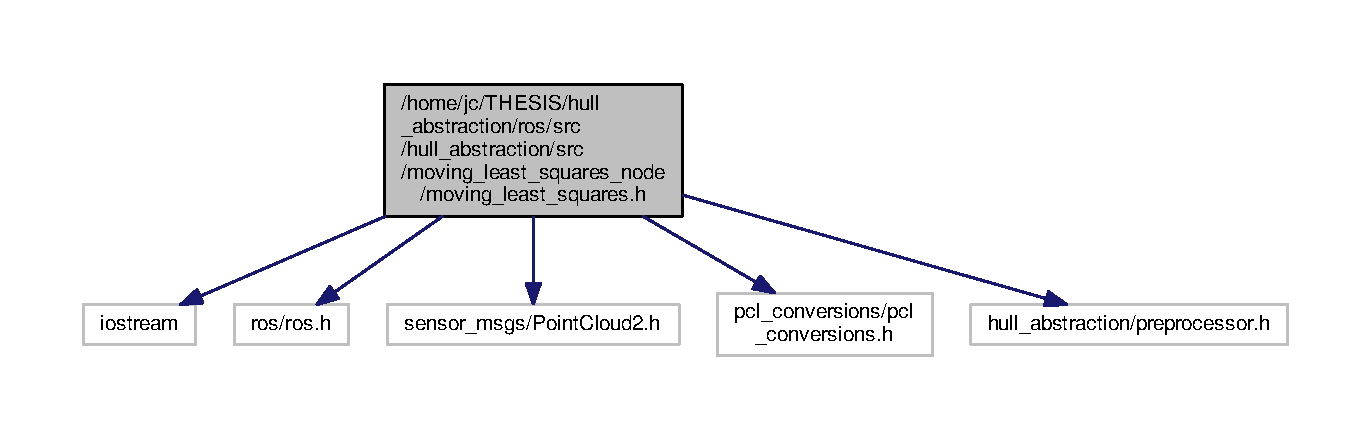
\includegraphics[width=350pt]{moving__least__squares_8h__incl}
\end{center}
\end{figure}
This graph shows which files directly or indirectly include this file\+:\nopagebreak
\begin{figure}[H]
\begin{center}
\leavevmode
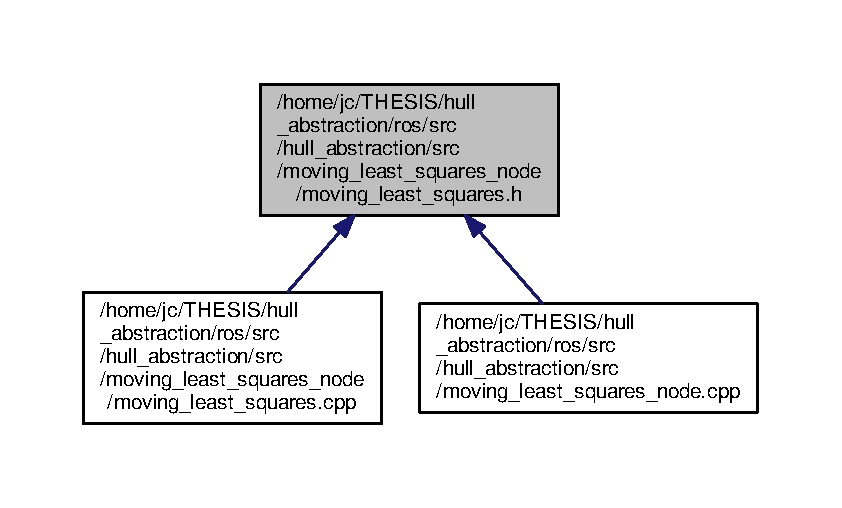
\includegraphics[width=350pt]{moving__least__squares_8h__dep__incl}
\end{center}
\end{figure}
\subsection*{Classes}
\begin{DoxyCompactItemize}
\item 
class \hyperlink{classmoving__least__squares__node_1_1_moving_least_squares}{moving\+\_\+least\+\_\+squares\+\_\+node\+::\+Moving\+Least\+Squares}
\begin{DoxyCompactList}\small\item\em Class utilizing moving least squares method. \end{DoxyCompactList}\end{DoxyCompactItemize}
\subsection*{Namespaces}
\begin{DoxyCompactItemize}
\item 
 \hyperlink{namespacemoving__least__squares__node}{moving\+\_\+least\+\_\+squares\+\_\+node}
\end{DoxyCompactItemize}


\subsection{Detailed Description}
Framework of moving least squares node. 

\begin{DoxyRefDesc}{R\+O\+S Node}
\item[\hyperlink{ros_node__ros_node000005}{R\+O\+S Node}]\hyperlink{namespacemoving__least__squares__node}{moving\+\_\+least\+\_\+squares\+\_\+node}\end{DoxyRefDesc}


\begin{DoxyAuthor}{Author}
Jiancong Zheng 
\end{DoxyAuthor}
\begin{DoxyDate}{Date}
2020-\/05-\/12
\end{DoxyDate}
This node subscribes a R\+OS topic to get an input point cloud and then utilize moving least squares method to make the point cloud smoother. M\+LS method can be seen as a preprocessing method. The result of moving least squares method is published as a point cloud message. 
\hypertarget{pcl__utilization_8cpp}{}\section{/home/jc/hull\+\_\+abstraction/ros/src/hull\+\_\+abstraction/src/pcl\+\_\+utilization/pcl\+\_\+utilization.cpp File Reference}
\label{pcl__utilization_8cpp}\index{/home/jc/hull\+\_\+abstraction/ros/src/hull\+\_\+abstraction/src/pcl\+\_\+utilization/pcl\+\_\+utilization.\+cpp@{/home/jc/hull\+\_\+abstraction/ros/src/hull\+\_\+abstraction/src/pcl\+\_\+utilization/pcl\+\_\+utilization.\+cpp}}
{\ttfamily \#include \char`\"{}pcl\+\_\+utilization/pcl\+\_\+utilization.\+h\char`\"{}}\\*
Include dependency graph for pcl\+\_\+utilization.\+cpp\+:\nopagebreak
\begin{figure}[H]
\begin{center}
\leavevmode
\includegraphics[width=350pt]{pcl__utilization_8cpp__incl}
\end{center}
\end{figure}

\hypertarget{poisson__reconstruction__node_8cpp}{}\section{/home/jc/hull\+\_\+abstraction/ros/src/hull\+\_\+abstraction/src/poisson\+\_\+reconstruction\+\_\+node.cpp File Reference}
\label{poisson__reconstruction__node_8cpp}\index{/home/jc/hull\+\_\+abstraction/ros/src/hull\+\_\+abstraction/src/poisson\+\_\+reconstruction\+\_\+node.\+cpp@{/home/jc/hull\+\_\+abstraction/ros/src/hull\+\_\+abstraction/src/poisson\+\_\+reconstruction\+\_\+node.\+cpp}}
{\ttfamily \#include \char`\"{}poisson\+\_\+reconstruction\+\_\+node/poisson\+\_\+reconstruction.\+h\char`\"{}}\\*
Include dependency graph for poisson\+\_\+reconstruction\+\_\+node.\+cpp\+:\nopagebreak
\begin{figure}[H]
\begin{center}
\leavevmode
\includegraphics[width=350pt]{poisson__reconstruction__node_8cpp__incl}
\end{center}
\end{figure}
\subsection*{Functions}
\begin{DoxyCompactItemize}
\item 
int \hyperlink{poisson__reconstruction__node_8cpp_a3c04138a5bfe5d72780bb7e82a18e627}{main} (int argc, char $\ast$$\ast$argv)
\end{DoxyCompactItemize}


\subsection{Function Documentation}
\index{poisson\+\_\+reconstruction\+\_\+node.\+cpp@{poisson\+\_\+reconstruction\+\_\+node.\+cpp}!main@{main}}
\index{main@{main}!poisson\+\_\+reconstruction\+\_\+node.\+cpp@{poisson\+\_\+reconstruction\+\_\+node.\+cpp}}
\subsubsection[{\texorpdfstring{main(int argc, char $\ast$$\ast$argv)}{main(int argc, char **argv)}}]{\setlength{\rightskip}{0pt plus 5cm}int main (
\begin{DoxyParamCaption}
\item[{int}]{argc, }
\item[{char $\ast$$\ast$}]{argv}
\end{DoxyParamCaption}
)}\hypertarget{poisson__reconstruction__node_8cpp_a3c04138a5bfe5d72780bb7e82a18e627}{}\label{poisson__reconstruction__node_8cpp_a3c04138a5bfe5d72780bb7e82a18e627}

\hypertarget{poisson__reconstruction_8cpp}{}\section{/home/jc/\+T\+H\+E\+S\+I\+S/hull\+\_\+abstraction/ros/src/hull\+\_\+abstraction/src/poisson\+\_\+reconstruction\+\_\+node/poisson\+\_\+reconstruction.cpp File Reference}
\label{poisson__reconstruction_8cpp}\index{/home/jc/\+T\+H\+E\+S\+I\+S/hull\+\_\+abstraction/ros/src/hull\+\_\+abstraction/src/poisson\+\_\+reconstruction\+\_\+node/poisson\+\_\+reconstruction.\+cpp@{/home/jc/\+T\+H\+E\+S\+I\+S/hull\+\_\+abstraction/ros/src/hull\+\_\+abstraction/src/poisson\+\_\+reconstruction\+\_\+node/poisson\+\_\+reconstruction.\+cpp}}
{\ttfamily \#include \char`\"{}poisson\+\_\+reconstruction.\+h\char`\"{}}\\*
Include dependency graph for poisson\+\_\+reconstruction.\+cpp\+:
\nopagebreak
\begin{figure}[H]
\begin{center}
\leavevmode
\includegraphics[width=350pt]{poisson__reconstruction_8cpp__incl}
\end{center}
\end{figure}

\hypertarget{poisson__reconstruction_8h}{}\section{/home/jc/hull\+\_\+abstraction/ros/src/hull\+\_\+abstraction/src/poisson\+\_\+reconstruction\+\_\+node/poisson\+\_\+reconstruction.h File Reference}
\label{poisson__reconstruction_8h}\index{/home/jc/hull\+\_\+abstraction/ros/src/hull\+\_\+abstraction/src/poisson\+\_\+reconstruction\+\_\+node/poisson\+\_\+reconstruction.\+h@{/home/jc/hull\+\_\+abstraction/ros/src/hull\+\_\+abstraction/src/poisson\+\_\+reconstruction\+\_\+node/poisson\+\_\+reconstruction.\+h}}


Framework of Poisson reconstruction node.  


{\ttfamily \#include $<$iostream$>$}\\*
{\ttfamily \#include $<$ros/ros.\+h$>$}\\*
{\ttfamily \#include $<$sensor\+\_\+msgs/\+Point\+Cloud2.\+h$>$}\\*
{\ttfamily \#include $<$pcl\+\_\+msgs/\+Polygon\+Mesh.\+h$>$}\\*
{\ttfamily \#include $<$pcl\+\_\+conversions/pcl\+\_\+conversions.\+h$>$}\\*
{\ttfamily \#include \char`\"{}hull\+\_\+abstraction/reconstructor.\+h\char`\"{}}\\*
{\ttfamily \#include \char`\"{}hull\+\_\+abstraction/preprocessor.\+h\char`\"{}}\\*
Include dependency graph for poisson\+\_\+reconstruction.\+h\+:\nopagebreak
\begin{figure}[H]
\begin{center}
\leavevmode
\includegraphics[width=350pt]{poisson__reconstruction_8h__incl}
\end{center}
\end{figure}
This graph shows which files directly or indirectly include this file\+:\nopagebreak
\begin{figure}[H]
\begin{center}
\leavevmode
\includegraphics[width=350pt]{poisson__reconstruction_8h__dep__incl}
\end{center}
\end{figure}
\subsection*{Classes}
\begin{DoxyCompactItemize}
\item 
class \hyperlink{classpoisson__reconstruction_1_1_poisson_reconstruction}{poisson\+\_\+reconstruction\+::\+Poisson\+Reconstruction}
\begin{DoxyCompactList}\small\item\em Class utilizing Poisson reconstruction method. \end{DoxyCompactList}\end{DoxyCompactItemize}
\subsection*{Namespaces}
\begin{DoxyCompactItemize}
\item 
 \hyperlink{namespacepoisson__reconstruction}{poisson\+\_\+reconstruction}
\end{DoxyCompactItemize}


\subsection{Detailed Description}
Framework of Poisson reconstruction node. 

\begin{DoxyRefDesc}{R\+O\+S Node}
\item[\hyperlink{ros_node__ros_node000006}{R\+O\+S Node}]poisson\+\_\+reconstruction\+\_\+node\end{DoxyRefDesc}


\begin{DoxyAuthor}{Author}
Jiancong Zheng 
\end{DoxyAuthor}
\begin{DoxyDate}{Date}
2020-\/05-\/12
\end{DoxyDate}
This node subscribes a R\+OS topic to get an input point cloud and then utilize Poisson reconstruction to generate a mesh. The result of Poisson reconstruction is published as a point cloud message. 
%--- End generated contents ---

% Index
\backmatter
\newpage
\phantomsection
\clearemptydoublepage
\addcontentsline{toc}{chapter}{Index}
\printindex

\end{document}
